% Gelfand seminar notes, 1967-68 and 1968-69: source pages P000208-P000284.
% Russian diplomatic transcription (AI-made, checked against the scans), cut page by page from the cumulative working reader A4-reader-chapters01-27-first1252-separated-diplomatic-r4.
% \SourcePage{GELFAND-Pnnnnnn}{label} starts a scanned page; the second argument is the number written
% on the page, if any. Editorial notes give the page, a label and the transcriber's remark; \Unclear
% marks a doubtful reading.
\SourcePage{GELFAND-P000208}{1}
\begin{flushright}$1$\end{flushright}



\underline{\underline{1967 год.}}\qquad\underline{Сем. Гельфанда.}



$18/\overline{\underline{\mathrm{IX}}}$.\quad\underline{\underline{Кириллов.}}



\underline{Ф-ла}\quad\underline{(без док-ва и противор. примеров)}\quad\underline{характеров}
\par\underline{неприв. предст. групп Ли.}



\begin{equation*}\chi(x)=p(x)^{-1/2}\int_{\Omega}e^{i\langle F,x\rangle}\beta\qquad(\beta=\beta(F))\end{equation*}



$x\in\mathfrak g$,\quad$F\in\mathfrak g^*$,\quad$\Omega$ --- орбита в $\mathfrak g^*$ относит. $G$,
\par$\beta$ --- диффер. форма,\quad$p(x)$ --- плотность меры Хаара.



\begin{GelfandAdjacentEvidence}{GELFAND-P000208}{1}
(Орбиты не все, а нек-рые, удовл. усл. целочисл., точно [формулируемый / формулируемым?]\}.
\Unclear{GELFAND-P000208}{integrality-ending}{Окончание последнего слова слито: «формулируемый» / «формулируемым». Правый замыкающий знак имеет изломы, как у фигурной скобки; в строке кандидат $\}$.}
\end{GelfandAdjacentEvidence}

($G$ --- группа,\quad$T$ --- унит. предст.,\quad$\chi(g)=\operatorname{tr}T(g)$\quad(в конечном.)



\begin{GelfandAdjacentEvidence}{GELFAND-P000208}{2}
В общем случае $\chi$ --- обобщ. функция
\begin{equation*}\langle\chi,\varphi\rangle=\int_G\varphi(g)T(g)\,dg\quad\text{--- уже есть след.}\end{equation*}
(Такое опред. хар.).)





\SourceFigure{GELFAND-P000208}{orbit-action}{\par\smallskip\centering{\color{black}$G$ действует в
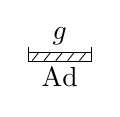
\begin{tikzpicture}[x=1mm,y=1mm,baseline=(alg.base)]
\node[inner sep=0pt] (alg) at (0,0) {$\mathfrak g$};
\draw[line width=.4pt] (-4,-1.3)--(-4,-3.2)--(4,-3.2)--(4,-1.3);
\draw[line width=.4pt] (-4,-2)--(4,-2);
\draw[line width=.3pt] (-3.5,-3.1)--(-2.7,-2.1) (-2,-3.1)--(-1.2,-2.1) (-.5,-3.1)--(.3,-2.1) (1,-3.1)--(1.8,-2.1) (2.5,-3.1)--(3.3,-2.1);
\node[anchor=north,inner sep=1pt] at (0,-3.5) {$\mathrm{Ad}$};
\end{tikzpicture}
и в $\mathfrak g^*$, там система орбит.
}}
\end{GelfandAdjacentEvidence}

Всё это в малой окр. $e$ --- где есть \underline{\underline{$\exp$}}.



$\beta$ строится по структ. конст. алгебры.



\begin{GelfandAdjacentEvidence}{GELFAND-P000208}{3}
[Зачёркнуто: неразборчиво.]
\Incomplete{GELFAND-P000208}{cancelled-word}{Одно слово под густыми повторяющимися петлями. Неустановленные кандидаты: «Предложения» / «Продолжение». Буквы под штрихами неразборчивы.}
\end{GelfandAdjacentEvidence}

\begin{center}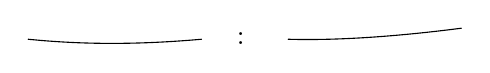
\begin{tikzpicture}[x=1mm,y=1mm]
\draw[line cap=round] (0,0).. controls (7,-.7) and (14,-.7)..(22,0);
\node[inner sep=0pt] at (27,.1) {:};
\draw[line cap=round] (33,0).. controls (40,-.2) and (48,.5)..(55,1.4);
\end{tikzpicture}\end{center}



\underline{Запланированы.}



1.\quad\uwave{Учебные доклады по логике.}\quad(включая решение континуум-гипотезы)



2.\quad Лидский «Асимптотика собств. знач. самосопр. опер.»



3.\quad Раб. Кириллова; Каждана; Граева.



\begin{center}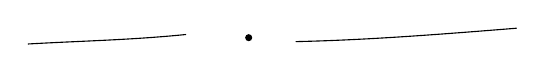
\begin{tikzpicture}[x=1mm,y=1mm]
\draw[line cap=round] (0,0).. controls (7,.4) and (13,.5)..(20,1.2);
\fill (28,.8) circle (.45mm);
\draw[line cap=round] (34,.3).. controls (43,.5) and (52,1.2)..(62,2);
\end{tikzpicture}\end{center}



\underline{Пример.}\quad$G=SO(3)$,\quad$\mathfrak g=\mathbb R^3$,\quad$\mathfrak g^*=\mathbb R^3$,
\par действие --- вращения.
\par Орбита --- $S^2$.



\begin{GelfandAdjacentEvidence}{GELFAND-P000208}{4}
\begin{equation*}p(x)=\frac{\sin\tau}{\tau},\qquad\text{где }\tau=\lVert x\rVert.\end{equation*}
\Unclear{GELFAND-P000208}{radial-density}{Повторяющийся знак радиальной переменной имеет верхнюю черту и загнутую ножку: $\tau$ / $r$. В строке кандидат $\tau$; буквенное чтение не установлено. Квадрат дроби не различим.}
\end{GelfandAdjacentEvidence}

Факт из анализа\quad(о преобр. Фурье $\delta$ на $S_\lambda$)



\begin{GelfandAdjacentEvidence}{GELFAND-P000208}{5}
\begin{equation*}\left(\delta_{S_\lambda}\right)^{\vee}\equiv\frac{\sin\lambda\tau}{\tau}\end{equation*}
\Unclear{GELFAND-P000208}{fourier-sphere}{Над закрывающей скобкой короткий двухштриховой знак: $\sim$ / $\vee$. Густой знак между скобкой и дробью: $\equiv$ / $=$. В строке кандидаты $\vee$, $\equiv$; оба чтения не установлены. Радиальная переменная та же, что в предыдущей дроби: $\tau$ / $r$.}
\end{GelfandAdjacentEvidence}



\SourcePage{GELFAND-P000209}{unlabelled}
$\beta$ --- обычн. поверхн. сферы.



\begin{GelfandAdjacentEvidence}{GELFAND-P000209}{1}
\underline{Ответ.}
\begin{equation*}\chi(x)=\frac{\sin\lambda\tau}{\sin\tau}.\end{equation*}
\Unclear{GELFAND-P000209}{radial-character}{Радиальная графема та же, что на предыдущей странице: $\tau$ / $r$. В дроби кандидат $\tau$; чтение буквы не установлено.}
\end{GelfandAdjacentEvidence}

Всё это при $\lambda=2n+1$ (счётн. число предст.)



$\beta(x)$ --- $\int$ по циклам орбиты от нек-рых форм целочисленных.



\uwave{Работа Фукса и Гельфанда.}



\underline{\underline{Фукс.}} Исслед. главных расслоений



\begin{GelfandAdjacentEvidence}{GELFAND-P000209}{2}
[Зачёркнуто: неразборчиво.]
\Incomplete{GELFAND-P000209}{cancelled-before-fiber}{Короткая густо зачёркнутая запись между «расслоений» и «со слоем». Буквы не установлены.}
\end{GelfandAdjacentEvidence}

со слоем $G$ (топ. группа)



Типы инвар. --- как топ. пр-ва и классиф. пр-ва.



\begin{GelfandAdjacentEvidence}{GELFAND-P000209}{3}
$\mathfrak g$ --- группа
\Unclear{GELFAND-P000209}{group-letter}{Петлеобразный групповой знак: строчное фрактуроподобное $\mathfrak g$ / рукописное прописное $G$. Кандидат $\mathfrak g$ повторён в индексах, подписях стрелок и под шляпкой; прямое $G$ выше имеет другое начертание. Регистр не установлен.}
\end{GelfandAdjacentEvidence}
\begin{GelfandAdjacentEvidence}{GELFAND-P000209}{4}




\SourceFigure{GELFAND-P000209}{universal-bundle}{\par\smallskip\centering{\color{black}\(\displaystyle 
\begin{tikzcd}[ampersand replacement=\&]E_{\mathfrak g}\arrow[d,"\mathfrak g"]\\B_{\mathfrak g}\end{tikzcd}
\qquad\text{--- универс. расслоение}
\)}}
\end{GelfandAdjacentEvidence}
\begin{GelfandAdjacentEvidence}{GELFAND-P000209}{5}

($E_{\mathfrak g}$ [Зачёркнуто: неразборчиво.]
\Incomplete{GELFAND-P000209}{cancelled-before-aspherical}{Одно слово под повторными густыми штрихами перед «асферично». Буквы не установлены.}
\end{GelfandAdjacentEvidence}

асферично, т.е. $\pi_k(E_{\mathfrak g})=0$, $k>0$).



Хар. класс опред. заданием $\alpha\in H^q(B_{\mathfrak g};A)$



\begin{GelfandAdjacentEvidence}{GELFAND-P000209}{6}
(Отобр. главных рассл. [перестан. / перестав.] с действием группы).
\Unclear{GELFAND-P000209}{equivariance-word}{Перед точкой в сокращении «перестан.» / «перестав.» предпоследние штрихи слиты. Оба чтения не установлены.}
\end{GelfandAdjacentEvidence}

Аналогично вместо $H^q$ --- любой контравар. функтор $h$ в категорию множеств.



Все хар. классы --- $h(B_{\mathfrak g})$



(это если $h$ --- гомотопич. функтор)



$\hat{\mathfrak g}$ --- макс. комп. подгруппа



(все они $\underset{\text{и экв. }\mathfrak g.}{\text{гомот. экв.}}$ и их классиф. пр-ва гом. эквивал.)



\begin{GelfandAdjacentEvidence}{GELFAND-P000209}{7}
Г. \underline{Задача:} найти настоящее классиф. пр-во некомп. групп,
не отожд. её с макс. комп. подгр.






\SourceFigure{GELFAND-P000209}{Hausdorff-bundle}{\par\smallskip\centering{\color{black}\(\displaystyle 
\begin{tikzcd}[ampersand replacement=\&]E\arrow[d,"\mathfrak g"]\\X\end{tikzcd}
\qquad\begin{aligned}
&\text{база \uwave{только хаусдорфова}}\\
&\text{условие, замен. лок. тривиальность,}\\
&\text{к-рое в вполне регул. случае совп.}\\
&\text{с обыч}\underline{\text{ной}}\text{ лок. трив.}
\end{aligned}
\)}}
\end{GelfandAdjacentEvidence}



\SourcePage{GELFAND-P000210}{2}
\begin{flushright}$2$\end{flushright}



Требуется выполнение след. свойства:



\begin{GelfandAdjacentEvidence}{GELFAND-P000210}{1}
\uwave{рассмотрим конус над $\mathfrak g$}
\Unclear{GELFAND-P000210}{cone-heading}{Петлеобразный знак группы тот же, что на предыдущей странице: фрактуроподобное строчное $\mathfrak g$ / рукописное прописное $G$. В строках и схемах кандидат $\mathfrak g$; регистр не установлен. Под заголовком волнистая черта.}
\end{GelfandAdjacentEvidence}
\begin{GelfandAdjacentEvidence}{GELFAND-P000210}{2}





\Unclear{GELFAND-P000210}{cone-sketch}{Внешний контур конуса, округлое основание и внутренние дугообразные ходы. замкнутость ходов и возможные направления стрелок не установлены.\par\smallskip\centering{\color{black}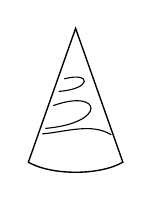
\begin{tikzpicture}[x=1mm,y=1mm,line cap=round]
\draw[line width=.5pt] (-6,0)--(0,17)--(6,0);
\draw[line width=.5pt] (-6,0)..controls(-3,-1.7)and(3,-1.7)..(6,0);
\draw[line width=.4pt] (-1.4,10.6)..controls(2,11.5)and(2.1,9.3)..(-2.1,9.0);
\draw[line width=.4pt] (-2.8,7.2)..controls(3.3,9.4)and(4.1,5.0)..(-3.8,4.3);
\draw[line width=.4pt] (-4.2,3.6)..controls(-1,3.9)and(2,5.0)..(4.5,3.5);
\end{tikzpicture}}}
\end{GelfandAdjacentEvidence}

на нём действ. $\mathfrak g$ с одной неподв. точкой.



$\forall x\in X$, $\exists$ отобр. $E\longrightarrow C\mathfrak g$, перестан.



\begin{GelfandAdjacentEvidence}{GELFAND-P000210}{3}
с действием группы, слой над [Зачёркнуто: неразборчивый знак.]
\Incomplete{GELFAND-P000210}{cancelled-point}{Перед $x$ густо зачёркнут знак с нижней петлёй. Неустановленные кандидаты: $y$ / $g$.}
\end{GelfandAdjacentEvidence}

$x$ изоморфно отображается на основание конуса



(Отсюда вытекает лок. тривиальность).



(Для вполне регул. базы (сущ. ф-я $1$ в точке, $0$ вне зад. окр.)



лок. тривиальность $\Longrightarrow$ это свойство.)



(но в этом случае теория тривиализуется и все вычисл. инварианты тривиальны)



\begin{center}\begin{tikzpicture}[x=1mm,y=1mm]
\draw[line cap=round] (0,0)..controls(4,-.3)and(8,-.1)..(12,.1);
\fill (18,.3) circle(.22mm);
\draw[line cap=round] (24,.6)..controls(28,.9)and(33,.8)..(37,.9);
\end{tikzpicture}\end{center}



\uwave{Замечание Д. Каждана}: тогда высота конуса определяет непр. ф-ю на $X$.



Так что это опред. неверно.



\begin{center}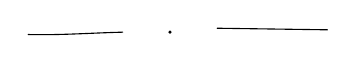
\begin{tikzpicture}[x=1mm,y=1mm]
\draw[line cap=round] (0,0)..controls(4,-.1)and(8,.2)..(12,.3);
\fill (18,.3) circle(.22mm);
\draw[line cap=round] (24,.8)--(38,.6);
\end{tikzpicture}\end{center}



\begin{GelfandAdjacentEvidence}{GELFAND-P000210}{4}
$\mathfrak g$ --- группа Ли,\quad$\mathfrak g\subset gL(n,\mathbb R)$ --- замкн. подгруппа.
\Unclear{GELFAND-P000210}{linear-group-case}{Первая буква перед $L$ имеет нижнюю петлю: $gL(n,\mathbb R)$ / $GL(n,\mathbb R)$. В строке кандидат $gL$; регистр не установлен. Знак самой группы тот же, что в заголовке о конусе.}
\end{GelfandAdjacentEvidence}

(т.е. $\mathfrak g$ действ. на $\mathbb R^n$).



Сущ. конструкция, к-рая по главному рассл. делает векторное (индуц.)



$E^*=E\times\mathbb R^n/\mathfrak g$.



\begin{GelfandAdjacentEvidence}{GELFAND-P000210}{5}
$(x,y)=(gx,gy)$
\Unclear{GELFAND-P000210}{quotient-relation}{Между парами два коротких густых штриха, слитых с левой скобкой правой пары: $=$ / $\sim$. В строке кандидат $=$; знак не установлен.}
\end{GelfandAdjacentEvidence}
\begin{GelfandAdjacentEvidence}{GELFAND-P000210}{6}




\SourceFigure{GELFAND-P000210}{vector-bundle-diagram}{\par\smallskip\centering{\color{black}\(\displaystyle \begin{tikzcd}[ampersand replacement=\&]E^*\arrow[r]\arrow[d,"{\mathbb R^n}"]\&\mathbb R^n\\X\&\end{tikzcd}\)}}
\end{GelfandAdjacentEvidence}

Должно сущ. отобр. $E^*\longrightarrow\mathbb R^n$,



\begin{GelfandAdjacentEvidence}{GELFAND-P000210}{7}
[Зачёркнуто: неразборчиво.]
\Incomplete{GELFAND-P000210}{cancelled-linear}{Короткое слово перед «линейное» зачёркнуто двумя чертами. Буквы не установлены.}
\end{GelfandAdjacentEvidence}

линейное по слоям и



такое что в нек-рой точке $x_0$\quad$\underset{\text{(данной)}}{\phantom{x_0}}$



оно --- изоморфизм.



(Никакого согласов. с действ. группы).




\begin{tikzpicture}[x=1mm,y=1mm]
\draw[line cap=round] (0,25)..controls(-5,17)and(-5,7)..(0,0);
\fill (0,0) circle(.3mm);
\end{tikzpicture}



это опред. лок. тривиальности (для хаусд.) и это и есть требование.



Замечание Каждана повт. нельзя.





\SourcePage{GELFAND-P000211}{unlabelled}
По $E^*$ восстанавливается $E$.



Постр. классиф. пр-во нельзя, но аналог есть.



\underline{Пример}:



\begin{GelfandAdjacentEvidence}{GELFAND-P000211}{1}
[Неустановленный утолщённый знак.]
\Unclear{GELFAND-P000211}{before-group}{Перед обозначением группы отдельный утолщённый знак с нижней петлёй и поперечным штрихом: «в» / зачёркнутый прежний знак. Ни один кандидат не установлен.}
\end{GelfandAdjacentEvidence}
\begin{GelfandAdjacentEvidence}{GELFAND-P000211}{2}

$\mathfrak g=\mathbb R\subset gL(1,\mathbb R)$ --- матрицы с $\det>0$.
\Unclear{GELFAND-P000211}{linear-group-case}{Первая буква перед $L$ с нижней петлёй: $gL$ / $GL$. В строке кандидат $gL$; регистр не установлен. Петлеобразный знак самой группы тот же, что на предыдущих страницах: $\mathfrak g$ / $G$, кандидат $\mathfrak g$.}
\end{GelfandAdjacentEvidence}

\uwave{Нетривиальное} $\underset{\text{(главное)}}{\mathbb R\text{-расслоение}}$ (оно же «универсально»).



Прямое произв. счётн. числа прямых в тих. топологии.



\begin{equation*}(x_1,x_2,\ldots)\quad\text{--- последовательности}\end{equation*}



\begin{equation*}\alpha(x_1,\ldots)=(x_1e^\alpha,\ldots)\end{equation*}



Факторпр-во $S$ нельзя вложить в $E$ (!) ---
--- нет сечений.



\underline{Факт:} в $\mathbb R^\infty$ нельзя выбр. по точке на каждом луче.



\Needspace{6\baselineskip}\underline{Док-во.}



$S$ хаусдорфово, но всякая непр. ф-я на нём $\mathrm{const}$,



поэтому такое отобр. --- в точку (коорд. --- непр. функции).



\begin{GelfandAdjacentEvidence}{GELFAND-P000211}{3}
(Показать, что с [рассет. / рассеч.?]
\Unclear{GELFAND-P000211}{section-word}{После «с» сокращение «рассет.» / «рассеч.». Последняя буква с верхней чертой и нижним штрихом; чтение не установлено.}
\end{GelfandAdjacentEvidence}

\begin{equation*}\sum\frac{1}{2^n}\frac{|x_i|}{1+|x_i|}=1/2\end{equation*}



получается разрывное отобр.)



Пусть есть $f$. (непр. ф-я).



\begin{equation*}(x_1,x_2,\ldots)\end{equation*}



\begin{equation*}a_i=f(\underbrace{0,\ldots,0}_{i},1,\ldots,1,\ldots)\end{equation*}



\begin{equation*}a=f(x_1,x_2,\ldots)\end{equation*}



Докажем, что $a=\lim_{i\to\infty}a_i$.



$\forall\varepsilon>0$ $\exists$ окр. точки



\begin{GelfandAdjacentEvidence}{GELFAND-P000211}{4}
[Зачёркнуто: неразборчивый знак.]
\Incomplete{GELFAND-P000211}{cancelled-point}{Перед скобкой с координатами густо зачёркнут знак. Первоначальная графема не установлена.}
\end{GelfandAdjacentEvidence}

$(x_1,x_2,\ldots)\in S$,



где разница $<\varepsilon$. (от $a$).



\begin{equation*}(x_1^0,x_2^0,\ldots)\end{equation*}



(Окрестность --- если прообраз открыт)





\SourcePage{GELFAND-P000212}{3}
\begin{flushright}$3$\end{flushright}



Окрестность в $E$



\begin{equation*}\begin{gathered}|x_1-x_1^0|<\delta\\\cdots\\|x_N-x_N^0|<\delta.\end{gathered}\end{equation*}



Сделаем эти коорд. те же, ост. очень большие.



\begin{equation*}\left(\frac{x_1^0}{M},\ldots,\frac{x_N^0}{M},1,1,\ldots\right),\end{equation*}



а ими аппрокс. точка $(0,\ldots,0,1,\ldots,1,\ldots)$



\begin{GelfandAdjacentEvidence}{GELFAND-P000212}{1}
Всегда сущ. отобр. (но не ед.)






\Unclear{GELFAND-P000212}{bundle-square}{Левая верхняя вершина округлая: каллиграфическое $\mathcal E$ / $\varepsilon$. В схеме кандидат $\mathcal E$; буква не установлена. Обе горизонтальные стрелки направлены вправо, обе вертикальные вниз с подписями $\mathbb R$.\par\smallskip\centering{\color{black}\(\displaystyle \begin{tikzcd}[ampersand replacement=\&]\mathcal E\arrow[r]\arrow[d,"\mathbb R"]\&E\arrow[d,"\mathbb R"]\\X\arrow[r]\&S\end{tikzcd}\)}}
\end{GelfandAdjacentEvidence}

$S$ строится из произв. $\mathbb R$ любой мощности (зависит от $X$)



$25/\overline{\underline{\mathrm{IX}}}$.



\underline{\underline{Хорошая ф-ла}} (Фейнман)



\begin{equation*}\frac{1}{ab}=\int_0^1\frac{dt}{(at+b(1-t))^2}\end{equation*}



(разлож. на простейшие дроби)



\begin{equation*}\frac{1}{abc}=\int_\Delta\frac{dt_1\,dt_2}{(at_1+bt_2+ct_3)^3},\end{equation*}



$\Delta$ --- симплекс
\begin{equation*}t_1+t_2+t_3=1,\quad t_i\geq0.\end{equation*}



В след. раз \uwave{Фукс} и потом \uwave{логика}.



Есть опровергающий пример к гипотезе об общей неподв. точке коммут. непр. отобр. отрезка и доказано,
что если они дифф., то есть точка, неподв. для одного и конечной кратности для другого.





\SourcePage{GELFAND-P000213}{unlabelled}
\underline{Фукс} (продолжение).



\begin{GelfandAdjacentEvidence}{GELFAND-P000213}{1}
$\mathfrak g\subset gL(n;\mathbb R)$
\Unclear{GELFAND-P000213}{linear-group-case}{Первая буква перед $L$ с нижней петлёй: $gL$ / $GL$; после $n$ точка с запятой. В строке кандидат $gL$. Знак самой группы тот же, что ранее: $\mathfrak g$ / $G$, кандидат $\mathfrak g$; регистр не установлен.}
\end{GelfandAdjacentEvidence}

главные расслоения



\begin{equation*}\begin{aligned}(\xi)&\qquad p:E\longrightarrow X\\(\xi^{\#})&\qquad p^{\#}:E^{\#}\longrightarrow X\end{aligned}\end{equation*}



($X$ --- хаусдорфово)



\begin{GelfandAdjacentEvidence}{GELFAND-P000213}{2}
($\mathfrak g$ действ. на $E$ без неподв. точек]
\Unclear{GELFAND-P000213}{action-free}{Правая помета о действии без неподвижных точек. Замыкающий знак угловатый: $]$ / $)$. В строке кандидат $]$; чтение не установлено.}
\end{GelfandAdjacentEvidence}

\begin{tikzpicture}[x=1mm,y=1mm]\draw[line cap=round] (0,4)..controls(-.3,2)and(.3,1)..(1,0);\end{tikzpicture}
\begin{equation*}\begin{gathered}xg_1=xg_2\Rightarrow\\\Rightarrow g_1=g_2\end{gathered}\end{equation*}



Лок. тривиальность: $\forall x$ $\exists$ отобр. $E^{\#}\longrightarrow\mathbb R^n$,
изом. в т. $x$, линейное по слоям.



\begin{GelfandAdjacentEvidence}{GELFAND-P000213}{3}
(Нельзя $0$ вне малых окр., т.к. тогда даже $X\times\mathbb R^n$ может
не подойти из-за нерегулярности)





\SourceFigure{GELFAND-P000213}{morphism}{\par\smallskip\centering{\color{black}Морфизм --- отобр.
\begin{equation*}\begin{tikzcd}[ampersand replacement=\&]E_1\arrow[r]\arrow[d]\&E_2\arrow[d]\\X_1\arrow[r]\&X_2\end{tikzcd}\end{equation*}
, коммут. с действ. $\mathfrak g$.
}}
\end{GelfandAdjacentEvidence}

\dashuline{Примеры функторов}:



1) когомологии



2) $H$-расслоения ($H$ --- другая группа)



соответственно характ. классы.



$h_{\mathrm{alg}}(\mathfrak g)$ --- мн-во (группа) всех хар. классов, построенных по функтору $h$.



1) Для любого топ. пр-ва



\begin{GelfandAdjacentEvidence}{GELFAND-P000213}{4}
[Зачёркнуто: неразборчивый знак.]
\Incomplete{GELFAND-P000213}{corrected-topological}{После «пр-ва» перед $X$ густо зачёркнут дополнительный знак. Первоначальная графема не установлена.}
\end{GelfandAdjacentEvidence}

$X$ опред. пучок $\mathbb R$ ростков непр. вещ. ф-й на $X$.



Положим



\begin{equation*}h(X)=H^q(X,\mathbb R).\end{equation*}



\begin{GelfandAdjacentEvidence}{GELFAND-P000213}{5}
(для [Зачёркнуто: неразборчиво.]
\Incomplete{GELFAND-P000213}{cancelled-paracompact}{Фрагмент между «для» и «паракомп.» зачёркнут; виден нижний вынос. Буквы не установлены.}
\end{GelfandAdjacentEvidence}

паракомп. $X$ это $0$)



\begin{GelfandAdjacentEvidence}{GELFAND-P000213}{6}
Определено



\begin{equation*}H_{\mathrm{alg}}^q(\mathfrak g)\end{equation*}



\underline{\underline{Ответ.}} Для полупростой $\mathfrak g$, имеющ. конечное число связных компонент



\begin{equation*}H_{\mathrm{alg}}^q(\mathfrak g)=\underline{H^q(\bar{\mathfrak g}/\hat{\mathfrak g};R)}\end{equation*}
\Unclear{GELFAND-P000213}{final-quotient}{Над первым групповым знаком в правой части прямая черта, над вторым угловатая шляпка; между ними косая черта. В строке кандидат $\bar{\mathfrak g}/\hat{\mathfrak g}$. Нижний вынос предыдущей строки накладывается на верхние штрихи; чтение первого надстрочного знака остаётся открытым. Вся правая часть подчёркнута.}
\end{GelfandAdjacentEvidence}

\begin{flushright}\begin{minipage}{.55\linewidth}
с коэфф. в пост. пучке ---\\--- вещ. коэфф.
\end{minipage}\end{flushright}





\SourcePage{GELFAND-P000214}{4}
\begin{flushright}$4$\end{flushright}



Здесь $\bar{\mathfrak g}$ --- компактная форма $\mathfrak g$



$\hat{\mathfrak g}$ --- макс. комп. подгруппа



\begin{GelfandAdjacentEvidence}{GELFAND-P000214}{1}
[Зачёркнуто: $\bar{\mathfrak g}$?]
\Incomplete{GELFAND-P000214}{cancelled-subgroup}{Перед конечным знаком группы густо зачёркнута запись. Кандидат $\bar{\mathfrak g}$ по видимой верхней черте и нижней петле; точное начертание под штрихами не установлено.}
\end{GelfandAdjacentEvidence}
\begin{GelfandAdjacentEvidence}{GELFAND-P000214}{2}

$\mathfrak g$.
(Для $\mathfrak g=gL(n,R)$
\Unclear{GELFAND-P000214}{linear-group-case}{Начальная буква перед $L$ совпадает с петлеобразным строчным групповым знаком: $gL$ / $GL$. В строке кандидат $gL$; регистр не установлен. Сам групповой знак тот же, что ранее: $\mathfrak g$ / $G$, кандидат $\mathfrak g$.}
\end{GelfandAdjacentEvidence}

будет $\bar{\mathfrak g}=U(n)$, $\hat{\mathfrak g}=O(n)$



$\bar{\mathfrak g}$ получ. как макс. комп. подгруппа комплексификации $\mathfrak g$)



\underline{2-й порядок}: как у $S^2$.



У компактной группы всё тривиально.



Для неполупростой надо взять $\mathfrak g/\hat{\mathfrak g}$ и инвар. отн. $\mathfrak g$ дифф. формы на $\mathfrak g/\hat{\mathfrak g}$.



$d(\text{инвар.})$ --- инвар. И гомологии этого комплекса изоморфны $H_{\mathrm{alg}}^q(\mathfrak g)$.



\begin{samepage}
\begin{equation*}H_{\mathrm{alg}}^q(\mathbb R;\mathbb R)=\begin{cases}R&q=0,1\\0&q>1.\end{cases}\end{equation*}



Проверить! (есть $1$ и $dx$)
\end{samepage}



2) $X$, $H$ --- топ. группа



$EH(X)$ --- множество всех лок.-трив. (в обычном смысле) расслоений (главных) на $X$.



\begin{tikzpicture}[x=1mm,y=1mm]\draw[line width=.3pt] (0,5)--(1,0);\end{tikzpicture}



\underline{Теорема.}



\begin{equation*}EH_{\mathrm{alg}}(\mathfrak g)=\operatorname{Hom}(\mathfrak g,H)\end{equation*}



\begin{GelfandAdjacentEvidence}{GELFAND-P000214}{3}
(непр. гом. [Зачёркнуто: неразборчивый знак.]
\Incomplete{GELFAND-P000214}{cancelled-parenthesis}{После «непр. гом.» сдвоенные дугообразные и наклонные штрихи: отменённая $)$ / знак $\varphi$. Чтение не установлено.}
\end{GelfandAdjacentEvidence}

, точнее, классы сопр. гомом.)



Естеств. ответ --- гом. $\mathfrak g\longrightarrow H$ соотв. хар. класс, естеств. опред.



\begin{GelfandAdjacentEvidence}{GELFAND-P000214}{4}
\begin{equation*}\varphi_1\sim\varphi_2,\ \text{если}\ \exists h\in H,\qquad\varphi_1(g)=h^{-1}\varphi_2(g)h\end{equation*}
\Unclear{GELFAND-P000214}{conjugacy}{Знаки отображений имеют верхние расходящиеся штрихи и длинную ножку: $\varphi$ / $\psi$. В строке кандидат $\varphi$, как в обоих индексированных обозначениях. Точная греческая буква не установлена. Знак $\sim$, $h^{-1}$ и порядок множителей читаются.}
\end{GelfandAdjacentEvidence}



\begin{GelfandAdjacentEvidence}{GELFAND-P000215}{1}
\SourcePage{GELFAND-P000215}{unlabelled}
\uwave{Конструкция универс. расслоения.}







\Unclear{GELFAND-P000215}{universal-inclusions}{Вверху растянутое включение с наконечником вправо на верхнем штрихе. Точное чтение перехода как $\hookrightarrow$ / $\subset$ с дописанной стрелкой не установлено. Слева стрелка вниз, снизу $\subset$; справа вертикальной стрелки нет. Округлая верхняя буква передана кандидатом $\mathcal E$.\par\smallskip\centering{\color{black}\begin{tikzpicture}[x=1mm,y=1mm]
\node (EI) at (0,0) {$\mathcal E_{\mathfrak g}^I$};
\node (EJ) at (42,0) {$\mathcal E_{\mathfrak g}^J$};
\node (SI) at (0,-18) {$S_{\mathfrak g}^I$};
\node (SJ) at (42,-18) {$S_{\mathfrak g}^J$};
\draw[->] (EI.south)--(SI.north);
\draw[->,line width=.5pt] (14,2)--(28,2);
\draw[line width=.4pt] (14,1)..controls(12,1)and(12,-1.5)..(15,-1.5)--(27,-1.5);
\node at (21,-18) {$\subset$};
\end{tikzpicture}}}
\end{GelfandAdjacentEvidence}

$I\subset J$ --- любые множества.



Любое расслоение отобр. в универсальное с $I$ достаточно большой мощности.



Рассм. $\mathbb R^I\ni(x_i,\ i\in I)$.



Топология --- тихоновская.



и $\underset{\scriptstyle n\text{-лин. независ. вект.}}{n\text{-реперы}}$ в нём --- это и есть $\mathcal E_{\mathfrak g}^I$.



\begin{GelfandAdjacentEvidence}{GELFAND-P000215}{2}
Там действует $gL(n,\mathbb R)$ и $\mathfrak g$.
\Unclear{GELFAND-P000215}{linear-group-case}{Начальная буква перед $L$ совпадает с нижним петлеобразным знаком группы справа: $gL$ / $GL$. В строке кандидат $gL$; регистр не установлен. Сам групповой знак передан тем же кандидатом $\mathfrak g$, что ранее.}
\end{GelfandAdjacentEvidence}

Факторпр-во и есть наше $S_{\mathfrak g}^I$.



Заметим, что $\mathcal E_{\mathfrak g}^I$ не зависит от $\mathfrak g$.



\underline{Лемма.} $\forall\mathcal E_{\mathfrak g}^I$ и непр. ф-и $f$ на нём $\exists$



$J\subset I$, такое, что $I\setminus J$ не более чем счётно, и



и $\left.f\right|_{\mathcal E_{\mathfrak g}^J}=\mathrm{const}$.





\SourcePage{GELFAND-P000216}{6}
\begin{flushright}$6$\end{flushright}



$2/\overline{\underline{\mathrm X}}$.\quad\underline{\underline{Фукс.}}



$T$ --- пр-во, $S\subset\operatorname{Map}(T,T)$, комп. открытая топ.



\begin{GelfandAdjacentEvidence}{GELFAND-P000216}{1}
$\mathfrak g$ действует на $T$ справа
\Unclear{GELFAND-P000216}{group-letter}{Групповой знак петлеобразный: строчное фрактуроподобное $\mathfrak g$ / рукописное прописное $G$. В строках, индексах и схемах кандидат $\mathfrak g$. Знак элемента $g$ в следующей строке проще; регистр знака группы не установлен.}
\end{GelfandAdjacentEvidence}

\begin{equation*}f\in S,\quad g\in\mathfrak g\Rightarrow fg\in S,\ gf\in S.\end{equation*}



\underline{Примеры.}



\begin{GelfandAdjacentEvidence}{GELFAND-P000216}{2}
$1^{\circ}$. $\mathfrak g\subset gL(n;R)$,
\Unclear{GELFAND-P000216}{linear-group-case}{В первом примере $gL(n;R)$ / $GL(n;R)$; начальная буква с петлёй. В строке кандидат $gL$, регистр не установлен.}
\end{GelfandAdjacentEvidence}

$T=\mathbb R^n$; $S$ --- все лин. отобр. (включая нулевые).



\begin{GelfandAdjacentEvidence}{GELFAND-P000216}{3}
$2^{\circ}$. $\mathfrak g$ --- отделимая топ. группа, $T=C\mathfrak g$ --- конус над $\mathfrak g$







\SourceFigure{GELFAND-P000216}{cone-diagram}{\par\smallskip\centering{\color{black}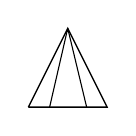
\begin{tikzpicture}[x=1mm,y=1mm]
\draw[line width=.5pt] (0,0)--(5,10)--(10,0)--(0,0);
\draw[line width=.4pt] (5,10)--(2.7,0) (5,10)--(7.4,0);
\end{tikzpicture}}}
\end{GelfandAdjacentEvidence}

$\mathfrak g$ ест. действует, $S$ порожд. ими и подобиями



\begin{GelfandAdjacentEvidence}{GELFAND-P000216}{4}
[Зачёркнуто: растя... / растяже...?]
\Incomplete{GELFAND-P000216}{cancelled-dilation}{Перед «сжатиями» зачёркнуто слово или начало слова; различимо начало «раст...». Окончание не установлено.}
\end{GelfandAdjacentEvidence}

сжатиями к вершине (и в точку).



\underline{Аксиомы.}



$1^{\circ}$. $T$ стягиваемо преобразованиями из $S$ в отмеч. точку $\ast$.



$2^{\circ}$. $\mathfrak g$ замкн. в группе всех гомеом. $T$ в себя.



$3^{\circ}$. $\ast$ неподвижна отн. всех преобр. из $S$.



$4^{\circ}$. $\varphi_t:T\longrightarrow T$



\begin{GelfandAdjacentEvidence}{GELFAND-P000216}{5}
\begin{equation*}\begin{gathered}\varphi_0=\text{тожд.},\quad\varphi_t\in S\quad\text{---}\\\varphi_1(T)=\ast\end{gathered}\end{equation*}
\Unclear{GELFAND-P000216}{axiom-four-homotopy}{Греческий знак отображений имеет расходящиеся верхние штрихи и ножку: $\varphi$ / $\psi$. В четвёртой аксиоме и следующей фразе кандидат $\varphi$; точная буква не установлена. Индексы $0$, $t$, $1$, тождественность и образ $\ast$ читаются.}
\end{GelfandAdjacentEvidence}

--- гомотопия аксиомы $1^{\circ}$.



Тогда сущ. $\varphi_t$, такие что $\varphi_t$ при $t<1$ топологич. вложения.



$5^{\circ}$. $S$ содержит все преобр. $\mathfrak g$ и отображения,
близкие к отобр. $\mathfrak g$ в $S$, суть топ. вложения.



$U(1)\subset S$ сост. из вложений.



\begin{GelfandAdjacentEvidence}{GELFAND-P000216}{6}
В этой ситуации опред. пр-ва






\SourceFigure{GELFAND-P000216}{universal-map}{\par\smallskip\centering{\color{black}\(\displaystyle \begin{tikzcd}[ampersand replacement=\&]\mathcal E_{\mathfrak g}\arrow[d]\\S_{\mathfrak g}\end{tikzcd}\)


, действие $\mathfrak g$ на $\mathcal E_{\mathfrak g}$ --- универс. главное рассл.
}}
\end{GelfandAdjacentEvidence}





\begin{equation*}\underbrace{T\times\cdots\times T}_{I\text{ раз}}\qquad\text{тих. топология.}\end{equation*}



\begin{GelfandAdjacentEvidence}{GELFAND-P000216}{7}
$6^{\circ}$. $\mathfrak g$ действует эффективно на $T$,



(иначе [удвл. / удовл.?] точка)
\Unclear{GELFAND-P000216}{final-abbreviation}{В последней скобке сокращение «удвл.» / «удовл.». Чтение и развёртывание слова не установлены.}
\end{GelfandAdjacentEvidence}



\begin{GelfandAdjacentEvidence}{GELFAND-P000217}{1}
\SourcePage{GELFAND-P000217}{unlabelled}
Элемент $\mathcal E_{\mathfrak g}$ --- всякое вложение $T\subset T^I$, такое
что композиции его со всеми проекциями лежит в $S$.
\Unclear{GELFAND-P000217}{group-letter}{В индексе у округлой E и далее в $C\mathfrak g$, действии и когомологиях петлеобразный групповой знак: $\mathfrak g$ / рукописное прописное $G$. Кандидат $\mathfrak g$; регистр не установлен.}
\end{GelfandAdjacentEvidence}

1) $T=\mathbb R^n$ --- все $n$-реперы.



2) $T=C\mathfrak g$, $\mathcal E_{\mathfrak g}=C\mathfrak g\times\ldots\times C\mathfrak g\setminus\{\ast,\ldots,\ast\}$.



$\mathfrak g$ действует в $\mathcal E_{\mathfrak g}$ домножением на преобр. из $\mathfrak g$.



\begin{GelfandAdjacentEvidence}{GELFAND-P000217}{2}
\begin{equation*}
I\text{ конечно}\quad\Rightarrow\quad
\begin{aligned}
&1)\ \text{обычное классиф. пр-во}\\
&2)\ \text{констр. Милнора с не очень сущ. изменением.}
\end{aligned}
\end{equation*}







\SourceFigure{GELFAND-P000217}{ray-example}{\par\smallskip\centering{\color{black}$\mathfrak g=\mathbb R$, $T={}$
\begin{tikzpicture}[baseline=-0.5ex]
\draw (0,0)--(1.6,0);
\fill (0,0) circle (1.5pt);
\end{tikzpicture}}}
\end{GelfandAdjacentEvidence}

$\mathcal E_{\mathfrak g}$ --- послед. неотр. чисел.



\begin{GelfandAdjacentEvidence}{GELFAND-P000217}{3}
Для каждого $T$ своё опред. лок. тривиальности.







\SourceFigure{GELFAND-P000217}{principal-diagram}{\par\smallskip\centering{\color{black}\begin{tikzcd}[row sep=small,ampersand replacement=\&]
E \arrow[d,"\mathfrak g"]\\ X
\end{tikzcd}}}
\end{GelfandAdjacentEvidence}
\begin{GelfandAdjacentEvidence}{GELFAND-P000217}{4}

лок. трив., если индуц. рассл.







\SourceFigure{GELFAND-P000217}{induced-diagram}{\par\smallskip\centering{\color{black}\begin{tikzcd}[row sep=small,ampersand replacement=\&]
E^{\#} \arrow[d,"T"]\\ X
\end{tikzcd}}}
, облад. св-вом:
$\forall x\ \exists$ отобр. $E^{\#}\longrightarrow T$, гомеом. на слое над $x$ и
$\forall$ слое есть преобр. из $S$.




\end{GelfandAdjacentEvidence}
\underline{Теорема.}



Всякое расслоение отображается в это.



($X$ --- все хаусдорфовы)



Определено $H^q_{\mathrm{alg}}(\mathfrak g;\mathbb R)$



\underline{Теорема.}



Каковы бы ни были $T$ и $S$ $H^q_{\mathrm{alg}}(\mathfrak g,\mathbb R)$
не зависит от их выбора



(Вместо $\mathbb R$ можно брать группу $A$)



\underline{Что будет?}



Успенский, Лекции по логике 2



Лидский, Асимптотика соб. ф-й (по Hörmander'у)



Синай, Условия на диффеом., при к-рых есть инвар. мера



Каждан, Дискр. группы --- решение пробл. Сельберга



Кушниренко, Аналит. действие полупр. группы в окр. неподв. точки --- линейно







\SourcePage{GELFAND-P000218}{7}
Тюрина и С. Гельфанд\quad обзор работ Фама.

Аносов и Маслов

И. Бернштейн\quad $P^{\lambda}$

Гельфанд, Граев

\begin{GelfandAdjacentEvidence}{GELFAND-P000218}{1}
С. Г. Крейн\quad \Unclear{GELFAND-P000218}{list-interpolation}{Интерполяции / Интерполяция}
\end{GelfandAdjacentEvidence}


$\begin{gathered}\text{Березин}\\\text{Кириллов}\end{gathered}$,\quad Грассманов анализ.

\begin{center}
$\text{—}\,\bullet\,\text{—}$
\end{center}





\begin{GelfandAdjacentEvidence}{GELFAND-P000219}{1}
\SourcePage{GELFAND-P000219}{unlabelled}
$16/\underline{\overline{\mathrm{X}}}$\quad \Unclear{GELFAND-P000219}{heading-cancelled}{[Зачёркнуто: неразборчиво.]}
\end{GelfandAdjacentEvidence}
\quad \underline{С. Г. Крейн.}

\begin{GelfandAdjacentEvidence}{GELFAND-P000219}{2}
\underline{Об интерполяции линейных операторов.}






\SourceFigure{GELFAND-P000219}{endpoint-map}{\par\smallskip\centering{\color{black}\(\displaystyle 
\left.
\begin{aligned}
 E_0,\ &\overset{A}{\longrightarrow}\ F_0,\\
 E_1,\ &\overset{A}{\longrightarrow}\ F_1,
\end{aligned}
\right\}\quad\text{банаховы пр-ва,}
\)}}
\end{GelfandAdjacentEvidence}
\begin{GelfandAdjacentEvidence}{GELFAND-P000219}{3}

\Unclear{GELFAND-P000219}{upper-embedding}{все вложенные / все вложены}
\end{GelfandAdjacentEvidence}
 в одно Т.Л.П. (левые и правые)

$A$ ограничен.

$E$, $F$ — интерпол. пара, если $\forall\ A$ из огранич.
при $0$ и $1$ следует огр. $A:E\longrightarrow F$.



Все пр-ва будут пр-вами суммир. функций.



\begin{GelfandAdjacentEvidence}{GELFAND-P000219}{4}
Банахово пр-во сумм. ф-й [Вписано под строкой: на $[0,1]$.]
\Unclear{GELFAND-P000219}{definition-abbreviation}{на / наз.}
\end{GelfandAdjacentEvidence}
 симметрическим, если

1) $y(t)\in E$
\begin{equation*}
 |x(t)|\leq |y(t)|\quad\Longrightarrow\quad x\in E
 \qquad\text{и}\qquad \|x\|\leq\|y\|
\end{equation*}



2) Норма не меняется при преобр., сохр. меру
(можно рассм. равноизмеримую монотонную)



Тогда $L_\infty\subset E\subset L_1$.



\begin{GelfandAdjacentEvidence}{GELFAND-P000219}{5}
\underline{Примеры.} 1)
\begin{equation*}
 \int_0^1 x^*(t)\,d\psi(t),\qquad \psi(t)\text{ — монот.}
 \qquad\text{— }\underline{\text{типа Лоренца}}
\end{equation*}
\Unclear{GELFAND-P000219}{lorentz-example}{В дифференциале, подписи о монотонности и знаменателе следующего примера трёхлучевой греческий знак с нижним штрихом: $\psi$ / $\Psi$. Кандидат $\psi$; регистр не установлен.}
\end{GelfandAdjacentEvidence}

$x^*(t)$ — перестановка $|x(t)|$



2) Двойств.\quad
$\displaystyle\sup_e\frac{\int_e|x(t)|\,dt}{\psi(me)}$



3) и пр-ва Орлич (в них входят $L_p$)



[Слева над строкой:] 1-й шаг.

Теор. Рисса-Торина.





\SourcePage{GELFAND-P000220}{unlabelled}
2-й шаг.

Теор. Марцинкевича.

(На концах треб. меньше)



\begin{equation*}
 n_x(\tau)=\operatorname{mes}\{t:|x(t)|\geq\tau\}
\end{equation*}



\begin{equation*}
 [n_{Ax}(\tau)]^{1/q_i}\leq\frac{C}{\tau}\|x\|_{L_{p_i}}
\end{equation*}
— менее огр. условие.



Большинство опер. анализа на концах удовл. усл. Марцинкевича



\underline{Мацаев и Дикарев} — точнее из $L_p$ в более узкое, чем $L_q$
пр-во (типа Лоренца)! — и оно уже минимально (посередине)



(Минимален для \underline{всех} операторов
в условиях как Марцинкевича и Рисса-Торина) —



— это для улучшающих операторов:
\begin{equation*}
\begin{gathered}q_1>p_1\\q_2>p_2\end{gathered}
\quad\Big\Vert\quad\text{— как и теор. Марцинкевича.}
\end{equation*}



$p=q$ — перев. в себя — тогда и все остальные шкалы тоже.



Пусть
$\begin{gathered}L_1\longrightarrow L_1\\L_\infty\longrightarrow L_\infty\end{gathered}$
\quad и $\|A\|\leq1$



\begin{GelfandAdjacentEvidence}{GELFAND-P000220}{1}
Перечислить все \Unclear{GELFAND-P000220}{middle-cancelled}{[Зачёркнуто: неразборчиво.]}
\end{GelfandAdjacentEvidence}
\begin{GelfandAdjacentEvidence}{GELFAND-P000220}{2}
 пр-ва, для к-рых тоже $\|A\|\leq1$.







\SourceFigure{GELFAND-P000220}{diagram-pair}{Назначение и направление дополнительных наклонных штрихов не установлены.\par\smallskip\centering{\color{black}
\begin{tikzpicture}[x=12mm,y=12mm,baseline=0pt]
\draw (-0.5,0.35)--(0.65,0.35)--(0.65,-0.45)--(-0.5,-0.45)--cycle;
\draw[->] (-0.9,0)--(1.05,0);
\draw[->] (0,-0.85)--(0,0.95);
\draw (0.31,-0.21)--(0.78,-0.56);
\node[anchor=west] at (0.92,-0.62) {в себя};
\begin{scope}[shift={(3.7,0)}]
\draw (-0.55,0)--(0,0.58)--(0.5,0)--(0,-0.53)--cycle;
\draw[->] (-0.9,0)--(1.05,0);
\draw[->] (0,-0.67)--(0,1);
\draw (0.12,-0.15)--(0.37,-0.52);
\node[anchor=west] at (0.65,-0.58) {в себя};
\end{scope}
\end{tikzpicture}
}}
\end{GelfandAdjacentEvidence}

[Справа от рисунков:] лин. опер. (2-мерн. случай).

\begin{GelfandAdjacentEvidence}{GELFAND-P000220}{3}
Док., что это все симметрические нормы и только они.
\Unclear{GELFAND-P000220}{linear-2d}{Сокращение «Док.» читается; полная форма глагола не записана. Варианты раскрытия: доказать / доказано.}
\end{GelfandAdjacentEvidence}

Общая теорема — Б. С. Митягин.

Необх. и дост., чтобы пр-во было симметрическим.

(и в $\infty$-мерн. случае)



$L_p\overset{A}{\longrightarrow}L_p$\qquad что тогда?

$p\ne1,\infty$

(случ. Марцинкевича)



\begin{equation*}
 \bigl\Vert\underset{\substack{\vert\\\text{хар. ф-я }e}}{\chi_e}\bigr\Vert_E=\varphi(me).
\end{equation*}



(симметр. опять необходима)



получ. ф-я $\varphi(t)$ — хар-ка пр-ва $E$.



\begin{equation*}
 \ell_E=\underline{\lim}_{t\to0}\frac{\varphi(2t)}{\varphi(t)}
 \qquad
 u_E=\overline{\lim}_{t\to0}\frac{\varphi(2t)}{\varphi(t)}
 \qquad 1\leq\ell_E\leq u_E\leq2
\end{equation*}





\SourcePage{GELFAND-P000221}{9}
Для $L_p$ они оба равны $2^{1/p}$

Огранич. всех таких $A$ в $E$ $\Longleftrightarrow$ $1<\ell_E\leq u_E<2$

(1-я теор. Семёнова)



\begin{GelfandAdjacentEvidence}{GELFAND-P000221}{1}
Теор. Митягина не обобщена.
\begin{equation*}
 L_{1/\alpha}\longrightarrow L_{1/\alpha-\Delta}
\end{equation*}
\Unclear{GELFAND-P000221}{upper-target-exponent}{Индекс справа записан диагональной дробью без скобок: $1/\alpha-\Delta$ / $1/(\alpha-\Delta)$. Группировка не установлена.}
\end{GelfandAdjacentEvidence}

$0<\Delta\leq\alpha_0<\alpha<\alpha_1$.



Как перечислить пр-ва, в к-рых опер. такого типа огранич.?



\begin{equation*}
 2^{\alpha_0}<\ell_E\leq u_E<2^{\alpha_1}\quad\Longrightarrow\quad E\longrightarrow E_\Delta,
\end{equation*}



\begin{GelfandAdjacentEvidence}{GELFAND-P000221}{2}
где \Unclear{GELFAND-P000221}{after-where-cancelled}{После «где» два густых коротких знака; точное чтение и наличие зачёркивания не установлены.}
\end{GelfandAdjacentEvidence}

\begin{equation*}
 \|x\|_{E_\Delta}=\|x^*(t)t^{-\Delta}\|_E
\end{equation*}
(Это обобщ. теор. Дикарева и Мацаева — лучшее пр-во)



\begin{GelfandAdjacentEvidence}{GELFAND-P000221}{3}
\underline{Прилож.:}\quad нер. Хаусдорфа-Юнга
\begin{equation*}
 \sqrt[p]{|c_k|^p}\leq\|x\|_{L_p}\qquad\text{— из теор. Рисса}
\end{equation*}
\Unclear{GELFAND-P000221}{hausdorff-formula}{Под первым корнем видны $|c_k|^p$; отдельный знак суммы не различим. У корня показатель $p$, справа норма в $L_p$.}
\end{GelfandAdjacentEvidence}

нер-во Пойа:
\begin{equation*}
 \sqrt[p]{\sum k^{p-2}c_k^{*p}}\leq C\|x\|_{L_p}
\end{equation*}



$c_k^*$ — монот. перест. $|\ |$ коэфф.



Для монот. убыв. коэфф. Фурье — двустор. нер-ва (Харди-Литлвуд)



Между $L_1$ и $L_{1,5}$ нет гильб. интерпол. пр-ва (Семёнов)



\underline{Вопр. Гельфанда:} абстр. описание интерпол. пр-в.
(неизв., пр-ва ли они ф-й.)



\underline{Я. Синай.}

\begin{GelfandAdjacentEvidence}{GELFAND-P000221}{4}
\underline{Построение инвар. мер гладких отобр.}\quad\underline{Марковские разб.}





\SourceFigure{GELFAND-P000221}{torus-cell}{\par\smallskip\centering{\color{black}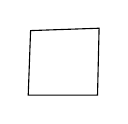
\begin{tikzpicture}
\draw (0,0)--(0.03,0.82)--(0.9,0.85)--(0.88,0)--cycle;
\end{tikzpicture}\par\smallskip
$T(x_1,x_2)=(ax_1+bx_2,\ cx_1+dx_2)$ — отобр. тора
}}
\end{GelfandAdjacentEvidence}

и $T_1$. — другое.

\begin{GelfandAdjacentEvidence}{GELFAND-P000221}{5}
Когда сущ. измеримое отобр. тора, $M\overset{U}{\longrightarrow}M$,
что $UT_1=T_2U$.
\Unclear{GELFAND-P000221}{torus-map-indices}{Сначала $T$, затем $T_1$, в равенстве $T_1$ и $T_2$. Знак у стрелки и по обе стороны равенства петлеобразный: $U$ / $u$; кандидат $U$, регистр не установлен.}
\end{GelfandAdjacentEvidence}

Иррац. соб. знач. $\Rightarrow$ веществ. $\Rightarrow$ эргодично, спектр
счётнокр. лебеговский.



Энтропия $h(T)=\ln\lambda$\quad $(\lambda>1)$





\SourcePage{GELFAND-P000222}{unlabelled}
Если $h$ совп., то ещё не линейно сопряж. (есть другие-инв.)

Но метрически они подобны! ($U$ — разрывное, но измеримое)

\begin{GelfandAdjacentEvidence}{GELFAND-P000222}{1}
$U$ — гомеом. $\Longrightarrow$ он линеен (можно док.)
(для любых комп. аб. групп)
\Unclear{GELFAND-P000222}{top-conjugacy}{Петлеобразный знак отображения в обеих строках: $U$ / $u$. Кандидат $U$; регистр не установлен.}
\end{GelfandAdjacentEvidence}

$\Omega_\Pi$ — пр-во послед. $\omega=\{i_n\}$ — беск. в обе стороны послед.

$i_n\in\{1,\ldots,S\}$



\begin{equation*}
 \underset{\text{порядка }S}{\Pi}=\|x_{ij}\|,\quad x_{ij}=1,0
 \qquad \pi_{i_n i_{n+1}}=1
\end{equation*}
(только такие послед. $\omega$ допуст.)



Будем считать, что $\Pi^k$ — из полож. элем.

Рассм. сдвиг (преобр. сдвига на $\Omega$).



\begin{GelfandAdjacentEvidence}{GELFAND-P000222}{2}
\underline{Пример.}\quad
$\begin{pmatrix}1&0\\0&1\end{pmatrix}$ — не уд. усл., но $\Omega$ — послед.
только из $1$ или \Unclear{GELFAND-P000222}{identity-example-cancelled}{[Зачёркнутый знак: неразборчиво.]}
\end{GelfandAdjacentEvidence}
 только из $2$



$\begin{pmatrix}1&1\\1&1\end{pmatrix}$ — всё можно ставить



$\begin{pmatrix}1&1\\1&0\end{pmatrix}$ — посмотреть.



\begin{GelfandAdjacentEvidence}{GELFAND-P000222}{3}
на $\Omega_\Pi$ задать бы инв. меру $\mu$ с $\max$ энтропией:



\Unclear{GELFAND-P000222}{before-entropy-cancelled}{[Слева от формулы зачёркнутая неразборчивая запись.]}
\end{GelfandAdjacentEvidence}
\begin{GelfandAdjacentEvidence}{GELFAND-P000222}{4}

\begin{equation*}
 h=\max_\mu h_\mu(T)
\end{equation*}
(\Unclear{GELFAND-P000222}{shift-parenthesis-cancelled}{[Зачёркнуто: где / сдв.]}
\end{GelfandAdjacentEvidence}
 $T$ — это сдвиг).

Надо рассмотреть $e$ с полож. коорд.\quad $\lambda e=\Pi^*e$, $\lambda>0$

(единств.)



( Г. Если все элем. и все миноры 2-го порядка $>0$, то
сущ. 2 соб. вектора, 1-й с полож. элем., 2-й — с
1-й переменой знака —

— матр. миноров 2-го пор. — предст. самой матр. во внешнем произв.)



Рассм. цепь Маркова с вер. $\displaystyle p_{ij}=\frac{e_j\pi_{ij}}{\lambda e_i}$ —

[Справа:] — энтроп. — $\ln\lambda$



\begin{equation*}
\left[
\begin{gathered}
\text{Вообще энтр. цепи Маркова}\\
 h=\sum_i e_i\left(-\sum_j\ln p_{ij}\,p_{ij}\right)
\end{gathered}
\right.
\end{equation*}



мера с $\max$ энтропией единственна.



Мера в $\Omega_\Pi$ на $\Sigma$-алг., порожд. цилиндрич. мн-вами.





\SourcePage{GELFAND-P000223}{10}
а) $\{a_1^1,\ldots,a_p^1;\ a_1^2,\ldots,a_q^2;\ b_1^1,\ldots,b_r^1;\ b_1^2,\ldots,b_s^2\}$



\begin{GelfandAdjacentEvidence}{GELFAND-P000223}{1}
$\Pi$
\begin{equation*}
 \text{из }\left.\begin{gathered}\alpha^1\\\alpha^2\end{gathered}\right\}
 \longrightarrow\alpha^1\text{ или }B^1
\end{equation*}
\begin{equation*}
 \text{из }\left.\begin{gathered}\beta^1\\\beta^2\end{gathered}\right\}
 \longrightarrow\alpha^2\text{ или }B^2
\end{equation*}
\Unclear{GELFAND-P000223}{alphabet-type-letters}{В переходах начертания $\alpha/a/A$ и $\beta/b/B$ не установлены однозначно; справа B-подобные знаки крупнее. В алфавите выше $a$ и $b$. В отображённой записи кандидаты $\alpha,\beta$ слева и $B$ справа.}
\end{GelfandAdjacentEvidence}

[На правом поле:] $\Vert$\quad строится по целоч. матр. 2-го пор. разбиение.



\begin{equation*}
\lambda^2-(p+s)\lambda+(ps-qr)=0,\qquad
\begin{gathered}\boxed{\boxed{ps-qr=1}}\\\text{условие.}\end{gathered}
\end{equation*}



б) $\Omega_{\Pi_1}$\qquad $\pi_{ij}=1$ и $\pi_{N1}=0$ (только на 1-м месте)



\underline{\underline{Предл.}}\quad\underline{Сдвиги в а) и б) изоморфны.}



\begin{equation*}
\left[\begin{gathered}
\text{Теперь всё свод. к док-ву того, что}\\
\text{алгебр. автоморфизм }\Rightarrow\\
\Rightarrow\text{ разбиение.}
\end{gathered}\right.
\end{equation*}



Док-во предл.

Алфавит б): $A_1,\ldots,A_p$,\quad $B_1,\ldots,B_s$.



(Изоморфизм любых 2-х $\Omega_\Pi$ с одинаков. энтропией).



Кодируются разные группы (с пом. символов $A_i,B_i$).



Пр-во с 1-й $\max$ мерой перех. в пр-во с другой $\max$ мерой.



\underline{След. раз:} Марк. разбиения и как с их помощью строятся инв. меры.



$23/\underline{\overline{\mathrm{X}}}$.\quad \underline{\underline{Лерэ}}.
\quad\underline{Особенности фейнмановских интегралов.}



N. Nilsson, Arkiv för Math. (Swede)\quad 1964–1965

\begin{GelfandAdjacentEvidence}{GELFAND-P000223}{2}
(уч. Гординга)



\Incomplete{GELFAND-P000223}{lower-crossed-formula}{Под «(уч. Гординга)» зачёркнута короткая формула. Возможное начало $J(\ldots)$; остальные символы неразборчивы.}
\end{GelfandAdjacentEvidence}
\begin{GelfandAdjacentEvidence}{GELFAND-P000223}{3}

\Unclear{GELFAND-P000223}{lower-crossed-symbol}{Отдельный зачёркнутый знак под формулой: $J$ / $\gamma$; чтение не установлено.}
\end{GelfandAdjacentEvidence}
\begin{GelfandAdjacentEvidence}{GELFAND-P000223}{4}





\Unclear{GELFAND-P000223}{integral-annotated}{У цикла надстрочный знак $q$ / $a$; кандидат $q$. Координатный знак в аргументе $\omega$ и ниже: $\xi$ / $\zeta$; кандидат $\xi$. Надписи «цикл относит $W(t)$», «однор. степ. $0$» и «$=0$ на $W(t)$» читаются.\par\smallskip\centering{\color{black}
\begin{tikzpicture}[x=10mm,y=10mm,baseline=0pt]
\node[anchor=base] at (0,0) {$J(t)=$};
\node[anchor=base] at (1.15,0) {$\displaystyle\int_{\gamma^q(t)}$};
\node[anchor=base] at (2.65,0) {$\omega(t,\xi)$};
\draw (1.05,-0.78)--(1.30,-1.00);
\node[anchor=north] at (1.30,-1.10) {цикл};
\node[anchor=north] at (1.30,-1.50) {относит $W(t)$};
\draw (3.00,-0.18)--(3.00,-0.95);
\node[anchor=north] at (4.20,-1.10) {однор. степ. $0$};
\node[anchor=north] at (4.20,-1.50) {$=0$ на $W(t)$};
\end{tikzpicture}
}}
\end{GelfandAdjacentEvidence}

$t\in T=C^n$,

$\xi\in C^{\ell+1}$



$\omega(t,\xi)$ на $P^\ell$, т.к. однородна; там и цикл.





\SourcePage{GELFAND-P000224}{unlabelled}
$W(t)=\bigcup_k W_k(t)$ — гиперплоск., алгебр. ф-и $t$, могут быть особенности (не в общем положении)



$t\in S_0[W]\Longleftrightarrow$ в ней измен. размерность пересеч. любого числа.



\begin{GelfandAdjacentEvidence}{GELFAND-P000224}{1}
Def:
\begin{equation*}
 \gamma^{q-m}(t)=\bigcap_{j=1}^m V_j(t),
\end{equation*}
\Unclear{GELFAND-P000224}{intersection-sign}{Крупный знак: $\bigcap$ / $\bigwedge$; отображён кандидат $\bigcap$.}
\end{GelfandAdjacentEvidence}

\begin{center}
\begin{tikzpicture}[x=10mm,y=10mm,baseline=0pt]
\node[anchor=base] at (2.3,0) {$V_j(t)=v_j(t,x)=0$};
\draw (3.15,-0.32) .. controls (3.20,-0.40) and (3.24,-0.47) .. (3.18,-0.57);
\node[anchor=north] at (3.2,-0.72) {алгебр. мн-ие};
\end{tikzpicture}
\end{center}



\begin{GelfandAdjacentEvidence}{GELFAND-P000224}{2}

Надо предпол.
\begin{equation*}
 \frac{\omega(t,\xi)}{[v_1(t,\xi)]^{1+\beta_1}\ldots[v_m]^{1+\beta_m}}
 \qquad\text{— опред. на }P
\end{equation*}
\Unclear{GELFAND-P000224}{projective-rational-form}{Координатные знаки в аргументе $\omega$ и в первом знаменателе: $\xi$ / $s$; отображён кандидат $\xi$. В последнем множителе написано $[v_m]^{1+\beta_m}$.}
\end{GelfandAdjacentEvidence}
\begin{GelfandAdjacentEvidence}{GELFAND-P000224}{3}

[Слева:] Вычет
\begin{equation*}
 J(t)=\int_{\gamma^{q-m}(\xi)}
 \frac{d^{\beta_1+\ldots+\beta_m}\omega}
 {[dv_1]^{1+\beta_1}\wedge\ldots\wedge[dv_m]^{1+\beta_m}}
\end{equation*}
\Unclear{GELFAND-P000224}{residue-cycle-argument}{Аргумент под интегралом: $\xi$ / $s$; отображён кандидат $\xi$.}
\end{GelfandAdjacentEvidence}




Особ. носитель в общ. случае тоже описывается

(На накрыв. пр-ве дополнения форма будет голоморфна)



\begin{GelfandAdjacentEvidence}{GELFAND-P000224}{4}
\underline{\underline{Теор.}} Тогда $J(t)$ имеет алгебр. син. носитель.



\Unclear{GELFAND-P000224}{theorem-margin-note}{Приписка справа: «типа ст. алгебр.» / «типа см. алгебр.»; первое слово и среднее сокращение не установлены однозначно.}
\end{GelfandAdjacentEvidence}

(т.е. в $T$ сущ. алг. мн-ие, что $J(t)$ голом. на накр. дополн.)



Лерэ описал син. носит. в случае плоскостей.



$30/\underline{\overline{\mathrm{X}}}$\quad\underline{\underline{Синай.}}
\begin{center}
\begin{tikzpicture}[x=10mm,y=10mm,baseline=0pt]
\node[anchor=base] at (2.6,0) {$U$-диффеом.};
\draw (0,-0.24) .. controls (0.16,-0.10) and (0.35,-0.10) .. (0.52,-0.24)
 .. controls (0.69,-0.38) and (0.87,-0.38) .. (1.04,-0.24)
 .. controls (1.21,-0.10) and (1.39,-0.10) .. (1.56,-0.24)
 .. controls (1.73,-0.38) and (1.91,-0.38) .. (2.08,-0.24)
 .. controls (2.25,-0.10) and (2.43,-0.10) .. (2.60,-0.24)
 .. controls (2.77,-0.38) and (2.95,-0.38) .. (3.12,-0.24)
 .. controls (3.29,-0.10) and (3.47,-0.10) .. (3.64,-0.24)
 .. controls (3.81,-0.38) and (3.99,-0.38) .. (4.16,-0.24)
 .. controls (4.33,-0.10) and (4.51,-0.10) .. (4.68,-0.24)
 .. controls (4.85,-0.38) and (5.03,-0.38) .. (5.20,-0.24);
\end{tikzpicture}
\end{center}




хар. $\exp$ рост расст. между близкими точками (разбегание)

либо при $t\longrightarrow+\infty$, либо при $t\longrightarrow-\infty$.



\begin{equation*}
 \frac{d(T^n x,T^n y)}{d(x,y)}\geq ae^{cn}
 \qquad\begin{gathered}n>0\\\text{или }n<0\end{gathered}
 \qquad(x,y\text{ — близки})
\end{equation*}



Рассм. точки $d(T^n y,T^n x)\leq ae^{-cn}d(y,x)$,



\begin{GelfandAdjacentEvidence}{GELFAND-P000224}{5}
Пусть $\forall\ x$ это $k$-мерное подмн-ие.







\SourceFigure{GELFAND-P000224}{manifold-sketch}{\par\smallskip\centering{\color{black}
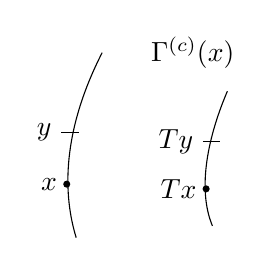
\begin{tikzpicture}[x=10mm,y=10mm]
\draw (0.15,0) .. controls (-0.05,0.65) and (0.02,1.45) .. (0.48,2.35);
\fill (0.03,0.68) circle (0.045);
\node[left] at (0.03,0.68) {$x$};
\draw (-0.04,1.34)--(0.19,1.34);
\node[left] at (-0.04,1.34) {$y$};
\draw (1.88,0.15) .. controls (1.68,0.63) and (1.83,1.3) .. (2.07,1.86);
\fill (1.8,0.62) circle (0.045);
\node[left] at (1.8,0.62) {$Tx$};
\draw (1.76,1.22)--(1.98,1.22);
\node[left] at (1.76,1.22) {$Ty$};
\node at (1.63,2.35) {$\Gamma^{(c)}(x)$};
\end{tikzpicture}
}}
\end{GelfandAdjacentEvidence}

Это сжимающееся подмн-ие (отсюда индекс \underline{\underline{$c$}})



\begin{equation*}
 d(T^n y',T^n x)\leq ae^{+cn}d(y',x)
 \qquad(n\longrightarrow-\infty).
\end{equation*}



Получим подобн. $\Gamma^{(p)}(x)$ — расшир. подмн-ие.

($\ell$-мерное).



Тогда выбор не зав. от $a$ и $c$.





\SourcePage{GELFAND-P000225}{11}
$U$-система:
$k+\ell=n$ и кас. пр-ва к подмн. равном. трансверсальны



1. $k+\ell=n$

2. трансверс.

3. Гладкость (не выпис. явно).



Получаем 2 слоения $\gamma^{(\mathrm{c})}$ и $\gamma^{(\mathrm{p})}$.



\begin{GelfandAdjacentEvidence}{GELFAND-P000225}{1}
\underline{Пример:} лин. преобр. тора
$(x,y)\longrightarrow(ax+by,cx+dy)$.
\begin{equation*}
 \begin{vmatrix}a&b\\c&d\end{vmatrix}=1.
\end{equation*}





\Unclear{GELFAND-P000225}{lattice-diagram}{Две семьи наклонных линий и оси со стрелками вверх и вправо. Число совпадающих линий и продолжения внутри густых пересечений не установлены однозначно. Подписей у отдельных линий нет.\par\smallskip\centering{\color{black}\begin{minipage}{68mm}\centering 
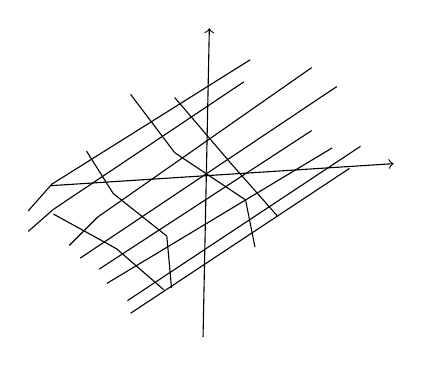
\begin{tikzpicture}[x=0.20mm,y=-0.20mm]
\draw (25,136)--(40,119)--(166,40);
\draw (25,149)--(41,135)--(162,54);
\draw (51,158)--(69,140)--(205,45);
\draw (58,166)--(221,57);
\draw (70,173)--(205,85);
\draw (75,182)--(218,96);
\draw (88,193)--(236,95);
\draw (90,201)--(229,109);
\draw (90,62)--(118,99)--(163,129)--(169,159);
\draw (118,64)--(153,105)--(183,139);
\draw (62,98)--(79,125)--(113,152)--(116,185);
\draw (41,138)--(81,160)--(111,186);
\draw[->] (136,216)--(140,20);
\draw[->] (39,120)--(257,106);
\end{tikzpicture}


(паралл. соб. напр.).
\end{minipage}}}
\end{GelfandAdjacentEvidence}

Нелин. возмущение (периодич. и гладкое) — тоже
$U$-диффеом. и число вращ. то же.



\begin{center}
\begin{tikzpicture}[x=10mm,y=10mm,baseline=0pt]
\node[anchor=base] at (3.6,0) {Метод постр. $U$-дифф.};
\draw (0,-0.24) .. controls (0.2,-0.07) and (0.4,-0.07) .. (0.6,-0.24)
 .. controls (0.8,-0.41) and (1.0,-0.41) .. (1.2,-0.24)
 .. controls (1.4,-0.07) and (1.6,-0.07) .. (1.8,-0.24)
 .. controls (2.0,-0.41) and (2.2,-0.41) .. (2.4,-0.24)
 .. controls (2.6,-0.07) and (2.8,-0.07) .. (3.0,-0.24)
 .. controls (3.2,-0.41) and (3.4,-0.41) .. (3.6,-0.24)
 .. controls (3.8,-0.07) and (4.0,-0.07) .. (4.2,-0.24)
 .. controls (4.4,-0.41) and (4.6,-0.41) .. (4.8,-0.24)
 .. controls (5.0,-0.07) and (5.2,-0.07) .. (5.4,-0.24)
 .. controls (5.6,-0.41) and (5.8,-0.41) .. (6.0,-0.24)
 .. controls (6.2,-0.07) and (6.4,-0.07) .. (6.6,-0.24)
 .. controls (6.8,-0.41) and (7.0,-0.41) .. (7.2,-0.24);
\end{tikzpicture}
\end{center}




$g$ — гр. Ли, $\Gamma$ — дискр. подгр.

\begin{GelfandAdjacentEvidence}{GELFAND-P000225}{2}
$g/\Gamma$ — компактна.
\Unclear{GELFAND-P000225}{group-notation}{Обозначение группы Ли: $g$ / $\mathfrak{G}$; отображён кандидат $g$, отдельный от последующего $G$.}
\end{GelfandAdjacentEvidence}

\begin{tikzpicture}[x=10mm,y=10mm,baseline=(symbol.base)]
\node (symbol) at (0,0) {$T_{\mathrm{alg}}$};
\draw (-0.45,-0.28) .. controls (-0.45,-0.60) and (0.50,-0.60) .. (0.80,-0.28);
\node[anchor=north,align=center,text width=35mm] at (0.15,-0.70) {автом. как группы};
\end{tikzpicture}
 — алг. автом. $g$, ост. неподв. $\Gamma$
\quad$(T_{\mathrm{alg}}\Gamma=\Gamma)$



Тогда он действ. на $g/\Gamma$.



Рассм. $G$ — алгебру Ли; $\hat T_{\mathrm{alg}}$ — соотв. автом. $G$; если его

[У левого края следующей строки:] соб. знач.



\begin{GelfandAdjacentEvidence}{GELFAND-P000225}{3}
Среди них нет
\Unclear{GELFAND-P000225}{cancelled-before-eigenvalues}{Зачёркнуто: $\Longleftrightarrow$ / $\Longrightarrow$; направления концов не установлены.}
\end{GelfandAdjacentEvidence}
\begin{GelfandAdjacentEvidence}{GELFAND-P000225}{4}

соб. знач. $=1$ по $\operatorname{mod}$



\Unclear{GELFAND-P000225}{terminal-arrow}{Знак после mod: $\Leftrightarrow$ / зачёркнутый знак.}
\end{GelfandAdjacentEvidence}

$\Longleftrightarrow$ это $U$-диффеом.



\begin{GelfandAdjacentEvidence}{GELFAND-P000225}{5}
(Существуют $\Longleftrightarrow G$ нильпотентна).
\Unclear{GELFAND-P000225}{nilpotence-parenthesis}{Начальное слово в скобках: «Существуют» / «Существует»; отображён первый кандидат. Вся скобка приведена в оригинальном фрагменте.}
\end{GelfandAdjacentEvidence}

Дальше. Малое нелин. возмущение $T=T_{\mathrm{alg}}+\Delta T$ — тоже $U$-дифф.



\underline{Осн. проблема:} топ. подобность алгебраич.



Для малых возмущ. — из общей теор. Аносова

(Малое возм. $U$-дифф. топ. подобно исходному).



Всегда.
\begin{equation*}
 M=M_1\cup M_2
\end{equation*}



$M_2$ — блужд. точки



$M_1$ — неблужд. точки. — на них вып. условие $U$



[На правом поле:]
\begin{center}
\begin{tikzpicture}[x=10mm,y=10mm]
\draw (0,0)--(0,0.85);
\node[anchor=west,align=left] at (0.2,0.43) {тоже\\гипотеза};
\end{tikzpicture}
\end{center}






\begin{GelfandAdjacentEvidence}{GELFAND-P000226}{1}
\SourcePage{GELFAND-P000226}{unlabelled}
Важное построение:







\SourceFigure{GELFAND-P000226}{holonomy-diagram}{\par\smallskip\centering{\color{black}
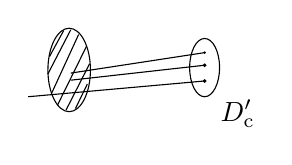
\begin{tikzpicture}[x=10mm,y=10mm]
\draw (0,0) ellipse (0.27 and 0.53);
\draw (-0.22,-0.29)--(0.12,0.45);
\draw (-0.27,-0.05)--(0.02,0.51);
\draw (-0.25,0.17)--(-0.07,0.50);
\draw (-0.15,-0.45)--(0.22,0.30);
\draw (-0.04,-0.51)--(0.26,0.08);
\draw (0.08,-0.49)--(0.23,-0.18);
\draw (1.72,0.03) ellipse (0.19 and 0.37);
\draw (0.02,-0.04)--(1.72,0.22);
\draw (0.02,-0.13)--(1.72,0.06);
\draw (-0.52,-0.34)--(1.72,-0.14);
\fill (1.72,0.22) circle (0.018);
\fill (1.72,0.06) circle (0.025);
\fill (1.72,-0.14) circle (0.025);
\node[below right] at (1.80,-0.26) {$D'_{\mathrm{c}}$};
\end{tikzpicture}
}}
\end{GelfandAdjacentEvidence}

естеств. изом. наших кусочков. сжим. слоёв (по несжим. слоям).



$D_{\mathrm{c}}$ — сжим. подмн. $\dim=k$.



($\pi$ — канон. изом.)



\begin{GelfandAdjacentEvidence}{GELFAND-P000226}{2}
$\pi$ не всегда гладко (!), но оно абс. непр., т. е. естеств. меры перев. друг. в друга.





\Unclear{GELFAND-P000226}{parallelogram-diagram}{Два почти вертикальных кривых штриха и поперечные кривые; в густых средних пересечениях число совпадающих штрихов и их продолжения не установлены однозначно. Подписей и стрелок не видно.\par\smallskip\centering{\color{black}\begin{minipage}{68mm}\centering Параллелограмм:
\begin{center}
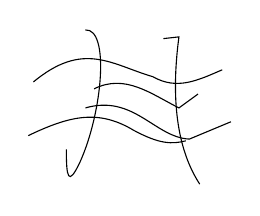
\begin{tikzpicture}[x=0.22mm,y=-0.22mm]
\draw (80,28) .. controls (94,27) and (90,75) .. (77,104)
 .. controls (70,119) and (69,113) .. (69,97);
\draw (125,33)--(134,32) .. controls (130,62) and (131,94) .. (146,117);
\draw (50,58) .. controls (79,34) and (95,48) .. (119,55)
 .. controls (133,63) and (145,57) .. (159,51);
\draw (85,62) .. controls (103,53) and (118,65) .. (134,73)--(145,65);
\draw (80,73) .. controls (108,65) and (120,90) .. (140,91)--(164,81);
\draw (47,89) .. controls (72,77) and (88,74) .. (108,86)
 .. controls (123,94) and (130,94) .. (138,92);
\end{tikzpicture}
\end{center}

из отрезков слоений
\end{minipage}}}
\end{GelfandAdjacentEvidence}

(все принадл. ему слои кан. изоморфны: и сжим. и расшир.)



\begin{equation*}
 \Gamma(U)=\Gamma_{\mathrm{p}}(U)\cup\Gamma_{\mathrm{c}}(U)
\end{equation*}



Пусть есть система паралл. $U_i$, примык. друг к другу.



\begin{equation*}
 \begin{gathered}
 M=\bigcup\overline{U}_i\\
 U_i\cap U_j\subset\Gamma(U_i)\cap\Gamma(U_j)
 \end{gathered}
 \qquad(\Gamma\text{ — границы}).
\end{equation*}



$\alpha$ — такое разб. на пар-мы. Рассм. границы:



\begin{equation*}
 \begin{gathered}
 \Gamma_{\mathrm{p}}(\alpha)=\bigcup_i\Gamma_{\mathrm{p}}(U_i)\\
 \Gamma_{\mathrm{c}}(\alpha)=\bigcup_i\Gamma_{\mathrm{c}}(U_i)
 \end{gathered}
\end{equation*}



\begin{GelfandAdjacentEvidence}{GELFAND-P000226}{3}
[Справа рисунок:]




\SourceFigure{GELFAND-P000226}{boundary-diagram}{\par\smallskip\centering{\color{black}
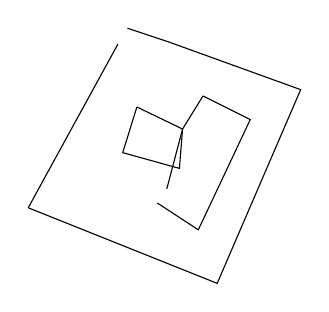
\begin{tikzpicture}[x=0.20mm,y=-0.20mm]
\draw (25,142)--(82,38);
\draw (88,28)--(115,37)--(198,67)--(145,190)--(25,142);
\draw (136,71)--(166,86)--(133,156)--(107,139);
\draw (113,130)--(123,92)--(136,71);
\draw (94,78)--(85,107)--(121,117)--(123,92)--(94,78);
\end{tikzpicture}
}}
\end{GelfandAdjacentEvidence}

Это $\alpha$ наз. марковским, если сущ. $m$, такое что



\begin{equation*}
 \fbox{$\begin{gathered}
 \Gamma_{\mathrm{p}}(T^{-m}\alpha)\subset\Gamma_{\mathrm{p}}(\alpha)\\
 \Gamma_{\mathrm{c}}(T^{+m}\alpha)\subset\Gamma_{\mathrm{c}}(\alpha)
 \end{gathered}$}
\end{equation*}



\begin{center}
\begin{tikzpicture}[x=10mm,y=10mm]
\node[anchor=north west,align=left,text width=126mm,inner sep=2mm] (statement) at (0,0) {\underline{Теор.} (технич.) Марк. разб. сущ. и их много: $\forall$ \begin{tikzpicture}[x=10mm,y=10mm,baseline=(parameter.base)]
\node (parameter) at (0,0) {$\alpha$};
\draw (-0.02,-0.23)--(-0.22,-0.70);
\node[anchor=north,align=center] at (-0.22,-0.78) {разб.\\на пар-мы};
\end{tikzpicture}, $\forall\varepsilon>0$ $\exists m$ и разб. $\widetilde\alpha$, что оно будет отст. от исходного меньше чем на $\varepsilon$.};
\draw (statement.north east)--(statement.north west)--++(-0.35,0)--++(0,-0.45)--++(-0.65,0)--++(0,-1.15)--++(0.65,0) |- (statement.south west)--(statement.south east);
\end{tikzpicture}
\end{center}



\begin{GelfandAdjacentEvidence}{GELFAND-P000226}{4}

[Слева:]




\Unclear{GELFAND-P000226}{bottom-diagrams}{Отдельный наклонный четырёхугольник и узкая наклонная полоса с поперечными четырёхугольниками у концов. Продолжения нескольких наложенных контуров у верхнего правого конца не установлены однозначно. Стрелок нет.\par\smallskip\centering{\color{black}
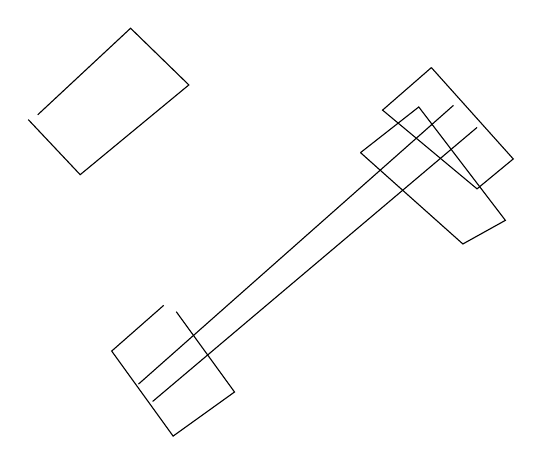
\begin{tikzpicture}[x=0.20mm,y=-0.20mm]
\draw (32,92)--(91,37)--(128,73)--(59,130)--(26,95);
\draw (96,263)--(296,86);
\draw (105,274)--(311,100);
\draw (282,62)--(334,120)--(311,139)--(251,89)--(282,62);
\draw (237,116)--(274,87)--(329,159)--(302,174)--(237,116);
\draw (112,213)--(79,242)--(118,296)--(157,268)--(120,217);
\end{tikzpicture}
}}
\end{GelfandAdjacentEvidence}

концы не могут быть в середине.

(исх. пар.)



\begin{center}$\text{—}\,\bullet\,\text{—}$\end{center}



Если $\alpha$ — разб. с $m$, то можно сделать $m=1$, взяв пересечение



\begin{equation*}
 \alpha_1=\alpha\cdot T^{-1}\alpha\cdots\cdot T^{-m+1}\alpha\;\text{—}
\end{equation*}
— марковское с $m=1$





\SourcePage{GELFAND-P000227}{12}
— из
\begin{equation*}
 \Gamma_{\mathrm{p}}(\alpha_1)=\Gamma_{\mathrm{p}}(\alpha)
 \cup\Gamma_{\mathrm{p}}(T^{-1}\alpha)\cup\cdots
 \cup\Gamma_{\mathrm{p}}(T^{-m+1}\alpha)
\end{equation*}



\begin{center}
\begin{tikzpicture}[x=1mm,y=1mm]
\node[anchor=base,align=left,text width=136mm] at (70.0,0) {Символическая динамика для $U$-диффеом.};
\draw (0,-2) .. controls (2,-1) and (4,-1) .. (6,-2)
 .. controls (8,-3) and (10,-3) .. (12,-2)
 .. controls (14,-1) and (16,-1) .. (18,-2)
 .. controls (20,-3) and (22,-3) .. (24,-2)
 .. controls (26,-1) and (28,-1) .. (30,-2)
 .. controls (32,-3) and (34,-3) .. (36,-2)
 .. controls (38,-1) and (40,-1) .. (42,-2)
 .. controls (44,-3) and (46,-3) .. (48,-2)
 .. controls (50,-1) and (52,-1) .. (54,-2)
 .. controls (56,-3) and (58,-3) .. (60,-2)
 .. controls (62,-1) and (64,-1) .. (66,-2)
 .. controls (68,-3) and (70,-3) .. (72,-2)
 .. controls (74,-1) and (76,-1) .. (78,-2)
 .. controls (80,-3) and (82,-3) .. (84,-2)
 .. controls (86,-1) and (88,-1) .. (90,-2)
 .. controls (92,-3) and (94,-3) .. (96,-2)
 .. controls (98,-1) and (100,-1) .. (102,-2)
 .. controls (104,-3) and (106,-3) .. (108,-2)
 .. controls (110,-1) and (112,-1) .. (114,-2)
 .. controls (116,-3) and (118,-3) .. (120,-2)
 .. controls (122,-1) and (124,-1) .. (126,-2)
 .. controls (128,-3) and (130,-3) .. (132,-2)
 .. controls (134,-1) and (136,-1) .. (138,-2);
\end{tikzpicture}
\end{center}




(Пусть есть марк. разб. и с $m=1$)



\begin{equation*}
 \pi_{j_1j_2}=\begin{cases}
 1&V_{j_1}\cap TV_{j_2}\ne\varnothing\\
 0&\text{в ост. случаях}
 \end{cases}
\end{equation*}
\Needspace{8\baselineskip}
$\Pi$\par\nobreak



$\Omega_\Pi$ — пр-во из точек
\begin{equation*}
 \begin{gathered}
 \omega=\{\ldots\ j_{-n},\ldots,j_0,\ldots,j_n,\ldots\}\\
 \pi_{j_nj_{n+1}}=1.
 \end{gathered}
\end{equation*}



Сопоставим теперь
\begin{equation*}
 \omega\longrightarrow\bigcap_{-\infty}^{+\infty}T^n\overline{V}_{j_n}
 =x\in M\qquad(!)
\end{equation*}



(непусто из марковости и при мелком разб. из 1-й точки)



Получ. отображение $\varphi:\Omega_\Pi\longrightarrow M$



[Справа начата скобка:] (из неединств.



\begin{GelfandAdjacentEvidence}{GELFAND-P000227}{1}
оно не
\Unclear{GELFAND-P000227}{overwritten-negation}{После читаемого «не» зачёркнута короткая запись; возможное «вз.» не установлено.}
\end{GelfandAdjacentEvidence}

вз.-одн. из-за точек — границ пар-мов).

На мн-ве 2-й катег. вз.-однозначно.



\underline{Условие:} $\Pi^K$ из полож. элем. при нек-ром $K$.



(т. е. все слои $\Gamma^{(\mathrm{c})}$ и $\Gamma^{(\mathrm{p})}$ плотны на $M$ — это необх. и достат.)



\begin{center}
\begin{tikzpicture}[x=1mm,y=1mm]
\node[anchor=base,align=left,text width=136mm] at (70.0,0) {На каждом слое $\Gamma^{(\mathrm{c})}$ вводится $\sigma$-конечная мера $\lambda_{\mathrm{c}}$,};
\draw (0,-2) .. controls (2,-1) and (4,-1) .. (6,-2)
 .. controls (8,-3) and (10,-3) .. (12,-2)
 .. controls (14,-1) and (16,-1) .. (18,-2)
 .. controls (20,-3) and (22,-3) .. (24,-2)
 .. controls (26,-1) and (28,-1) .. (30,-2)
 .. controls (32,-3) and (34,-3) .. (36,-2)
 .. controls (38,-1) and (40,-1) .. (42,-2)
 .. controls (44,-3) and (46,-3) .. (48,-2)
 .. controls (50,-1) and (52,-1) .. (54,-2)
 .. controls (56,-3) and (58,-3) .. (60,-2)
 .. controls (62,-1) and (64,-1) .. (66,-2)
 .. controls (68,-3) and (70,-3) .. (72,-2)
 .. controls (74,-1) and (76,-1) .. (78,-2)
 .. controls (80,-3) and (82,-3) .. (84,-2)
 .. controls (86,-1) and (88,-1) .. (90,-2)
 .. controls (92,-3) and (94,-3) .. (96,-2)
 .. controls (98,-1) and (100,-1) .. (102,-2)
 .. controls (104,-3) and (106,-3) .. (108,-2)
 .. controls (110,-1) and (112,-1) .. (114,-2)
 .. controls (116,-3) and (118,-3) .. (120,-2)
 .. controls (122,-1) and (124,-1) .. (126,-2)
 .. controls (128,-3) and (130,-3) .. (132,-2)
 .. controls (134,-1) and (136,-1) .. (138,-2);
\end{tikzpicture}
\end{center}

\begin{GelfandAdjacentEvidence}{GELFAND-P000227}{2}
причем

[Слева:]




\Unclear{GELFAND-P000227}{invariant-measure-diagram}{Линии с $A,\widetilde A$ и соединяющие их кривые. У двух нижних правых концов видны направленные утолщения; число совпадающих нижних кривых и характер остальных концов не установлены однозначно.\par\smallskip\centering{\color{black}
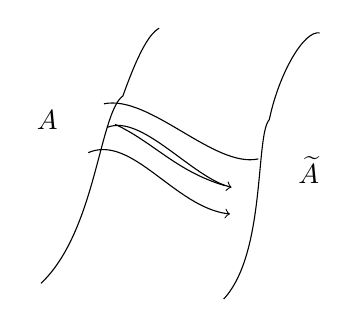
\begin{tikzpicture}[x=0.20mm,y=-0.20mm]
\draw (30,194) .. controls (65,161) and (67,86) .. (82,75)
 .. controls (91,50) and (98,36) .. (105,32);
\draw (146,204) .. controls (173,175) and (166,100) .. (175,90)
 .. controls (181,61) and (197,33) .. (207,35);
\node at (34,90) {$A$};
\node at (200,122) {$\widetilde A$};
\draw (70,80) .. controls (99,74) and (140,121) .. (168,115);
\draw[->] (72,95) .. controls (94,86) and (126,127) .. (151,133);
\draw (77,93) .. controls (101,104) and (116,123) .. (147,132);
\draw[->] (60,111) .. controls (88,99) and (115,146) .. (150,150);
\end{tikzpicture}
}}
\end{GelfandAdjacentEvidence}

1) $\lambda_{\mathrm{c}}(A)=\lambda_{\mathrm{c}}(\widetilde A)$

(меры кан. изом. мн-в равны)

2) $\lambda_{\mathrm{c}}(TA)=h\lambda_{\mathrm{c}}(A)$\quad$(h<1)$

($h$ — алгебр. число).



— доп. информ.

(Отраж. однор. структуры)



\begin{GelfandAdjacentEvidence}{GELFAND-P000227}{3}
(В алг.
\Unclear{GELFAND-P000227}{cancelled-group-word}{Зачёркнуто слово, возможно «случае»; чтение не установлено.}
[Вписано сверху:] $U$-автом.
всё индуц. мерой Хаара.)
\end{GelfandAdjacentEvidence}



\begin{GelfandAdjacentEvidence}{GELFAND-P000227}{4}
\begin{center}
\begin{tikzpicture}[x=1mm,y=1mm]
\node[anchor=base,align=left,text width=38mm] at (21.0,0) {Следствие:};
\draw (0,-2) .. controls (2,-1) and (4,-1) .. (6,-2)
 .. controls (8,-3) and (10,-3) .. (12,-2)
 .. controls (14,-1) and (16,-1) .. (18,-2)
 .. controls (20,-3) and (22,-3) .. (24,-2)
 .. controls (26,-1) and (28,-1) .. (30,-2)
 .. controls (32,-3) and (34,-3) .. (36,-2)
 .. controls (38,-1) and (40,-1) .. (42,-2);
\end{tikzpicture}
\end{center}
 есть инвар. мера, $T$ явл.
\Unclear{GELFAND-P000227}{cancelled-before-chain}{Зачёркнутый знак: «б» / «в»; чтение не установлено.}
\end{GelfandAdjacentEvidence}

конечн. цепью Маркова.



\begin{GelfandAdjacentEvidence}{GELFAND-P000227}{5}
\begin{center}
\begin{tikzpicture}[x=1mm,y=1mm]
\node[anchor=base,align=left,text width=86mm] at (45.0,0) {Построение этой меры:};
\draw (0,-2) .. controls (2,-1) and (4,-1) .. (6,-2)
 .. controls (8,-3) and (10,-3) .. (12,-2)
 .. controls (14,-1) and (16,-1) .. (18,-2)
 .. controls (20,-3) and (22,-3) .. (24,-2)
 .. controls (26,-1) and (28,-1) .. (30,-2)
 .. controls (32,-3) and (34,-3) .. (36,-2)
 .. controls (38,-1) and (40,-1) .. (42,-2)
 .. controls (44,-3) and (46,-3) .. (48,-2)
 .. controls (50,-1) and (52,-1) .. (54,-2)
 .. controls (56,-3) and (58,-3) .. (60,-2)
 .. controls (62,-1) and (64,-1) .. (66,-2)
 .. controls (68,-3) and (70,-3) .. (72,-2)
 .. controls (74,-1) and (76,-1) .. (78,-2)
 .. controls (80,-3) and (82,-3) .. (84,-2)
 .. controls (86,-1) and (88,-1) .. (90,-2);
\end{tikzpicture}
\end{center}
 $(n=2)$







\Unclear{GELFAND-P000227}{final-diagrams}{Две схемы с $V_i$, выносной чертой, поперечными отметками и видимыми направленными штрихами. Сопряжения толстых линий у основания правой схемы и часть направлений остаются неустановленными. Между схемами стрелки нет.\par\smallskip\centering{\color{black}
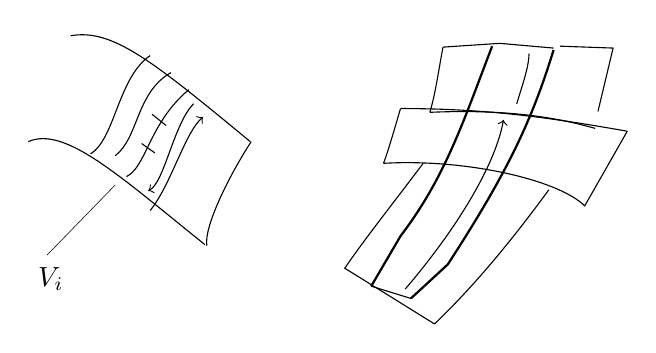
\begin{tikzpicture}[x=0.12mm,y=-0.12mm]
\draw (63,18) .. controls (107,10) and (150,45) .. (253,130);
\draw (18,130) .. controls (57,113) and (115,167) .. (205,239);
\draw (254,130) .. controls (230,167) and (204,220) .. (207,240);
\draw (84,143) .. controls (110,127) and (113,62) .. (147,39);
\draw (110,145) .. controls (135,126) and (132,78) .. (169,57);
\draw (122,167) .. controls (143,157) and (146,110) .. (188,75);
\draw (138,132)--(152,142);
\draw (149,101)--(164,113);
\draw[->] (193,90) .. controls (172,111) and (162,174) .. (145,182);
\draw[->] (147,203) .. controls (169,176) and (184,120) .. (203,104);
\draw[line width=0.2pt] (38,250)--(110,176);
\node[below] at (42,253) {$V_i$};
\begin{scope}[xshift=40.44mm]
\draw (120,30)--(180,26)--(237,31);
\draw (244,29)--(300,31)--(284,98);
\draw (106,99) .. controls (112,80) and (116,50) .. (120,30);
\draw (106,99) .. controls (197,95) and (249,107) .. (281,116);
\draw (75,95) .. controls (70,112) and (62,140) .. (57,153);
\draw (75,95) .. controls (169,95) and (235,105) .. (315,119);
\draw (57,153) .. controls (140,148) and (240,169) .. (270,198)--(315,119);
\draw[line width=0.8pt] (172,29) .. controls (142,107) and (123,167) .. (75,230)--(44,283);
\draw[line width=0.8pt] (237,33) .. controls (214,108) and (188,163) .. (125,260)--(86,296);
\draw (99,153) .. controls (65,198) and (35,236) .. (16,264)--(111,323);
\draw (111,323) .. controls (158,278) and (199,226) .. (232,181);
\draw (44,283)--(86,296);
\draw[->] (80,286) .. controls (124,235) and (174,162) .. (184,107);
\draw (198,90) .. controls (203,73) and (211,51) .. (211,37);
\end{scope}
\end{tikzpicture}
}}
\end{GelfandAdjacentEvidence}
\begin{GelfandAdjacentEvidence}{GELFAND-P000227}{6}

\begin{equation*}
 \lambda_i h^{-1}=\sum\lambda_i'=\sum\pi_{ii'}\lambda_{i'},\quad\text{т. е.}
\end{equation*}
\Unclear{GELFAND-P000227}{first-sum-prime}{В первой сумме штрих расположен высоко: $\sum\lambda_i'$ / $\sum\lambda_{i'}$; отображён первый кандидат.}
\end{GelfandAdjacentEvidence}

\begin{equation*}
 \fbox{$h^{-1}\vec\lambda=\Pi\vec\lambda$.}
\end{equation*}
— собств. вектор.



\begin{GelfandAdjacentEvidence}{GELFAND-P000227}{7}
(Это при наших
\Unclear{GELFAND-P000227}{bottom-cancelled-word}{Зачёркнутая короткая запись неразборчива.}


пар-мах).



На отрезке знач. меры есть. Далее из 2-го св-ва.

[Под последней строкой:] (на отр. поменьше)
\end{GelfandAdjacentEvidence}







\begin{GelfandAdjacentEvidence}{GELFAND-P000228}{1}
\SourcePage{GELFAND-P000228}{unlabelled}
\Unclear{GELFAND-P000228}{title-ending}{Энтропия / Энтропии; окончание не установлено однозначно.}


\begin{equation*}
 T=\left|\begin{array}{ccc}a&\cdot&b\\c&&d\end{array}\right|
\end{equation*}



\begin{equation*}
 h(T)=\ln\lambda\quad(\lambda>1)
\end{equation*}



\begin{equation*}
 h(T)=\lambda
\end{equation*}
\end{GelfandAdjacentEvidence}



$\Rightarrow$ преобр. метрически изоморфны.

\begin{GelfandAdjacentEvidence}{GELFAND-P000228}{2}
$\Omega_{\Pi_1}$ отобр. на $\Omega_{\Pi_0}$ (станд.) —



\Unclear{GELFAND-P000228}{earlier-abbreviation}{прежн. раз. / прим. раз.; первое сокращение не установлено.}
\end{GelfandAdjacentEvidence}


И осталось тор. отобр. на $\Omega_{\Pi_1}$.

\begin{GelfandAdjacentEvidence}{GELFAND-P000228}{3}
$\Pi_1$ определённого типа: 4 группы букв и св-ва
перех. — см. ранее.







\Unclear{GELFAND-P000228}{torus-partition}{Почти прямоугольная рамка, наклонные рёбра с выступами сверху, справа и снизу и штриховка. В густых пересечениях продолжения линий и точные границы заштрихованных частей не установлены однозначно. Подписей вершин и стрелок нет.\par\smallskip\centering{\color{black}\GelfandFitDiagram{
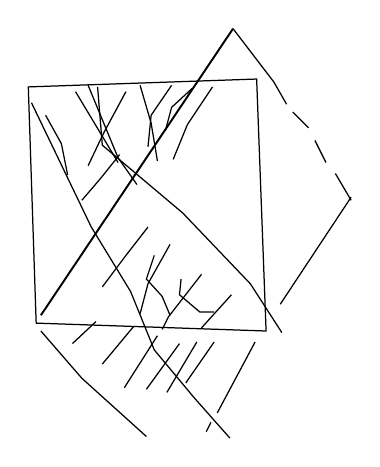
\begin{tikzpicture}[x=0.20mm,y=-0.20mm,line width=0.45pt]
\draw (30,55)--(175,50)--(181,210)--(35,205)--cycle;
\draw[line width=0.7pt] (38,200)--(160,18);
\draw (32,65)--(70,144)--(95,185)--(110,222)--(135,252)--(158,278);
\draw (74,55)--(77,92)--(128,135)--(171,180)--(191,211);
\draw (160,18)--(186,52)--(194,66);
\draw (198,71)--(208,81);
\draw (212,89)--(219,103);
\draw (225,110)--(235,127);
\draw (235,125)--(190,193);
\draw (38,210)--(64,240)--(105,277);
\draw (150,262)--(174,217);
\draw (146,268)--(143,274);
\draw (60,58)--(72,78)--(87,103);
\draw (41,73)--(51,91)--(55,111);
\draw (68,54)--(87,100)--(99,117);
\draw (101,54)--(108,78)--(112,102);
\draw (121,54)--(108,73)--(106,93);
\draw (92,58)--(78,84)--(68,105);
\draw (147,55)--(131,79)--(122,101);
\draw (134,56)--(121,68)--(117,83);
\draw (88,98)--(76,113)--(64,127);
\draw (106,144)--(92,162)--(77,182);
\draw (120,155)--(106,180)--(101,199);
\draw (140,174)--(119,201)--(115,209);
\draw (159,187)--(140,208);
\draw (110,162)--(105,177)--(115,188)--(120,200);
\draw (127,177)--(126,187)--(139,198)--(148,198);
\draw (58,218)--(73,204);
\draw (77,231)--(97,207);
\draw (91,246)--(112,213);
\draw (105,247)--(126,218);
\draw (118,249)--(137,217);
\draw (130,243)--(148,217);
\end{tikzpicture}
}}\par\smallskip}
\end{GelfandAdjacentEvidence}

— разб. тора на 2 параллелограмма
(стороны $\parallel$ соб. напр.)



\begin{GelfandAdjacentEvidence}{GELFAND-P000228}{4}

Стороны леж. на прямой, прох. через 0
по собств. напр. (и \Unclear{GELFAND-P000228}{parenthetical-direction}{продолж. / проек.; средние штрихи сокращения слиты.}

).
\end{GelfandAdjacentEvidence}

Это Марковское разбиение (самое крупное).
Из-за него и удаётся решить пробл. изоморфизма.



\begin{GelfandAdjacentEvidence}{GELFAND-P000228}{5}

\begin{equation*}
 \bigcap T^n V_{\omega_n}
\end{equation*}
\Unclear{GELFAND-P000228}{intersection-subscript}{Под $V$ запись $\omega_n$ / $\omega$; отдельный нижний $n$ не установлен. У знака пересечения отдельного индекса не видно.}


может сост. из больш. числа точек.
\end{GelfandAdjacentEvidence}

\begin{GelfandAdjacentEvidence}{GELFAND-P000228}{6}
Рассм. сначала 4 пар-на:
\begin{gather*}
 V_1\cap TV_1\\
 V_2\cap TV_2\\
 V_1\cap TV_2\\
 V_1\cap TV_2
\end{gather*}



\Unclear{GELFAND-P000228}{second-pair}{Второе пересечение: $V_2\cap TV_2$ / $V_2\cap TV_1$. Правый индекс густо обведён; отображён первый кандидат.}
\end{GelfandAdjacentEvidence}




\begin{GelfandAdjacentEvidence}{GELFAND-P000228}{7}

(\Unclear{GELFAND-P000228}{uzhe-cancellation}{Уже; слово читается, наличие зачёркивания поперечным штрихом не установлено.}
 несвязн. разбиение. Образ. разбиение —
— его связные комп. Их числа соотв. —
— \Unclear{GELFAND-P000228}{component-counts}{$p,q,r,s$; второй знак густо обведён, чтение $q$ остаётся кандидатом.}

)
\end{GelfandAdjacentEvidence}





\begin{GelfandAdjacentEvidence}{GELFAND-P000229}{91}
\SourcePage{GELFAND-P000229}{unlabelled}
\underline{\underline{1968 год.}}

12/\underline{II}\quad\underline{Вопрос} (Гельфанд)



$R$ — счётнонорм. кольцо:




\begin{equation*}
 \lVert xy\rVert_i\leq\lVert x\rVert_k\lVert y\rVert_\ell
\end{equation*}
\Unclear{GELFAND-P000229}{norm-final-index}{Последний индекс: $\ell$ / $e$; отображён $\ell$.}

\end{GelfandAdjacentEvidence}
\begin{GelfandAdjacentEvidence}{GELFAND-P000229}{2}





\SourceFigure{GELFAND-P000229}{stepped-theorem-frame}{\par\smallskip\centering{\color{black}\GelfandFitDiagram{
\begin{tikzpicture}[x=1mm,y=1mm]
\draw (0,0)--(0,13)--(16,17)--(16,27)--(51,25)--(51,16)--(76,13)--(76,1)
 .. controls (72,1) and (70,4) .. (66,2)
 .. controls (62,-1) and (58,-1) .. (54,2)
 .. controls (50,4) and (46,4) .. (42,1)
 .. controls (38,-2) and (34,-2) .. (30,1)
 .. controls (26,4) and (22,4) .. (18,1)
 .. controls (14,-2) and (10,-2) .. (6,1)--(0,0);
\node at (33,20) {\underline{Теор.}};
\node at (38,6) {Гельфанд–Наймарк};
\end{tikzpicture}
}}\par\smallskip}
\end{GelfandAdjacentEvidence}
\begin{GelfandAdjacentEvidence}{GELFAND-P000229}{92}


для \Unclear{GELFAND-P000229}{superscribed-mark}{[Надстрочный знак: наложенные петли и штрихи; чтение не установлено.]}



норм. кольц:
\begin{equation*}
 f(x^*x)\geq0\Rightarrow f(x)=\int_{\mathcal M_0}x(M)\,d\sigma(M)
\end{equation*}
($\mathcal M_0$ — симм. ид.)
\Unclear{GELFAND-P000229}{ideal-space-notation}{В нижнем пределе и в пояснении буква $M_0$ / $m_0$ / $\mathcal M_0$; нижний нуль читается. Регистр и стиль буквы не установлены; отображён $\mathcal M_0$.}

\end{GelfandAdjacentEvidence}

Перенос — ? (Не всегда: надо
охар. аксиом. класс).



\begin{equation*}
 x^*(M)=\overline{x(M')},\quad M=M'
\end{equation*}
— симм.



$L^1$ со свёрткой, $\overline{x(-t)}=x^*(t)$



$\Rightarrow$ теор. Бохнера
\begin{equation*}
 \int_{-\infty}^{+\infty}e^{it\lambda}\,d\sigma(t)
\end{equation*}



\begin{GelfandAdjacentEvidence}{GELFAND-P000229}{5}
\underline{\underline{И. Бернштейн.}}




\SourceFigure{GELFAND-P000229}{topology-heading}{\par\smallskip\centering{\color{black}\GelfandFitDiagram{
\begin{tikzpicture}[x=1mm,y=1mm]
\node[anchor=base] at (69,0) {Топология Гротендика.};
\draw (0,-2) .. controls (2,-1) and (4,-1) .. (6,-2)
 .. controls (8,-3) and (10,-3) .. (12,-2)
 .. controls (14,-1) and (16,-1) .. (18,-2)
 .. controls (20,-3) and (22,-3) .. (24,-2)
 .. controls (26,-1) and (28,-1) .. (30,-2)
 .. controls (32,-3) and (34,-3) .. (36,-2)
 .. controls (38,-1) and (40,-1) .. (42,-2)
 .. controls (44,-3) and (46,-3) .. (48,-2)
 .. controls (50,-1) and (52,-1) .. (54,-2)
 .. controls (56,-3) and (58,-3) .. (60,-2)
 .. controls (62,-1) and (64,-1) .. (66,-2)
 .. controls (68,-3) and (70,-3) .. (72,-2)
 .. controls (74,-1) and (76,-1) .. (78,-2)
 .. controls (80,-3) and (82,-3) .. (84,-2)
 .. controls (86,-1) and (88,-1) .. (90,-2)
 .. controls (92,-3) and (94,-3) .. (96,-2)
 .. controls (98,-1) and (100,-1) .. (102,-2)
 .. controls (104,-3) and (106,-3) .. (108,-2)
 .. controls (110,-1) and (112,-1) .. (114,-2)
 .. controls (116,-3) and (118,-3) .. (120,-2)
 .. controls (122,-1) and (124,-1) .. (126,-2)
 .. controls (128,-3) and (130,-3) .. (132,-2)
 .. controls (134,-1) and (136,-1) .. (138,-2);
\end{tikzpicture}
}}\par\smallskip}
\end{GelfandAdjacentEvidence}

$T$ — это след. совокупность:

1) Категория $\operatorname{Cat}T$ выделена (объекты — откр. мн-ва).

2) Выделены нек-рые сем-ва $\{\alpha_i:U_i\to U\}$,
называемые покрытиями

\begin{GelfandAdjacentEvidence}{GELFAND-P000229}{93}
3) Выд. система, уд. аксиомам:




1. Сущ. пересечение — \underline{произведение} (расслоенное).




\SourceFigure{GELFAND-P000229}{fiber-product-diagram}{\par\smallskip\centering{\color{black}\GelfandFitDiagram{
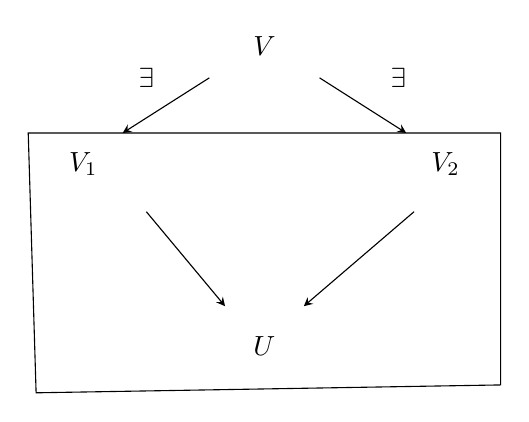
\begin{tikzpicture}[x=1mm,y=1mm,>=stealth]
\node at (30,38) {$V$};
\node at (7,23) {$V_1$};
\node at (53,23) {$V_2$};
\node at (30,0) {$U$};
\draw[->] (23,34)--(12,27);
\draw[->] (37,34)--(48,27);
\node at (15,34) {$\exists$};
\node at (47,34) {$\exists$};
\draw[->] (15,17)--(25,5);
\draw[->] (49,17)--(35,5);
\draw (0,27)--(60,27)--(60,-5)--(1,-6)--cycle;
\end{tikzpicture}
}}\par\smallskip}



(коммут.).




\SourceFigure{GELFAND-P000229}{given-data-caption}{\par\smallskip\centering{\color{black}\GelfandFitDiagram{
\begin{tikzpicture}[x=1mm,y=1mm]
\node[anchor=west] at (0,10) {— \underline{дано 3 об.}};
\node[anchor=west] at (16,0) {\underline{и 2 отобр.}};
\draw (17,-3)--(62,-3)--(62,15);
\draw (64,-2)--(64,15);
\end{tikzpicture}
}}\par\smallskip}

\end{GelfandAdjacentEvidence}
\begin{GelfandAdjacentEvidence}{GELFAND-P000229}{8}

\fbox{$V=V_1\times_U V_2$} — обозначение.
Тогда сущ.







\SourceFigure{GELFAND-P000229}{open-set-sketch}{\par\smallskip\centering{\color{black}\GelfandFitDiagram{
\begin{tikzpicture}[x=1mm,y=1mm]
\draw (15,15) .. controls (-11,4) and (-22,-17) .. (2,-29)
 .. controls (23,-39) and (49,-18) .. (49,3)
 .. controls (49,17) and (36,23) .. (24,18);
\draw[rotate=32] (6,-5) ellipse (9mm and 5mm);
\draw[rotate=32] (15,-3) ellipse (9mm and 7mm);
\draw (12,-6)--(15,2);
\node at (65,-4) {$U$};
\end{tikzpicture}
}}\par\smallskip}
\end{GelfandAdjacentEvidence}

\begin{GelfandAdjacentEvidence}{GELFAND-P000229}{9}
Треб. вып. универс. св-ва:

$\forall X$, и $\forall$







\Unclear{GELFAND-P000229}{universal-diagram}{Четыре наружные стрелки: $X\to V_1$, $X\to V_2$, $V\to V_1$, $V\to V_2$. На обоих концах густого центрального соединения видны клиновидные штрихи; направленность и наличие исправления не установлены. Видимые наконечники сохранены, но однозначное универсальное отображение ими не установлено. Выносная линия ведёт к «сущ. и единств.».\par\smallskip\centering{\color{black}\GelfandFitDiagram{
\begin{tikzpicture}[x=1mm,y=1mm,>=stealth]
\node at (0,4) {$X$};
\node at (32,17) {$V_1$};
\node at (31,-13) {$V_2$};
\node at (68,0) {$V$};
\draw[->] (8,8)--(26,15);
\draw[->] (7,-3)--(25,-12);
\draw[->] (61,7)--(40,16);
\draw[->] (62,-8)--(42,-16);
\draw[line width=0.9pt] (12,1)--(60,-3);
\draw[line width=0.8pt] (20,5)--(12,1)--(20,-3);
\draw[line width=0.8pt] (53,1)--(60,-3)--(53,-7);
\draw (48,-7) .. controls (56,-9) and (57,-19) .. (65,-26);
\node[anchor=west] at (65,-26) {сущ. и единств.};
\end{tikzpicture}
}}\par\smallskip}
\end{GelfandAdjacentEvidence}

От $U$ существенно зависит (в топ. Гротенд.)

(Если $V$ сущ., то он опред. однозн. по св-вам категории)





\begin{GelfandAdjacentEvidence}{GELFAND-P000230}{1}
\SourcePage{GELFAND-P000230}{unlabelled}




\Unclear{GELFAND-P000230}{upper-right-label}{В правом верхнем углу $18$ / $98$; первая цифра утолщена. Отображён кандидат $18$ и угловая рамка.\par\smallskip\centering{\color{black}\GelfandFitDiagram{
\begin{tikzpicture}[x=1mm,y=1mm]
\draw (0,20)--(0,0)--(24,1);
\node at (13,10) {$18$};
\end{tikzpicture}
}}\par\smallskip}
\end{GelfandAdjacentEvidence}

2. $\{U\overset{\mathrm{id}}{\longrightarrow}U\}$ — покрытие.



3. $\{V_i\to V\}$ — покр.

$\{V_{ij}\to V_i\}$ — покр.

$\Rightarrow\{V_{ij}\to V\}$ — покр.



4. $\{U_i\to U\}$ — покрытие

$\{V\to U\}$ — морфизм

Тогда $\{U_i\times_U V\to V\}$



\underline{Пример:} неразветвл. топология.

$X$ — обычн. топ. пр-во.



Откр. мн-во: $U\to X$ — лок. гомеоморфизм

($U$ — топ. пр.)



\begin{GelfandAdjacentEvidence}{GELFAND-P000230}{2}
(накрытие над $X$ или его откр. \Unclear{GELFAND-P000230}{open-subset-word}{подмн-вом / мн-вом с возможной отменой начального «под»; отдельное зачёркивание не установлено.}

).
\end{GelfandAdjacentEvidence}

\begin{GelfandAdjacentEvidence}{GELFAND-P000230}{3}
Отображение




\SourceFigure{GELFAND-P000230}{morphism-triangle}{\par\smallskip\centering{\color{black}\GelfandFitDiagram{
\begin{tikzpicture}[x=1mm,y=1mm,>=stealth]
\node at (0,20) {$U$};
\node at (0,-9) {$V$};
\node at (42,20) {$X$};
\draw[->] (8,20)--(34,20);
\draw[->] (0,-2)--(0,12);
\draw[->] (11,-1)--(34,12);
\end{tikzpicture}
}}\par\smallskip}
\end{GelfandAdjacentEvidence}

(любое непр. с комм. диагр.)



\begin{GelfandAdjacentEvidence}{GELFAND-P000230}{4}
$\{U_i\to U\}$ — покр., если образы
\Incomplete{GELFAND-P000230}{crossed-word}{[Зачёркнутое слово не разобрано.]}


покрывают.
\end{GelfandAdjacentEvidence}



\begin{GelfandAdjacentEvidence}{GELFAND-P000230}{5}
\underline{Аксиома 1.}







\SourceFigure{GELFAND-P000230}{circle-sketch}{\par\smallskip\centering{\color{black}\GelfandFitDiagram{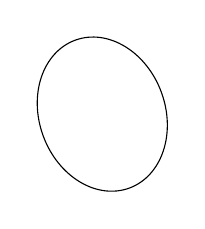
\begin{tikzpicture}[x=1mm,y=1mm]
\draw[rotate=20] (0,0) ellipse (8mm and 10mm);
\end{tikzpicture}}}\par\smallskip}
\end{GelfandAdjacentEvidence}

$U$ — окр., $U$ — тоже окр., отобр. со степ. 2
$U\to U$.



\begin{GelfandAdjacentEvidence}{GELFAND-P000230}{6}
\begin{equation*}
 U\times_U U=U.
\end{equation*}







\SourceFigure{GELFAND-P000230}{degree-two-diamond}{\par\smallskip\centering{\color{black}\GelfandFitDiagram{
\begin{tikzpicture}[x=1mm,y=1mm,>=stealth]
\node at (20,30) {$U$};
\node at (0,13) {$U$};
\node at (40,13) {$U$};
\node at (20,-6) {$U$};
\draw[->] (14,26)--(5,18);
\draw[->] (26,26)--(35,18);
\draw[->] (5,7)--(14,-1);
\draw[->] (35,7)--(26,-1);
\end{tikzpicture}
}}\par\smallskip}
\end{GelfandAdjacentEvidence}
\begin{GelfandAdjacentEvidence}{GELFAND-P000230}{7}

$U_1\times_X U_2$ —
\Unclear{GELFAND-P000230}{join-operations}{перемн. и склеив. / пересеч. и склеив.; первое сокращение не установлено однозначно.}
\end{GelfandAdjacentEvidence}

— несвязное объед.

2 и 3 листа $\Rightarrow$ 6 листов



\begin{gather*}
 \mathbb Z_2\times\mathbb Z_2\ne\mathbb Z_4,\\
 \mathbb Z_2\times\mathbb Z_3=\mathbb Z_6.
\end{gather*}





\SourcePage{GELFAND-P000231}{unlabelled}
Предпучок: $\bullet$ функтор



\begin{gather*}
 \operatorname{Cat}T\to\mathrm{Ab}\qquad\text{(контравар.)}\\
 u\to P(u)
\end{gather*}



\begin{equation*}
 v\to u\;\Rightarrow\;P(u)\to P(v)
\end{equation*}



\begin{GelfandAdjacentEvidence}{GELFAND-P000231}{0}
Пучок — предпучок, удовл. аксиомам:



1. $\xi\in P(u)$

$\{u_i\to u\}$ — покрытие
\begin{equation*}
 \xi\to\xi_i\qquad P(u)\to P(u_i)
\end{equation*}
$\xi$ — однозн. опр. $\xi_i$




\end{GelfandAdjacentEvidence}
\begin{GelfandAdjacentEvidence}{GELFAND-P000231}{1}
2. и действ. опр., если $\xi_i$ совп. на пересеч.







\SourceFigure{GELFAND-P000231}{framed-intersection}{\par\smallskip\centering{\color{black}\GelfandFitDiagram{
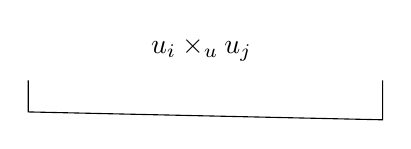
\begin{tikzpicture}[x=1mm,y=1mm]
\node at (22,5) {$u_i\times_u u_j$};
\draw (0,1)--(0,-3)--(45,-4)--(45,1);
\end{tikzpicture}
}}\par\smallskip}
\end{GelfandAdjacentEvidence}

Когомологии Чеха определим



\begin{align*}
 C^0&=P(u)\\
 C^1&=\prod P(u_i)\\
 C^2&=\prod P(u_i\times_u u_j).\\
 C^3&=\prod P(u_i\times_u u_j\times_u u_k)
\end{align*}



$d$ опред. естеств



$\mathcal F\to\Gamma(X,\mathcal F)$ — функтор.



\begin{GelfandAdjacentEvidence}{GELFAND-P000231}{2}
\begin{center}
\begin{tabular}{l}
($\Gamma$ — аб. группа —\\
\hspace{12mm}— пучок групп)
\end{tabular}
\end{center}
\Unclear{GELFAND-P000231}{gamma-gloss}{Обе строки скобки сохранены. Перед тире второй строки отдельного обозначения не видно; подразумеваемое подлежащее не установлено.}
\end{GelfandAdjacentEvidence}

\begin{equation*}
 0\to\mathcal F_1\to\mathcal F_2\to\mathcal F_3\to0.
\end{equation*}



— \underline{точн. посл. пучков.}



\begin{equation*}
 0\to\Gamma(\mathcal F_1)\to\Gamma(\mathcal F_2)\to\Gamma(\mathcal F_3)
\end{equation*}



(точный слева).



\begin{GelfandAdjacentEvidence}{GELFAND-P000231}{91}
Сущ. производные функторы. $R^i:S\to\mathrm{Ab}$



$S$ — произв. пучки (категория).



\begin{equation*}
 \to R^1(\mathcal F_1)\to\ldots\to R^2(\mathcal F_2)
\end{equation*}



($R^i$ — опр. однозначно).
\begin{equation*}
 R^i(\mathcal F)\underset{\mathrm{def}}{=}H^i(X,\mathcal F).
\end{equation*}




\end{GelfandAdjacentEvidence}\begin{GelfandAdjacentEvidence}{GELFAND-P000231}{3}
\underline{Кон. группа.} Топ. Гротендика из представлений.







\SourceFigure{GELFAND-P000231}{source-icon}{Отдельный значок на исходном изображении.\par\smallskip\centering{\color{black}\GelfandFitDiagram{

\begin{tikzpicture}[x=1mm,y=1mm,line width=0.6pt]
\path[draw=black,fill=yellow] (3,3)--(8,3)--(7,0)--(11,3)--(22,3)
 .. controls (25,3) and (26,5) .. (26,8)--(26,17)
 .. controls (26,20) and (24,22) .. (21,22)--(4,22)
 .. controls (1,22) and (0,20) .. (0,17)--(0,8)
 .. controls (0,5) and (1,3) .. (3,3)--cycle;
\draw (5,17)--(21,17);
\draw (5,12)--(21,12);
\draw (5,7)--(17,7);
\end{tikzpicture}
}}\par\smallskip}
\end{GelfandAdjacentEvidence}



\SourcePage{GELFAND-P000232}{unlabelled}
11/III \underline{Гельфанд} (и Кириллов)



$\mathfrak g$ — полупростая алгебра Ли, (над $C$)



$U(\mathfrak g)$ — её обёрт. алгебра



(полин. от обр. $e_1,\ldots,e_n$,
\begin{equation*}
 e_i e_k-e_k e_i=\sum C^j_{ik}e_j
\end{equation*}



$Z(\mathfrak g)$ — центр обёрт. алгебры

(её элем. — опер. Лапласа или Казимира).



Предст. $G\Rightarrow$ дифф. опер. и коммут.



\begin{GelfandAdjacentEvidence}{GELFAND-P000232}{1}
$Z(\mathfrak g)$ — коммут. с действ. \Unclear{GELFAND-P000232}{centre-end}{групп}
\end{GelfandAdjacentEvidence}


Такое предст. обёрт. алг. дифф. операторами не обяз. точное.



На самой $G$ — точное (преобр.)



Для $Z(\mathfrak g)$ всё равно левые или правые.



$\mathfrak g$ — полупростая алгебра Ли. (над $C$).



\begin{GelfandAdjacentEvidence}{GELFAND-P000232}{2}
$N_-$ — $\max$ нильпот. \Unclear{GELFAND-P000232}{nilpotent-corrections}{[зачёркнуто: группа алгебра] [ниже первого слова вписано: группа]}
\end{GelfandAdjacentEvidence}
\begin{GelfandAdjacentEvidence}{GELFAND-P000232}{3}
 (треуг. матр.)

\Unclear{GELFAND-P000232}{quotient-correction}{$N_-\backslash G$ [верхний правый знак густо обведён]}
\end{GelfandAdjacentEvidence}


\begin{GelfandAdjacentEvidence}{GELFAND-P000232}{4}
\underline{Теорема:} в $N_-\backslash G$ предст. $U(\mathfrak g)$ точно.



\Unclear{GELFAND-P000232}{theorem-adjective}{(простой).}
\end{GelfandAdjacentEvidence}


$f$ на группе регулярна, если сдвиги — конечномерн. пр-во

($\sin$ на прямой)



На комп. группе ф-и аппрокс. регулярными (теор. о полноте)



Рассм. ф-и $f(g)\equiv f(n_-g)$ — инвар. — кольцо.



Рассм. $\operatorname{Spec}$ этого кольца. Это $X$.



$N_-\backslash G$ бирац. эквив. проект. пр-ву.



Обёрт. алгебр много, но тел, частных немного



\begin{equation*}
 \underset{\substack{\text{тело}\\\text{отнош.}}}{D(\mathfrak g)}\sim D_{n,k}
\end{equation*}



Нетрив., что вклад. в тело (!) отнош.



\begin{GelfandAdjacentEvidence}{GELFAND-P000232}{5}
\begin{equation*}
 x_1,\ldots,x_n;\quad
 \frac{\partial}{\partial x_1},\ldots,\frac{\partial}{\partial x_n},\quad
 y_1,\ldots,y_k
\end{equation*}



\Unclear{GELFAND-P000232}{operator-letter}{$\ell(x,\frac{\partial}{\partial x},y)$}
\end{GelfandAdjacentEvidence}


$\underline{\underline{QP^{-1}}}\;Q_1P_1^{-1}$ и т.д. всё можно в 2 шага.

(дост. $QP^{-1}$)



$n$ — число перем., $k$ — число парам. — инварианты.





\begin{GelfandAdjacentEvidence}{GELFAND-P000233}{1}
\SourcePage{GELFAND-P000233}{23}




\SourceFigure{GELFAND-P000233}{source-number}{\par\smallskip\centering{\color{black}\GelfandFitDiagram{
\begin{tikzpicture}[x=1mm,y=1mm]
\node at (9,6) {$23$};
\draw (0,14)--(0,0)--(18,0);
\end{tikzpicture}
}}\par\smallskip}
\end{GelfandAdjacentEvidence}\begin{GelfandAdjacentEvidence}{GELFAND-P000233}{91}


Для полупр. группы почти док., что $D(\mathfrak g)\sim D_{n,k}$.




(\Unclear{GELFAND-P000233}{top-parenthesis}{постр.}

 верна)

\end{GelfandAdjacentEvidence}

\begin{GelfandAdjacentEvidence}{GELFAND-P000233}{3}
Для нильп. док. и вероятно для алгебр. разрешимых.




\SourceFigure{GELFAND-P000233}{central-extension}{\par\smallskip\centering{\color{black}\GelfandFitDiagram{\begin{minipage}{68mm}\raggedright 
Присоед. к $Z(\mathfrak g)$ \tikz[baseline=(k.base)]{\node[draw,circle,inner sep=1pt] (k) {$K$};} операторов — виртуальные опер. Лапласа
\end{minipage}}}\par\smallskip}
\end{GelfandAdjacentEvidence}
\begin{GelfandAdjacentEvidence}{GELFAND-P000233}{4}

Новое кольцо $\tilde U(\mathfrak g)$ — с присоед. левыми сдвигами



\Incomplete{GELFAND-P000233}{crossed-top}{Зачёркнуто короткое слово или сокращение; буквенное чтение под густыми штрихами не установлено.}
\end{GelfandAdjacentEvidence}

\begin{equation*}
 U(\mathfrak g)\otimes_{Z(\mathfrak g)}\tilde Z(\mathfrak g)=\tilde U(\mathfrak g).
\end{equation*}



$\tilde Z$ — $Z$ с при-соед. вирт. опер. Лапл.



(это алгебр. расшир., гр. Галуа — гр. Вейля).



\underline{Теорема.} Тело частных $\tilde U(\mathfrak g)$ есть $D_{n,k}$.



(Для $U$ неизв.; сделано для унимодулярных).



Алг. расшир. $D_{n,k}$ — ?.



\begin{GelfandAdjacentEvidence}{GELFAND-P000233}{5}
В коммут. случае алг. мн-зия.




\SourceFigure{GELFAND-P000233}{question}{\par\smallskip\centering{\color{black}\GelfandFitDiagram{\begin{minipage}{68mm}\raggedright 
\underline{Вопрос.} Есть компактные \begin{tikzpicture}[x=1mm,y=1mm,baseline=(c.base)]
\node[inner sep=1pt] (c) at (15,5) {компл.};
\draw (1,8).. controls (6,12) and (28,12) .. (31,8)
 .. controls (36,2) and (28,1) .. (16,1)
 .. controls (9,2) and (7,0) .. (5,-4)
 --(5,0).. controls (-1,0) and (-3,4) .. (1,8);
\end{tikzpicture} мн-зие.

Описать регулярные дифф. операторы
\end{minipage}}}\par\smallskip}
\end{GelfandAdjacentEvidence}

На сф. Римана $\frac{\partial}{\partial z},\;z\frac{\partial}{\partial z},\;z^2\frac{\partial}{\partial z}$



\underline{О раб. Диксмье} (Лиманов).



\begin{GelfandAdjacentEvidence}{GELFAND-P000233}{6}
$R_{1,0}$ — кольцо квант. мех. — обр. $x,\frac{d}{dx}$.







\SourceFigure{GELFAND-P000233}{polynomial-callout}{\par\smallskip\centering{\color{black}\GelfandFitDiagram{
\begin{tikzpicture}[x=1mm,y=1mm]
\node[anchor=west] at (5,15) {Полиномы};
\node[anchor=west] at (5,5) {от $p$ и $q$.};
\draw (0,0)--(1,21);
\draw (2,0)--(3,21);
\draw (5,-2)--(56,-3);
\end{tikzpicture}
}}\par\smallskip}
\end{GelfandAdjacentEvidence}

$p,q,\quad [p,q]=1$.



\begin{GelfandAdjacentEvidence}{GELFAND-P000233}{7}
Группа автом. порождается треуг. автом.



\Unclear{GELFAND-P000233}{first-shear}{$\left\{\begin{aligned}p&\to p\\q&\to q+f(p)\end{aligned}\right.$}
\end{GelfandAdjacentEvidence}

и
$\left\{\begin{aligned}p&\to p+g(q)\\q&\to q\end{aligned}\right.$



Для тела $D_{1,0}$ неизвестно.



\begin{GelfandAdjacentEvidence}{GELFAND-P000233}{8}
Или \Unclear{GELFAND-P000233}{bottom-cancellation}{[зачёркнутый знак: и? от?]}
\end{GelfandAdjacentEvidence}


$\left\{\begin{aligned}q&\to q\\p&\to p+g(q)\end{aligned}\right.$



и
$\left\{\begin{aligned}q&\to p\\p&\to -q\end{aligned}\right.$

(преобр. Фурье)



Порождается





\SourcePage{GELFAND-P000234}{unlabelled}
Арнольд: теор.



\begin{GelfandAdjacentEvidence}{GELFAND-P000234}{1}
Пусть есть ф-и $f(p,q)$



\Unclear{GELFAND-P000234}{poisson-index}{$[f_1(p,q),f_2(p,q)]=\dfrac{\partial f_1}{\partial p}\cdot\dfrac{\partial f_2}{\partial q}-\dfrac{\partial f_1}{\partial q}\cdot\dfrac{\partial f_2}{\partial p}$. [Индекс в первом множителе после минуса: $1$ или $2$.]}
\end{GelfandAdjacentEvidence}

Рассм. 2 полинома
\begin{gather*}
 P=P(p,q)\\
 Q=Q(p,q).
\end{gather*}



Подст. $P$ и $Q$ — будет 1.



Они индуц. канонич. преобр. квазиклассики.



Но связи нет, даже с градуировкой.



Элемент $x$ вполне полупростой, если преобр. $\operatorname{ad}X$ имеет полн. сист. собств. значений.



\begin{GelfandAdjacentEvidence}{GELFAND-P000234}{2}
Тогда автоморф. $x$ переводится в $x\to pq$.




\SourceFigure{GELFAND-P000234}{euler}{\par\smallskip\centering{\color{black}\GelfandFitDiagram{\begin{minipage}{68mm}\raggedright 
\begin{tikzpicture}[x=1mm,y=1mm,baseline=(e.base)]
\node[inner sep=0pt] (e) at (11,7) {$x\dfrac{d}{dx}$};
\draw (-2,3)--(-2,0)--(24,0)--(24,3);
\end{tikzpicture} — соб. ф-и — однор. многочлены.
\end{minipage}}}\par\smallskip}
\end{GelfandAdjacentEvidence}

\begin{equation*}
 p^a q^b\to(a-b)p^a q^b.
\end{equation*}



\begin{GelfandAdjacentEvidence}{GELFAND-P000234}{3}
Рез. \Unclear{GELFAND-P000234}{amitsur-name}{Амицури или Амицура}

:

$x$\qquad $C(x)$ — коммутирующие — коммут. подалгебра.
\end{GelfandAdjacentEvidence}



Но это не всегда многочлены.



\begin{equation*}
 \forall\alpha\ \exists X,Y,\qquad X^3=Y^2+\alpha,\qquad \alpha\in C.
\end{equation*}



\underline{Паламодов.}



о раб. Хёрмандера (по $\bar\partial$)



2 осн. рез.: теор. сущ. и теор. аппрокс.



1. $\Omega\subset C^n$, $\phi\in C^2(\Omega)$
\begin{equation*}
 L(\phi)=\frac{\partial^2\phi}{\partial z_j\partial\bar z_k}\xi_j\bar\xi_k\ge0
\end{equation*}



\begin{equation*}
 L_{p,q}=L_{p,q}(\Omega,\phi),\qquad
 \|f\|_\phi^2=\int_\Omega |f|^2e^{-\phi}dV
\end{equation*}
формы типа $(p,q)$



\begin{GelfandAdjacentEvidence}{GELFAND-P000234}{4}
Пусть $\phi$ — плюрисубг. в $\Omega$ \Unclear{GELFAND-P000234}{plurisub-correction}{[наложенные штрихи перед скобкой]}
\end{GelfandAdjacentEvidence}
 (стало быть вещ.) и

$\forall c\ \{\phi\le c\}$ — компакт. ($\Rightarrow\Omega$ — псевдовыпукла)



Тогда $\forall f\in L_{p,q}$, $\bar\partial f=0$



\begin{GelfandAdjacentEvidence}{GELFAND-P000234}{5}
$\exists$ \Incomplete{GELFAND-P000234}{cancelled-existence}{Зачёркнутый фрагмент; начальный знак похож на $g$, остальное буквенное чтение не установлено.}
\end{GelfandAdjacentEvidence}

$g$ типа $p,q-1$



\begin{equation*}
 \bar\partial g=f\qquad\overset{(q\ge1)}{\text{и}}\qquad
 g\in L_{p,q-1}(\Omega,\phi+2\ln(1+|z|^2))
\end{equation*}



При этом $\sqrt q\,\|g\|\le\|f\|$ (предполаг. $q\ge1$)





\begin{GelfandAdjacentEvidence}{GELFAND-P000235}{1}
\SourcePage{GELFAND-P000235}{24}



\SourceFigure{GELFAND-P000235}{source-number}{\par\smallskip\centering{\color{black}\GelfandFitDiagram{\begin{tikzpicture}[x=1mm,y=1mm]
\node at (9,6) {$24$};\draw (0,14)--(0,0)--(18,0);
\end{tikzpicture}}}\par\smallskip}
\end{GelfandAdjacentEvidence}

\begin{GelfandAdjacentEvidence}{GELFAND-P000235}{2}
2. \underline{Теор. аппрокс.}

$\Omega=C^n$.



\Unclear{GELFAND-P000235}{revised-weight}{Прежний второй аргумент зачёркнут: $\phi$ или $\psi$; ниже вставлено $\phi+c\ln(1+|z|^2)$. \par\smallskip\centering{\color{black}\GelfandFitDiagram{\begin{tikzpicture}[x=1mm,y=1mm]
\node[anchor=west,font=\small] at (0,10) {$f\in L_{0,0}(\Omega,[?])$};
\node[anchor=west,font=\small] at (20,-3) {$\phi+c\ln(1+|z|^2)$};
\node[anchor=west,font=\small] at (47,10) {$\bar\partial f=0$};
\node[anchor=west,font=\small] at (75,10) {(голом. ф-и)};
\draw (44,18)--(44,3)--(73,0)--(73,-8)--(65,-8);
\end{tikzpicture}}}\par\smallskip}
\end{GelfandAdjacentEvidence}




т.е. $|f|\le Ce^\phi(1+|z|^2)^k$, ($\exists C>0$).



Это мн-во непусто (нетрив. — $\Omega=C^n$). — и плотно в пр-ве всех $\underset{\text{целых}}{\text{[голом.]}}$ ф-й с равн. сход. на $\forall$ компакте:



$\phi$ — однор. по радиусу $\Rightarrow$ индикатриса целой ф-ции.



\begin{GelfandAdjacentEvidence}{GELFAND-P000235}{3}
Отсюда \underline{Мартино}: класс индикатрис — все радиально однор. плюрисуб. гарм.



\Unclear{GELFAND-P000235}{indicator-limit}{\par\smallskip\centering{\color{black}\GelfandFitDiagram{\begin{tikzpicture}[x=1mm,y=1mm]
\node at (0,0) {$i(z)=$};
\node at (23,0) {$\displaystyle\lim_{\tau\to\infty}$};
\node at (68,0) {$\tau^{-k}\ln|f(z\tau)|$};
\draw (13,12)--(13,8)--(38,8);
\draw (38,8)--(100,8)--(100,-7)--(38,-7)--cycle;
\end{tikzpicture}}}\par\smallskip Принадлежность черты над $\lim$ не установлена.}
\end{GelfandAdjacentEvidence}

18/III



Если $\phi=\phi(x)$ (только от вещ. частей), то она плюрисубгарм. тогда и только тогда, когда она выпукла.



В $\forall$ одномерн. компл. пр-ве субгарм.



\underline{Пример:}
\begin{equation*}
 \frac{\partial u}{\partial\bar z}=f,\qquad
 |f(z)|\le Ce^{a|\operatorname{Im}z|}(1+|z|^2)^k.
\end{equation*}



Решение в таком классе — нетривиально.



\begin{GelfandAdjacentEvidence}{GELFAND-P000235}{4}
Для огранич. ф-й в ед. круге ур-е \Unclear{GELFAND-P000235}{disk-derivative}{$\dfrac{\partial u}{\partial z}=f$ [знаменатель: $z$ или $\bar z$]}
\end{GelfandAdjacentEvidence}
 не обяз. разреш.
при огр. $f$.



Для разреш. достаточно



\begin{GelfandAdjacentEvidence}{GELFAND-P000235}{5}
($f$ — мера)



\Unclear{GELFAND-P000235}{disk-figure}{\par\smallskip\centering{\color{black}\GelfandFitDiagram{\begin{tikzpicture}[x=1mm,y=1mm,line width=0.6pt]
\draw (0,0) ellipse [x radius=13,y radius=12];
\draw[white,line width=1.2pt] (-11,6).. controls (-8,12) and (-3,13) .. (4,11.4);
\draw[gray,line width=0.35pt] (-11,6).. controls (-9,10) and (-7,11) .. (-5,11.4);
\draw[gray,line width=0.35pt] (-3,12.2)--(-1.5,12.3);
\draw (6,10) ellipse [x radius=6,y radius=5];
\path[fill=black] (-1,-1) circle [radius=0.6];
\draw[line width=1pt] (1,11).. controls (3,13) and (5,13) .. (7,11);
\draw (3,8)--(6,11)--(12,5);
\draw (6,11)--(6,8.7);
\node at (15,16) {$S$};
\end{tikzpicture}}}\par\smallskip Бледная верхняя дуга и тёмные штрихи в пересечении переданы без установленного значения штрихов.}
\end{GelfandAdjacentEvidence}

$S$ — круг. $|f(S\cap\Omega)|\le C R_S$.



\begin{GelfandAdjacentEvidence}{GELFAND-P000235}{91}
\underline{Теорема 3.} более точн. теор. при фиксир. $q$.



Пусть $\partial\Omega\in C^3$ и обл. ограничена. Лок. условие на границу:



$\forall z\in\partial\Omega\ \exists\phi\in C^2$, что $\Omega=\{\phi(z)<\phi(z_0)\}$ в окр. этой точки.



Усл. $a_q$:
\begin{equation*}
 \sum\frac{\partial^2\phi}{\partial z_j\partial\bar z_k}\xi_j\bar\xi_k
 \quad\text{на}\quad
 \sum\frac{\partial\phi}{\partial z_j}\xi_j=0
\end{equation*}



имеет —
\begin{equation*}
 \left\{\begin{aligned}&q+1\ \text{отриц.}\\&\text{либо }n-q\ \text{полож.}\end{aligned}\right.
 \quad\Vert\quad\substack{\text{соб.}\\\text{знач.}}
\end{equation*}




\end{GelfandAdjacentEvidence}\underline{Гельфанд:} области регулярности — ?



Палам. говорит, что никто не занимается.



$\partial\Omega$ псевдовыпук., если $\forall$ точке условие $a_0$ ($\forall$ точке $n-1$ полож. соб. значений)



В кас. пр-ве $n-q$-мерн. повр., вдоль к-рых обл. псевдовып.



Пусть $a_q$ вып. в $\forall$ точке границы.



\begin{equation*}
 L_{p,q-1}\overset{\bar\partial}{\longrightarrow}
 L_{p,q}(\Omega,\phi)\overset{\bar\partial}{\longrightarrow}L_{p,q+1}
\end{equation*}



\begin{GelfandAdjacentEvidence}{GELFAND-P000235}{6}
Когомологии \Unclear{GELFAND-P000235}{cancelled-cohomology-word}{[ниже зачёркнуто: ядро или ядра]}

конечномерны и образ замкнут.
\end{GelfandAdjacentEvidence}
\begin{GelfandAdjacentEvidence}{GELFAND-P000235}{7}
 



\Unclear{GELFAND-P000235}{isolated-mark}{\par\smallskip\centering{\color{black}\GelfandFitDiagram{\begin{tikzpicture}[x=1mm,y=1mm]
\draw (2,16).. controls (-1,12) and (-1,4) .. (2,1);
\draw (0,13)--(10,13);
\draw (0,8)--(9,8);
\draw (3,4)--(10,4)--(10,9);
\end{tikzpicture}}}\par\smallskip Отдельный знак: $E$ или $\exists$; функция знака не установлена.}
\end{GelfandAdjacentEvidence}

Наличие ф-и $\Psi$ во всей обл.



\begin{GelfandAdjacentEvidence}{GELFAND-P000235}{8}
$\Psi$ — вещ., опр. внутри $\Omega$,



\Unclear{GELFAND-P000235}{last-hessian-index}{$\dfrac{\partial^2\Psi}{\partial z_i\partial\bar z_k}\eta_j\bar\eta_k$ [первый индекс знаменателя: $i$ или $j$]}
\end{GelfandAdjacentEvidence}

удовл. всем условиям



(плюсов на 1 больш. треб., т.к. во всём пр-ве)



Тогда когомологии 0.





\begin{GelfandAdjacentEvidence}{GELFAND-P000236}{91}
\SourcePage{GELFAND-P000236}{unlabelled}
Все эти теор. для компл. пр-в — Андреотти и Грауэрт.



1. Теор. типа Рунге.



$\omega\subset\Omega$, $L(\Psi)$ $\forall$ точке $\Omega\setminus\omega$ удовл. усл.



\begin{gather*}
 q+1\quad -\\
 \text{либо}\\
 n-q+1\quad +
\end{gather*}



$\Psi\to\infty$ вблизи $\partial\Omega$, $\{\Psi<0\}=\omega$



Тогда когомологии $\Omega$ мономорфно сужаются в когом. $\omega$.



Замкн. форма $f$ в $\Omega$ и ур-е $\bar\partial u=f$ разреш. в $\omega\Rightarrow$ оно разреш. и в $\Omega$.



2. Теор. аппроксим.



Замкн. формы в $\omega$ приближ. замкн. формами в $\Omega$.




\end{GelfandAdjacentEvidence}\begin{GelfandAdjacentEvidence}{GELFAND-P000236}{1}
\underline{Теор. существования.}

Пусть $\partial\Omega\in C^2$ и сущ. $\rho$, $\{\rho<0\}=\Omega$,






\SourceFigure{GELFAND-P000236}{boundary-conditions}{\par\smallskip\centering{\color{black}\GelfandFitDiagram{\begin{tikzpicture}[x=1mm,y=1mm]
\node[anchor=west] at (6,24) {$\operatorname{grad}\rho|_{\partial\Omega}\ne0,$};
\node[anchor=west] at (6,14) {$\dfrac{\partial^2\rho}{\partial z_j\partial\bar z_k}\xi_j\bar\xi_k\ge0$};
\node[anchor=west] at (27,3) {при $\displaystyle\sum\frac{\partial\rho}{\partial z_j}\xi_j=0.$};
\draw (0,29)--(0,-3).. controls (16,-4) and (31,-6) .. (44,-7);
\draw (1.5,29)--(1.5,-2);
\draw (57,-8)--(102,-9);
\end{tikzpicture}}}\par\smallskip}
\end{GelfandAdjacentEvidence}\begin{GelfandAdjacentEvidence}{GELFAND-P000236}{92}


Она док. просто, с пом. тождества.



\begin{equation*}
 L_{p,q-1}\overset{\bar\partial=T}{\longrightarrow}L_{p,q}
 \overset{\bar\partial=S}{\longrightarrow}L_{p,q+1}
\end{equation*}



\begin{equation*}
 \|T^*f\|_\phi^2+\|Sf\|_\phi^2=
\end{equation*}



\begin{equation*}
 (u,v)_\phi=\int_\Omega u\bar v e^{-\phi}dV.
\end{equation*}



(сопряж. по отн. к этому скал. произв.)



\begin{equation*}
 =\sum_L\sum_{j,k}\left(\frac{\partial^2\phi}{\partial z_j\partial\bar z_k}f_{jL},f_{kL}\right)_\phi
 +\sum_J\sum_k\left\|\frac{\partial f_J}{\partial\bar z_k}\right\|_\phi^2+
\end{equation*}




Счит. $p=0$ (для прост. — разл. по \Unclear{GELFAND-P000236}{assume-p-zero}{$dz$ [первый знак густо переписан; чтение не установлено]}

).

\begin{equation*}
 f=\sum f_Jd\bar z^J,\qquad J=j_1,\ldots,j_q.
\end{equation*}



$f_J$ кососимм. по индексам, $jL$ — длин. индекс.



\begin{equation*}
 +\sum\sum\int_{\partial\Omega}\frac{\partial^2\rho}{\partial z_j\partial\bar z_k}f_{jL}\overline{f_{kL}}e^{-\phi}dS.
\end{equation*}



Тождество — интегр. по частям.



Впервые — Морри с $\phi=0$.



$\operatorname{grad},\operatorname{rot}$ — изв. в механике.



Из него разрешимость.



След. раз — Ниренберг (по слухам).




\end{GelfandAdjacentEvidence}


\clearpage\section*{Глава 4}

\Needspace{7\baselineskip}
\begin{GelfandAdjacentEvidence}{GELFAND-P000237}{1}
\SourcePage{GELFAND-P000237}{unlabelled}
\Unclear{GELFAND-P000237}{top-right-label}{[В правом верхнем углу: $1$ / $l$.]}
\end{GelfandAdjacentEvidence}

\underline{Семинар} \quad \underline{Гельфанда.} \quad 1968-69г.



\begin{GelfandAdjacentEvidence}{GELFAND-P000237}{2}
1. Мамфорд. Пространства модулей. (Геронимус Саша)



\Unclear{GELFAND-P000237}{list-two-cancelled}{2. [Зачёркнуто: Кр.]}
\end{GelfandAdjacentEvidence}

Кириллов. Характеры. (лекции)



3. Каждан \quad Dwork ?



4. Гриффитс \quad Смесь дифф. ур-й, геом., топ., компл. анализа



5. Резольвента Спенсера. (Паламодов)



6. \textbf{Громов}

\textbf{7.} \textbf{Буслаев} о соб. значениях (в т.ч. раб. Маслова)



8. Грауэрт и Реммерт, $\boldsymbol{p}$-адический анализ.

(старая идея Л.Г. Шнирельмана об $\int$ коши и т.п. над произв. полем)



\textbf{9. Nilson}



\begin{GelfandAdjacentEvidence}{GELFAND-P000237}{3}
\textbf{10.} Вершик про факторы $\underline{\overline{\mathrm{II}}}$ и $\underline{\overline{\mathrm{III}}}$



\Unclear{GELFAND-P000237}{sinai-superscript}{или Синай (и $K^0$ / $K^{\circ}$)}
\end{GelfandAdjacentEvidence}

11. Хёрмандер \quad раб. о группах Ли и дифф. ур-ях (гипоэлл.).



Идея \textbf{Dwork}'a (Каждан)



Если некий ряд сход. в окр. $0$ компл. перем. и при всех $p$-адич., то это рацион. функция.



идея: предст. $\zeta$-ф-и с пом. ([Над строкой: в] $p$-адич. переменных) вполне непр. операторов.



[Волнистое подчёркивание: О Громове:] 2 крайних случая, к-рые объединены.



На слоения перенесена техн. расслоений (иногда). Для слоений разм. $1$ — вопр. о вект. поле.



[Волнистое подчёркивание в двух строках:]
Слоение коразм. $\geq1$ сущ. всегда, если сущ. сем-во плоскостей (!)



Пучок ростков и джетов — слабая гомотопич. эквив.



\begin{GelfandAdjacentEvidence}{GELFAND-P000237}{4}
(Если есть набор \underline{коэфф.} \underline{глоб.}, то можно постр. ф-ю)



\Unclear{GELFAND-P000237}{psychology-college}{\underline{Псих. эксперимент} \quad \underline{в англ. / ам. колл.}}
\end{GelfandAdjacentEvidence}

Тесты $\Rightarrow$ тайно сообщ. учит. об одар. $20\%$ учен., выбр. по жребию $\Rightarrow$ через год они в $1{,}5$ раза лучше средн.! (не по отметкам, а по тестам)





\Needspace{7\baselineskip}
\SourcePage{GELFAND-P000238}{unlabelled}
\underline{\underline{Геронимус}} о Mumford'е.



[Волнистое подчёркивание: Объект изуч.] — компактные рим. поверхн.



$\underline{g=0}$ — все изоморфны (сфера).



\begin{GelfandAdjacentEvidence}{GELFAND-P000238}{1}
$\underline{\underline{g=1}}$ — компл. эллиптич. кривые.




\SourceFigure{GELFAND-P000238}{universal-cover}{\par\smallskip\centering{\color{black}\GelfandFitDiagram{\begin{minipage}{68mm}\raggedright 
$X$ — пов. рода $1$.
\begin{center}\GelfandFitDiagram{\begin{tikzpicture}[x=1mm,y=1mm]
\node at (0,15) {$\overline X$};\node at (0,0) {$X$};
\draw[->] (0,11)--(0,4);
\end{tikzpicture}}\end{center}
— универ. накрывающая. Это плоскость (аналитич.)
\end{minipage}}}\par\smallskip}
\end{GelfandAdjacentEvidence}

Действ. $Z+Z$ без неподв. точек
\begin{equation*}z\to z+b\qquad(b_1,b_2)\end{equation*}



\begin{GelfandAdjacentEvidence}{GELFAND-P000238}{2}
\underline{Когда} получ. различные поверхности?



\Unclear{GELFAND-P000238}{elliptic-comparison}{\par\smallskip\centering{\color{black}\GelfandFitDiagram{\begin{tikzpicture}[x=1mm,y=1mm]
\node at (0,20) {$X$};\node at (27,20) {$X'$};
\node at (0,0) {$X$};\node at (27,0) {$X'$};
\draw (-3,26)--(3,26);\draw (24,26)--(30,26);
\draw[->] (5,20)--(22,20);\node at (13.5,27) {$lz+m$};
\draw[->] (0,15)--(0,5);
\draw[->] (5,0)--(22,0);\node at (13.5,5) {$\sim$};
\end{tikzpicture}}}\par\smallskip
[Принадлежность черт над верхними буквами не установлена.]}
\end{GelfandAdjacentEvidence}
\begin{GelfandAdjacentEvidence}{GELFAND-P000238}{3}

\Unclear{GELFAND-P000238}{lattice-second-index}{\begin{equation*}
\begin{cases}b_1=l b'_1,\\b_2=l b'_i.\end{cases}
\end{equation*}
[Последний индекс второй строки: $i$ / $2$.]}
\end{GelfandAdjacentEvidence}

Можно считать ($b_i\ne0$), что $b_1=1$.



$(1,z_2)$ \quad автоморфизм $Z+Z$ тоже ничего не меняет.



\begin{GelfandAdjacentEvidence}{GELFAND-P000238}{4}
\begin{equation*}(1,z)\qquad\operatorname{Im}z>0\end{equation*}
\begin{equation*}\operatorname{SL}(2,Z)=\Gamma\end{equation*}



\Unclear{GELFAND-P000238}{fractional-linear-formula}{\begin{equation*}
z_2=\frac{d z_1+b}{c z_1+b}\qquad\begin{pmatrix}a&b\\c&d\end{pmatrix}\in\Gamma
\end{equation*}
[Первый коэффициент числителя: $d$ / $a$; последний коэффициент знаменателя: $b$ / $d$.]}
\end{GelfandAdjacentEvidence}
\begin{GelfandAdjacentEvidence}{GELFAND-P000238}{5}


\SourceFigure{GELFAND-P000238}{quotient-action}{\par\smallskip\centering{\color{black}\GelfandFitDiagram{\begin{minipage}{68mm}\raggedright 
Итак, фактор верхн. полупл. $H$ по
\begin{center}\GelfandFitDiagram{\begin{tikzpicture}[x=1mm,y=1mm]
\node at (0,7) {действию};
\draw (-12,1).. controls (-31,1) and (-29,15) .. (-12,16)
 .. controls (8,21) and (30,13) .. (25,5)
 .. controls (24,0) and (7,0) .. (-4,1)
 --(-13,-6)--(-12,1);
\end{tikzpicture}}\end{center}
унимод. группы $\Gamma$
\end{minipage}}}\par\smallskip}
\end{GelfandAdjacentEvidence}

\begin{equation*}H\longrightarrow H/\Gamma=\Pi\end{equation*}



\begin{GelfandAdjacentEvidence}{GELFAND-P000238}{6}
На $H$ есть фунд. область




\SourceFigure{GELFAND-P000238}{fundamental-domain}{\par\smallskip\centering{\color{black}\GelfandFitDiagram{\begin{minipage}{148mm}\raggedright 
\begin{center}\GelfandFitDiagram{\begin{tikzpicture}[x=18mm,y=12mm]
\draw (-1.7,0)--(1.9,0);
\draw (-1,0).. controls (-.75,.6) and (-.45,.95) ..(0,1)
 .. controls (.55,1.03) and (.8,.65) ..(1,0);
\draw[dashed] (-.45,0)--(-.45,.9);
\draw (.45,0)--(.45,.9);
\draw[line width=.7pt] (-.45,.9)--(-.45,2.7)--(.45,2.85)--(.45,.9);
\draw (-.42,1.03)--(.36,1.19);
\draw (-.37,1.23)--(.34,1.44);
\draw (-.38,1.48)--(.35,1.61);
\draw (-.22,1.67)--(.35,1.86);
\draw (-.39,1.90)--(.37,2.08);
\draw (-.37,2.12)--(.38,2.32);
\draw (-.40,2.34)--(.38,2.53);
\draw (-.38,2.53)--(.37,2.70);
\node[below] at (-1,0) {$-1$};\node[below] at (-.45,0) {$-\frac12$};
\node[below] at (.45,0) {$\frac12$};\node[below] at (1,0) {$1$};
\node[anchor=west,align=left] at (2.2,1.7) {это фунд.\\область};
\end{tikzpicture}}\end{center}
\end{minipage}}}\par\smallskip}
\end{GelfandAdjacentEvidence}

Плоскость — аналит. мн-зие всех эллипт. кривых.



\begin{GelfandAdjacentEvidence}{GELFAND-P000238}{7}
\underline{\underline{Общее опр. 1}}



Есть совокупн. аналит. мн-зий $K$.




\SourceFigure{GELFAND-P000238}{moduli-family}{\par\smallskip\centering{\color{black}\GelfandFitDiagram{\begin{minipage}{68mm}\raggedright 
Пр-во модулей — аналит. мн-зие с отображением
\begin{center}\GelfandFitDiagram{\begin{tikzpicture}[x=1mm,y=1mm]
\node at (0,17) {$X$};\node at (0,0) {$\underline Y$};
\draw[->] (0,12)--(0,5);\node at (6,8) {$p$};
\end{tikzpicture}}\end{center}
\end{minipage}}}\par\smallskip}
\end{GelfandAdjacentEvidence}

($X,\underline Y$ — мн. и анал. отобр.). Точки $\underline Y$ во вз. одн. соотв. с $K$ \begin{tikzpicture}[x=1mm,y=1mm,baseline=0mm]
\draw (0,-2)--(3,7);\draw (1.2,-3)--(4,7);\draw (2.4,-2)--(5,6.5);
\end{tikzpicture}



и, кроме того, $p^{-1}(y)\cong$ соотв. объекту из $K$



(объекты из $K$ не могут быть аналит. изом.)





\Needspace{7\baselineskip}
\SourcePage{GELFAND-P000239}{2}



$\underline Y=K$ со структурой аналит. мн-зия



Если пр-во модулей сущ., то единств. с точн. до аналит. изом. (легко док.).



Другое опред. учитывает возможные автоморфизмы объектов из $K$.



\begin{GelfandAdjacentEvidence}{GELFAND-P000239}{1}
\underline{\underline{Предв. понятие.}}




\SourceFigure{GELFAND-P000239}{family}{\par\smallskip\centering{\color{black}\GelfandFitDiagram{\begin{minipage}{148mm}\raggedright 
\GelfandFitDiagram{\begin{tikzpicture}[x=1mm,y=1mm,baseline=(a.base)]
\node[inner sep=0pt] (a) at (0,0) {Анал.};
\draw (-9,5)--(-9,-4)--(8,-1);\draw (-9,5)--(9,7);
\end{tikzpicture}} \quad \underline{Сем-во объектов из $K$:}
\begin{center}\GelfandFitDiagram{\begin{tikzpicture}[x=1mm,y=1mm]
\node at (0,16) {$X$};\node at (0,0) {$\underline Y$};
\draw[->] (0,11)--(0,5);
\end{tikzpicture}}\end{center}
все слои изом. объектам из $K$
\end{minipage}}}\par\smallskip}
\end{GelfandAdjacentEvidence}
\begin{GelfandAdjacentEvidence}{GELFAND-P000239}{2}

\begin{tikzpicture}[x=1mm,y=1mm,baseline=(t.base)]
\node[anchor=base west,inner sep=0pt] (t) at (0,0) {Индуцир. семейство};
\draw[dashed] (t.south west)--(t.south east);
\end{tikzpicture} — аналог. индуц. рассл. (оно всегда существует)




\SourceFigure{GELFAND-P000239}{pullback-diagram}{\par\smallskip\centering{\color{black}\GelfandFitDiagram{\begin{minipage}{68mm}\raggedright 
\begin{center}\GelfandFitDiagram{\begin{tikzpicture}[x=1mm,y=1mm]
\node at (0,20) {$X''$};\node at (22,20) {$X'$};\node at (52,20) {$X$};
\node at (22,0) {$Y'$};\node at (52,0) {$Y$};
\draw[->] (5,20)--(16,20);\draw[->] (28,20)--(46,20);
\draw[->] (22,15)--(22,5);\draw[->] (52,15)--(52,5);
\draw[->] (28,0)--(46,0);\draw[->] (3,15)--(16,4);
\draw[->] (4,25).. controls (18,33) and (39,31) ..(49,26);
\end{tikzpicture}}\end{center}
\end{minipage}}}\par\smallskip}
\end{GelfandAdjacentEvidence}

Это коммут. диагр. $+$ универс.



\begin{GelfandAdjacentEvidence}{GELFAND-P000239}{3}
\begin{tikzpicture}[x=1mm,y=1mm,baseline=(u.base)]
\node[anchor=base west,inner sep=0pt] (u) at (0,0) {Универсальность};
\draw[dashed] (u.south west)--(u.south east);
\draw[->] (u.east).. controls +(5,0) and +(5,5) ..(u.north east)--(u.north);
\end{tikzpicture}




\SourceFigure{GELFAND-P000239}{universal-projection}{\par\smallskip\centering{\color{black}\GelfandFitDiagram{\begin{minipage}{68mm}\raggedright 
\begin{center}\GelfandFitDiagram{\begin{tikzpicture}[x=1mm,y=1mm]
\node at (0,18) {$X'$};\node at (0,0) {$\underline{Y'}$};
\draw[->] (0,13)--(0,5);\node at (-13,9) {$($};
\node[anchor=west] at (13,9) {универс. $)$};
\end{tikzpicture}}\end{center}
\end{minipage}}}\par\smallskip}
\end{GelfandAdjacentEvidence}
\begin{GelfandAdjacentEvidence}{GELFAND-P000239}{4}


\SourceFigure{GELFAND-P000239}{two-fibers}{\par\smallskip\centering{\color{black}\GelfandFitDiagram{\begin{minipage}{68mm}\raggedright 
\begin{center}\GelfandFitDiagram{\begin{tikzpicture}[x=1mm,y=1mm]
\draw (0,18) ellipse (2.3 and 6);\draw (28,18) ellipse (2 and 6);
\draw (0,0) circle (.6);\draw (28,0) circle (.6);
\end{tikzpicture}}\end{center}
\end{minipage}}}\par\smallskip}
\end{GelfandAdjacentEvidence}
\begin{GelfandAdjacentEvidence}{GELFAND-P000239}{5}

просто коммут. диаграммы недостаточно (2 точки и любой, где $\exists$ отображение).




\SourceFigure{GELFAND-P000239}{product-family}{\par\smallskip\centering{\color{black}\GelfandFitDiagram{\begin{minipage}{68mm}\raggedright 
\begin{center}\GelfandFitDiagram{\begin{tikzpicture}[x=1mm,y=1mm]
\node at (0,19) {$Y'\times X$};\node at (36,19) {$X$};
\node at (0,0) {$Y'$};\node at (36,0) {$\bullet$};
\draw[->] (12,19)--(30,19);\draw[->] (0,14)--(0,5);
\draw[->] (36,14)--(36,4);\draw[->] (6,0)--(31,0);
\end{tikzpicture}}\end{center}
\end{minipage}}}\par\smallskip}
\end{GelfandAdjacentEvidence}

[Волнистое подчёркивание: Кириллов] (гипотеза)



Представимый функтор. Представляющий объект и есть сем-во модулей



\begin{GelfandAdjacentEvidence}{GELFAND-P000239}{6}
2 катег. — 1) все аналит. пр-ва.



\Unclear{GELFAND-P000239}{category-cancelled}{функтор в [Зачёркнуто: $2)$ / $2$] категорию множеств}
\end{GelfandAdjacentEvidence}
\begin{GelfandAdjacentEvidence}{GELFAND-P000239}{7}


\SourceFigure{GELFAND-P000239}{families-functor}{\par\smallskip\centering{\color{black}\GelfandFitDiagram{\begin{minipage}{68mm}\raggedright 
$Y\rightsquigarrow$ мн-во пар
\begin{center}\GelfandFitDiagram{\begin{tikzpicture}[x=1mm,y=1mm]
\node at (0,16) {$X$};\node at (0,0) {$\underline Y$};
\draw[->] (0,11)--(0,5);
\end{tikzpicture}}\end{center}
— аналит. семейств.
\end{minipage}}}\par\smallskip}
\end{GelfandAdjacentEvidence}

Предст. функтора



\begin{equation*}C\overset{F}{\longrightarrow}\mathrm{Ens}\quad(\text{мн-ва})\end{equation*}



\begin{equation*}F_M=\operatorname{Hom}(\bullet,M)\qquad M\text{ — аналит. пр-во.}\end{equation*}



\begin{GelfandAdjacentEvidence}{GELFAND-P000239}{8}
\begin{center}\begin{tikzpicture}[x=1mm,y=1mm]
\draw (0,2).. controls (47,6) and (98,-1) ..(150,1);
\draw (0,0).. controls (49,4) and (101,-3) ..(150,0);
\end{tikzpicture}\end{center}




\SourceFigure{GELFAND-P000239}{official-definition}{\par\smallskip\centering{\color{black}\GelfandFitDiagram{\begin{minipage}{148mm}\raggedright 
\begin{center}\GelfandFitDiagram{\begin{tikzpicture}[x=1mm,y=1mm]
\node[align=left] at (-23,12) {Офиц.\\опр.};
\draw (-33,20)--(-15,22)--(-15,4)--(-33,4);
\node at (0,20) {$Y$};\node at (0,0) {$S$};
\node at (32,20) {$X$};\node at (32,0) {$M$};
\draw[->] (0,15)--(0,5);\draw[->] (32,15)--(32,5);
\draw[->,dashed] (4,0)--(24,0);
\draw (32,10) ellipse (10 and 17);\draw (32.3,10) ellipse (10.4 and 17.3);
\end{tikzpicture}}\end{center}
— сем-во наз. мн. модулей, если $\forall$ другое сем-во получ. как индуцир.
\end{minipage}}}\par\smallskip}
\end{GelfandAdjacentEvidence}



\Needspace{7\baselineskip}
\SourcePage{GELFAND-P000240}{unlabelled}
Универс. сем-ва для кривых данного рода не существует (даже для эллиптич.)



Сущ. для поляризованных (с выбр. базисом гомологий)



\underline{\underline{Видоизм.}} — финальный объект категории семейств



Если он не сущ., то присоед. формально.



Вводится доп. структ., позв. рассм. когом. с коэфф. в пучке и т. д.



\begin{GelfandAdjacentEvidence}{GELFAND-P000240}{1}
Не сущ. универс. объекта для элл. кривых




\SourceFigure{GELFAND-P000240}{oval-m}{\par\smallskip\centering{\color{black}\GelfandFitDiagram{\begin{minipage}{68mm}\raggedright 
\begin{center}\GelfandFitDiagram{\begin{tikzpicture}[x=1mm,y=1mm]
\draw (0,16).. controls (0,22) and (9,24) ..(9,12)
 .. controls (9,5) and (6,-2) ..(2,0);
\draw[densely dotted] (2,0).. controls (-1,4) and (-1,10) ..(0,16);
\node at (40,-6) {$M$};
\end{tikzpicture}}\end{center}
\end{minipage}}}\par\smallskip}
\end{GelfandAdjacentEvidence}

все точки однозн. отобр. $\Rightarrow$ как мн-во — элл. крив. не повтор.



\begin{GelfandAdjacentEvidence}{GELFAND-P000240}{2}
Пусть есть нетрив. сем-во (база не точка) с одинаковыми слоями.
[Над «слоями»: (расслоение).]



\Incomplete{GELFAND-P000240}{middle-cancel}{[Зачёркнутый фрагмент справа от «слоями»: чтение не установлено.]}
\end{GelfandAdjacentEvidence}
\begin{GelfandAdjacentEvidence}{GELFAND-P000240}{3}

(т. к. есть автоморфизмы)



\Unclear{GELFAND-P000240}{lower-trivial}{Тогда отобр. должно быть в точку и получ. трив. / нетрив.}
\end{GelfandAdjacentEvidence}
\begin{GelfandAdjacentEvidence}{GELFAND-P000240}{4}

Существ. в более слабом смысле — плоскость



\Unclear{GELFAND-P000240}{margin-right-sketch}{\par\smallskip\centering{\color{black}\GelfandFitDiagram{\begin{tikzpicture}[x=1mm,y=1mm]
\draw[line width=1pt] (0,25)--(0,0);\draw[line width=1pt] (9,25)--(9,0);
\draw (1,24)--(8,24);\draw (0,0).. controls (3,5) and (6,5) ..(9,0);
\draw (1,20)--(8,22);\draw (2,16)--(8,18);
\draw (2,10)--(8,11);\draw (2,6)--(8,6);
\node at (20,19) {$M$};
\draw (16,5).. controls (20,9) and (25,7) ..(23,3)
 .. controls (18,1) and (17,1) ..(19,-2)
 .. controls (23,-3) and (22,-5) ..(20,-7)
 .. controls (17,-11) and (24,-10) ..(22,-5);
\draw (15,4)--(25,4);\draw (16,2)--(25,6);\draw (18,-1)--(24,2);
\end{tikzpicture}}}\par\smallskip
[Верхняя правая помета: $M$? Нижняя помета зачёркнута, чтение не установлено.]}
\end{GelfandAdjacentEvidence}

У большинства один автом. ($x\to-x$) (с отм. точкой), а у нек-рых ещё повороты.



\textbf{Итак}, работа сост. в том, что изучаются св-ва несуществующего универс. объекта.



Начало точно $6^{\underline{15}}$





\Needspace{7\baselineskip}
\SourcePage{GELFAND-P000241}{3}



$9/\underline{\overline{\mathrm{IX}}}$.
\underline{\textbf{Продолжение}} \underline{\textbf{докл.}} \underline{\textbf{Геронимуса.}}



Несуществование пр-ва модулей преодолевается фикс. базиса гомол. (более жёсткий объект). Это не рассм.



Для эллипт. кривых фиксируется только точка (и то не сразу).



\textbf{Будет указан путь (другой) преодол. этой трудности.}



\begin{GelfandAdjacentEvidence}{GELFAND-P000241}{1}
Опред. топ. Гротендика.




\SourceFigure{GELFAND-P000241}{fiber-product-category}{\par\smallskip\centering{\color{black}\GelfandFitDiagram{\begin{minipage}{68mm}\raggedright 
Рассл. произв. над $S$ — пр. в катег.
\begin{center}\GelfandFitDiagram{\begin{tikzpicture}[x=1mm,y=1mm]
\node at (0,15) {$X$};\node at (0,0) {$S$};\draw[->] (0,10)--(0,5);
\node at (-38,0) {$X\times_S Y$};
\draw (-38,0) ellipse (14 and 6);\draw (-50,-3)--(-55,-6);
\end{tikzpicture}}\end{center}
\end{minipage}}}\par\smallskip}
\end{GelfandAdjacentEvidence}

Акс. топ. Гротендика очев., кроме: [Зачёркнуто: $X_i\times Y$]



\begin{equation*}
\left.\begin{gathered}X_i\longrightarrow X\text{ — покр.}\\Y\longrightarrow X\end{gathered}\right\}
\Rightarrow\begin{gathered}X_i\times_X Y\longrightarrow X\\\text{покр.}\end{gathered}
\end{equation*}



Морфизм топологий Гротендика —

— функтор $T_1\to T_2$, сохр. все структуры.



\underline{Пример 1.} $T_\Gamma$ — $\Gamma$-множества ($\Gamma$ — группа).



\begin{GelfandAdjacentEvidence}{GELFAND-P000241}{2}
Рассл. произв. сущ. — пары.




\SourceFigure{GELFAND-P000241}{pair-diagrams}{\par\smallskip\centering{\color{black}\GelfandFitDiagram{\begin{minipage}{148mm}\raggedright 
\begin{center}\GelfandFitDiagram{\begin{tikzpicture}[x=1mm,y=1mm]
\node at (0,17) {$X$};\node at (24,17) {$Y$};\node at (12,0) {$Z$};
\draw[->] (3,12)--(9,5);\draw[->] (21,12)--(15,5);
\node at (43,8) {даны.};
\node at (77,26) {$X\times Y$};\node at (61,11) {$X$};
\node at (93,11) {$Y$};\node at (77,-5) {$Z$};
\draw[->] (71,22)--(64,16);\draw[->] (83,22)--(90,16);
\draw[->] (64,6)--(72,-1);\draw[->] (90,6)--(82,-1);
\node at (61,1) {$p_1$};\node at (95,1) {$p_2$};
\end{tikzpicture}}\end{center}
\end{minipage}}}\par\smallskip}
\end{GelfandAdjacentEvidence}

(в $X\times Y$ берутся пары $(x,y)$, такие что $p_1(x)=p_2(y)$).



\begin{GelfandAdjacentEvidence}{GELFAND-P000241}{3}
$X_i\overset{f}{\longrightarrow}X$ — покрытие, если $\bigcup f_i(X_i)=X$.



\Unclear{GELFAND-P000241}{terminal-cancel}{Финальный объект [плотные петлевидные штрихи; назначение не установлено] — точка.}
\end{GelfandAdjacentEvidence}

Когомологии точки с коэфф. в разл. пучках. $H^q(\cdot,F)$

($F$ — пучок, произв.)



[Зачёркнуто: На]



Все пучки устроены так.



Если задано знач. $F(\Gamma)=A$ ($\Gamma$ дейст. на $\Gamma$ слева), то на всех ост. однозначно опр. группой $A$. (если это в самом деле пучок, а не предпучок).



$\Gamma\longrightarrow\Gamma/H$ \qquad покрытие.



Св-во пучка применяем к покр. откр. мн-ва $\Gamma/H$. Получ.



\begin{GelfandAdjacentEvidence}{GELFAND-P000241}{4}
\begin{equation*}F(\Gamma/H)=A^H\end{equation*}



\Unclear{GELFAND-P000241}{invariant-explanation-group}{(элем. $A$, инвар. отн. $M$ / $H$)}
\end{GelfandAdjacentEvidence}

($\Gamma$ действ. на $A$, т. к. отобр. мн-в индуц. отобр. сечений по опр. предпучка).





\Needspace{7\baselineskip}
\SourcePage{GELFAND-P000242}{unlabelled}
Для произв. $\Gamma$-мн-ва, явл. объед. непересек. орбит, надо рассм. вложения всех орбит и будет прямая сумма.



\textbf{Итак}, все однозн. опр. $\Gamma$-модулем $A$.



При этом
\begin{equation*}
\underline{\underline{H^q(\cdot,F)=H^q(\Gamma,A)}}.
\end{equation*}
(иное опр. $H^q(\Gamma,A)$).



Факт о когом. групп



\begin{equation*}
H^2(\Gamma,Z)=\{\text{все компл. одномерные представления }\Gamma\}
\end{equation*}



\begin{GelfandAdjacentEvidence}{GELFAND-P000242}{1}
\underline{\underline{Пример 2.}} Топология $C$




\SourceFigure{GELFAND-P000242}{category}{\par\smallskip\centering{\color{black}\GelfandFitDiagram{\begin{minipage}{148mm}\raggedright 
Катег. аналит. мн-зий и их \GelfandFitDiagram{\begin{tikzpicture}[x=.8mm,y=.8mm,baseline=(body.base)]
\node[inner sep=1pt] (body) at (0,0) {отобр.};
\node at (-2,20) {открытые};\node at (0,13) {аналит.};
\draw (-27,20) .. controls (-20,32) and (18,32) .. (23,18)
 .. controls (22,6) and (8,3) .. (-7,5)
 .. controls (-23,4) and (-31,10) .. cycle;
\draw (-26,17) .. controls (-18,27) and (14,27) .. (20,16)
 .. controls (20,8) and (12,6) .. (-6,7)
 .. controls (-21,7) and (-27,10) .. cycle;
\draw[->] (2,6)--(1,2);
\draw (-24,12)--(-12,16);\draw (-23,16)--(-12,12);
\draw (-24,14)--(-13,14);\draw (-23,11)--(-14,17);
\end{tikzpicture}} друг. в друга.
\end{minipage}}}\par\smallskip}
\end{GelfandAdjacentEvidence}
\begin{GelfandAdjacentEvidence}{GELFAND-P000242}{2}

\Incomplete{GELFAND-P000242}{insertion-cancel}{Зачёркнутый фрагмент слева от «аналит.» внутри обводки не удалось прочесть.}
\end{GelfandAdjacentEvidence}

Есть рассл. произведение.



Покрытия (!) $X$ — аналит. мн-зие



$X_i\overset{f_i}{\longrightarrow}X$ — покр., если



1) $\bigcup f_i(X_i)=X$



2) каждое $f_i$ — неразветвлённое накрытие $X_i$ над откр. множеством $X$

\begin{GelfandAdjacentEvidence}{GELFAND-P000242}{3}
($f_i^{-1}$ дискр. мн-во точек).




\SourceFigure{GELFAND-P000242}{pair-diagram}{\par\smallskip\centering{\color{black}\GelfandFitDiagram{\begin{minipage}{68mm}\raggedright 
\begin{center}\GelfandFitDiagram{\begin{tikzpicture}[x=1mm,y=1mm]
\node at (0,17) {$X$};\node at (12,17) {$\times$};
\node at (24,17) {$Y$};\node at (12,0) {$Z$};
\draw[->] (3,12)--(9,5);\draw[->] (21,12)--(15,5);
\end{tikzpicture}}\end{center}
— совок. пар, проект. в одну точку $Z$
\end{minipage}}}\par\smallskip}

(на нём ввод. аналит. структ.)
\end{GelfandAdjacentEvidence}
\begin{GelfandAdjacentEvidence}{GELFAND-P000242}{4}





\SourceFigure{GELFAND-P000242}{given-sheaf}{\par\smallskip\centering{\color{black}\GelfandFitDiagram{\begin{minipage}{68mm}\raggedright 
пусть \GelfandFitDiagram{\begin{tikzpicture}[x=1mm,y=1mm,baseline=(body.base)]
\node[inner sep=1pt] (body) at (0,0) {$F$};
\node at (-1,13) {пучок};\draw (-1,13) ellipse (12 and 4);
\draw[->] (-1,9)--(0,3);
\end{tikzpicture}} дан на всей этой топологии
\end{minipage}}}\par\smallskip}
\end{GelfandAdjacentEvidence}

\begin{equation*}H^q(X,F)=H^q(X,\widetilde F)\end{equation*}



$\widetilde F$ — пучок на обычной топологии (ограничение)



(обычные когомологии)



(над достат. малым откр. мн-вом все накрытия распадаются).





\Needspace{7\baselineskip}
\begin{GelfandAdjacentEvidence}{GELFAND-P000243}{1}
\SourcePage{GELFAND-P000243}{4}
\underline{\underline{Пример 3.}} (основной) Дано $K$.




\SourceFigure{GELFAND-P000243}{family}{\par\smallskip\centering{\color{black}\GelfandFitDiagram{\begin{minipage}{68mm}\raggedright 
\begin{center}\GelfandFitDiagram{\begin{tikzpicture}[x=1mm,y=1mm]
\node at (0,16) {$X$};\node at (0,0) {$S$};\draw[->] (0,11)--(0,5);
\end{tikzpicture}}\end{center}
— аналит. сем-ва объектов из $K$ (мн-зий)
\end{minipage}}}\par\smallskip}
\end{GelfandAdjacentEvidence}
\begin{GelfandAdjacentEvidence}{GELFAND-P000243}{2}

Отображение — индуцирование,



\Unclear{GELFAND-P000243}{top-crossout}{[Зачёркнуто короткое слово: все / это / для; чтение не установлено.]}
\end{GelfandAdjacentEvidence}
\begin{GelfandAdjacentEvidence}{GELFAND-P000243}{3}


\SourceFigure{GELFAND-P000243}{open-base-bracket}{\par\smallskip\centering{\color{black}\GelfandFitDiagram{\begin{minipage}{68mm}\raggedright 
\begin{center}\GelfandFitDiagram{\begin{tikzpicture}[x=1mm,y=1mm]
\node[align=center] at (10,7) {с открытым\\отобр. баз.};
\draw (-36,3)--(-27,3)--(-27,-1)--(44,-1);
\end{tikzpicture}}\end{center}
\end{minipage}}}\par\smallskip}
\end{GelfandAdjacentEvidence}
\begin{GelfandAdjacentEvidence}{GELFAND-P000243}{4}

Сущ. рассл. произведения




\SourceFigure{GELFAND-P000243}{fiber-diagrams}{\par\smallskip\centering{\color{black}\GelfandFitDiagram{\begin{minipage}{148mm}\raggedright 
\begin{center}\GelfandFitDiagram{\begin{tikzpicture}[x=1mm,y=1mm]
\node at (0,32) {$X_2$};\node at (27,32) {$X_1$};
\node at (0,15) {$S_2$};\node at (27,15) {$S_1$};\node at (14,0) {$S$};
\node at (-6,24) {$\pi$};\node at (33,24) {$\pi$};
\draw[->] (5,32)--(22,32);\draw[->] (0,27)--(0,20);
\draw[->] (27,27)--(27,20);\draw[->] (5,15)--(22,15);
\draw[->] (4,11)--(10,4);\draw[->] (23,11)--(18,4);
\node[align=center] at (62,24) {Надо взять};
\node at (100,23) {$S_2\times_S S_1$};
\node at (82,4) {$S_2$};\node at (118,4) {$S_1$};
\draw[->] (91,17)--(85,9);\draw[->] (109,17)--(115,9);
\end{tikzpicture}}\end{center}
\end{minipage}}}\par\smallskip}
\end{GelfandAdjacentEvidence}
\begin{GelfandAdjacentEvidence}{GELFAND-P000243}{5}

и индуц. над ним сем-во (из $S_2$ и $S_1$ получ. одно и то же)




\SourceFigure{GELFAND-P000243}{covering}{\par\smallskip\centering{\color{black}\GelfandFitDiagram{\begin{minipage}{68mm}\raggedright 
Покрытие
\begin{center}\GelfandFitDiagram{\begin{tikzpicture}[x=1mm,y=1mm]
\node at (0,17) {$X_i$};\node at (28,17) {$X$};
\node at (0,0) {$S_i$};\node at (28,0) {$S$};\node at (7,9) {$\pi_i$};
\draw[->] (5,17)--(23,17);\draw[->] (0,12)--(0,5);
\draw[->] (28,12)--(28,5);\draw[->] (5,0)--(23,0);
\end{tikzpicture}}\end{center}
\end{minipage}}}\par\smallskip}
\end{GelfandAdjacentEvidence}

если образы покр. всё $S$ и каждое отобр. —

— накрытие (в смысле прим. 2).



\begin{GelfandAdjacentEvidence}{GELFAND-P000243}{6}
\begin{equation*}
H^q(\pi,F)\quad\text{эквив. предыд. примеру}\quad\cong\quad\text{когом. $S$ пред. примера.}
\end{equation*}



(т.к. структ. откр. множеств те же и топологии изоморфны).



\Unclear{GELFAND-P000243}{cohomology-vertical-sign}{\par\smallskip\centering{\color{black}\GelfandFitDiagram{\begin{tikzpicture}[x=1mm,y=1mm,baseline=-1mm]
\draw (0,0)--(-.3,5);\draw (1.5,0)--(1.2,5);
\draw (3,5.5).. controls (5,6) and (5,3) .. (3.9,2)
 .. controls (2.8,.5) and (4.6,.4) .. (6.3,1.2);
\end{tikzpicture}}}\par\smallskip — вертикальный знак между двумя строками когомологий; точное значение начертания не установлено.}


\begin{equation*}H^q(S,\widetilde F)\quad\text{— обычные когомологии.}\end{equation*}
\end{GelfandAdjacentEvidence}



Если есть финальн. объект.



Пусть фин. \underline{объекта} \underline{нет}.



\underline{\underline{Пример 4.}}



$T_M$ — катег. — старая $+$ форм. присоед. фин. объект $M$.



Считаются его когомологии, как если бы он сущ.



Сущ. расслоенное произведение.



\begin{equation*}\pi\times_M M=\pi\end{equation*}
($M$ отобр. только в $M$)



Остаётся рассл. $X\times_M Y$



В любой категории $\boldsymbol{X\times_M Y}$ — прямое произведение.

\begin{GelfandAdjacentEvidence}{GELFAND-P000243}{7}
(тавтологич. факт).



\Unclear{GELFAND-P000243}{bottom-final-sign}{(оно может быть и пустым [знак, похожий на $\xi$, возможно зачёркнутый])}
\end{GelfandAdjacentEvidence}

— есть пустое семейство





\Needspace{7\baselineskip}
\begin{GelfandAdjacentEvidence}{GELFAND-P000244}{1}
\SourcePage{GELFAND-P000244}{unlabelled}
\Unclear{GELFAND-P000244}{top-cancelled-word}{Существование прямого произв. — трудная [зачёркнуто: категория / конструкция?; над словом вставлено: теорема] для категории семейств.}
\end{GelfandAdjacentEvidence}
\begin{GelfandAdjacentEvidence}{GELFAND-P000244}{2}


\SourceFigure{GELFAND-P000244}{base-product}{\par\smallskip\centering{\color{black}\GelfandFitDiagram{\begin{minipage}{68mm}\raggedright 
\begin{center}\GelfandFitDiagram{\begin{tikzpicture}[x=1mm,y=1mm]
\node at (0,17) {$S_1\times S_2$};\node at (28,17) {$S_2$};\node at (0,0) {$S_1$};
\draw[->] (11,17)--(23,17);\draw[->] (0,12)--(0,5);
\end{tikzpicture}}\end{center}
над $S_1\times S_2$ индуц. \underline{\underline{разные}} сем-ва
\end{minipage}}}\par\smallskip}
\end{GelfandAdjacentEvidence}
\begin{GelfandAdjacentEvidence}{GELFAND-P000244}{3}

и нельзя базу брать $S_1\times S_2$.




\SourceFigure{GELFAND-P000244}{point-families}{\par\smallskip\centering{\color{black}\GelfandFitDiagram{\begin{minipage}{68mm}\raggedright 
\begin{center}\GelfandFitDiagram{\begin{tikzpicture}[x=1mm,y=1mm]
\node at (0,25) {$X_1$};\node at (25,25) {$X_2$};
\draw (5,20) circle (.6);\fill (25,18) circle (.65);
\draw (5,8) circle (.8);\draw (22,8) circle (.8);
\node at (0,0) {$S_1$};\node at (25,0) {$S_2$};
\end{tikzpicture}}\end{center}
\end{minipage}}}\par\smallskip}
\end{GelfandAdjacentEvidence}

Если $X_1=X_2$ то произв. — оно само.



\begin{GelfandAdjacentEvidence}{GELFAND-P000244}{4}
Если $X_1\ne X_2$, то пустое.



\Unclear{GELFAND-P000244}{left-cancelled-word}{[Зачёркнуто: Но?]}
\end{GelfandAdjacentEvidence}

Если точка, то как правило пустое.



\begin{GelfandAdjacentEvidence}{GELFAND-P000244}{5}
Если близко к универс., то обычно непустое.




\SourceFigure{GELFAND-P000244}{family-diagram}{\par\smallskip\centering{\color{black}\GelfandFitDiagram{\begin{minipage}{68mm}\raggedright 
\begin{center}\GelfandFitDiagram{\begin{tikzpicture}[x=1mm,y=1mm]
\node at (0,18) {$Y$};\node at (25,18) {$X$};
\fill (0,0) circle (.7);\node at (25,0) {$S$};
\draw[->] (0,13)--(0,4);\draw[->] (25,13)--(25,5);
\end{tikzpicture}}\end{center}
\end{minipage}}}\par\smallskip}
\end{GelfandAdjacentEvidence}
\begin{GelfandAdjacentEvidence}{GELFAND-P000244}{6}

База — подмн-зие в $S$, со слоями, изом. $Y$.



\Unclear{GELFAND-P000244}{multiplicity-crossout}{если есть автом., то [зачёркнуто: есть?] кратность и пр.}
\end{GelfandAdjacentEvidence}

Теор. множ. — база — точки в $S$ со слоями $Y$, кратность — число автоморфизмов.



Это — аналит. мн-зие! (трудная теорема)



(число способов \underline{отобр. $Y$ в} это сем-во)



\begin{GelfandAdjacentEvidence}{GELFAND-P000244}{7}
\underline{Опред. покрытия} $M$:




\SourceFigure{GELFAND-P000244}{cover-condition}{\par\smallskip\centering{\color{black}\GelfandFitDiagram{\begin{minipage}{148mm}\raggedright 
\begin{center}\GelfandFitDiagram{\begin{tikzpicture}[x=1mm,y=1mm]
\node at (0,14) {$\pi_i\longrightarrow M$};
\node at (38,14) {— покр., если};\node at (79,14) {$\pi\longrightarrow M$};
\draw (-27,5).. controls (-1,15) and (30,-1) .. (58,10);
\end{tikzpicture}}\end{center}
\end{minipage}}}\par\smallskip}
\end{GelfandAdjacentEvidence}
\begin{GelfandAdjacentEvidence}{GELFAND-P000244}{8}


\SourceFigure{GELFAND-P000244}{universal-other}{\par\smallskip\centering{\color{black}\GelfandFitDiagram{\begin{minipage}{68mm}\raggedright 
\begin{center}\GelfandFitDiagram{\begin{tikzpicture}[x=1mm,y=1mm]
\node at (0,0) {для любого другого};
\draw[line width=.6pt] (25,2).. controls (29,3) and (34,5) .. (38,8);
\end{tikzpicture}}\end{center}
\end{minipage}}}\par\smallskip}
\end{GelfandAdjacentEvidence}

\begin{center}$\pi_i\times\pi\longrightarrow\pi$ — \underline{\underline{настоящее}} \underline{\underline{покрытие}}.\end{center}



(одна акс. этим опр. обеспечена, остальные — автоматич.)



\begin{GelfandAdjacentEvidence}{GELFAND-P000244}{9}
Все $\pi_i$ — не покрытие!



\Unclear{GELFAND-P000244}{bottom-cancelled-word}{[Зачёркнуто: Но / Нам?]}

В след. раз продолжение и или резольвента Спенсера \underline{\underline{или Dwork.}}
\end{GelfandAdjacentEvidence}
\begin{GelfandAdjacentEvidence}{GELFAND-P000244}{10}





\SourceFigure{GELFAND-P000244}{annotation-icon}{Значок примечания в нижнем поле.\par\smallskip\centering{\color{black}\GelfandFitDiagram{\begin{minipage}{68mm}\raggedright 
[В нижнем поле — жёлтый значок примечания с тремя горизонтальными штрихами.]
\begin{center}\GelfandFitDiagram{\begin{tikzpicture}[x=1mm,y=1mm]
\path[draw,fill=yellow,line width=.5pt,rounded corners=2mm]
 (0,0)--(0,10)--(14,10)--(14,0)--(6,0)--(3,-3)--(4,0)--cycle;
\draw[line width=.5pt] (2.5,7.5)--(11.5,7.5);
\draw[line width=.5pt] (2.5,5)--(11.5,5);
\draw[line width=.5pt] (2.5,2.5)--(9,2.5);
\end{tikzpicture}}\end{center}
\end{minipage}}}\par\smallskip}
\end{GelfandAdjacentEvidence}



\Needspace{7\baselineskip}
\begin{GelfandAdjacentEvidence}{GELFAND-P000245}{1}
\SourcePage{GELFAND-P000245}{5}
$16/\overline{\underline{\mathrm{IX}}}$ \quad \begin{tikzpicture}[x=1mm,y=1mm,baseline=(word.base)]
\node[inner sep=1pt] (word) at (0,0) {Геронимус.};
\draw[decorate,decoration={snake,amplitude=.5mm,segment length=4mm}] (-25,-3)--(25,-3);
\end{tikzpicture}



\Incomplete{GELFAND-P000245}{top-cancelled-word}{\begin{tikzpicture}[x=1mm,y=1mm]
\draw (-8,-2).. controls (-3,2) and (2,3) .. (7,3);
\end{tikzpicture} (надо, чтобы сущ. [зачёркнутое слово не читается под густыми штрихами] рассл. произв.)}
\end{GelfandAdjacentEvidence}

Извинения: всюду не аналит. мн-зия, а аналит. пр-ва.



\begin{GelfandAdjacentEvidence}{GELFAND-P000245}{2}
Рассл. произведение.




\SourceFigure{GELFAND-P000245}{existence-diagrams}{\par\smallskip\centering{\color{black}\GelfandFitDiagram{\begin{minipage}{148mm}\raggedright 
\begin{center}\GelfandFitDiagram{\begin{tikzpicture}[x=1mm,y=1mm]
\node at (-8,18) {$\forall$};
\draw (1,31).. controls (-2,24) and (-2,12) .. (1,5);
\draw (43,31).. controls (46,24) and (46,12) .. (43,5);
\node at (10,27) {$X$};\node at (34,27) {$Y$};\node at (22,9) {$Z$};
\draw[->] (13,22)--(19,14);\draw[->] (31,22)--(25,14);
\node at (59,18) {$\exists$};
\node at (90,35) {$X\times_Z Y$};\node at (75,18) {$X$};
\node at (105,18) {$Y$};\node at (90,0) {$Z$};
\draw[->] (82,29)--(78,23);\draw[->] (98,29)--(102,23);
\draw[->] (78,13)--(86,5);\draw[->] (102,13)--(94,5);
\node at (126,17) {(комм.)};
\end{tikzpicture}}\end{center}
\end{minipage}}}\par\smallskip}
\end{GelfandAdjacentEvidence}
\begin{GelfandAdjacentEvidence}{GELFAND-P000245}{3}

и универсально, т.е. если




\SourceFigure{GELFAND-P000245}{universal-diagrams}{\par\smallskip\centering{\color{black}\GelfandFitDiagram{\begin{minipage}{148mm}\raggedright 
\begin{center}\GelfandFitDiagram{\begin{tikzpicture}[x=1mm,y=1mm]
\node at (0,30) {$A$};\node at (-15,15) {$X$};
\node at (15,15) {$Y$};\node at (0,0) {$Z$};
\draw[->] (-4,25)--(-11,20);\draw[->] (4,25)--(11,20);
\draw[->] (-11,10)--(-4,4);\draw[->] (11,10)--(4,4);
\node at (35,16) {, то};
\node at (69,33) {$A$};\node at (69,16) {$X\times_Z Y$};
\node at (49,0) {$X$};\node at (89,0) {$Y$};
\draw[->] (65,29)--(52,5);\draw[->] (73,29)--(86,5);
\draw[->] (69,28)--(69,22);\draw[->] (61,11)--(53,4);
\draw[->] (77,11)--(85,4);
\end{tikzpicture}}\end{center}
\end{minipage}}}\par\smallskip}
\end{GelfandAdjacentEvidence}

\underline{Аксиомы покрытия}



\begin{GelfandAdjacentEvidence}{GELFAND-P000245}{4}
1) $X_{ij}\longrightarrow X_i\longrightarrow X$



\Unclear{GELFAND-P000245}{axiom2-arrow-label}{2) $X\overset{e\,/\,\varepsilon}{\longrightarrow}X$ [чтение подписи над стрелкой не установлено.]}
\end{GelfandAdjacentEvidence}

3) $X_i\times_X Y\longrightarrow Y$



\begin{tikzpicture}[x=1mm,y=1mm,baseline=(word.base)]
\node[inner sep=1pt] (word) at (0,0) {Предпучок:};\draw[dashed] (-26,-3)--(26,-3);
\end{tikzpicture} контравар. функтор $F$ в кат. групп.



\begin{GelfandAdjacentEvidence}{GELFAND-P000245}{5}
\begin{tikzpicture}[x=1mm,y=1mm,baseline=(word.base)]
\node[inner sep=1pt] (word) at (0,0) {Пучок.};\draw[dashed] (-13,-3)--(13,-3);
\end{tikzpicture}



\begin{equation*}U_i\longrightarrow U\quad\text{— покрытие}\end{equation*}



\begin{equation*}g_i\in F(U_i)\end{equation*}




\SourceFigure{GELFAND-P000245}{restriction-diagrams}{\par\smallskip\centering{\color{black}\GelfandFitDiagram{\begin{minipage}{148mm}\raggedright 
\begin{center}\GelfandFitDiagram{\begin{tikzpicture}[x=1mm,y=1mm]
\node at (0,22) {$U_i$};\node at (29,22) {$U_i\times_U U_j$};
\node at (0,0) {$U_j$};\node at (29,0) {$U_i\times_U U_j$};
\draw[->] (17,22)--(5,22);\draw[->] (17,0)--(5,0);
\node at (75,22) {$g_i\in F(U_i)$};\node at (75,0) {$g_j\in F(U_j)$};
\node at (123,22) {$F(U_i\times_U U_j)$};
\draw[->] (91,22)--(105,22);\draw[->] (91,3)--(111,16);
\end{tikzpicture}}\end{center}
\end{minipage}}}\par\smallskip}
\end{GelfandAdjacentEvidence}

Соглас., если $g_i$ перех. в один элемент.



\begin{GelfandAdjacentEvidence}{GELFAND-P000245}{6}
\begin{equation*}U_i\longrightarrow U\qquad F(U)\longrightarrow\underset{g_i}{F(U_i)}\end{equation*}



\Unclear{GELFAND-P000245}{sheaf-cancelled-word}{[Зачёркнуто: опр. / сущ. / это?]}

пучок: если \underline{\underline{сущ.}} и \underline{\underline{единств.}} $g\in F(U)$, перех. в $g_i$.
\end{GelfandAdjacentEvidence}
\begin{GelfandAdjacentEvidence}{GELFAND-P000245}{7}




\Unclear{GELFAND-P000245}{bottom-category-symbol}{\begin{center}\GelfandFitDiagram{\begin{tikzpicture}[x=1mm,y=1mm]
\node (T) at (0,0) {$T^o$};\node (A) at (36,0) {$\mathrm{Ab}$};
\draw[->] (T)--node[above] {$F$} (A);
\node at (83,0) {$F$ — пучок.};
\draw[dashed] (0,-3)--(0,-8);\node[align=center] at (0,-15) {катег.\\с обр. стрелками.};
\node[align=center] at (36,-15) {абел. группы};
\end{tikzpicture}}\end{center}Первый знак исправлен поверх написанного; $T^o$ / $T^0$ / каллиграфическое $T^0$.}
\end{GelfandAdjacentEvidence}






\Needspace{7\baselineskip}
\begin{GelfandAdjacentEvidence}{GELFAND-P000246}{1}
\SourcePage{GELFAND-P000246}{unlabelled}
\underline{Когомологии} — это группы



\Unclear{GELFAND-P000246}{top-degree}{$H^q(U,F)$ / $H^{\nu}(U,F)$,}
\end{GelfandAdjacentEvidence}

такие что $H^0(U,F)=F(U)$. и если



\begin{equation*}0\longrightarrow F'\longrightarrow F\longrightarrow F''\longrightarrow0,\quad\text{то}\end{equation*}



(есть процедура, позв. по любом предпучку канонически постр. пучок — для любой топологии),



\begin{gather*}
\longrightarrow H^q(U,F')\longrightarrow H^q(U,F)\longrightarrow H^q(U,F'')\\
\longrightarrow H^{q+1}(U,F')\longrightarrow\ldots
\end{gather*}



(они существуют).



И для любого инъект. пучка когом. $0$



(и ин. пучк. дост. много)



\begin{GelfandAdjacentEvidence}{GELFAND-P000246}{2}
Пусть есть отобр., совм. со всеми структ. (отобр. топологий)




\SourceFigure{GELFAND-P000246}{map-data}{\par\smallskip\centering{\color{black}\GelfandFitDiagram{\begin{minipage}{68mm}\raggedright 
\begin{center}\GelfandFitDiagram{\begin{tikzpicture}[x=1mm,y=1mm]
\node at (-10,17) {$f:$};\node at (0,17) {$T_1$};\node at (35,17) {$T_2$};
\draw[->] (6,17)--(29,17);
\node at (0,0) {$f^*F$};\node at (17,0) {опр.};\node at (35,0) {$F$};
\end{tikzpicture}}\end{center}
\begin{equation*}f^*F(U)=F(f(U)).\end{equation*}
\end{minipage}}}\par\smallskip}
\end{GelfandAdjacentEvidence}

\begin{equation*}H^q(U,f^*F)\longrightarrow H^q(f(U),F).\end{equation*}



\begin{GelfandAdjacentEvidence}{GELFAND-P000246}{3}
\begin{center}\fbox{\parbox{.93\linewidth}{
$U\longrightarrow H^i(f(U),F)$ предп. и постр. пучок нулевой,

тогда это отобр. задает изом. канонический (форм.? критерий)
\begin{equation*}H^q(U,f^*F)\cong H^q(f(U),F).\end{equation*}
}}\end{center}



\Unclear{GELFAND-P000246}{criterion-word}{Сокращение в скобке перед «критерий»: форм.?}
\end{GelfandAdjacentEvidence}
\begin{GelfandAdjacentEvidence}{GELFAND-P000246}{4}


\SourceFigure{GELFAND-P000246}{main-example}{\par\smallskip\centering{\color{black}\GelfandFitDiagram{\begin{minipage}{68mm}\raggedright 
\underline{Осн.} \underline{пример $T$.} объекты — аналит. сем-ва
\begin{center}\GelfandFitDiagram{\begin{tikzpicture}[x=1mm,y=1mm]
\node at (0,16) {$X$};\node at (0,0) {$S$};\draw[->] (0,11)--(0,5);
\end{tikzpicture}}\end{center}
($X,S$ — аналит. пр-ва)
\end{minipage}}}\par\smallskip}
\end{GelfandAdjacentEvidence}

\begin{center}\begin{tikzpicture}[x=1mm,y=1mm]
\node at (0,0) {Надо, что};\draw (-23,2)--(23,2);\draw (-23,-1)--(23,-1);
\end{tikzpicture}\end{center}



\underline{Новая категория} $T_M$ с $M$. (фин. объектом)



Сущ. рассл. произведений.



\begin{GelfandAdjacentEvidence}{GELFAND-P000246}{5}
\begin{center}\begin{tikzpicture}[x=1mm,y=1mm]
\node at (0,0) {Устройство покрытий финального объекта.};
\draw[decorate,decoration={snake,amplitude=.5mm,segment length=6mm}] (-68,-4)--(68,-4);
\end{tikzpicture}\end{center}



(топол. пр-ва модулей)



\Unclear{GELFAND-P000246}{cover-crossout}{$\pi_i$ — покр. [зачёркнутый знак: $\varphi$ / о?] $M$, если вып. св-ва}


1) каждое $K$ сод. в виде слоя в одном из сем-в $\pi_i$



2) каждое $K$ сод. лишь дискр. число раз
\end{GelfandAdjacentEvidence}





\Needspace{7\baselineskip}
\begin{GelfandAdjacentEvidence}{GELFAND-P000247}{1}
\SourcePage{GELFAND-P000247}{6}
3) Аксиома продолжения. $\forall X$.





\SourceFigure{GELFAND-P000247}{each-family}{\par\smallskip\centering{\color{black}\GelfandFitDiagram{\begin{minipage}{68mm}\raggedright 

\underline{Каждое} $\Pi_i$ удовл. усл.
\begin{center}\GelfandFitDiagram{\begin{tikzpicture}[x=1mm,y=1mm]
\node at (0,16) {$X$};\node at (0,0) {$S$};
\draw[->] (0,11)--(0,5);\node at (-7,8) {$\pi_i$};
\end{tikzpicture}}\end{center}

\end{minipage}}}\par\smallskip }
\end{GelfandAdjacentEvidence}
\begin{GelfandAdjacentEvidence}{GELFAND-P000247}{2}


\SourceFigure{GELFAND-P000247}{other-family}{\par\smallskip\centering{\color{black}\GelfandFitDiagram{\begin{minipage}{68mm}\raggedright 

$\forall$ \GelfandFitDiagram{\begin{tikzpicture}[x=1mm,y=1mm,baseline=(word.base)]
\node[inner sep=1pt] (word) at (0,0) {сем-ва};\node at (0,10) {другого};
\draw (-13,14).. controls (-4,18) and (17,17) .. (18,11)
 .. controls (18,6) and (4,5) .. (-7,6)--(-12,2)--(-13,14);
\draw[decorate,decoration={snake,amplitude=.4mm,segment length=4mm}] (-13,-4)--(13,-4);
\end{tikzpicture}}
\begin{center}\GelfandFitDiagram{\begin{tikzpicture}[x=1mm,y=1mm]
\node at (0,17) {$X'$};\node at (0,0) {$S'$};\draw[->] (0,12)--(0,5);
\node at (26,17) {$X$};\node at (26,0) {$S$};\draw[->] (26,12)--(26,5);
\draw (26,8.5) ellipse (8mm and 17mm);
\end{tikzpicture}}\end{center}

\end{minipage}}}\par\smallskip }
\end{GelfandAdjacentEvidence}


\begin{GelfandAdjacentEvidence}{GELFAND-P000247}{3}
и подсем-ва (база — подмногообр. и [зачёркнуто: \Unclear{GELFAND-P000247}{cancelled-abbreviation}{т.д. / т.е.; чтение не установлено}

] индуц. огран.)
\end{GelfandAdjacentEvidence}





и $\forall$ отобр. подсем-ва





$\exists$ его продолжение (локальное)-





\begin{GelfandAdjacentEvidence}{GELFAND-P000247}{4}
— в трубчатую окрестность $S''$.





\Unclear{GELFAND-P000247}{extension-diagram}{\par\smallskip\centering{\color{black}\GelfandFitDiagram{\GelfandFitDiagram{\begin{tikzpicture}[x=1mm,y=1mm]
\node at (-4,29) {$X'$};\node at (60,32) {$X$};\node at (27,13) {$X''$};
\node at (-4,-10) {$S'$};\node at (27,-26) {$S''$};\node at (60,-10) {$S$};
\draw[dashed,->] (3,30)--(52,33);
\draw[->] (34,17)--(54,28);
\draw[->] (-4,22)--(-4,-3);
\draw[->] (27,7)--(27,-19);
\draw[->] (35,-24)--(54,-15);
\draw[->] (4,-7)--(52,-8);
\draw (8,-6)--(43,-11);\draw (18,-10)--(42,-5);
\draw (21,-5)--(35,-11);\draw (30,-11)--(41,-6);
\draw (7,-14).. controls (29,-17) and (28,-24) .. (7,-27);
\end{tikzpicture}}}}\par\smallskip 
Горизонтальная стрелка $S'\to S$ многократно перечёркнута; её окончательное состояние не установлено. Нижний изогнутый знак воспроизведён по начертанию, без установленного значения.}
\end{GelfandAdjacentEvidence}


В следующий раз — \begin{tikzpicture}[x=1mm,y=1mm,baseline=(word.base)]
\node[inner sep=1pt] (word) at (0,0) {пример с эллипт. кривыми.};
\draw[decorate,decoration={snake,amplitude=.4mm,segment length=4mm}] ([yshift=-2mm]word.south west)--([yshift=-2mm]word.south east);
\end{tikzpicture}





\begin{center}\begin{tikzpicture}[x=1mm,y=1mm]
\draw (0,0)--(0,13)--(8,15)--(8,1);
\draw (-2,6)--(8,14)--(-1,4)--(8,11)--(0,1)--(8,7)--(2,-1)--(9,2)--(5,-2);
\end{tikzpicture}\end{center}







\Needspace{7\baselineskip}
\SourcePage{GELFAND-P000248}{unlabelled}
\underline{\underline{Паламодов.}}

\begin{tikzpicture}[x=1mm,y=1mm,baseline=(title.base)]
\node[inner sep=1pt] (title) at (0,0) {Резольвента Спенсера.};
\draw[decorate,decoration={snake,amplitude=.5mm,segment length=6mm}] ([yshift=-2mm]title.south west)--([yshift=-2mm]title.south east);
\end{tikzpicture}





Работают

\begin{GelfandAdjacentEvidence}{GELFAND-P000248}{1}
Sweeny

\Unclear{GELFAND-P000248}{names-second}{Holdschmidt / Heldschmidt / Goldschmidt}
\end{GelfandAdjacentEvidence}


Guillemin\par Quillen\par Sternberg\par Singer

\begin{center}\begin{tikzpicture}[x=1mm,y=1mm]
\draw (0,0)--(0,18);
\node[anchor=west] at (4,14) {изложено Sweeny в Acta math.};
\end{tikzpicture}\end{center}





\begin{GelfandAdjacentEvidence}{GELFAND-P000248}{2}
Способ решать систему $p(x,D)u=w$, где $p$ — матрица, $u,w$ — векторы.





\SourceFigure{GELFAND-P000248}{first-jet-map}{\par\smallskip\centering{\color{black}\GelfandFitDiagram{\begin{minipage}{68mm}\raggedright 

$M$ — гладкое многообразие. $\mathcal O$ — пучок ростков дифф. ф-й.

\begin{center}\GelfandFitDiagram{\begin{tikzpicture}[x=1mm,y=1mm]
\node at (0,15) {$\mathcal O$};\node at (32,15) {$J_\mu$};
\draw[->] (6,15)--(24,15);\node at (15,22) {$j_\mu$};
\draw (26,6).. controls (29,3) and (35,3) .. (38,6);
\node at (32,-1) {джеты пор. $\mu$};
\node at (25,-9) {(струи)};
\end{tikzpicture}}\end{center}

($j_\mu$ даже вложение)

\end{minipage}}}\par\smallskip }
\end{GelfandAdjacentEvidence}


\begin{GelfandAdjacentEvidence}{GELFAND-P000248}{3}
$J_\mu$ — вект. расслоение (или пучок его ростков)

\Unclear{GELFAND-P000248}{second-sheaf}{\par\smallskip\centering{\color{black}\GelfandFitDiagram{\GelfandFitDiagram{\begin{tikzpicture}[x=1mm,y=1mm]
\node at (0,0) {$\mathcal O$};\node at (38,0) {$J_\mu$};\node at (46,-1) {.};
\draw (-2,2).. controls (-6,8) and (2,8) .. (3,3)
 .. controls (-2,1) and (-4,5) .. (1,6)
 .. controls (5,5) and (5,1) .. (2,2);
\draw (2,1)--(5,6)--(3,0);
\draw[->] (10,0)--(30,0);\draw (6,3)--(10,0)--(6,-3);
\node at (20,7) {$j_\mu$};
\end{tikzpicture}}}}\par\smallskip Повторно обведённое $\mathcal O$ / $\mathcal O$ с верхним знаком; наложенные штрихи не разобраны.}
\end{GelfandAdjacentEvidence}


Резольвента Спенсера пучка $\mathcal O$ начинается с $j_\mu$ и продолж., чтобы посл. пучков была точна.

\begin{GelfandAdjacentEvidence}{GELFAND-P000248}{4}
\begin{equation*}
0\longrightarrow\mathcal O\overset{j_\mu}{\longrightarrow}J_\mu\longrightarrow
\end{equation*}





\Unclear{GELFAND-P000248}{mu-zero-target}{$\mu=0$ — отобр. в $0$ / $\mathcal O$; последний знак не установлен.}
\end{GelfandAdjacentEvidence}


\begin{GelfandAdjacentEvidence}{GELFAND-P000248}{5}
Дан набор (проект И.М.Г.)

\begin{equation*}\varphi_i\qquad i\text{ — мультииндекс},\qquad |i|\leq\mu.\end{equation*}





\SourceFigure{GELFAND-P000248}{first-order-map}{\par\smallskip\centering{\color{black}\GelfandFitDiagram{\begin{minipage}{148mm}\raggedright 

\begin{center}\GelfandFitDiagram{\begin{tikzpicture}[x=1mm,y=1mm]
\node at (0,0) {$f$};\draw[->] (7,0)--(24,0);\node at (16,15) {$j_1$};
\node[anchor=west] at (29,16) {$\varphi_0(x)=f(x)$};
\node[anchor=west] at (29,0) {$\displaystyle\varphi_1(x)=\frac{\partial f}{\partial x_1}$};
\node[anchor=west] at (29,-14) {$\varphi_2(x)$};
\node at (33,-25) {$\vdots$};
\node at (88,0) {$\displaystyle\varphi_i=\frac{\partial\varphi_0}{\partial x_i}$};
\node at (127,0) {$\displaystyle\frac{\partial\varphi_0}{\partial x_i}-\varphi_i$};
\end{tikzpicture}}\end{center}

в пр-во, изом. $J$-м 1-го порядка

\end{minipage}}}\par\smallskip }
\end{GelfandAdjacentEvidence}


\begin{center}\begin{tikzpicture}[x=1mm,y=1mm]
\draw (0,0).. controls (14,1.5) and (32,1.5) .. (48,1.5)--(145,1.5);
\draw (1.5,.5)--(0,0)--(1.7,-.25);
\end{tikzpicture}\end{center}





\begin{GelfandAdjacentEvidence}{GELFAND-P000248}{6}
Сравн. с \Unclear{GELFAND-P000248}{bottom-comparison}{псевдогр. / псевдооп.}
 на порядок выше.
\end{GelfandAdjacentEvidence}
\begin{GelfandAdjacentEvidence}{GELFAND-P000248}{7}


\Unclear{GELFAND-P000248}{final-derivatives}{\par\smallskip\centering{\color{black}\GelfandFitDiagram{\GelfandFitDiagram{\begin{tikzpicture}[x=1mm,y=1mm]
\node at (0,0) {$f$};\draw[->] (8,0)--(27,0);
\node at (45,0) {$\{D^i f\}$};\node at (60,-2) {.};
\draw (-1,10)--(2,11)--(1.5,8.5); 
\draw (-1.5,9.3)--(1.5,10); 
\end{tikzpicture}}}}\par\smallskip Над первым $f$ — короткие штрихи; их значение не установлено.}
\end{GelfandAdjacentEvidence}




\Needspace{7\baselineskip}
\SourcePage{GELFAND-P000249}{7}
обозначение $1_j=(0,\ldots,\underset{j}{1},\ldots,0)$

ср. $\varphi_i$ с $\varphi_{i+1_j}$.





\begin{GelfandAdjacentEvidence}{GELFAND-P000249}{1}
Надо \Unclear{GELFAND-P000249}{top-abbreviation}{прв. / пров.}

, что

\begin{equation*}
\frac{\partial\varphi_i}{\partial x_j}=\varphi_{i+1_j},
\qquad\underset{|i|\leq\mu-1}{\forall i},\qquad j=1,\ldots,n.
\end{equation*}
\end{GelfandAdjacentEvidence}





\begin{GelfandAdjacentEvidence}{GELFAND-P000249}{2}
Отобр. в \Unclear{GELFAND-P000249}{upper-cancellation}{Зачёркнуто: \par\smallskip\centering{\color{black}\GelfandFitDiagram{\GelfandFitDiagram{\begin{tikzpicture}[x=1mm,y=1mm,baseline=(old.base)]
\node (old) at (0,0) {$J$};
\draw[line width=.65mm] (-2,-3)--(2,5)--(-1,3)--(1,-3)--(2,5);
\draw (-3,-2).. controls (-5,1) and (-1,1) .. (1,0);
\end{tikzpicture}}}}\par\smallskip  $J$ / $j$; начало следующего слова также исправлено.}



джеты на $1$ меньшего порядка.
\end{GelfandAdjacentEvidence}

\begin{equation*}
\{\varphi_i\}\longrightarrow
\left\{\frac{\partial}{\partial x_j}\varphi_i-\varphi_{i+1_j}\right\}
\end{equation*}
\begin{equation*}
|i|\leq\mu-1,\qquad j=1,2,\ldots,n.
\end{equation*}





\begin{GelfandAdjacentEvidence}{GELFAND-P000249}{3}
\begin{equation*}\sum\left(\frac{\partial}{\partial x_j}\varphi_i-\varphi_{i+1_j}\right)dx_j\qquad\text{(добавили).}\end{equation*}





\SourceFigure{GELFAND-P000249}{spencer-complex}{\par\smallskip\centering{\color{black}\GelfandFitDiagram{\begin{minipage}{148mm}\raggedright 

\begin{center}\GelfandFitDiagram{\begin{tikzpicture}[x=1mm,y=1mm]
\node at (0,0) {$(\mathcal O)$};\node at (25,0) {$J_\mu$};
\node at (64,0) {$T^*\otimes_{\mathcal O}J_{\mu-1}$};
\node at (126,0) {$\Lambda^2T^*\otimes_{\mathcal O}J_{\mu-2}$};
\draw[->] (8,0)--(19,0);\draw (5,2)--(8,0)--(5,-2);
\draw[->] (32,0)--(44,0);\node at (38,7) {$D$};
\draw[->] (84,0)--(103,0);\node at (93.5,8) {$D=d-\delta$};
\draw (49,-7).. controls (51,-10) and (56,-10) .. (58,-7);
\node at (54,-16) {кокас.};
\end{tikzpicture}}\end{center}

\end{minipage}}}\par\smallskip }
\end{GelfandAdjacentEvidence}


\begin{equation*}
\left(\frac{\partial}{\partial x_j}\varphi_i-\varphi_{i+1_j}\right)
=(d-\delta)\{\varphi_i\}
\end{equation*}

(разность опер. фактич. и формального дифф.)





На $T^*\otimes J_{\mu-1}$ тоже опр. оба опр.

$d$ — внешн. дифф. по 1-й коорд.

$\delta$ — формальное дифф.





\begin{GelfandAdjacentEvidence}{GELFAND-P000249}{4}
\begin{equation*}
\{\varphi_i^j(x)dx_j\}\overset{D=d-\delta}{\longrightarrow}
d(\varphi_i^j(x)dx_j)-\varphi_{i+1_s}^j\,dx_j\wedge dx_s
\end{equation*}





\Unclear{GELFAND-P000249}{lower-corrected-index}{Во втором коэффициенте нижний индекс исправлен: $i+1_s$ / $i+1_j$; окончательное чтение не установлено.}
\end{GelfandAdjacentEvidence}


и т.д.

Резольвента оборвется (и она точна)

\begin{center}\begin{tikzpicture}[x=1mm,y=1mm]
\path[fill=yellow,draw=black,rounded corners=1mm] (0,0)--(0,8)--(11,8)--(11,0)--(4,0)--(2,-3)--(2.8,0)--cycle;
\draw (2,6)--(9,6);\draw (2,4.3)--(9,4.3);\draw (2,2.6)--(7,2.6);
\end{tikzpicture}\end{center}





След-раз Геронимус, Паламодов и Каждан







\Needspace{7\baselineskip}
\SourcePage{GELFAND-P000250}{unlabelled}
$23/\overline{\underline{\mathrm{IX}}}$

\begin{GelfandAdjacentEvidence}{GELFAND-P000250}{1}
\begin{tikzpicture}[x=1mm,y=1mm,baseline=(name.base)]
\node[inner sep=1pt] (name) at (0,0) {Геронимус.};
\draw[decorate,decoration={snake,amplitude=.35mm,segment length=3mm}] ([yshift=-1.5mm]name.south west)--([yshift=-1.5mm]name.south east);
\end{tikzpicture}





\SourceFigure{GELFAND-P000250}{torus-family}{\par\smallskip\centering{\color{black}\GelfandFitDiagram{\begin{minipage}{68mm}\raggedright 

$K$ — пр-во всех торов с компл. структурой, и с отмеч. точкой.

Построим топ. Гротендика. Категория: семейства

\begin{center}\GelfandFitDiagram{\begin{tikzpicture}[x=1mm,y=1mm]
\node at (0,16) {$X$};\node at (0,0) {$S$};
\draw[->] (0,11)--(0,5);\node at (-7,8) {$\pi$};
\end{tikzpicture}}\end{center}

с выделенным сечением $\sigma\colon S\to X$ (аналит. отобр.)

\end{minipage}}}\par\smallskip }
\end{GelfandAdjacentEvidence}
\begin{GelfandAdjacentEvidence}{GELFAND-P000250}{2}


\Unclear{GELFAND-P000250}{lattice-domain}{\par\smallskip\centering{\color{black}\GelfandFitDiagram{\GelfandFitDiagram{\begin{tikzpicture}[x=1mm,y=1mm]
\draw[->] (-38,0)--(44,0);\draw[->] (0,-17)--(0,70);
\draw (-27,0).. controls (-27,9) and (-22,16) .. (-13,20)
 .. controls (-8,22) and (-4,25) .. (0,25)
 .. controls (4,25) and (8,22) .. (13,20)
 .. controls (21,16) and (26,9) .. (26,0);
\begin{scope}
\clip (-13,20).. controls (-8,22) and (-4,25) .. (0,25)
 .. controls (4,25) and (8,22) .. (13,20)
 --(13,65)--(-13,65)--cycle;
\foreach \y in {17,22,27,32,37,42,47,52,57,62,67} {\draw (-13,\y)--(13,{\y+10});}
\end{scope}
\draw[line width=.55mm] (-13,21)--(-14,64);
\draw[line width=.5mm] (13,20)--(12.5,67);
\draw (14,20).. controls (15,36) and (14.5,47) .. (13,52);
\draw (13,47)--(28,47);
\draw (-13,20)--(-13,0);\draw (13,20)--(13,0);
\path[fill=black] (-13,20) circle (1.7mm);
\path[fill=black] (0,25) circle (1.7mm);
\path[fill=black] (13,20) circle (1.7mm);
\node at (-33,-7) {$-1$};\node at (-16,-9) {$-\frac12$};
\node at (13,-9) {$\frac12$};\node at (30,-7) {$1$};
\end{tikzpicture}}}}\par\smallskip Точная форма правой границы и соединения коротких вертикальных линий не установлены.}
\end{GelfandAdjacentEvidence}


мн-во всех решёток $S^\prime$

(пр-во модулей в \begin{tikzpicture}[x=1mm,y=1mm,baseline=(coarse.base)]
\node[inner sep=1pt] (coarse) at (0,0) {грубом};
\node at (0,-6) {(coarse)};
\end{tikzpicture} смысле слова)

Топ. Гротенд. — пр-во мод. в тонком (fine) см. слова.





Фактор $H/\Gamma$ — $H$ — верхн. полуплоскость

Есть сем-во с базой $S^\prime$, но это не тонкое пр-во модулей





\begin{GelfandAdjacentEvidence}{GELFAND-P000250}{3}
(не индуцир. нетрив. рассл. с пост. слоем)





\SourceFigure{GELFAND-P000250}{quotient-family}{\par\smallskip\centering{\color{black}\GelfandFitDiagram{\begin{minipage}{68mm}\raggedright 

Другая причина.

\begin{center}\GelfandFitDiagram{\begin{tikzpicture}[x=1mm,y=1mm]
\node at (0,16) {$H$};\node at (0,0) {$H/\Gamma$};\draw[->] (0,11)--(0,5);
\end{tikzpicture}}\end{center}

Сем-во над $H$ не индуцир. с сем-ва над $H/\Gamma$.

\end{minipage}}}\par\smallskip }
\end{GelfandAdjacentEvidence}


\begin{GelfandAdjacentEvidence}{GELFAND-P000250}{4}
(При действ. на $H$ есть неподв. точки (3 штуки)

там ветвление

\Unclear{GELFAND-P000250}{branching-sketch}{\par\smallskip\centering{\color{black}\GelfandFitDiagram{\GelfandFitDiagram{\begin{tikzpicture}[x=1mm,y=1mm]
\draw[line width=.45mm] (0,0)--(-.5,11);
\draw[line width=.45mm] (0,0)--(-10,2);
\draw[line width=.45mm] (0,0)--(9,3);
\draw[line width=.45mm] (0,0)--(-10,-8);
\draw[line width=.45mm] (0,0)--(8,-7);
\draw[line width=.7mm] (0,0) ellipse (1.8mm and 1.2mm);
\draw (-1,-.5).. controls (-3,1) and (1,2) .. (2,0);
\end{tikzpicture}}}}\par\smallskip Густая обводка узла и концов штрихов; наличие наконечников не установлено.}



и получ. разные структ. элл. кривой)
\end{GelfandAdjacentEvidence}





Сем-во над $H$\qquad $H\times\mathbb C$\qquad $z\in H$\qquad $(z,1)$ —

\begin{GelfandAdjacentEvidence}{GELFAND-P000250}{5}
— решётка.





\SourceFigure{GELFAND-P000250}{lattice-relation-box}{\par\smallskip\centering{\color{black}\GelfandFitDiagram{\begin{minipage}{148mm}\raggedright 

\begin{center}\GelfandFitDiagram{\begin{tikzpicture}[x=1mm,y=1mm]
\draw (0,4).. controls (32,8) and (72,7) .. (124,1)--(124,-19)
 .. controls (105,-16) and (77,-15) .. (50,-15)
 --(51,-9).. controls (40,-6) and (16,-6) .. (0,-6)--cycle;
\draw (1,3)--(1,-5);\draw (2,3)--(2,-5);
\foreach \y in {-5,-3,-1,1} {\draw (0,\y)--(2,{\y+2});}
\draw (122,1)--(122,-18);\draw (123,1)--(123,-18);
\foreach \y in {-17,-14,-11,-8,-5,-2} {\draw (122,\y)--(124,{\y+2});}
\node[anchor=west] at (4,-1) {$(z,\zeta)\sim(z,\zeta+mz+n)$};
\node at (96,-11) {$\operatorname{Im}z>0.$};
\node at (13,-17) {$\displaystyle z^\prime=\frac{az+b}{cz+d}.$};
\draw (130,-8)--(145,-9);
\end{tikzpicture}}\end{center}

\end{minipage}}}\par\smallskip }
\end{GelfandAdjacentEvidence}






\underline{\underline{Задача}}: \begin{tikzpicture}[x=1mm,y=1mm,baseline=(last.base)]
\node[inner sep=1pt] (last) at (0,0) {это семейство,};
\draw[decorate,decoration={snake,amplitude=.5mm,segment length=5mm}] ([yshift=-2mm]last.south west)--([yshift=-2mm]last.south east);
\end{tikzpicture}







\Needspace{7\baselineskip}
\begin{GelfandAdjacentEvidence}{GELFAND-P000251}{1}
\SourcePage{GELFAND-P000251}{8}
\begin{tikzpicture}[x=1mm,y=1mm,baseline=(opening.base)]
\node[inner sep=1pt] (opening) at (0,0) {и там действует группа};
\draw[decorate,decoration={snake,amplitude=.4mm,segment length=5mm}] ([yshift=-2mm]opening.south west)--([yshift=-2mm]opening.south east);
\end{tikzpicture}

\begin{align*}
z^\prime&=\frac{az+b}{cz+d}\\
\zeta^\prime&=\zeta(cz+d)^{-1}
\end{align*}





\Unclear{GELFAND-P000251}{top-right-cancellation}{Зачёркнуто на правом верхнем поле: там / так.}
\end{GelfandAdjacentEvidence}


\underline{\underline{Подсчёт когомологий в этом случае.}}

\begin{GelfandAdjacentEvidence}{GELFAND-P000251}{2}
\begin{tikzpicture}[x=1mm,y=1mm,baseline=(topology.base)]
\node[inner sep=1pt] (topology) at (0,0) {Топология и всё прочее определялось ранее.};
\draw[decorate,decoration={snake,amplitude=.3mm,segment length=4mm}] ([yshift=-1.6mm]topology.south west)--([yshift=-1.6mm]topology.south east);
\draw[decorate,decoration={snake,amplitude=.35mm,segment length=5mm}] ([yshift=-2mm]topology.south west)--([yshift=-2mm]topology.south east);
\end{tikzpicture}





\Unclear{GELFAND-P000251}{cancelled-leading-word}{Зачёркнуто отдельное слово: \par\smallskip\centering{\color{black}\GelfandFitDiagram{\GelfandFitDiagram{\begin{tikzpicture}[x=1mm,y=1mm,baseline=0]
\draw (-1,-1)--(21,3)--(0,1)--(20,-2)--(1,4)--(19,0)--(2,-2)--(21,2);
\draw (1,-2).. controls (-4,4) and (8,4) .. (6,-1)
 .. controls (3,-4) and (16,5) .. (16,0)
 .. controls (13,-3) and (23,4) .. (21,-1);
\end{tikzpicture}}}}\par\smallskip  Когом. (?) / неразборчивое слово.}
\end{GelfandAdjacentEvidence}


\begin{center}\begin{tikzpicture}[x=1mm,y=1mm]
\node[anchor=west] at (0,0) {$H^n(\pi,Z)=$ это пучок};
\draw (-1,-2)--(49,4)--(2,1)--(48,-3)--(4,3)--(52,0);
\draw (0,-1)--(50,3); \draw (7,-3)--(45,4);
\end{tikzpicture}\end{center}





\begin{equation*}F(\pi)=\underbrace{Z+Z+Z}_{\text{по числу связн. комп.}}\end{equation*}

(так сказать, пост. пучок).





Легко видеть, что $H^n(\pi,Z)=H^n(S,Z)$

\begin{center}\begin{tabular}{@{}c@{\qquad\qquad}c@{}}($\pi$ — обычн.)&(Топологич.).\end{tabular}\end{center}

Когом. фин. объекта.





1) $T_\Gamma$ — другой топ.; $\Gamma$ — группа матриц с $\det 1$.

2) $T^\prime_\Gamma$ — те $\Gamma$-мн-ва, где $\Gamma$ не слишком трив. действ





\begin{GelfandAdjacentEvidence}{GELFAND-P000251}{3}
(если стац. подгр. $\forall$ точки — целоч. матр. с

\Unclear{GELFAND-P000251}{stabilizer-cancellation}{Зачёркнутое слово не разобрано.}



$1\ \mathrm{mod}\ 3$.

\begin{equation*}\sigma x=x\to\sigma\in\Gamma_3.)\end{equation*}
\end{GelfandAdjacentEvidence}





Отображение $T^\prime_\Gamma\to T$

\begin{equation*}S\to(H\times S)/\Gamma\qquad (S\text{ — дискр. мн-во}).\end{equation*}





\begin{equation*}M^\prime\to M.\end{equation*}

Оно индуц. изоморфизм когомологий.

(что проверяется из указанного в прошлый раз критерия).





\begin{GelfandAdjacentEvidence}{GELFAND-P000251}{4}
Отсюда

\Unclear{GELFAND-P000251}{cohomology-degree}{\begin{equation*}
H^n(M,Z)=H^n(\Gamma,Z)=
\begin{cases}
0 & n\ne2\\
Z_{12} & n=2
\end{cases}
\end{equation*}
Во втором условии сильно обведённый знак: $n=2$ / $n\equiv2$; чтение не установлено.}
\end{GelfandAdjacentEvidence}


(но если бы $\Gamma$ действ. без неподв. точек совп. с когом. обычн. пр-ва модулей).

Ответ верен над любым полем ($\operatorname{Char}\ne2$).





\begin{center}\begin{tikzpicture}[x=1mm,y=1mm]
\draw[line width=.5mm] (0,-7)--(0,12);\draw[line width=.5mm] (2,-7)--(2,12);
\node[anchor=west] at (7,7) {У сем-в есть инвар.};
\node at (29,-3) {$\mathrm{mod}\ 12$.};
\end{tikzpicture}\end{center}







\Needspace{7\baselineskip}
\SourcePage{GELFAND-P000252}{unlabelled}
\begin{tikzpicture}[x=1mm,y=1mm,baseline=(name.base)]
\node[inner sep=1pt] (name) at (0,0) {Шафаревич};
\draw[decorate,decoration={snake,amplitude=.4mm,segment length=5mm}] ([yshift=-2mm]name.south west)--([yshift=-2mm]name.south east);
\end{tikzpicture}: пример топ. Гротендика





\begin{GelfandAdjacentEvidence}{GELFAND-P000252}{1}
Дана сист. дифф. ур-ий (обыкн.) на \Unclear{GELFAND-P000252}{manifold-abbreviation}{мн-зии / мн-гии}
\end{GelfandAdjacentEvidence}


$U$ — трансверс. площадка





\begin{GelfandAdjacentEvidence}{GELFAND-P000252}{2}
Отобр.

\Unclear{GELFAND-P000252}{trajectory-sketch}{\par\smallskip\centering{\color{black}\GelfandFitDiagram{\GelfandFitDiagram{\begin{tikzpicture}[x=1mm,y=1mm]
\node at (-19,6) {$U$};
\draw (0,0) ellipse (8mm and 12mm);
\draw (65,-2) ellipse (6mm and 7mm);
\draw (-3,5).. controls (20,8) and (43,3) .. (66,1);
\draw (-2,-1).. controls (30,6) and (54,16) .. (77,14)
 .. controls (108,14) and (105,-4) .. (80,-2)
 .. controls (75,-1) and (69,-2) .. (65,-2);
\path[fill=black] (-4,4.7)--(1.5,6.1)--(2.5,5.5)--(-2,4.2)--cycle;
\path[fill=black] (-3,-.9)--(4.5,-.2)--(5.5,-1.1)--(-1.5,-1.8)--cycle;
\draw[line width=.35mm] (63,-2)--(68,-1.5);
\end{tikzpicture}}}}\par\smallskip Направления всех участков и точные соединения не установлены; утолщения слева сохранены по начертанию.}
\end{GelfandAdjacentEvidence}


\begin{GelfandAdjacentEvidence}{GELFAND-P000252}{3}
$U\to V$

если из точек $U$

пров. [зачёркнуто: \Unclear{GELFAND-P000252}{trajectory-cancellation}{по (?) / неразборчивое слово}

] траект. в $V$
\end{GelfandAdjacentEvidence}





\begin{GelfandAdjacentEvidence}{GELFAND-P000252}{4}
есть рассл. произведение

\Unclear{GELFAND-P000252}{fiber-product-sketch}{\par\smallskip\centering{\color{black}\GelfandFitDiagram{\GelfandFitDiagram{\begin{tikzpicture}[x=1mm,y=1mm]
\draw (-16,12).. controls (-20,16) and (-25,12) .. (-24,8)
 .. controls (-24,4) and (-17,4) .. (-14,8)
 .. controls (-12,10) and (-12,12) .. (-16,12);
\draw (17,14).. controls (21,17) and (25,15) .. (23,12)
 .. controls (22,9) and (17,9) .. (16,11)
 .. controls (15,12) and (16,13) .. (17,14);
\draw (-1,-4).. controls (-5,-2) and (-7,-7) .. (-3,-9)
 .. controls (1,-10) and (6,-7) .. (4,-4)
 .. controls (3,-2) and (1,-3) .. (-1,-4);
\draw (-19,10)--(3,-4);\draw (-21,8)--(-1,-7);
\draw (-1,-4)--(19,13);\draw (3,-6)--(23,12);
\draw (-20,13).. controls (-23,14) and (-19,16) .. (-18,14);
\draw (-21,8)--(-19,7)--(-18,8)--(-16,6.5);
\draw (18,12)--(20,13.5)--(22,13)--(19,11);
\draw (-2,-5).. controls (-5,-2) and (0,-2) .. (1,-5);
\draw (-1,-7)--(1,-8)--(3,-6);
\end{tikzpicture}}}}\par\smallskip Три контура, парные связи и внутренние штрихи; подписи и наличие наконечников не установлены.}
\end{GelfandAdjacentEvidence}


Если расслоение, то когом. базы и сист. трив.

(тогда есть фин. объект).





\underline{\underline{На плоск.}} дифф. ур-е и пост. пучок топ. Грот.,





\begin{GelfandAdjacentEvidence}{GELFAND-P000252}{5}
то его Эйлерова хар. — разность \begin{tikzpicture}[x=1mm,y=1mm,baseline=0]
\node at (0,9) {чисел};
\draw (-16,12).. controls (-20,8) and (-10,6) .. (-4,5)
 .. controls (-2,3) and (-1,1) .. (-1,-2)
 .. controls (4,4) and (17,5) .. (17,10)
 .. controls (17,15) and (-6,14) .. (-16,12);
\end{tikzpicture}
\Unclear{GELFAND-P000252}{cycles-abbreviation}{прд. / пред.}

 циклов и особ. точек.
\end{GelfandAdjacentEvidence}





В след. раз \underline{\underline{Каждан.}} и \underline{\underline{Паламодов.}}







\Needspace{7\baselineskip}
\begin{GelfandAdjacentEvidence}{GELFAND-P000253}{1}
\SourcePage{GELFAND-P000253}{9}
$30/\underline{\overline{\mathrm{IX}}}$. \underline{Каждан.}





\underline{Раб. Ихара.} (яп.). (Ihara, Journ. Math. Soc. of J.

\Incomplete{GELFAND-P000253}{bibliography-erasure}{Далее два малых штриха: 11 / II; последующие элементы библиографической записи под плотным зачёркиванием не читаются.}



\underline{107-121})
\end{GelfandAdjacentEvidence}





Одномерные пов. на $C$ связ. с дискр. группами.

Попытка переноса на кривые над конечными полями.





$X=\Gamma\backslash M$\qquad $M$ — пл. Лобач.

$\Gamma$ опис. не только $X$, но и неразветвл. накрытия.





\begin{GelfandAdjacentEvidence}{GELFAND-P000253}{2}
(The \Unclear{GELFAND-P000253}{english-title}{congruence / conguence}

 monodromy problem).
\end{GelfandAdjacentEvidence}

\begin{GelfandAdjacentEvidence}{GELFAND-P000253}{3}
В [\Unclear{GELFAND-P000253}{cancelled-ring-symbol}{Зачёркнутый знак: $C$ / $k$; чтение не установлено.}

] $k[X,Y]$ рассм. главный идеал $(f)$
\end{GelfandAdjacentEvidence}

$A=k[x,y]/(f)$ — кольцо ф-й на кривой, макс. идеалы — геом. точки кривой





Отобр. $Y\longrightarrow X$ это отобр. колец $A\longrightarrow B$

\begin{equation*}B\longleftarrow A\end{equation*}





Неразветвл. отобр. — неразв. в $\forall$ точке.





$\underset{\text{макс. идеал.}}{m}\subset A$\qquad Рассм. образ. и \underline{\underline{$B/mB$}}

если не сод. нильпот. элем., то неразветвлено в $m$.





\begin{tikzpicture}[x=1mm,y=1mm,baseline=(announcement.base)]
\node[inner sep=1pt] (announcement) at (0,0) {В след. понедельник семинара не будет.};
\draw[decorate,decoration={snake,amplitude=.45mm,segment length=6mm}] ([yshift=-2mm]announcement.south west)--([yshift=-2mm]announcement.south east);
\end{tikzpicture}

Через раз будет...







\Needspace{7\baselineskip}
\SourcePage{GELFAND-P000254}{unlabelled}
$14/\underline{\overline{\mathrm{X}}}$ \underline{Паламодов.}

$X$ — мн-зие

\begin{GelfandAdjacentEvidence}{GELFAND-P000254}{1}
$O$ — пучок ростков дифф. ф-й.





\SourceFigure{GELFAND-P000254}{initial-jet-map}{\par\smallskip\centering{\color{black}\GelfandFitDiagram{\begin{minipage}{68mm}\raggedright 

\GelfandFitDiagram{\begin{tikzcd}[ampersand replacement=\&,column sep=large]
O \arrow[r, tail] \& J^k
\end{tikzcd}}

— пучок джетов пор. $k$.

\end{minipage}}}\par\smallskip }
\end{GelfandAdjacentEvidence}


предпучок $\underline{\{\varphi_i,\quad i=(i_1,\ldots,i_n),\quad |i|\le k\}\qquad\text{переход}}$ — как у производных.





\begin{GelfandAdjacentEvidence}{GELFAND-P000254}{2}
\underline{Гельфанд.} Опрд.

Пусть $k,m$ — целые числа.





Опрд. $(m,k)$-джетов.

\Unclear{GELFAND-P000254}{jet-tuple}{Первая буква пары переписана: $(m,k)$ / $(n,k)$.}
\end{GelfandAdjacentEvidence}


$X$ — дифф. мн-зие.

\begin{GelfandAdjacentEvidence}{GELFAND-P000254}{3}
Рассм. ф-и от $(m+1)$-го переменного.

\Unclear{GELFAND-P000254}{variable-count}{Обведённая буква перед $+1$: $m$ / $n$.}
\end{GelfandAdjacentEvidence}


(обычные — $(1,k)$-жеты).

\underline{$(1,k)$-жеты.}

$\varphi(x,y)$ — ф-и на квадрате $X\times X$

Рассм. диагональ $x=y$

Рассм. совок. ф-й $=0$ на диагонали

\begin{GelfandAdjacentEvidence}{GELFAND-P000254}{4}
Это идеал.





\Unclear{GELFAND-P000254}{right-addition}{После двух вертикальных черт: сверху $m\ne1$ и $(m+1)$; конечные индексы в трёх строках имеют вид $n+1$, $n+1$, $m+1$. Чтения букв $n$ / $m$ не вполне установлены.\par\smallskip\centering{\color{black}\GelfandFitDiagram{\begin{minipage}{148mm}\raggedright 

\begin{flushright}
\GelfandFitDiagram{\begin{tikzpicture}[baseline=(addition.base)]
\node[anchor=north west,inner sep=3mm] (addition) at (0,0) {\begin{minipage}{.76\linewidth}
$m\ne1$\qquad $\overbrace{X\times\cdots\times X}^{(m+1)\ \text{раз.}}$

диаг. $x_1=x_2=\cdots=x_{n+1}$

$\mathcal J$ — идеал.

$\varphi(x_1,\ldots,x_{n+1})=0$ если

$x_1=x_2=\cdots=x_{m+1}$
\end{minipage}};
\draw[line width=.35pt] (addition.north west)--(addition.south west);
\draw[line width=.35pt] ([xshift=-1.2mm]addition.north west)--([xshift=-1.2mm]addition.south west);
\end{tikzpicture}}
\end{flushright}

\end{minipage}}}\par\smallskip }
\end{GelfandAdjacentEvidence}
\begin{GelfandAdjacentEvidence}{GELFAND-P000254}{5}


\Unclear{GELFAND-P000254}{ideal-symbol}{Повторяющееся обозначение идеала: $\mathcal J$ / $\mathcal I$.}
\end{GelfandAdjacentEvidence}


Рассм. \underline{\underline{$\mathcal J^{k+1}$}}\qquad (ф-и $k$-го пор. малости на диаг.)

\begin{GelfandAdjacentEvidence}{GELFAND-P000254}{6}
Считаем $\varphi_1\sim\varphi_2$, если $\varphi_1-\varphi_2\in\mathcal J^{k+1}$





\SourceFigure{GELFAND-P000254}{diagonal-square}{Квадрат без подписей, толстая восходящая диагональ, два тёмных нижних угла; средний выступ: точка / небольшой наконечник.\par\smallskip\centering{\color{black}\GelfandFitDiagram{\begin{minipage}{68mm}\raggedright 

\begin{center}
\GelfandFitDiagram{\begin{tikzpicture}[x=1mm,y=1mm]
\draw[line width=.75pt] (0,0)--(-.6,16)--(16,16.5)--(16.3,0)--cycle;
\draw[line width=1.5pt] (0,0)--(16,16.5);
\path[fill=black] (-.8,-.3) circle[radius=1.2mm];
\path[fill=black] (16.1,-.3) circle[radius=1.2mm];
\path[fill=black] (6.8,6.5)--(7.6,7.8)--(8.4,7.4)--(8.1,6.5)--cycle;
\end{tikzpicture}}
\end{center}

\end{minipage}}}\par\smallskip }
\end{GelfandAdjacentEvidence}


\begin{GelfandAdjacentEvidence}{GELFAND-P000254}{7}
$\varphi(x,y)$ — [

\Unclear{GELFAND-P000254}{cancelled-single-symbol}{Зачёркнутый одиночный знак: $0$ / $e$.}



]
\end{GelfandAdjacentEvidence}

\begin{GelfandAdjacentEvidence}{GELFAND-P000254}{8}
$(1,0)$-джет. — ф-я на диагонали.





\Incomplete{GELFAND-P000254}{cancelled-jet-expression}{Слева зачёркнута короткая запись; возможное начало $(1,\ldots)$, остаток не читается.}
\end{GelfandAdjacentEvidence}


\begin{GelfandAdjacentEvidence}{GELFAND-P000254}{9}
$(1,1)$ — джет 

\Unclear{GELFAND-P000254}{jet-zero-or-sheaf}{$0$ / $O$}



на диаг. с $1$-ми произв.
\end{GelfandAdjacentEvidence}

\begin{GelfandAdjacentEvidence}{GELFAND-P000254}{10}
\begin{gather*}
\varphi(x,y)=\varphi(x,x)+\left.\frac{\partial\varphi(x,y)}{\partial x}\right|_{y=x}(y-x)
\\
\varphi(x,y)=\varphi(y,y)+\left.\frac{\partial\varphi(x,y)}{\partial y}\right|_{y=x}(x-y)
\end{gather*}

\Unclear{GELFAND-P000254}{derivative-variables}{Знаменатели $\partial x$, затем $\partial y$; под обеими чертами $y=x$; множители $(y-x)$, затем $(x-y)$.}
\end{GelfandAdjacentEvidence}


Есть $2$ способа опр. джеты

\begin{gather*}
a(x)+b(x)(y-x)
\\
a(y)+b(y)(x-y)
\end{gather*}

Это различные способы.







\Needspace{7\baselineskip}
\SourcePage{GELFAND-P000255}{10}
Можно дифференцировать — будет джет меньшего порядка.





\begin{GelfandAdjacentEvidence}{GELFAND-P000255}{1}
\begin{equation*}
\varphi(x_1,\ldots,x_{n+1})=\varphi(x,\ldots,x)+\sum\left.\frac{\partial\varphi}{\partial x_i}\right|_{\ldots}
\end{equation*}

\Unclear{GELFAND-P000255}{unfinished-taylor-end}{У нижнего конца черты видны малые точки или штрихи; здесь запись заканчивается.}
\end{GelfandAdjacentEvidence}


$(1,m)$-джет — скал. ф-я $+$ дифф. форма





\underline{\underline{Паламодов.}}

Случай общего $m$ свод. к $m=1$.





\begin{equation*}
\varphi(x,y)\sim\sum_{|i|\le m}\varphi_i(x)\frac{\xi^i}{i!}
\end{equation*}





\begin{GelfandAdjacentEvidence}{GELFAND-P000255}{2}
\begin{equation*}
O_Y\longrightarrow O_{X\times Y}/\mathcal J^{k+1}
\end{equation*}

\Unclear{GELFAND-P000255}{quotient-ideal-symbol}{Знак в знаменателе: $\mathcal J^{k+1}$ / $\mathcal I^{k+1}$.}
\end{GelfandAdjacentEvidence}
\begin{GelfandAdjacentEvidence}{GELFAND-P000255}{3}


\SourceFigure{GELFAND-P000255}{spencer-sequence}{\par\smallskip\centering{\color{black}\GelfandFitDiagram{\begin{minipage}{148mm}\raggedright 

\GelfandFitDiagram{\begin{tikzcd}[ampersand replacement=\&,column sep=small]
0 \arrow[r] \& O_X \arrow[r,"j"] \& J^k \arrow[r,"d_x"] \& T^*\otimes J^{k-1} \arrow[r,"d_x"] \& \Lambda^2 T^*\otimes J^{k-2} \arrow[r] \& \ldots
\end{tikzcd}}

\end{minipage}}}\par\smallskip }
\end{GelfandAdjacentEvidence}


Резольв. Спенсера (трив. случай)





\underline{\underline{В общ. случае}} — $O_X$ зам. на пучок ростков реш. произв. лин. сист. ур-й.





Sweeny

\underline{Acta Math., $120\ N=3-4$.}

и \underline{разработка Malgrang'a}





Quillen — большая статья в трудах...

\underline{След. раз:} Паламодов опять.





\begin{flushright}
\begin{tikzpicture}[x=1mm,y=1mm,baseline=(folio.base)]
\node[inner sep=1pt] (folio) at (4,4) {$10$};
\draw[line width=.4pt] (10,9)--(0,9)--(-.4,0)--(10,0);
\end{tikzpicture}
\end{flushright}







\Needspace{7\baselineskip}
\SourcePage{GELFAND-P000256}{17}
$27/\overline{\underline{\mathrm{X}}}$. Проф. \begin{tikzpicture}[x=1mm,y=1mm,baseline=(name.base)]
\node[inner sep=1pt] (name) at (0,0) {Вайнштейн};
\draw[line width=.4pt] ([yshift=-.8mm]name.south west) rectangle ([yshift=-2.3mm]name.south east);
\draw[line width=.3pt] ([yshift=-2mm]name.south west)--([yshift=-1mm]name.south east);
\draw[line width=.3pt] ([yshift=-1mm]name.south west)--([yshift=-2mm]name.south east);
\end{tikzpicture} (USA).

\underline{об операторах.}





\begin{GelfandAdjacentEvidence}{GELFAND-P000256}{1}
4/\Unclear{GELFAND-P000256}{schedule-date}{XI / X}



\underline{\underline{Кириллов}} — \begin{tikzpicture}[baseline=(topic.base)]
\node[inner sep=1pt] (topic) {Следы операторов};
\draw[decorate,decoration={snake,amplitude=.4mm,segment length=4mm}] ([yshift=-1mm]topic.south west)--([yshift=-1mm]topic.south east);
\end{tikzpicture} !!
\end{GelfandAdjacentEvidence}





$11/\overline{\underline{\mathrm{XI}}}$ — \underline{\underline{пропускали.}}

$18/\overline{\underline{\mathrm{XI}}}$ \underline{\underline{Каждан}} $\zeta$-ф-и по Дворку





$25/\overline{\underline{\mathrm{XI}}}$\quad
\begin{tikzpicture}[x=1mm,y=1mm,baseline=0pt]
\draw (0,1)--(15,1) (21,1)--(39,1) (45,1)--(63,1) (69,1)--(90,1);
\draw (17,.2)--(17,2.2) (18.2,.2)--(18.2,2.2) (41,.2)--(41,2.2) (42.2,.2)--(42.2,2.2) (65,.2)--(65,2.2) (66.2,.2)--(66.2,2.2);
\end{tikzpicture}





\underline{\underline{Кириллов.}}

$\mathcal A$ — оператор.





$M$ — комп. мн-зие,\qquad $\mathcal L_2(M,H)$\qquad $H$ — гильбертово.

$\mu$ — мера на нём

(или эрмитово расслоение)





\begin{equation*}
\mathcal K f(x)=\int_M K(x,y)f(y)\,d\mu(y)
\end{equation*}





($K$ — операт. ф-я,\quad $K(x,y)\colon H\longrightarrow H$)





непр. по совок. арг. в слабой опер. топологии.





\begin{GelfandAdjacentEvidence}{GELFAND-P000256}{999}
Сущ. следа

Необх., а для \begin{tikzpicture}[x=1mm,y=1mm,baseline=(positive.base)]
\node[inner sep=1pt] (positive) at (0,0) {$>0$};
\node[inner sep=1pt] (insert) at (-1,8) {опер.};
\draw[rounded corners=2pt] ([xshift=-1mm,yshift=1mm]insert.north west)--([xshift=1mm,yshift=1mm]insert.north east)--([xshift=1mm,yshift=-1mm]insert.south east)--(-4,4)--(-5,-1)--(-6,4)--([xshift=-1mm,yshift=-1mm]insert.south west)--cycle;
\end{tikzpicture} достат. сущ.





\begin{center}
\begin{tikzpicture}[baseline=(trace.base)]
\node[inner sep=2mm] (trace) {$\displaystyle\operatorname{tr}\mathcal K=\int_M\operatorname{tr}K(x,x)\,d\mu(x)\qquad(\operatorname{tr}\text{ в обычн. смысле}).$};
\draw[line width=.4pt] ([yshift=1mm]trace.south west)..controls ([yshift=-5mm]trace.south west) and ([yshift=-2mm]trace.south west)..([yshift=-2mm]trace.south)..controls ([yshift=-2mm]trace.south east) and ([yshift=-2mm]trace.south east)..([yshift=1mm]trace.south east);
\end{tikzpicture}
\end{center}
\end{GelfandAdjacentEvidence}





Скалярн. ф-и см. Гохберг и Крейн (теор. Карлемана)





\underline{\underline{Нетрив.:}} если $\mathcal K$ имеет след, то $\operatorname{tr}K(x,x)$ сущ. почти всюду.





\underline{Вайнштейн.}





$A$ — самосопр. опер. с дискр. спектром.





\begin{equation*}
\mathbf{A+B}\qquad\min R(u)\qquad R(u)=\frac{(Au,u)}{(u,u)}
\end{equation*}





\begin{GelfandAdjacentEvidence}{GELFAND-P000256}{2}
Ур-е Эйлера даёт $Au=\lambda u=0$

\Unclear{GELFAND-P000256}{euler-sign}{Густо обведённый знак: $Au=\lambda u=0$ / $Au-\lambda u=0$.}
\end{GelfandAdjacentEvidence}


\begin{GelfandAdjacentEvidence}{GELFAND-P000256}{3}
$u\perp\mathcal R$\qquad беск.-мерн.

\Unclear{GELFAND-P000256}{lower-right-space}{Переписанная буква: $\mathcal R$ / $\mathcal P$.}
\end{GelfandAdjacentEvidence}


\begin{equation*}
\mathcal P=\bigcup\mathcal P_n
\end{equation*}
\begin{equation*}
\min_{u\perp\mathcal P_n}R(u)\qquad\text{сущ. реш.:}\quad\det\ldots=0
\end{equation*}





\begin{flushright}
\begin{tikzpicture}[x=1mm,y=1mm,baseline=(folio.base)]
\node[inner sep=1pt] (folio) at (4,4) {$17$};
\draw[line width=.4pt] (0,10)--(-.3,0)--(11,0);
\end{tikzpicture}
\end{flushright}







\Needspace{7\baselineskip}
\begin{GelfandAdjacentEvidence}{GELFAND-P000257}{1}
\SourcePage{GELFAND-P000257}{unlabelled}
\begin{equation*}
\min_{u\perp\mathcal P}\frac{(Au,u)}{(u,u)}
\end{equation*}

\Unclear{GELFAND-P000257}{top-min-condition}{Обведённая буква под минимумом: $\Phi$ / $P$ / $\mathcal P$.}
\end{GelfandAdjacentEvidence}


сущ. для опр. \begin{tikzpicture}[x=1mm,y=1mm,baseline=(word.base)]
\node[inner sep=1pt] (word) {Шредингера};
\draw[decorate,decoration={snake,amplitude=.4mm,segment length=5mm}] ([yshift=-1.5mm]word.south west)--([yshift=-1.5mm]word.south east);
\end{tikzpicture}

(не только вполне непр.).





\underline{Вообще.} классич. теория --- оценки соб. знач., с одной стор.

Вайнштейн и К$^{\circ}$ --- с другой стороны.





\begin{tikzpicture}[x=1mm,y=1mm,baseline=(poland.base)]
\node[inner sep=1pt] (poland) {Ко-то из Польши.};
\draw ([yshift=-1mm]poland.south west)--([yshift=-1mm]poland.south east);
\draw ([yshift=-2mm]poland.south west)--([yshift=-2mm]poland.south east);
\draw[line width=.25pt] ([yshift=-2.5mm]poland.south west)--([yshift=-.5mm]poland.south east);
\end{tikzpicture}\quad\underline{Ролевич.}





\begin{tikzpicture}[x=1mm,y=1mm,baseline=(word.base)]
\node[inner sep=1pt] (word) {Периодич. решения дифф. ур-й с запаздыванием.};
\draw[decorate,decoration={snake,amplitude=.4mm,segment length=5mm}] ([yshift=-1.5mm]word.south west)--([yshift=-1.5mm]word.south east);
\end{tikzpicture}

\begin{GelfandAdjacentEvidence}{GELFAND-P000257}{2}
Свод. к реш. сист. обыкн. ур-й с период. коэфф.





\Unclear{GELFAND-P000257}{right-delay-margin}{Слово под «периодич.» у двойной скобки: случ. / случая / случай; окончание не установлено.\par\smallskip\centering{\color{black}\GelfandFitDiagram{\begin{minipage}{68mm}\raggedright 

\begin{flushright}
\GelfandFitDiagram{\begin{tikzpicture}[x=1mm,y=1mm]
\draw (0,25)..controls (5,17) and (5,7)..(1,0);
\draw (2,25)..controls (6,17) and (6,7)..(3,0);
\node[anchor=west] at (8,19) {периодич.};
\end{tikzpicture}}
\end{flushright}

\end{minipage}}}\par\smallskip }
\end{GelfandAdjacentEvidence}


Ещё немн. приложений и пр.

Прим. к задачам управления.

Будет \underline{\underline{Кириллов.}}





\medskip $4/\overline{\underline{\mathrm{XI}}}$\qquad\underline{Кириллов.}

$G$ --- односв. группа Ли

$T$ --- неприв. представление





\begin{equation*}
T(\varphi)=\int_G\varphi(g)T(g)\,dg\quad\text{--- оператор}
\end{equation*}





$\operatorname{tr}$ как обобщ. ф-я иногда сущ.





\begin{equation*}
\operatorname{tr}T(\varphi)=\int_G\varphi(g)\chi(g)\,dg
\end{equation*}

$\chi(g)$ --- обобщённая ф-я





В примерах она не сложнее, чем мера, но общей
Теоремы нет.





Есть прим., когда нет следа ни при каких $\varphi$ и
даже более узк., чем $C_0^{\infty}$.





\begin{equation*}
\begin{pmatrix}a&b\\0&1\end{pmatrix}
\end{equation*}

для неё надо сузить $C_0^{\infty}$ до ф-й с





\begin{equation*}
\int\varphi(a,b)\,db\underset{a}{\equiv}0
\end{equation*}

(по классу сопр. элем. --- $0$)







\Needspace{7\baselineskip}
\SourcePage{GELFAND-P000258}{18}
\begin{center}\begin{tabular}{cc}
$\mathfrak g$ --- алг. Ли&$\mathfrak g^*$ --- двойств. пр-во\\
(вещ.)&(вещ.).
\end{tabular}\end{center}





$G$ действ. в $\mathfrak g$ и $\mathfrak g^*$.

$\chi(g)$ похожа на другую обобщ. ф-ю.

$\mathfrak g^*\supset\Omega$,\qquad $\Omega$ --- орбита $G$.

\begin{GelfandAdjacentEvidence}{GELFAND-P000258}{1}
$\Omega$ --- симплект. пр-во (там есть невырожд. $2$-форма).





\SourceFigure{GELFAND-P000258}{orbit-sketch}{\par\smallskip\centering{\color{black}\GelfandFitDiagram{\begin{minipage}{68mm}\raggedright 

\begin{center}\GelfandFitDiagram{\begin{tikzpicture}[x=1cm,y=1cm]
\draw (0.1,1.45)..controls (0.55,2.2) and (0.75,2.25)..(1.25,2.08)
..controls (2.12,2.12) and (2.82,1.5)..(2.75,0.7)
..controls (2.71,0.13) and (2.39,-0.15)..(1.15,-0.14)
..controls (0.62,-0.18) and (0.78,0.43)..(0.22,0.68)
..controls (-0.28,0.86) and (-0.18,1.13)..(0.1,1.45);
\draw[->] (.9,.94)--(1.12,1.64);\draw[->] (.9,.94)--(1.64,.94);
\node at (.66,1.72) {$\xi$};\node at (1.4,.52) {$\eta$};
\node at (.76,.63) {$F$};\node at (3,1.58) {$\Omega$};
\end{tikzpicture}}\end{center}

\end{minipage}}}\par\smallskip }
\end{GelfandAdjacentEvidence}


$B(\xi,\eta)$\qquad $F\in\Omega$

\begin{GelfandAdjacentEvidence}{GELFAND-P000258}{2}
ф-л на $\mathfrak g$.





\SourceFigure{GELFAND-P000258}{tangent-sequence}{\par\smallskip\centering{\color{black}\GelfandFitDiagram{\begin{minipage}{148mm}\raggedright 

\begin{center}\GelfandFitDiagram{\begin{tikzpicture}[x=1mm,y=1mm]
\node (zero) at (-62,0) {$0$};\node (stab) at (-49,0) {$\mathcal H$};
\node (alg) at (-33,0) {$\mathfrak g$};\node (tangent) at (0,0) {$T\Omega_F$};\node (last) at (24,0) {$0$};
\draw[->] (zero.east)--(stab.west);\draw[->] (stab.east)--(alg.west);
\draw[->] (alg.east)--(tangent.west);\draw[->] (tangent.east)--(last.west);
\draw (-49,-4)--(-49,-8);
\node[anchor=north,align=center] at (-49,-9) {стац. подалг.\\орбиты $\Omega$};
\node at (36,19) {кас. пр-во к орбите};
\draw (1,8)--(7,12)..controls (6,14) and (7,24)..(16,25)
..controls (35,26) and (56,29)..(66,24)
..controls (75,20) and (67,12)..(55,12)--(17,12)--(1,8);
\draw (1,-5)..controls (5,-6) and (8,-10)..(14,-12);
\node[anchor=west] at (17,-13) {(из транзит. --- перенос)};
\end{tikzpicture}}\end{center}

\end{minipage}}}\par\smallskip }
\end{GelfandAdjacentEvidence}
\begin{GelfandAdjacentEvidence}{GELFAND-P000258}{3}


\SourceFigure{GELFAND-P000258}{lift-arrows}{\par\smallskip\centering{\color{black}\GelfandFitDiagram{\begin{minipage}{68mm}\raggedright 

\begin{center}\GelfandFitDiagram{\begin{tikzpicture}[x=1mm,y=1mm]
\node (xi) at (0,12) {$\xi$};\node (eta) at (12,12) {$\eta$};
\node at (6,12) {$,$};\node (X) at (0,0) {$X$};\node (Y) at (12,0) {$Y$};
\draw[->] (X.north)--(xi.south);\draw[->] (Y.north)--(eta.south);
\end{tikzpicture}}\end{center}

\end{minipage}}}\par\smallskip }
\end{GelfandAdjacentEvidence}


Надо взять

\begin{equation*}
\frac{1}{2\pi}\langle F,[X,Y]\rangle=B(\xi,\eta)
\end{equation*}

\begin{flushright}\begin{tabular}{c}
\underline{\underline{кососимм.}}\\
\underline{\underline{невырожд.}}\\
\underline{\underline{\underline{форма}}}
\end{tabular}\end{flushright}





\begin{GelfandAdjacentEvidence}{GELFAND-P000258}{4}
(корректно --- не зав. от выбора [зачёркнуты два обозначения:

\Unclear{GELFAND-P000258}{middle-cancelled-symbols}{$\xi,\eta$ / $X,Y$; чтение обоих отменённых символов не установлено.}



] предст. $\bmod\mathcal H$)
\end{GelfandAdjacentEvidence}

\underline{Неоднор.}\quad\underline{форма.}

\begin{equation*}
\beta=e^B=1+B+\frac{B\wedge B}{2!}+\cdots+\frac{B\wedge\cdots\wedge B}{k!}
\end{equation*}

(он обрывается).





На самом деле для интегр. нужен один член.

Итак, опр. мера на каждой орбите.





\begin{GelfandAdjacentEvidence}{GELFAND-P000258}{5}
\begin{equation*}
\text{обобщ. ф-и}\quad
\left\{\begin{aligned}
\mathcal J_\Omega(x)&=\int_\Omega e^{i\langle F,X\rangle}\beta(F)
\quad\text{\parbox[c]{43mm}{\raggedright (преобр. Фурье меры на орбите)}}\\[16pt]
\chi(\exp X)&
\end{aligned}\right.
\end{equation*}

\Unclear{GELFAND-P000258}{fourier-brace}{В левой части аргумент имеет вид $x$, в показателе и в $\chi(\exp X)$ --- $X$; размер буквы не вполне установлен. Фигурная скобка и полное правое пояснение сохранены.}
\end{GelfandAdjacentEvidence}


\noindent\rule{\linewidth}{0.4pt}

похожи друг на друга.

\par\noindent\begin{minipage}{\linewidth}
гипотеза о совпадении \fbox{\underline{неверна}}.\qquad Но:





\begin{flushright}\begin{tikzpicture}[x=1mm,y=1mm]
\draw (0,12)--(0,0)--(14,1);\node at (6,6) {$18$};
\end{tikzpicture}\end{flushright}








\SourcePage{GELFAND-P000259}{unlabelled}
Их отношение $\in C^\infty$ и можно написать формулу.
\end{minipage}





$\forall$ неприв. предст.

\begin{GelfandAdjacentEvidence}{GELFAND-P000259}{1}
\begin{equation*}
\chi(\exp X)=p_\Omega^{-1}(x)\int_\Omega e^{i\langle F,X\rangle}\beta(F),
\end{equation*}





\SourceFigure{GELFAND-P000259}{nilpotent-case}{\par\smallskip\centering{\color{black}\GelfandFitDiagram{\begin{minipage}{148mm}\raggedright 

где

\begin{center}\GelfandFitDiagram{\begin{tikzpicture}[x=1mm,y=1mm]
\node[anchor=east] at (-8,23) {$p_\Omega(x)=$};
\draw (3,28)..controls (-1,29) and (-2,25)..(-2,19)--(-2,8)
..controls (-2,3) and (-4,2)..(-6,1)..controls (-4,0) and (-2,-2)..(-2,-7)
--(-2,-19)..controls (-2,-25) and (0,-28)..(4,-26);
\node at (13,23) {$1$};\node[anchor=west] at (35,23) {для нильпот. групп};
\node at (13,9) {$\sqrt{\rho(x)}$};
\node[anchor=west] at (35,9) {для орбит общего полож.};
\node[anchor=west] at (35,3) {(для всех групп)};
\draw (7,4)..controls (9,1) and (16,1)..(19,4);
\node[anchor=north west,align=left] at (7,-1) {инв. мера\\(если она есть)};
\node at (22,-22) {$\sqrt[4]{\rho_\ell(x)\rho_n(x)}$};
\node[inner sep=1pt] (cancelled) at (49,-15) {для};
\draw ([xshift=-1mm]cancelled.west)--([xshift=1mm]cancelled.east);
\draw ([xshift=-1mm,yshift=1mm]cancelled.west)--([xshift=1mm,yshift=-1mm]cancelled.east);
\node[anchor=west] at (48,-23) {(если нет инв. меры)};
\end{tikzpicture}}\end{center}

\end{minipage}}}\par\smallskip }
\end{GelfandAdjacentEvidence}
\begin{GelfandAdjacentEvidence}{GELFAND-P000259}{2}


\Unclear{GELFAND-P000259}{upper-density-symbol}{Знак под квадратным корнем: $\rho(x)$ / $g(x)$; нижняя дуга ведёт к помете «инв. мера (если она есть)».}
\end{GelfandAdjacentEvidence}
\begin{GelfandAdjacentEvidence}{GELFAND-P000259}{3}


\Unclear{GELFAND-P000259}{upper-density-product}{Под корнем четвёртой степени: $\rho_\ell(x)\rho_n(x)$ / $g_\ell(x)g_n(x)$ / $\rho_{\text{л}}(x)\rho_{\text{п}}(x)$ / $g_{\text{л}}(x)g_{\text{п}}(x)$; чтение индексов не установлено. Справа зачёркнуто «для».}
\end{GelfandAdjacentEvidence}
\begin{GelfandAdjacentEvidence}{GELFAND-P000259}{4}


\SourceFigure{GELFAND-P000259}{smooth-normalization}{\par\smallskip\centering{\color{black}\GelfandFitDiagram{\begin{minipage}{68mm}\raggedright 

\begin{center}\GelfandFitDiagram{\begin{tikzpicture}[x=1mm,y=1mm]
\node at (0,7) {$p_\Omega(0)=1$};
\node at (-2,-5) {\underline{\underline{гладкая}} (доказано)};
\draw (-28,-2)..controls (-28,8) and (-23,15)..(-17,19);
\end{tikzpicture}}\end{center}

\end{minipage}}}\par\smallskip }
\end{GelfandAdjacentEvidence}
\begin{GelfandAdjacentEvidence}{GELFAND-P000259}{5}


\Unclear{GELFAND-P000259}{middle-curved-arrow}{Стрелка от «Нильп. гр.» поднимается через строку «комп.» к «всегда»; её отнесение к формуле или к помете об орбитах не установлено.\par\smallskip\centering{\color{black}\GelfandFitDiagram{\begin{minipage}{148mm}\raggedright 

\begin{center}\GelfandFitDiagram{\begin{tikzpicture}[x=1mm,y=1mm]
\node[anchor=west] at (0,20) {(орбиты не всегда соотв. представлениям)};
\node[anchor=west,inner sep=1pt] (compact) at (0,0) {Для произв. комп. группы все орб. общего положения.};
\draw ([yshift=-1mm]compact.south west)--([yshift=-1mm]compact.south east);
\node[anchor=west] at (3,-13) {\underline{Нильп. гр.}};
\draw[->,line width=.55mm] (42,-13)..controls (57,-13) and (34,7)..(45,30);
\end{tikzpicture}}\end{center}

\end{minipage}}}\par\smallskip }
\end{GelfandAdjacentEvidence}


\begin{GelfandAdjacentEvidence}{GELFAND-P000259}{6}
\underline{Редукц. теоремы}

\Unclear{GELFAND-P000259}{middle-reduction-heading}{Вероятное чтение обведённого слова: теоремы; начальные штрихи не разобраны.}
\end{GelfandAdjacentEvidence}


\begin{GelfandAdjacentEvidence}{GELFAND-P000259}{7}
\begin{equation*}
\operatorname{sth}x=\frac{\operatorname{sh}\frac{x}{2}}{x/2}
\end{equation*}

\Unclear{GELFAND-P000259}{middle-modified-sh-definition}{Левое обозначение: $\operatorname{sth}x$ / $\overline{\operatorname{sh}}x$ / $\operatorname{s}\bar h x$; поперечный штрих не установлен как отдельная t или черта.}
\end{GelfandAdjacentEvidence}


\begin{equation*}
p_\Omega(x)=\prod_\alpha\operatorname{sth}\langle\alpha,X\rangle\qquad\text{(гипотеза)}
\end{equation*}

\begin{GelfandAdjacentEvidence}{GELFAND-P000259}{8}
(где $\alpha$ --- корни)

\Unclear{GELFAND-P000259}{middle-modified-sh-product}{Повторное обозначение: $\operatorname{sth}\langle\alpha,X\rangle$ / $\overline{\operatorname{sh}}\langle\alpha,X\rangle$ / $\operatorname{s}\bar h\langle\alpha,X\rangle$; выбор чтения не установлен.}
\end{GelfandAdjacentEvidence}


\medskip\underline{\underline{Унит. неприв. предст. всех групп Ли.}}





в $\mathfrak g^*$ орбиты $\Omega$.

\begin{center}\begin{tikzpicture}[x=1mm,y=1mm]
\node[anchor=west,inner sep=1pt] (integral) at (0,0) {Выбрать те; для к-рых $B\in H^2(\Omega,\mathbb Z)$};
\draw ([xshift=-18mm,yshift=-1mm]integral.south east)..controls ([xshift=-11mm,yshift=-2mm]integral.south east) and ([xshift=-2mm,yshift=-1mm]integral.south east)..([yshift=1mm]integral.south east);
\draw ([xshift=-19mm,yshift=-4mm]integral.south east)..controls ([xshift=-12mm,yshift=-5mm]integral.south east) and ([xshift=-4mm,yshift=-4mm]integral.south east)..([xshift=-1mm,yshift=-3mm]integral.south east);
\end{tikzpicture}\end{center}

($\int$ по $\forall$ циклу --- целый)





\begin{GelfandAdjacentEvidence}{GELFAND-P000259}{9}
\begin{tikzpicture}[x=1mm,y=1mm,baseline=(word.base)]
\node[inner sep=1pt] (word) {Целочисл.};
\draw[decorate,decoration={snake,amplitude=.4mm,segment length=4mm}] ([yshift=-1.5mm]word.south west)--([yshift=-1.5mm]word.south east);
\end{tikzpicture} \underline{орбите} ответ. предст. [зачёркнуто:

\Incomplete{GELFAND-P000259}{lower-cancelled-quantity}{Короткий отменённый фрагмент не прочитан; исторический кандидат «по числу» не утверждается. Количество слов под штрихами не установлено.}



]
\end{GelfandAdjacentEvidence}

\begin{center}\begin{tikzpicture}[x=1mm,y=1mm]
\node[inner sep=1pt] (quantity) at (0,0) {в кол-ве};
\draw ([xshift=-2mm,yshift=2mm]quantity.north west)..controls ([xshift=10mm,yshift=3mm]quantity.north) and ([xshift=7mm,yshift=-2mm]quantity.east)..([xshift=1mm,yshift=-2mm]quantity.south east)--([xshift=-3mm,yshift=-1mm]quantity.south west)--([xshift=-3mm,yshift=-7mm]quantity.south west)--cycle;
\end{tikzpicture}\end{center}

равному \underline{числу} \underline{характеров} \underline{фунд.} \underline{группы} \underline{орбиты.}





(фунд. гр. коммутативна в этом случае).







\Needspace{7\baselineskip}
\SourcePage{GELFAND-P000260}{19}
\begin{tikzpicture}[baseline=(cancelled.base)]
\node[inner sep=1pt] (cancelled) {На};
\draw ([xshift=-1mm,yshift=1mm]cancelled.west)--([xshift=1mm,yshift=1mm]cancelled.east);
\draw ([xshift=-1mm,yshift=-1mm]cancelled.west)--([xshift=1mm,yshift=-1mm]cancelled.east);
\end{tikzpicture} Для $SU(2)$ (почти $SO(3)$)





2 форма на сфере $\frac{1}{2\pi}\frac{d\sigma}{r}$.

Целочисленность: \fbox{$2r=n$} --- такие сферы.

\begin{GelfandAdjacentEvidence}{GELFAND-P000260}{1}
$\int\ldots=\frac{\sin rx}{x}$. Получ. обычные характеры.

\Unclear{GELFAND-P000260}{top-radius-symbol}{Во всех трёх формулах: $r$ / $\tau$; чтение повторного рукописного знака не установлено.}
\end{GelfandAdjacentEvidence}


\par\noindent\begin{minipage}{\linewidth}
\begin{center}\begin{tikzpicture}[baseline=(heading.base)]
\node[inner sep=1pt] (heading) {Универс. ф-ла Планшереля для всех групп.};
\draw[decorate,decoration={snake,amplitude=.4mm,segment length=4mm}] ([yshift=-1.2mm]heading.south west)--([yshift=-1.2mm]heading.south east);
\end{tikzpicture}\end{center}





\begin{equation*}
\int_G |f(g)|^2\,dg=\int\operatorname{tr}[T(f)T^*(f)]\,d\mu(T)
\end{equation*}





\begin{equation*}
T(f)=\int_G f(g)T(g)\,dg
\end{equation*}
\end{minipage}





\begin{GelfandAdjacentEvidence}{GELFAND-P000260}{2}
($T$ пробег. все непр. унит. предст. с точн. до эквив.)

\Unclear{GELFAND-P000260}{representation-range}{Сокращение «непр.»: непрерывные / неприводимые; раскрытие не установлено. Полная скобка.}
\end{GelfandAdjacentEvidence}


Абстр. теор. --- верна, вопрос в вычисл. меры $d\mu$.





\begin{GelfandAdjacentEvidence}{GELFAND-P000260}{3}
\underline{\underline{Задача.}} Для кососимм. матрицы из её $\det$ извлеч. полиномиальный кв. корень.





\SourceFigure{GELFAND-P000260}{middle-determinant-sign}{\par\smallskip\centering{\color{black}\GelfandFitDiagram{\begin{minipage}{68mm}\raggedright 

\begin{center}\GelfandFitDiagram{\begin{tikzpicture}[x=1mm,y=1mm,baseline=(matrix.base)]
\node[anchor=east,inner sep=1pt] at (8,0) {(пример};
\node[inner sep=1pt] (matrix) at (21,0) {$\begin{pmatrix}0&a\\-a&0\end{pmatrix}$};
\node[anchor=east,inner sep=0pt] at ([xshift=-.5mm,yshift=-3mm]matrix.west) {\scriptsize$\det$};
\node[anchor=west,inner sep=1pt] at ([xshift=1mm]matrix.east) {$=-a^2).$};
\end{tikzpicture}}\end{center}

\end{minipage}}}\par\smallskip }
\end{GelfandAdjacentEvidence}


\begin{center}\begin{tikzpicture}[x=1mm,y=1mm]
\draw (0,0)--(28,1);\draw (50,1)--(78,1);
\end{tikzpicture}\end{center}





\begin{GelfandAdjacentEvidence}{GELFAND-P000260}{4}
\underline{Одна нетрив. двойств.:}





\SourceFigure{GELFAND-P000260}{matrix-product}{\par\smallskip\centering{\color{black}\GelfandFitDiagram{\begin{minipage}{148mm}\raggedright 

\begin{center}\GelfandFitDiagram{\begin{tikzpicture}[x=1mm,y=1mm]
\node[anchor=north west,inner sep=0pt,align=left,text width=69mm] at (0,0) {$1)$ Произвед. матриц, к-рые $\overset{\text{(унит.)}}{>0}$.\\Найти распред. соб. знач.\\по распр. соб. знач. сомнож.};
\draw (74,0)--(73,-39);\draw (76,0)--(75,-40);
\node[anchor=north west,inner sep=0pt,align=left,text width=68mm] at (81,0) {$2)$ то же для тенз.\\произв. предст. унит. группы.\\[2mm]Переломов и Попов ---\\--- о выпукл. области.};
\end{tikzpicture}}\end{center}

\end{minipage}}}\par\smallskip }
\end{GelfandAdjacentEvidence}






$[(x^2-1)^n]^{(n)}$ --- Лежандр





$[(x-1)^{m_1}(x+1)^{m_2}]^{(m_3)}$ --- полиномы Якоби





$m_3$ --- дробн. --- гипергеом. ф-я





(или $x(x-1)$)





\begin{center}\begin{tikzpicture}[x=1mm,y=1mm]
\draw[fill=yellow,rounded corners=1mm] (0,0)--(0,7)--(10,7)--(10,0)--(4,0)--(1.5,-2)--(2,0)--cycle;
\draw (2,5.5)--(8,5.5);\draw (2,4)--(8,4);\draw (2,2.5)--(6.5,2.5);
\end{tikzpicture}\end{center}





\begin{flushright}\begin{tikzpicture}[x=1mm,y=1mm]
\node at (5,5) {$19$};\draw (0,10)--(0,0)--(12,1);
\end{tikzpicture}\end{flushright}







\Needspace{7\baselineskip}
\SourcePage{GELFAND-P000261}{unlabelled}
$18/\overline{\underline{\mathrm{XI}}}.$





\begin{GelfandAdjacentEvidence}{GELFAND-P000261}{1}
\begin{tikzpicture}[x=1mm,y=1mm]
\draw (0,1)--(28,2);\draw (0,-1)--(28,0);
\end{tikzpicture}

\Incomplete{GELFAND-P000261}{top-cancelled-heading}{Густо зачёркнутая надпись справа от даты не прочитана; под ней две черты.}
\end{GelfandAdjacentEvidence}


\begin{tikzpicture}[baseline=(word.base)]
\node[inner sep=1pt] (word) {Лит-ра по теории представлений.};
\draw[decorate,decoration={snake,amplitude=.35mm,segment length=4mm}] ([yshift=-1mm]word.south west)--([yshift=-1mm]word.south east);
\end{tikzpicture}





\underline{\underline{Минимум}} (\underline{0-й уровень})





1. Лекции Кириллова „Элем. теор. предст.“, $\overline{\underline{\mathrm I}},\overline{\underline{\mathrm{II}}}$





2. Гельфанд, Минлос, Шапиро „Предст. группы вращений“





3. Желобенко, Лекции по теор. предст.





4. Джекоб Шварц „Алг. Ли и группы Ли“ (англ)





5. Серр --- \textquotedbl \rule{30mm}{.4pt}





6. Винберг „Компактные группы Ли“.





7. Семинар Софус Ли „Предст. алгебр \begin{tikzpicture}[x=1mm,y=1mm,baseline=(lie.base)]
\node[inner sep=1pt] (lie) at (0,0) {Ли};
\node[inner sep=0pt] at ([xshift=1mm,yshift=2mm]lie.north east) {$*$};
\node[inner sep=0pt] at ([xshift=3mm,yshift=-2mm]lie.south east) {и};
\end{tikzpicture} предст. групп Ли“





1. общие теор. о кон. и комп. гр.





2. подр. разбор для гр. вращ. и матр. 2-го пор. --- иллюстр. и конкр. к \begin{tikzpicture}[x=1mm,y=1mm,baseline=(one.base)]
\node[inner sep=0pt] (one) at (0,0) {$1$};\draw (4,-2)--(7,-1.5);
\end{tikzpicture}





3. полезно для физиков





4. общая теория групп Ли и класс. комп. и полупр. Групп





6. ... комп. группы и алгебры Ли (Шварц, но короче)





7. совр. излож. теории полупр. групп





\par\noindent\rule{\linewidth}{.4pt}

\underline{1-й уровень.}





1. \begin{tikzpicture}[baseline=(word.base)]
\node[inner sep=1pt] (word) {Гельфанд, Наймарк};
\draw[decorate,decoration={snake,amplitude=.35mm,segment length=4mm}] ([yshift=-1mm]word.south west)--([yshift=-1mm]word.south east);
\end{tikzpicture} \begin{tikzpicture}[baseline=(cancelled.base)]
\node[inner sep=1pt] (cancelled) {Предст.};
\draw ([xshift=-1mm,yshift=1mm]cancelled.west)--([xshift=1mm,yshift=-1mm]cancelled.east);
\draw ([xshift=-1mm,yshift=-1mm]cancelled.west)--([xshift=1mm,yshift=1mm]cancelled.east);
\end{tikzpicture} „Унит. предст. класс. групп“

(Акад. наук 1950)





(не читать главу про теор. Планшереля,

читать введ. и ст. \begin{tikzpicture}[baseline=(word.base)]
\node[inner sep=1pt] (word) {Гельфанда и Граева};
\draw[decorate,decoration={snake,amplitude=.35mm,segment length=4mm}] ([yshift=-1mm]word.south west)--([yshift=-1mm]word.south east);
\end{tikzpicture} в Трудах мат. общ. т. 4.

(теор. Планшереля).





2. \begin{tikzpicture}[baseline=(word.base)]
\node[inner sep=1pt] (word) {Годеман};
\draw[decorate,decoration={snake,amplitude=.35mm,segment length=4mm}] ([yshift=-1mm]word.south west)--([yshift=-1mm]word.south east);
\end{tikzpicture} Матем. 5:5

Простое док-во теор. Хариш-Чандра о сущ. хар.

Там же опис. кон-мерн. предст.





\begin{tikzpicture}[x=1mm,y=1mm,baseline=(name.base)]
\node[anchor=west,inner sep=1pt] (name) at (0,0) {$3$ Березин};
\draw[decorate,decoration={snake,amplitude=.35mm,segment length=4mm}] ([xshift=4mm,yshift=-1mm]name.south west)--([yshift=-1mm]name.south east);
\node[anchor=west,inner sep=1pt] (transactions) at ([xshift=5mm]name.east) {Труды};
\node[inner sep=0pt] at ([yshift=-4mm]transactions.south) {т. 6};
\node[anchor=west,inner sep=1pt] (letter) at ([xshift=3mm]transactions.east) {$+$ письмо в ред.};
\node[inner sep=0pt] at ([yshift=-4mm]letter.south) {т. 12};
\end{tikzpicture}





[Зачёркнуто: Дан / Для.] Опис. предст. полупр. группы через опер. Лапласа

\begin{GelfandAdjacentEvidence}{GELFAND-P000261}{2}
Доказано сущ. всех предст.

\Unclear{GELFAND-P000261}{lower-berezin-cancelled-word}{Зачёркнутое слово: Дан / Для; последние соединённые штрихи не разобраны. Обе следующие строки приведены целиком.}
\end{GelfandAdjacentEvidence}


\begin{GelfandAdjacentEvidence}{GELFAND-P000261}{3}
4. \begin{tikzpicture}[baseline=(word.base)]
\node[inner sep=1pt] (word) {Кириллов};
\draw[decorate,decoration={snake,amplitude=.35mm,segment length=4mm}] ([yshift=-1mm]word.south west)--([yshift=-1mm]word.south east);
\end{tikzpicture} Предст. нильпот. группы.





\Unclear{GELFAND-P000261}{lower-left-insertion-arrow}{Номер в круге: 7 / 4. Дуга от круга направлена вверх у левого поля; точное отнесение не установлено. Под кругом «(в 0-й)».\par\smallskip\centering{\color{black}\GelfandFitDiagram{\begin{minipage}{68mm}\raggedright 

\GelfandFitDiagram{\begin{tikzpicture}[x=1mm,y=1mm]
\node[inner sep=1pt] at (0,0) {$7.$};
\draw (0,0) ellipse (7mm and 5mm);
\draw[->] (-5,3)..controls (-12,13) and (-11,23)..(-11,29);
\node[inner sep=1pt] at (0,-10) {(в 0-й)};
\end{tikzpicture}}

\end{minipage}}}\par\smallskip }
\end{GelfandAdjacentEvidence}


\begin{GelfandAdjacentEvidence}{GELFAND-P000261}{4}
\begin{tikzpicture}[baseline=(word.base)]
\node[inner sep=1pt] (word) {Макки};
\draw[decorate,decoration={snake,amplitude=.35mm,segment length=4mm}] ([yshift=-1mm]word.south west)--([yshift=-1mm]word.south east);
\end{tikzpicture} Добавл. к кн. Сигала (индуц. предст.)

\Unclear{GELFAND-P000261}{lower-mackey-abbreviation}{Сокращение: индуц. / индук.; последняя согласная перечёркнута или переписана.}
\end{GelfandAdjacentEvidence}


\begin{GelfandAdjacentEvidence}{GELFAND-P000261}{5}
$5.$ $SL(2,C)$, \begin{tikzpicture}[baseline=(cancelled.base)]
\node[inner sep=1pt] (cancelled) {$SL_2$};
\draw ([xshift=-1mm,yshift=1mm]cancelled.west)--([xshift=1mm,yshift=-1mm]cancelled.east);
\draw ([xshift=-1mm,yshift=-1mm]cancelled.west)--([xshift=1mm,yshift=1mm]cancelled.east);
\end{tikzpicture},

\Unclear{GELFAND-P000261}{bottom-cancelled-group}{Зачёркнутое обозначение: $SL_2$ / $SL(2)$; положение 2 и скобки не установлены.}



(5-й вып. обобщ. ф-й, Наймарк, Унитарные пр. гр. Лоренца)
\end{GelfandAdjacentEvidence}







\Needspace{7\baselineskip}
\SourcePage{GELFAND-P000262}{20}
$SL(2,R)$ (5-й вып. обобщ. ф-й)





\par\noindent\rule{\linewidth}{.4pt}





$SL(2,Q_p)$ (6-й вып. об. ф-й) \begin{tikzpicture}[baseline=(old.base)]
\node[inner sep=1pt] (old) {или ст. Гельфанда )};
\draw ([xshift=-1mm]old.west)--([xshift=1mm]old.east);
\end{tikzpicture}

в след. уровень.





1-й уровень: нет оконч. теорем, кроме раб. Березина $+$ \begin{tikzpicture}[x=1mm,y=1mm,baseline=(harish.base)]
\node[inner sep=1pt] (harish) at (0,0) {Хариш-};
\node[inner sep=1pt] at (0,-4) {-Чандра};
\end{tikzpicture}





\begin{tikzpicture}[x=1mm,y=1mm,baseline=(name.base)]
\node[anchor=west,inner sep=1pt] (name) at (0,0) {$6.$ Дж. Шварц,};
\node[anchor=west,inner sep=1pt] (algebras) at ([xshift=3mm]name.east) {$C^*$-алгебры$^*$;};
\node[inner sep=1pt] at ([yshift=-4mm]algebras.south) {(книга)};
\node[anchor=west,inner sep=1pt] at ([xshift=4mm]algebras.east) {Наймарк, УМН};
\end{tikzpicture}





\par\noindent\rule{\linewidth}{.4pt}





\underline{2-й уровень.}





$1.$ $SL(2,Q_p)$. Об. ф-и 6.





2. Карпелевич, Гиндикин (Изв. АН) \begin{tikzpicture}[baseline=(old.base)]
\node[inner sep=1pt] (old) {Метод};
\draw ([xshift=-1mm]old.west)--([xshift=1mm]old.east);
\end{tikzpicture} Теор. Планшер.

для симм. пр-в.





3. Метод орисфер $\to$ 1-й уровень

(Гельфанд, Граев --- Труды ММО, т. 8





4. Изложение \begin{tikzpicture}[x=1mm,y=1mm,baseline=(cancelled.base)]
\node[inner sep=1pt] (cancelled) at (0,0) {Хариш-Чандры};
\draw ([xshift=-1mm,yshift=1mm]cancelled.west)--([xshift=1mm,yshift=1mm]cancelled.east);
\draw ([xshift=-1mm,yshift=-1mm]cancelled.west)--([xshift=1mm,yshift=-1mm]cancelled.east);
\node[inner sep=1pt] at ([yshift=1mm]cancelled.north) [anchor=south] {Серра};
\end{tikzpicture} \begin{tikzpicture}[baseline=(old.base)]
\node[inner sep=1pt] (old) {о};
\draw ([xshift=-1mm]old.west)--([xshift=1mm]old.east);
\end{tikzpicture} раб. \textbf{Бореля-Вейля!} в

\begin{GelfandAdjacentEvidence}{GELFAND-P000262}{1}
--- сем. Бурбаки (exp 100 или 101)

\Unclear{GELFAND-P000262}{middle-serre-cancelled-symbol}{Отдельный зачёркнутый знак: о / неразборчивый знак. «Хариш-Чандры» зачёркнуто; «Серра» внесено сверху.}
\end{GelfandAdjacentEvidence}


5. Излож. Хариш-Чандры на сем. Бурбаки (Брюа, \begin{tikzpicture}[baseline=(old.base)]
\node[inner sep=1pt] (old) {а};
\draw ([xshift=-1mm]old.west)--([xshift=1mm]old.east);
\end{tikzpicture}

Картье, Диксмье) ---

\begin{GelfandAdjacentEvidence}{GELFAND-P000262}{2}
--- перев. в журн. „Математика“, 6:5

\Unclear{GELFAND-P000262}{middle-bruhat-cancelled-symbol}{После «Брюа» отдельный исправленный знак: а / неразборчивый знак. Вся скобка с именами и строка с 6:5.}
\end{GelfandAdjacentEvidence}


6. Группы и алг. типа 1, Глимм, Ферр и т. д. ---

--- в кн. Диксмье „$C^*$-алгебры и их предст.“





\begin{GelfandAdjacentEvidence}{GELFAND-P000262}{3}
$7.$ \begin{tikzpicture}[baseline=(heading.base)]
\node[inner sep=1pt] (heading) {Алгебры Ли и обёрт. алгебры.};
\draw[decorate,decoration={snake,amplitude=.35mm,segment length=4mm}] ([yshift=-1mm]heading.south west)--([yshift=-1mm]heading.south east);
\end{tikzpicture}

\Unclear{GELFAND-P000262}{lower-overwritten-heading-number}{Густо исправленный номер перед заголовком: 7 /8. Волнистое подчёркивание заголовка.}
\end{GelfandAdjacentEvidence}


$7.$ \underline{Оберт. алгебры:}





а) Софус Ли; гл. $\overline{\underline{\mathrm I}}$.





б) Хариш-Чандра из 5)





в) Гельф., Кириллов; фр. работа и журн. ФА, т. 3 вып. 1

\hspace*{32mm}(Publ. Math.)





\begin{GelfandAdjacentEvidence}{GELFAND-P000262}{4}
\begin{tikzpicture}[baseline=(old.base)]
\node[inner sep=1pt] (old) {в)};
\draw ([xshift=-1mm]old.west)--([xshift=1mm]old.east);
\end{tikzpicture}

\Unclear{GELFAND-P000262}{bottom-cancelled-list-label}{Самостоятельная зачёркнутая метка перед г): в) /8. / неразборчивый номер.}
\end{GelfandAdjacentEvidence}


г) Костант, Amer. Journ., 85, стр. 327--404





д) Желобенко „Оберт. алг.“





е) Нельсон „Анал. вектора“ (есть перев. в журн. \begin{tikzpicture}[x=1mm,y=1mm,baseline=(journal.base)]
\node[inner sep=1pt] (journal) at (0,0) {Матем.};
\node[inner sep=0pt] at ([yshift=-3mm]journal.south) {$6{:}3$};
\end{tikzpicture})





\begin{flushright}\begin{tikzpicture}[x=1mm,y=1mm]
\node at (5,5) {$20$};\draw (0,10)--(0,0)--(12,1);
\end{tikzpicture}\end{flushright}







\Needspace{7\baselineskip}
\begin{GelfandAdjacentEvidence}{GELFAND-P000263}{1}
\SourcePage{GELFAND-P000263}{unlabelled}
8. Кириллов и Костент

\Unclear{GELFAND-P000263}{top-kostant}{Фамилия: Костант / Костент; обведённые конечные буквы и гласная не установлены.}
\end{GelfandAdjacentEvidence}


\begin{tikzpicture}[x=1mm,y=1mm,baseline=0]
\draw (0,0)--(4,1);\draw (0,-1)--(4,0);
\draw (1,-2)--(2,2);\draw (2.5,-1)--(3.5,1);
\end{tikzpicture} Общ. теория предст. и характеров.

\begin{GelfandAdjacentEvidence}{GELFAND-P000263}{2}
(докл. на сем. Гельфанда

\Unclear{GELFAND-P000263}{top-cancelled-sign}{Плотный штриховой знак слева от «Общ.» не прочитан; отдельная помета или отменённый знак. Пропуск слов не установлен. Следующая скобка открыта.}
\end{GelfandAdjacentEvidence}


9. Хариш-Чандра --- раб. последней серии. (с. 1963 г.)





10. Каждан --- функц. анализ и франц. перевод на сем. Бурбаки.

т. $\overline{\underline{\mathrm I}}$, вып. 1.

\hspace*{45mm}(докл. Кириллова)





$11.$ $G/\Gamma$ --- обширная лит-ра (конференция \begin{tikzpicture}[x=1mm,y=1mm,baseline=(boulder.base)]
\node[inner sep=1pt] (boulder) at (0,0) {Boulder};
\node[inner sep=1pt] at (0,-5) {Sommer Sicol};
\end{tikzpicture})

\begin{GelfandAdjacentEvidence}{GELFAND-P000263}{3}
Proceed. --- перевод готовится.

\Unclear{GELFAND-P000263}{boulder-note}{Нижняя латинская помета: Sommer Scool / Sommer Sicol / Sommer Sicool. Чтение второго слова не установлено; буква h не различается.}
\end{GelfandAdjacentEvidence}


12. Другие поля. Обширная лит-ра,





\begin{GelfandAdjacentEvidence}{GELFAND-P000263}{4}
13. Другие вопросы. --- // ---

\Unclear{GELFAND-P000263}{list-corrected-number}{Исправленный номер: 13 /14. Знак повтора справа состоит из двух косых штрихов между чертами.}
\end{GelfandAdjacentEvidence}


\begin{center}\begin{tikzpicture}[x=1mm,y=1mm]
\draw[->] (0,0)..controls (45,2) and (105,4)..(150,2);
\end{tikzpicture}\end{center}





13. Список вопросов.

Всё будет в „Успехах“





\begin{center}\begin{tikzpicture}[x=1mm,y=1mm]
\draw[->] (0,2)..controls (47,4) and (107,3)..(150,0);
\draw (0,-1)..controls (48,1) and (111,2)..(155,-2);
\end{tikzpicture}\end{center}





\begin{GelfandAdjacentEvidence}{GELFAND-P000263}{5}
\underline{\underline{Громов.}}






$1.$ \underline{Инвар. опр. дифф. опер.}





\SourceFigure{GELFAND-P000263}{bundle-notes}{\par\smallskip\centering{\color{black}\GelfandFitDiagram{\begin{minipage}{148mm}\raggedright 

\begin{center}\GelfandFitDiagram{\begin{tikzpicture}[x=1mm,y=1mm]
\node[anchor=west,inner sep=1pt] at (0,15) {$M$ --- мн-ие};
\node[anchor=west,inner sep=1pt] at (0,0) {$\mathcal L$ --- рассл.};
\draw[->,line width=.5mm] (31,2)--(49,16);
\node[anchor=west,inner sep=1pt,align=left,text width=82mm] at (52,18) {слой не обяз. лин. пр-во};
\node[anchor=west,inner sep=1pt] at (52,0) {$\Gamma(\mathcal L)$ --- сечения.};
\node[anchor=west,inner sep=1pt] at (104,-10) {$X$ --- пр-во рассл.};
\end{tikzpicture}}\end{center}

\end{minipage}}}\par\smallskip }
\end{GelfandAdjacentEvidence}


Струи --- класс эквив. сеч. с совп. с точн. до производных.





$\mathcal L^r$ --- струйное расширение.

\hspace*{55mm}$X^r$ --- его пр-во





Дифф. ур-е в частн. произв. ---

--- подмн-во $A\subset\boldsymbol X^r$.





В прилож. --- подмн-ие (не обяз. замкнутое),





лин. ур-е --- подрасслоение.

(добавл. к $X$ вект. пр-ва)





\begin{GelfandAdjacentEvidence}{GELFAND-P000263}{6}
\begin{equation*}
\mathcal L^r=\{M,X^r,\mathcal F^r,\rho^r\}
\end{equation*}

\Unclear{GELFAND-P000263}{bundle-projection}{Последний символ четвёрки: $\rho^r$ / $p^r$; показатель r сохранён, выбор буквы не установлен.}
\end{GelfandAdjacentEvidence}


Подмн-ие $A$ в класс. теор. обычно замкнуто.





Но ур-я $Lu\ne0$ --- откр. мн-во





$L(u)=0$ --- замкн. (если ф-я не удовл., то







\Needspace{7\baselineskip}
\SourcePage{GELFAND-P000264}{21}
Или \underline{\underline{пример.}}





\begin{equation*}
f:\underset{g_1}{M_1}\longrightarrow\underset{g_2}{M_2}\qquad\text{с кв. формами.}
\end{equation*}





\begin{GelfandAdjacentEvidence}{GELFAND-P000264}{1}
гладк. отобр., индуц. формы $f^*(g_2)=g_1$.





\SourceFigure{GELFAND-P000264}{product-bundle}{\par\smallskip\centering{\color{black}\GelfandFitDiagram{\begin{minipage}{68mm}\raggedright 

\begin{center}\GelfandFitDiagram{\begin{tikzpicture}[x=1mm,y=1mm]
\node[inner sep=1pt] at (12,0) {$X=M_1\times M_2$};
\node[inner sep=1pt] at (0,-18) {$M_1$};
\draw[->] (10,-5)--(1,-13);
\end{tikzpicture}}\end{center}

\end{minipage}}}\par\smallskip }
\end{GelfandAdjacentEvidence}


отобр. $M_1\to M_2\Leftrightarrow$ сечение





доб. откр. усл. --- чтобы было \underline{\underline{вложение.}}





\underline{Общая постановка:}

сущ. решение или нет.





\begin{equation*}
d^r:\Gamma(\mathcal L)\longrightarrow\Gamma(\mathcal L^r)
\end{equation*}

\hspace*{35mm}(сеч. имеет джет в точке).





\begin{GelfandAdjacentEvidence}{GELFAND-P000264}{2}
\underline{\underline{Решение}}:

\begin{equation*}
\gamma\in\Gamma(\mathcal L),\quad\text{если}\quad\operatorname{Im}\gamma\subset A
\end{equation*}

\hspace*{45mm}(в любой точке)

\Unclear{GELFAND-P000264}{solution-symbol}{Повторная буква: $\gamma$ / $\delta$. В строке принадлежность Γ(L) и Im той же буквы; перед второй буквой нет видимого dʳ.}
\end{GelfandAdjacentEvidence}


1. \underline{Проблема} \underline{существования.}

\underline{Связь}\quad\underline{с другими}





\begin{tikzpicture}[x=1mm,y=1mm,baseline=(number.base)]
\node[inner sep=1pt] (number) at (0,0) {$2.$};
\draw[->] (12,-5)--(-5,9);
\end{tikzpicture} \underline{Единств.} никогда не бывает \begin{tikzpicture}[x=1mm,y=1mm,baseline=(almost.base)]
\node[inner sep=1pt] (almost) at (0,0) {(почти никогда)};
\node[inner sep=1pt] at (0,-5) {откр. мн-ва};
\end{tikzpicture}





Но можно гов. о корректности.





3. \underline{Корректность.}





\begin{GelfandAdjacentEvidence}{GELFAND-P000264}{3}
Сем-во $A_N$ дифф. ур-й ($A_N$ варьируется)

\Unclear{GELFAND-P000264}{family-subscript}{Правый индекс при A: $N$ / $n$ / $\alpha$. Первое левое $A_N$ читается отдельно; правый переписанный индекс не установлен.}
\end{GelfandAdjacentEvidence}


\begin{equation*}
\Gamma(\mathcal L)\times N\longrightarrow N
\end{equation*}





Корректн. --- это есть рассл. Серра!!!





\hspace*{10mm}\underline{\underline{сем-ва задач.}}





\begin{GelfandAdjacentEvidence}{GELFAND-P000264}{4}
(для \begin{tikzpicture}[baseline=(old.base)]
\node[inner sep=1pt] (old) {всякого};
\draw ([xshift=-1mm]old.west)--([xshift=1mm]old.east);
\draw ([xshift=-1mm,yshift=1mm]old.west)--([xshift=1mm,yshift=-1mm]old.east);
\end{tikzpicture}

\Incomplete{GELFAND-P000264}{serre-cancelled-tail}{Далее зачёркнутое продолжение не прочитано; различимы только элементы, похожие на N и «и». Полные слова и число скрытых знаков не установлены.}
\end{GelfandAdjacentEvidence}


\begin{GelfandAdjacentEvidence}{GELFAND-P000264}{5}
всякого $\Gamma$ \begin{tikzpicture}[x=1mm,y=1mm,baseline=0]
\draw (0,1) ellipse (2mm and 1mm);\draw (0,-1) ellipse (2mm and 1mm);
\draw (-2,2)--(2,-2);\draw (1,2)--(-2,-5);
\end{tikzpicture}, сем-во $N$ фиксир.)

\Unclear{GELFAND-P000264}{serre-cancelled-sign}{После Γ отдельный зачёркнутый петлевой знак не прочитан; нижний штрих и следующая запятая видны на полном фрагменте.}
\end{GelfandAdjacentEvidence}
\begin{GelfandAdjacentEvidence}{GELFAND-P000264}{6}


\SourceFigure{GELFAND-P000264}{framed-note}{\par\smallskip\centering{\color{black}\GelfandFitDiagram{\begin{minipage}{148mm}\raggedright 

\begin{center}\GelfandFitDiagram{\begin{tikzpicture}[x=1mm,y=1mm]
\node[anchor=west,inner sep=1pt] at (4,4) {(можно напр. деформ.};
\node[anchor=west,inner sep=1pt] at (53,-3) {с конечн. числом пар.)};
\draw (0,9)--(98,10)--(100,4)--(144,3)--(142,-10)--(0,-1);
\end{tikzpicture}}\end{center}

\end{minipage}}}\par\smallskip }
\end{GelfandAdjacentEvidence}


\underline{Пример:}

\begin{equation*}
\underset{g_1}{M_1},\ \underset{g_2}{M_2}\qquad\text{пара форм опр. ур-е}
\end{equation*}

Все пары форм --- $N$,





\underline{Идея:} как правило, предполаг., что локально всё известно,

а что глоб. --- неизв.





\begin{tikzpicture}[x=1mm,y=1mm,baseline=(local.base)]
\node[inner sep=1pt] (local) at (0,0) {Лок. часть:};
\draw ([yshift=-1mm]local.south west)--([yshift=-1mm]local.south east);
\node[inner sep=0pt] at ([yshift=-4mm]local.south) {\small в прим.};
\end{tikzpicture} теоремы о неявных ф-ях Нэша.





\begin{flushright}\begin{tikzpicture}[x=1mm,y=1mm]
\node at (5,5) {$21$};\draw (0,10)--(0,0)--(12,1);
\end{tikzpicture}\end{flushright}







\Needspace{7\baselineskip}
\SourcePage{GELFAND-P000265}{unlabelled}
Уст. Корр. позв. решать ур-я





\underline{Теорема $C^1$-Нэша.}





задача $C^1$-погр. пост. корректна:

за деформ. метрики можно деформ. погружение.





С какой-то метрикой погр. сущ. --- топ. ср-ва,

потом деформ. её в любую --- получ. влож. !!





\begin{GelfandAdjacentEvidence}{GELFAND-P000265}{1}
\begin{center}\begin{tikzpicture}[baseline=(heading.base)]
\node[inner sep=1pt] (heading) {Принцип Уитни-Смейла продолж. деформации.};
\draw[->] ([yshift=-1mm]heading.south west)--([xshift=2mm,yshift=-1mm]heading.south east);
\draw ([yshift=-2mm]heading.south west)--([xshift=2mm,yshift=-2mm]heading.south east);
\end{tikzpicture}\end{center}

\Unclear{GELFAND-P000265}{heading-continuation}{Сокращение в заголовке: продолж. / продолже. Верхняя из двух нижних черт заканчивается остриём справа.}
\end{GelfandAdjacentEvidence}
\begin{GelfandAdjacentEvidence}{GELFAND-P000265}{2}


\SourceFigure{GELFAND-P000265}{deformation-diagram}{\par\smallskip\centering{\color{black}\GelfandFitDiagram{\begin{minipage}{148mm}\raggedright 

\begin{center}\GelfandFitDiagram{\begin{tikzpicture}[x=1mm,y=1mm]
\node[anchor=east,inner sep=1pt] at (-5,6) {Реш. над $U\subset M$,};
\draw (3,10) ..controls(8,17)and(20,17)..(25,9) ..controls(30,-3)and(24,-11)..(16,-12) ..controls(4,-15)and(-4,-3)..(0,5) ..controls(1,7)and(2,9)..(3,10);
\draw (3,10) ..controls(8,5)and(9,-3)..(6,-9);
\draw (3,7)--(1,4)--(5,5)--(2,1)--(6,2)--(2,-3)--(6,-2)--(3,-7);
\path[fill] (14,-2) circle (0.17mm);
\node[anchor=west,inner sep=1pt] at (37,6) {над частью деформ. решение};
\node[anchor=west,inner sep=1pt] at (37,-2) {распр. на всю обл.};
\end{tikzpicture}}\end{center}

\end{minipage}}}\par\smallskip }
\end{GelfandAdjacentEvidence}


(если игнор. краев. эффект)





Они док. его в ряде случаев.





\begin{tikzpicture}[baseline=(old.base)]
\node[inner sep=1pt] (old) {Из корр. и этого принц. можно};
\draw[->] ([xshift=-1mm]old.west)--([xshift=1mm]old.east);
\end{tikzpicture}





Микроскопич. выполнимость этих принципов ---

--- это теор. о неявной ф-и.

\begin{GelfandAdjacentEvidence}{GELFAND-P000265}{3}
(продолж. лишь в 1-\textsuperscript{й} момент).





\SourceFigure{GELFAND-P000265}{micro-macro}{\par\smallskip\centering{\color{black}\GelfandFitDiagram{\begin{minipage}{68mm}\raggedright 

\underline{Часто бывает:}

\begin{center}\GelfandFitDiagram{\begin{tikzpicture}[x=1mm,y=1mm]
\node[inner sep=1pt] at (0,0) {Микро};
\draw[double,->,line width=0.6pt] (15,0)--(29,0);
\node[inner sep=1pt] at (46,0) {Макро};
\draw[->] (63,2) ..controls(69,-3)and(67,-9)..(63,-13);
\end{tikzpicture}}\end{center}

\end{minipage}}}\par\smallskip }
\end{GelfandAdjacentEvidence}


\underline{Сужение класса ур-й.}





\begin{GelfandAdjacentEvidence}{GELFAND-P000265}{4}
Если \textbf{[?]} реш. после действ. диффеом. нек-рой группы ост.

решением, то \underline{\underline{Стабильность.}}

\Unclear{GELFAND-P000265}{before-solution-sign}{Отдельный затёртый или зачёркнутый знак перед «реш.» не прочитан. Буква р следующего слова различима справа от него.}
\end{GelfandAdjacentEvidence}


(инвар. отн. действ.

группы \underline{\underline{всех}} дифф., к-рая там действует в $X$ ---

--- если это задано)





пример --- \underline{\underline{кас. рассл.}}

(ур-е переводит в себя)





\begin{tikzpicture}[baseline=(old.base)]
\node[inner sep=1pt] (old) {Зад. Плато};
\draw[->] ([xshift=-1mm]old.west)--([xshift=1mm]old.east);
\draw ([xshift=-1mm,yshift=-2mm]old.south west)--([xshift=1mm,yshift=-1mm]old.south east);
\draw ([xshift=-1mm,yshift=-3mm]old.south west)--([xshift=1mm,yshift=-2mm]old.south east);
\draw (old.south west)--(old.north east);
\draw ([xshift=8mm]old.south west)--([xshift=-6mm]old.north east);
\end{tikzpicture}





\underline{Пример:} зад. Плато

\begin{equation*}
R^2\longrightarrow R^3\qquad\begin{gathered}\text{миним. пленки инвар. отн.}\\\text{диффеом.}\end{gathered}
\end{equation*}





Тогда (в стаб. случае) микро $\Rightarrow$ макро.





\underline{\underline{Другой}}\quad\underline{\underline{принцип.}}





\hspace*{42mm}\underline{(Теорема \textsuperscript{2}.)}





a) $M$ паралл.

\begin{GelfandAdjacentEvidence}{GELFAND-P000265}{5}
некомп. связн.

\Unclear{GELFAND-P000265}{parallel-abbreviation}{Сокращение: паралл. / парал. Нижняя строка «некомп. связн.».}
\end{GelfandAdjacentEvidence}


в) $A$ --- подмн-ие

(подрасслоение)

\begin{GelfandAdjacentEvidence}{GELFAND-P000265}{6}
и слои непуст.

\Unclear{GELFAND-P000265}{condition-b}{Буквенный знак перед A имеет две петли: в) / b). Порядок условий не определяет его алфавит.}
\end{GelfandAdjacentEvidence}


\hspace*{32mm}$\Rightarrow$





13-04 с 16-18 вторн.; сем. \underline{Арнольда}







\Needspace{7\baselineskip}
\SourcePage{GELFAND-P000266}{22}
c) есть \underline{Микро}

d) есть \underline{стабильность}





Тогда \underline{\underline{ур-е имеет решение}}.





Она содержит теорию погружений Смейла и т. д.





\begin{GelfandAdjacentEvidence}{GELFAND-P000266}{1}
\underline{Некомп.}: микро $\Rightarrow$ макро.





\SourceFigure{GELFAND-P000266}{max-box}{\par\smallskip\centering{\color{black}\GelfandFitDiagram{\begin{minipage}{68mm}\raggedright 

\begin{flushright}\GelfandFitDiagram{\begin{tikzpicture}[x=1mm,y=1mm]
\node[anchor=west,inner sep=1pt] at (4,0) {некомп. $\Rightarrow$};
\node[anchor=west,inner sep=1pt] at (14,-7) {$\Rightarrow$ есть ф-я без};
\node[inner sep=1pt] at (64,-12) {$\max$};
\draw (78,8)--(3,9) ..controls(0,9)and(0,7)..(0,5)--(0,-9) ..controls(0,-12)and(3,-12)..(6,-13);
\draw (9,-13)--(50,-13)--(50,-20)--(81,-18);
\end{tikzpicture}}\end{flushright}

\end{minipage}}}\par\smallskip }
\end{GelfandAdjacentEvidence}


\begin{tikzpicture}[x=1mm,y=1mm,baseline=(word.base)]
\node[anchor=west,inner sep=1pt] (word) at (0,0) {Пример геом. характера};
\draw (0,-4) ..controls(3,-1)and(7,-7)..(10,-4)  ..controls(13,-1)and(17,-7)..(20,-4)  ..controls(23,-1)and(27,-7)..(30,-4)  ..controls(33,-1)and(37,-7)..(40,-4)  ..controls(43,-1)and(47,-7)..(50,-4)  ..controls(53,-1)and(57,-7)..(60,-4)  ..controls(63,-1)and(67,-7)..(70,-4)  ..controls(73,-1)and(77,-7)..(80,-4);
\end{tikzpicture}





\begin{tikzpicture}[x=1mm,y=1mm,baseline=(word.base)]
\node[anchor=west,inner sep=1pt] (word) at (0,0) {$M^n$ --- риманово};
\draw (0,-4) ..controls(3,-1)and(7,-7)..(10,-4)  ..controls(13,-1)and(17,-7)..(20,-4)  ..controls(23,-1)and(27,-7)..(30,-4)  ..controls(33,-1)and(37,-7)..(40,-4)  ..controls(43,-1)and(47,-7)..(50,-4);
\end{tikzpicture}





\begin{center}\begin{tikzpicture}[x=1mm,y=1mm]
\node[anchor=east,inner sep=1pt] at (-8,0) {$M^n\subset R^s$};
\node[anchor=west,inner sep=1pt] at (0,0) {лок. в};
\node[inner sep=1pt] at (49,0) {$s=\dfrac{n(n+1)}{2}$};
\draw (30,-9)--(30,-14)--(69,-14)--(69,-9);
\node[inner sep=1pt] at (50,-20) {комп. метр. тензора};
\end{tikzpicture}\end{center}





нельзя, вообще говоря, влез. в более низкое.





\begin{GelfandAdjacentEvidence}{GELFAND-P000266}{2}
\begin{tikzpicture}[baseline=(cancelled.base)]
\node[inner sep=1pt] (cancelled) {Но, \textbf{[?]}};
\draw ([xshift=-1mm]cancelled.west)--([xshift=7mm]cancelled.east);
\draw ([yshift=-2mm]cancelled.west)--([xshift=4mm,yshift=1mm]cancelled.east);
\end{tikzpicture}

\Incomplete{GELFAND-P000266}{middle-cancelled-line}{После «Но,» зачёркнутое продолжение не прочитано; видны петлеобразные и горизонтальные штрихи.}
\end{GelfandAdjacentEvidence}


\begin{GelfandAdjacentEvidence}{GELFAND-P000266}{3}
Но: если $f_1,f_2:M\to R^{{?}s}$.

\Unclear{GELFAND-P000266}{middle-target-exponent}{Перед верхним $s$ замаранный знак: $R^s$ с отменённым предшествующим знаком / $R^{2s}$ / $R^{\lambda s}$. Его окончательная форма не установлена.}
\end{GelfandAdjacentEvidence}


\begin{GelfandAdjacentEvidence}{GELFAND-P000266}{4}
\hspace*{65mm}\underline{\underline{$0<\lambda<1$}}





\Incomplete{GELFAND-P000266}{middle-right-cancelled-formula}{Справа зачёркнутая формула; нижняя петля похожа на $g_0$. Левая часть и знак отношения не прочитаны.}
\end{GelfandAdjacentEvidence}
\begin{GelfandAdjacentEvidence}{GELFAND-P000266}{5}


\SourceFigure{GELFAND-P000266}{circled-smooth}{\par\smallskip\centering{\color{black}\GelfandFitDiagram{\begin{minipage}{68mm}\raggedright 

\begin{center}\GelfandFitDiagram{\begin{tikzpicture}[x=1mm,y=1mm]
\node[inner sep=1pt] at (0,0) {гладкое};
\draw (0,0) ellipse (17mm and 5mm);
\node[anchor=west,inner sep=1pt] at (-15,-10) {параметриз. (стабильная).};
\end{tikzpicture}}\end{center}

\end{minipage}}}\par\smallskip }
\end{GelfandAdjacentEvidence}


\begin{center}\begin{tikzpicture}[baseline=(approx.base)]
\node[inner sep=1pt,text width=150mm,align=left] (approx) {они $C^0$-аппроксим. отобр. $\varphi_1,\varphi_2$, что\\
индуц. метрики одинаковы.};
\draw ([yshift=-1mm]approx.south west)--([yshift=-1mm]approx.south east);
\draw[<-] ([xshift=3mm,yshift=-4mm]approx.south west)--([yshift=-1mm]approx.south east);
\end{tikzpicture}\end{center}





(Существенно нет однозн. определенности)





\begin{GelfandAdjacentEvidence}{GELFAND-P000266}{6}
В больших разм. $t\ge s$





\hspace*{55mm}\underline{\underline{$t={?}+An$}}

\Unclear{GELFAND-P000266}{lower-dimension}{Знак после равенства похож на 3 или рукописную $s$: $t=3+An$ / $t=s+An$. Формула подчёркнута дважды.}
\end{GelfandAdjacentEvidence}


\begin{GelfandAdjacentEvidence}{GELFAND-P000266}{7}
\begin{equation*}M\to R\end{equation*}

\Unclear{GELFAND-P000266}{lower-target-dimension}{У $R$ не различим показатель. Написано $M\to R$.}
\end{GelfandAdjacentEvidence}


\begin{GelfandAdjacentEvidence}{GELFAND-P000266}{8}
любое отобр. аппрокс. подобным

\begin{tikzpicture}[x=1mm,y=1mm]
\node[inner sep=1pt] at (27,1) {\textbf{[?]}};
\draw (0,-2)--(54,-2)--(54,3)--(0,2)--(0,-2);
\draw (0,-1)--(12,2)--(18,-1)--(27,2)--(33,-1)--(42,2)--(49,-1)--(54,1);
\end{tikzpicture}

\Incomplete{GELFAND-P000266}{lower-cancelled-word}{Под «подобным» зачёркнутое слово в узкой обводке не прочитано; вариант «изометрическим» не установлен.}
\end{GelfandAdjacentEvidence}


\begin{GelfandAdjacentEvidence}{GELFAND-P000266}{9}
\begin{tikzpicture}[x=1mm,y=1mm,baseline=0]
\draw (3,7) ..controls(0,3)and(0,-4)..(3,-5);
\draw (-4,0)--(8,0);
\draw (-5,3) ..controls(1,3)and(4,8)..(5,9)--(-5,3);
\draw (-3,-6) ..controls(2,-5)and(6,-3)..(8,1);
\end{tikzpicture}

\Unclear{GELFAND-P000266}{lower-overwritten-symbol}{Отдельный переписанный знак: $f$ / $t$. Порядок наложенных штрихов не установлен.}
\end{GelfandAdjacentEvidence}


(с индуц. метрикой $\lambda g$)





Всё это следует из теоремы 2.





\par\noindent\begin{minipage}{\linewidth}
\underline{След. раз}: Громов





\begin{flushright}\begin{tikzpicture}[x=1mm,y=1mm]
\node at (6,5) {$22$};\draw (0,12)--(0,0)--(14,2);
\end{tikzpicture}\end{flushright}
\end{minipage}







\Needspace{7\baselineskip}
\SourcePage{GELFAND-P000267}{unlabelled}
\subsection*{$25/\overline{\underline{\mathrm{XI}}}$}

\begin{GelfandAdjacentEvidence}{GELFAND-P000267}{1}
\GelfandFitDiagram{\begin{tikzpicture}[baseline=(unknown.base)]
\node[inner sep=1pt] (unknown) {\textbf{[?]}};
\draw (unknown.south west)--(unknown.north east);
\draw (unknown.north west)--(unknown.south east);
\end{tikzpicture}}

\Unclear{GELFAND-P000267}{cancelled-date}{Справа от даты густо зачёркнутый знак не прочитан.}
\end{GelfandAdjacentEvidence}


\GelfandFitDiagram{\begin{tikzpicture}[baseline=(word.base)]
\node[inner sep=1pt] (word) {Олейник};
\draw[decorate,decoration={snake,amplitude=.35mm,segment length=4mm}] ([yshift=-1mm]word.south west)--([yshift=-1mm]word.south east);
\end{tikzpicture}}\qquad рез. Радкевича по ур-ям

\begin{GelfandAdjacentEvidence}{GELFAND-P000267}{2}
\begin{equation*}
Pu\equiv a^{ij}u_{x_i x_j}+b^i u_{x_i}+cu=0.
\end{equation*}

\Unclear{GELFAND-P000267}{drift-index}{Последний индекс в $b^iu_{x_i}$ переписан: $i$ / $j$.}
\end{GelfandAdjacentEvidence}


гипоэлл. --- ?

Хёрмандер:

\begin{equation*}
\sum_{i=1}^{n}X_i^2u+X_0u+cu=f
\end{equation*}

если в $\forall$ точке есть $n$ лин. незав. коммутаторов, то гипоэлл., что

получ. из оц.:

\begin{equation*}
\lVert u\rVert_{\varepsilon}\le C\bigl[\lVert u\rVert_0+\lVert Pu\rVert_0\bigr]
\end{equation*}

\begin{GelfandAdjacentEvidence}{GELFAND-P000267}{3}
\GelfandFitDiagram{\begin{tikzpicture}[baseline=(old.base)]
\node[inner sep=1pt] (old) {$+$ слаб. норм\textbf{[?]}};
\draw ([xshift=-1mm,yshift=1mm]old.west)--([xshift=1mm,yshift=-1mm]old.east);
\draw ([xshift=-1mm,yshift=-1mm]old.west)--([xshift=1mm,yshift=1mm]old.east);
\end{tikzpicture}}

\Unclear{GELFAND-P000267}{cancelled-norm}{Зачёркнутое продолжение: $+$ слаб. норм / $+$ слаб. норма. Окончание последнего слова не установлено.}
\end{GelfandAdjacentEvidence}


\fbox{$\varepsilon>0$}\qquad (необх. не доказана)

\begin{GelfandAdjacentEvidence}{GELFAND-P000267}{4}
\GelfandFitDiagram{\begin{tikzpicture}[baseline=(word.base)]
\node[inner sep=1pt] (word) {Общий случай};
\draw[decorate,decoration={snake,amplitude=.35mm,segment length=4mm}] ([yshift=-1mm]word.south west)--([yshift=-1mm]word.south east);
\end{tikzpicture}}: не прибегая к конкр. виду





\SourceFigure{GELFAND-P000267}{estimate-box}{\par\smallskip\centering{\color{black}\GelfandFitDiagram{\begin{minipage}{68mm}\raggedright \GelfandFitDiagram{\begin{tikzpicture}[x=1mm,y=1mm]
\node[inner sep=1pt] at (23,5) {для оценки};
\node[inner sep=1pt] at (24,-3) {усл. необходимо};
\draw (-2,43) ..controls(-12,26)and(-7,17)..(0,8);
\draw (-6,8)--(48,11) ..controls(50,7)and(50,-4)..(49,-9)--(-7,-12);
\end{tikzpicture}}\end{minipage}}}\par\smallskip }
\end{GelfandAdjacentEvidence}


\underline{Радкевич}:

\begin{equation*}
Lu=a^{ij}u_{x_i x_j}+\delta u
\end{equation*}





\begin{GelfandAdjacentEvidence}{GELFAND-P000267}{5}
\begin{equation*}
P^0=a^{ij}u_{ij},\qquad P^{(j)}=a^{ij}(x)D_i,
\end{equation*}





\SourceFigure{GELFAND-P000267}{smoothing-label}{\par\smallskip\centering{\color{black}\GelfandFitDiagram{\begin{minipage}{68mm}\raggedright \GelfandFitDiagram{\begin{tikzpicture}[x=1mm,y=1mm]
\node[inner sep=1pt] at (0,0) {$P_{(j)}$};
\node[inner sep=1pt] at (23,0) {$\mathcal E_{-1}$};
\draw (14,-5) ..controls(14,-8)and(27,-9)..(32,-5);
\node[inner sep=1pt] at (30,-15) {\underline{\underline{сглаж. эллипт.}}};
\end{tikzpicture}}\end{minipage}}}\par\smallskip }
\end{GelfandAdjacentEvidence}
\begin{GelfandAdjacentEvidence}{GELFAND-P000267}{6}






\SourceFigure{GELFAND-P000267}{operators-arrow}{\par\smallskip\centering{\color{black}\GelfandFitDiagram{\begin{minipage}{68mm}\raggedright \GelfandFitDiagram{\begin{tikzpicture}[x=1mm,y=1mm]
\node[anchor=east,inner sep=1pt] at (-9,0) {Операторы};
\node[inner sep=1pt] at (0,0) {эти};
\node[anchor=west,inner sep=1pt] at (9,0) {и все коммутаторы.};
\draw[->] (-6,6) ..controls(7,10)and(18,8)..(28,8);
\end{tikzpicture}}\end{minipage}}}\par\smallskip }
\end{GelfandAdjacentEvidence}


Условие то же самое

($2n$ опер. 1-го пор.)

\begin{equation*}
P_{(j)}=\sum_{i,k}\frac{\partial a_{ik}}{\partial x_j}
\frac{\partial^2}{\partial x_i\partial x_k}\bigl(\mathcal E_{(-1)}\bigr)
\end{equation*}

Ранг $n$ --- можно выделить эллиптическую систему.

1-й порядок --- то же самое

\underline{без псевдодифф. опер.}

\begin{equation*}P^{(j)}\quad\text{и}\quad P_{(j)}\end{equation*}

всюду оставляем главн. части

Надо, чтобы можно было получить эллипт. систему.

Формулировки, включ. теор. Хёрмандера пока нет.



\Needspace{7\baselineskip}
\SourcePage{GELFAND-P000268}{25}
\hfill\GelfandFitDiagram{\begin{tikzpicture}[x=1mm,y=1mm,baseline=(number.base)]
\node[inner sep=1pt] (number) at (0,0) {$25$};
\draw (8,5)--(-5,5)--(-5,-5)--(8,-5);
\end{tikzpicture}}

\underline{Гельфанд}: для приложений важно знать: когда любое решение --- суммируемая функция?

\GelfandFitDiagram{\begin{tikzpicture}[baseline=(word.base)]
\node[inner sep=1pt] (word) {Каждан};
\draw ([yshift=-1mm]word.south west)--([yshift=-1mm]word.south east);
\draw[decorate,decoration={zigzag,amplitude=.4mm,segment length=2mm}] ([yshift=-1.6mm]word.south west)--([yshift=-1.6mm]word.south east);
\draw ([yshift=-2.2mm]word.south west)--([yshift=-2.2mm]word.south east);
\end{tikzpicture}}

Раб. \underline{\underline{Дворка}}: рац. $\zeta$-ф-и $\forall$ алг. мн-зий над кон. полем.

$k$ --- поле.

\begin{GelfandAdjacentEvidence}{GELFAND-P000268}{1}
$A=k[x_1,\ldots,x_n]/\mathfrak J$ --- афф. схема

\Unclear{GELFAND-P000268}{ideal-letter}{Знак идеала: $\mathfrak J$ / $\mathfrak a$ / $J$; однозначное чтение не установлено.}
\end{GelfandAdjacentEvidence}


Точки --- замкн. точки ($\max$ идеалы)

Теор. Гильберта:

\begin{equation*}
K=A/I\quad\text{--- конечн. расшир. }k.
\end{equation*}

Прост. идеалы --- точки.\qquad $K\supset k$.

Геом. точка со знач. в $K$: гомоморфизм $A\to K$.

(ему соотв. $\max$ идеал)

\begin{equation*}A=\frac{R[x]}{x^2+1}\end{equation*}

2 геом. точки, хотя 1 схемная

$i$ и $-i$

\GelfandFitDiagram{\begin{tikzpicture}[baseline=(word.base)]
\node[inner sep=1pt] (word) {Алгебр. мн-зие};
\draw ([yshift=-1mm]word.south west)--([yshift=-1mm]word.south east);
\draw[decorate,decoration={zigzag,amplitude=.4mm,segment length=2mm}] ([yshift=-1.6mm]word.south west)--([yshift=-1.6mm]word.south east);
\draw ([yshift=-2.2mm]word.south west)--([yshift=-2.2mm]word.south east);
\end{tikzpicture}} --- если нет нильпот. элементов

(это отличие от схемы)

\begin{GelfandAdjacentEvidence}{GELFAND-P000268}{2}
\GelfandFitDiagram{\begin{tikzpicture}[baseline=(unknown.base)]
\node[inner sep=1pt] (unknown) {\textbf{[?]}};
\draw (unknown.south west)--(unknown.north east);
\draw (unknown.north west)--(unknown.south east);
\end{tikzpicture}}

\Unclear{GELFAND-P000268}{cancelled-before-field}{Слева перед $F_{p^n}$ густо зачёркнут отдельный неразборчивый знак.}
\end{GelfandAdjacentEvidence}


\begin{GelfandAdjacentEvidence}{GELFAND-P000268}{3}
$F_{p^n}$ --- кон. поле, расш. $Z_p$ по ур-ю





\Unclear{GELFAND-P000268}{finite-polynomial}{Высотное положение $p$, $n-1$ и роль жирного штриха не установлены. Возможные чтения: $\dfrac{x^{p^{n-1}}-1}{x^p-1}=0$ / $\dfrac{x^{p^n-1}-1}{x^p-1}=0$; жирный штрих может быть подчёркиванием либо приподнятым минусом. Здесь сохранено расположение знаков.\par\smallskip\centering{\color{black}\GelfandFitDiagram{\begin{minipage}{68mm}\raggedright \GelfandFitDiagram{\begin{tikzpicture}[x=1mm,y=1mm]
\node[inner sep=1pt] at (-22,-7) {$f(x)=$};
\node[inner sep=1pt] at (0,0) {$x$};
\node[inner sep=1pt] at (7,7) {$\scriptstyle p$};
\node[inner sep=1pt] at (17,12) {$\scriptscriptstyle n-1$};
\draw[line width=.6pt] (12,5)--(23,5);
\draw[line width=.35pt] (13,4.3)--(22,4.3);
\node[inner sep=1pt] at (34,0) {$1$};
\draw (-4,-7)--(42,-7);
\node[inner sep=1pt] at (18,-15) {$x^p-1$};
\node[inner sep=1pt] at (54,-7) {$=0.$};
\end{tikzpicture}}\end{minipage}}}\par\smallskip }
\end{GelfandAdjacentEvidence}
\begin{GelfandAdjacentEvidence}{GELFAND-P000268}{4}






\SourceFigure{GELFAND-P000268}{field-tower}{\par\smallskip\centering{\color{black}\GelfandFitDiagram{\begin{minipage}{68mm}\raggedright \GelfandFitDiagram{\begin{tikzpicture}[x=1mm,y=1mm]
\node[inner sep=1pt] at (0,12) {$K$};
\draw[->] (0,-7)--(0,7);
\node[inner sep=1pt] at (0,-12) {$k$};
\end{tikzpicture}}\end{minipage}}}\par\smallskip }
\end{GelfandAdjacentEvidence}


Группа автом. $K$ циклична и имеет канонич. обр. --- автом. Фробениуса

\begin{equation*}\underline{\underline{\sigma:\ x\to x^p}}.\end{equation*}

\underline{\underline{$k=Z_p$.}}

\begin{GelfandAdjacentEvidence}{GELFAND-P000268}{5}
\GelfandFitDiagram{\begin{tikzpicture}[baseline=(unknown.base)]
\node[inner sep=1pt] (unknown) {\textbf{[?]}};
\draw (unknown.south west)--(unknown.north east);
\draw (unknown.north west)--(unknown.south east);
\node[anchor=west,inner sep=1pt] at (unknown.east) {$.$};
\end{tikzpicture}}

\Unclear{GELFAND-P000268}{interlinear-mark}{Межстрочная помета над следующей строкой: 3. / §.; чтение и роль знака не установлены.}
\end{GelfandAdjacentEvidence}


$A$ --- алгебр. мн-зие.\qquad $\zeta$-ф-я его --- ?

Рассм. замкн. точку $A$ --- $x=I\subset A$

$A/I$ --- конечное поле --- расшир. нек-рой степени.

Степень --- степень замкнутой точки.



\Needspace{7\baselineskip}
\SourcePage{GELFAND-P000269}{unlabelled}
\begin{equation*}
\zeta(t,A)=\prod_{x\in X}\frac{1}{1-t^{\operatorname{deg}x}}
\end{equation*}

($t$ --- формальное \underline{переменное})

\begin{GelfandAdjacentEvidence}{GELFAND-P000269}{1}
\underline{\underline{Теорема.}} (Дворк)





\SourceFigure{GELFAND-P000269}{affine-insertion}{\par\smallskip\centering{\color{black}\GelfandFitDiagram{\begin{minipage}{68mm}\raggedright \GelfandFitDiagram{\begin{tikzpicture}[x=1mm,y=1mm]
\node[anchor=east,inner sep=1pt] at (-15,0) {$\forall$ алг.};
\node[inner sep=1pt] at (0,10) {аффинного};
\node[anchor=west,inner sep=1pt] at (-12,0) {мн-зия --- это рац. ф-я $t$};
\draw (-16,13) ..controls(-12,17)and(17,17)..(20,12) ..controls(23,8)and(9,7)..(-2,7) ..controls(-8,6)and(-10,4)..(-12,1)--(-13,6) ..controls(-20,6)and(-20,8)..(-20,11);
\end{tikzpicture}}\end{minipage}}}\par\smallskip }
\end{GelfandAdjacentEvidence}


(была гипотеза Вейля, для кривых доказана ранее).

\underline{\underline{Точек обычно бесконечное число.}}

\begin{GelfandAdjacentEvidence}{GELFAND-P000269}{2}
Если $A$ --- кольцо





\SourceFigure{GELFAND-P000269}{ring-insertion-box}{\par\smallskip\centering{\color{black}\GelfandFitDiagram{\begin{minipage}{68mm}\raggedright \GelfandFitDiagram{\begin{tikzpicture}[x=1mm,y=1mm]
\node[inner sep=1pt] at (-22,10) {всех};
\draw (-31,13) ..controls(-31,17)and(-13,17)..(-12,12) ..controls(-11,9)and(-19,7)..(-24,2)--(-25,7) ..controls(-31,7)and(-32,10)..(-31,13);
\node[anchor=west,inner sep=1pt] at (-20,0) {многочл. над $Z_p$, то};
\node[inner sep=1pt] at (10,-10) {$Z_p[x]$};
\draw (-16,-5)--(-7,-5)--(-7,-15)--(27,-15)--(27,-5)--(40,-5);
\end{tikzpicture}}\end{minipage}}}\par\smallskip }
\end{GelfandAdjacentEvidence}


\begin{equation*}\zeta(t)=\frac{1}{1-pt}\end{equation*}

\begin{GelfandAdjacentEvidence}{GELFAND-P000269}{3}
(разлож. беск. и все --- \GelfandFitDiagram{\begin{tikzpicture}[baseline=(word.base)]
\node[inner sep=1pt] (word) {полюса в 1};
\draw[decorate,decoration={snake,amplitude=.4mm,segment length=4mm}] ([yshift=-1mm]word.south west)--([yshift=-1mm]word.south east);
\end{tikzpicture}})

\Unclear{GELFAND-P000269}{poles-at-one}{«полюса в 1» читается уверенно; область действия слов не установлена.}
\end{GelfandAdjacentEvidence}


\underline{Степень 1} --- ровно $p$ штук точек ($x$ --- $Z_p$).

\underline{Степень 2} --- в $(p^2-p)$ элем.

(чтобы не попад. в учтённые

$\exists\,1$ нетрив. автом.

\begin{equation*}
\frac{1}{(1-t)^p}\quad
\frac{1}{(1-t^2)^{\frac{p^2-p}{2}}}\quad
\frac{1}{(1-t^3)^{\frac{p^3-p}{3}}}\quad\ldots
\end{equation*}

\begin{GelfandAdjacentEvidence}{GELFAND-P000269}{4}
\begin{equation*}
(1-t^4)^{\frac{p^4-p^2\,\GelfandFitDiagram{\begin{tikzpicture}[baseline=(unknown.base)]
\node[inner sep=0pt] (unknown) {$\scriptscriptstyle[?]$};
\draw[line width=.25pt] (unknown.south west)--(unknown.north east);
\draw[line width=.25pt] (unknown.north west)--(unknown.south east);
\end{tikzpicture}}}{4}}
\end{equation*}

\Unclear{GELFAND-P000269}{fourth-factor}{Отдельная запись $(1-t^4)^{(p^4-p^2)/4}$: исправленные цифры 4, после $p^2$ зачёркнутый неразборчивый знак. Возможное чтение зачёркнутого: $p$? Прежние цифры не восстановлены. Обратной дроби нет.}
\end{GelfandAdjacentEvidence}


Единственность --- ?

\underline{Идея}

\begin{GelfandAdjacentEvidence}{GELFAND-P000269}{5}
Степень подб. по посл. шансу уравн. коэфф. при посл.

\Unclear{GELFAND-P000269}{closing-abbreviation}{«по посл. шансу» / «по посл. шагу»: чтение слова после «посл.» не установлено.}
\end{GelfandAdjacentEvidence}


Отсюда $\forall$ можно разложить.



\Needspace{7\baselineskip}
\SourcePage{GELFAND-P000270}{26}
\hfill\GelfandFitDiagram{\begin{tikzpicture}[x=1mm,y=1mm,baseline=(number.base)]
\node[inner sep=1pt] (number) at (0,0) {$26$};
\draw (-5,5)--(-5,-5)--(8,-5);
\end{tikzpicture}}

\begin{equation*}
\zeta(t,A)=\sum c_kt^k\qquad c_k\text{ --- целые}\qquad (\text{очев.}).
\end{equation*}

Имеет место равенство.

\begin{equation*}
\zeta(t,A)=\exp\left(\sum N_e t^e/e\right),
\end{equation*}

где $N_e$ --- число геом. точек со знач. в поле с $\operatorname{deg}=e$.

(число гомом. $A$ в $F_{p^e}$).

Это общее рав-во.

\begin{GelfandAdjacentEvidence}{GELFAND-P000270}{1}
Но \GelfandFitDiagram{\begin{tikzpicture}[baseline=(unknown.base)]
\node[inner sep=1pt] (unknown) {\textbf{[?]}};
\draw (unknown.south west)--(unknown.north east);
\draw (unknown.north west)--(unknown.south east);
\draw ([yshift=1mm]unknown.west)--([yshift=-1mm]unknown.east);
\end{tikzpicture}} из него сразу не след., что $c_k$ --- целые

\Unclear{GELFAND-P000270}{cancelled-word}{Зачёркнутое слово после «Но»: возможно, «сразу»; чтение не установлено.}
\end{GelfandAdjacentEvidence}


Посчит. для $Z_p[x]$.\qquad $N_e=p^e$.

\begin{equation*}
\sum (pt)^e/e=-\ln(1-pt)\qquad\text{и далее ясно.}
\end{equation*}

Применим при $A=Z$. Будет обычная $\zeta$-ф-я.

\begin{GelfandAdjacentEvidence}{GELFAND-P000270}{2}
\GelfandFitDiagram{\begin{tikzpicture}[baseline=(unknown.base)]
\node[inner sep=1pt,minimum width=50mm] (unknown) {\textbf{[? $\ldots$ ?]}};
\draw (unknown.south west)--(unknown.north east);
\draw (unknown.north west)--(unknown.south east);
\draw[decorate,decoration={zigzag,amplitude=1mm,segment length=5mm}] (unknown.west)--(unknown.east);
\end{tikzpicture}}

\Incomplete{GELFAND-P000270}{cancelled-line}{Зачёркнутая строка не прочитана полностью. Возможно, «Идея … Дворк» / «… Дворк»; содержание под штриховкой не установлено.}
\end{GelfandAdjacentEvidence}


\underline{Идея док-ва}. Ряд $\zeta(t,A)$ от компл. перем. --- сх. в круге.

Рассм. его от $p$-адич. перем. Тоже будет сход. для малой нормы.

Мером. $p$-адич. (отнош. голом. $p$-адич.) $\Longrightarrow$

$\Longrightarrow$ автом. рацион. (общая теорема) ---

--- простая теорема

\begin{align*}
\mathbb Z_p\text{ --- кольцо}&=\{x\in Q_p;\ |x|\le1\}\\
M_p&=\{x\in Q_p:\ |x|<1\}\quad\text{--- макс. идеал}
\end{align*}

\begin{equation*}
\mathbb Z_p/M_p=Z_p\quad\text{--- поле из }p\text{ элем.}
\end{equation*}





\begin{equation*}
x_n\in Q_p.\qquad
\underset{\text{сход.}}{\sum x_n}\ \Longleftrightarrow\ x_n\to0.
\end{equation*}

Банаховы пр-во --- переносится обычн. опр.

Вполне непр. опер.



\Needspace{7\baselineskip}
\SourcePage{GELFAND-P000271}{unlabelled}
\underline{\underline{Теор.}} \GelfandFitDiagram{\begin{tikzpicture}[baseline=(word.base)]
\node[inner sep=1pt] (word) {В бан. пр-ве вп. непр. опер. \underline{\underline{ядерный}}};
\draw[decorate,decoration={snake,amplitude=.35mm,segment length=4mm}] ([yshift=-1mm]word.south west)--([yshift=-1mm]word.south east);
\end{tikzpicture}},

\begin{GelfandAdjacentEvidence}{GELFAND-P000271}{1}
\GelfandFitDiagram{\begin{tikzpicture}[baseline=(unknown.base)]
\node[inner sep=1pt] (unknown) {\textbf{[?]}};
\draw (unknown.south west)--(unknown.north east);
\draw (unknown.north west)--(unknown.south east);
\end{tikzpicture}}

\Unclear{GELFAND-P000271}{cancelled-top}{Зачёркнуто после «ядерный,»: «то» / «по…»; чтение не установлено.}
\end{GelfandAdjacentEvidence}


и потому сущ. $\underline{\underline{\det(1-tA)}}$

--- целая \underline{$p$-адич.} ф-я от \underline{$p$-адич.} перем. $t$.

\GelfandFitDiagram{\begin{tikzpicture}[baseline=(word.base)]
\node[inner sep=1pt] (word) {Алгебр. расширения $Q_p$.};
\draw[decorate,decoration={snake,amplitude=.35mm,segment length=4mm}] ([yshift=-1mm]word.south west)--([yshift=-1mm]word.south east);
\end{tikzpicture}}

\GelfandFitDiagram{\begin{tikzpicture}[baseline=(old.base)]
\node[inner sep=1pt] (old) {Замыкание};
\draw (old.south west)--(old.north east);
\draw (old.north west)--(old.south east);
\end{tikzpicture}}

\begin{GelfandAdjacentEvidence}{GELFAND-P000271}{2}
$\Omega$ --- алг. пополн. алг. замыкания $Q_p$





\SourceFigure{GELFAND-P000271}{residue-quotient}{\par\smallskip\centering{\color{black}\GelfandFitDiagram{\begin{minipage}{68mm}\raggedright \GelfandFitDiagram{\begin{tikzpicture}[x=1mm,y=1mm]
\node[inner sep=1pt] at (-20,1) {$Z_\Omega/$};
\node[inner sep=1pt] (ideal) at (-4,-2) {$M_\Omega$};
\node[inner sep=1pt] at (14,1) {$=F$};
\node[anchor=west,inner sep=1pt] at (25,1) {--- поле};
\draw ([xshift=-2mm,yshift=-1mm]ideal.south west) ..controls(-6,-11)and(3,-10)..([xshift=2mm,yshift=-1mm]ideal.south east);
\node[inner sep=1pt] at (-2,-14) {$\max$ идеал};
\end{tikzpicture}}\end{minipage}}}\par\smallskip }
\end{GelfandAdjacentEvidence}


Сущ. представителей Тейхмюллера.

У любого элем. $f\in F$ сущ. кан. представитель в $Z_\Omega$.

\begin{equation*}
\underline{F^*\longrightarrow Z_\Omega^*}\qquad\text{есть кан. гомоморфизм.}
\end{equation*}

\GelfandFitDiagram{\begin{tikzpicture}[baseline=(word.base)]
\node[inner sep=1pt] (word) {Устройство аналит. ф-й на поле $p$-адич. чисел.};
\draw[decorate,decoration={snake,amplitude=.35mm,segment length=4mm}] ([yshift=-1mm]word.south west)--([yshift=-1mm]word.south east);
\end{tikzpicture}}

\begin{equation*}
f(t)=\sum c_kt^k,\qquad c_k\in\Omega.
\end{equation*}

Целая аналит., т.е. $c_k$ дост. быстро $\to0$.

\begin{GelfandAdjacentEvidence}{GELFAND-P000271}{3}
Тогда в $\forall$ \GelfandFitDiagram{\begin{tikzpicture}[baseline=(unknown.base),x=1mm,y=1mm]
\node[inner sep=1pt] at (0,7) {круге};
\node[inner sep=1pt] (unknown) at (0,0) {\textbf{[?]}};
\draw (unknown.south west)--(unknown.north east);
\draw (unknown.north west)--(unknown.south east);
\draw (-10,10) ..controls(-4,13)and(12,12)..(13,8) ..controls(15,4)and(5,4)..(-4,4)--(-10,-3)--(-9,4) ..controls(-13,6)and(-13,8)..(-10,10);
\end{tikzpicture}} конечного радиуса конечн. число нулей.

\Unclear{GELFAND-P000271}{circle-insertion}{«круге» вписано над зачёркнутым словом и обведено контуром с нижним остриём. Первоначальное слово не установлено.}
\end{GelfandAdjacentEvidence}


\begin{GelfandAdjacentEvidence}{GELFAND-P000271}{4}
(Ед. круг в поле $Q_p$ не компактен)

\Unclear{GELFAND-P000271}{noncompact-unit-ball}{Написано $Q_p$ и «не компактен»; смысл обозначения поля и слова «круг» здесь не установлен.}
\end{GelfandAdjacentEvidence}


(Шнирельман)

\underline{\underline{Док-во}}: принцип $\max$, лемма Шварца $\Rightarrow$ конечн. число нулей.





\begin{equation*}
f(z)=\frac{\prod(1-\alpha_i z)}{\prod(1-\beta_j z)}=1+\sum c_kz^k
\end{equation*}

$c_k$ --- целые

\begin{GelfandAdjacentEvidence}{GELFAND-P000271}{5}
$\alpha_i,\beta_j$ --- алгебр. $\Longrightarrow$ они целые алгебраич.

\SourceFigure{GELFAND-P000271}{rational-function}{\par\smallskip\centering{\color{black}\GelfandFitDiagram{\begin{minipage}{68mm}\raggedright \GelfandFitDiagram{\begin{tikzpicture}[x=1mm,y=1mm]
\node[inner sep=1pt] at (0,0) {рац. ф-я};
\draw (-20,3) ..controls(-15,7)and(16,6)..(20,2) ..controls(24,-5)and(8,-5)..(-12,-4) ..controls(-23,-5)and(-24,-1)..(-22,2);
\end{tikzpicture}}\end{minipage}}}\par\smallskip }
\end{GelfandAdjacentEvidence}


Если не целые, то получ. противоречие с нормами

\begin{equation*}
|\ |<1\quad\text{(в лев. части)}\qquad\text{справа }=1
\end{equation*}

(Это пример)

\begin{GelfandAdjacentEvidence}{GELFAND-P000271}{6}
\begin{center}\GelfandFitDiagram{\begin{tikzpicture}[x=1mm,y=1mm]
\node[anchor=west,inner sep=1pt] at (-60,0) {след. засед. в 1-й};
\node[anchor=west,inner sep=1pt] at (5,0) {понед. след. сем.)};
\node[inner sep=1pt] at (23,8) {стр[?] после $6/\overline{\underline{\mathrm{II}}}$};
\end{tikzpicture}}\end{center}

\Unclear{GELFAND-P000271}{next-session}{Над «понед.»: «строго» / «стр.» перед «после 6/II»; полное слово или сокращение не установлено.}
\end{GelfandAdjacentEvidence}


\hfill\GelfandFitDiagram{\begin{tikzpicture}[x=1mm,y=1mm]
\draw[fill=yellow,line width=.4pt] (2,8)--(10,8) ..controls(11.5,8)and(12,7.5)..(12,6)--(12,2) ..controls(12,.5)and(11.5,0)..(10,0)--(6,0)--(2,-3)--(3,0)--(2,0) ..controls(.5,0)and(0,.5)..(0,2)--(0,6) ..controls(0,7.5)and(.5,8)..(2,8);
\draw (2,6)--(10,6);
\draw (2,4)--(10,4);
\draw (2,2)--(7,2);
\end{tikzpicture}}







\Needspace{7\baselineskip}
\begin{GelfandAdjacentEvidence}{GELFAND-P000272}{1}
\SourcePage{GELFAND-P000272}{unlabelled}
\subsection*{$10/\overline{\underline{\mathrm{II}}}-1969$ г.}

\GelfandFitDiagram{\begin{tikzpicture}[baseline=(word.base)]
\node[inner sep=1pt] (word) {Маргулис.};
\draw[decorate,decoration={snake,amplitude=.3mm,segment length=3mm}] ([yshift=-1mm]word.south west)--([yshift=-1mm]word.south east);
\draw[decorate,decoration={snake,amplitude=.3mm,segment length=3mm}] ([yshift=-2mm]word.south west)--([yshift=-2mm]word.south east);
\end{tikzpicture}} Целые точки в круге на плоскости Лобачевского.

Цел. точки --- прообразы на универс. накрывающей.



\SourceFigure{GELFAND-P000272}{boundary-remainder}{\par\smallskip\centering{\color{black}\GelfandFitDiagram{\begin{minipage}{68mm}\raggedright Получ. \underline{\underline{площадь}} $+$

\GelfandFitDiagram{\begin{tikzpicture}[baseline=(base.base),x=1mm,y=1mm]
\node[inner sep=1pt] (base) at (0,0) {\underline{\underline{член, пропорц. границы}}};
\node[inner sep=1pt] at (8,9) {длине};
\draw (-4,12) ..controls(3,15)and(20,14)..(20,9) ..controls(20,6)and(12,6)..(5,6)--(-3,1)--(-2,6) ..controls(-5,8)and(-5,10)..(-4,12);
\end{tikzpicture}}\qquad \GelfandFitDiagram{\begin{tikzpicture}[baseline=(word.base)]
\node[inner sep=1pt] (word) {того же порядка};
\draw[decorate,decoration={snake,amplitude=.3mm,segment length=3mm}] ([yshift=-1mm]word.south west)--([yshift=-1mm]word.south east);
\end{tikzpicture}}

\begin{equation*}
\text{Остаток пор.}\quad\sqrt{\text{из 1-х чл.}}
\end{equation*}

\end{minipage}}}\par\smallskip }
\end{GelfandAdjacentEvidence}


Используется вполне эргодичность орисферического потока.

Есть работы \GelfandFitDiagram{\begin{tikzpicture}[baseline=(word.base)]
\node[inner sep=1pt] (word) {Линника};
\draw[decorate,decoration={snake,amplitude=.3mm,segment length=3mm}] ([yshift=-1mm]word.south west)--([yshift=-1mm]word.south east);
\end{tikzpicture}}: сколько точек на сфере.

Что будет?

1. \GelfandFitDiagram{\begin{tikzpicture}[baseline=(word.base)]
\node[inner sep=1pt] (word) {Каждан};
\draw[dashed,dash pattern=on 2mm off 1mm] ([yshift=-1mm]word.south west)--([yshift=-1mm]word.south east);
\end{tikzpicture}}.\quad 2. \GelfandFitDiagram{\begin{tikzpicture}[baseline=(word.base)]
\node[inner sep=1pt] (word) {Маргулис};
\draw[dashed,dash pattern=on 2mm off 1mm] ([yshift=-1mm]word.south west)--([yshift=-1mm]word.south east);
\end{tikzpicture}}.\quad 3. \GelfandFitDiagram{\begin{tikzpicture}[baseline=(word.base)]
\node[inner sep=1pt] (word) {Кириллов};
\draw[dashed,dash pattern=on 2mm off 1mm] ([yshift=-1mm]word.south west)--([yshift=-1mm]word.south east);
\end{tikzpicture}}.

\underline{\underline{Гельфанд}}:

\GelfandFitDiagram{\begin{tikzpicture}[baseline=(word.base)]
\node[inner sep=1pt] (word) {3-адич. числа};
\draw[decorate,decoration={snake,amplitude=.3mm,segment length=3mm}] ([yshift=-1mm]word.south west)--([yshift=-1mm]word.south east);
\end{tikzpicture}} (для школьников)

\begin{equation*}121\qquad101\end{equation*}

Беск. число знаков налево, а не направо.

Правила и топ. ввод. аналогично.

\begin{GelfandAdjacentEvidence}{GELFAND-P000272}{2}
Обычн. числа хуже из-за склейки





\SourceFigure{GELFAND-P000272}{decimal-identification}{\par\smallskip\centering{\color{black}\GelfandFitDiagram{\begin{minipage}{68mm}\raggedright \GelfandFitDiagram{\begin{tikzpicture}[x=1mm,y=1mm]
\node[inner sep=1pt] at (-23,0) {$0{,}999\ldots$ и $1$};
\node[inner sep=1pt] at (35,0) {несвязное стан.};
\node[inner sep=1pt] at (35,-6) {связным};
\end{tikzpicture}}\end{minipage}}}\par\smallskip }
\end{GelfandAdjacentEvidence}
\begin{GelfandAdjacentEvidence}{GELFAND-P000272}{3}


\SourceFigure{GELFAND-P000272}{ternary-arithmetic}{\par\smallskip\centering{\color{black}\GelfandFitDiagram{\begin{minipage}{148mm}\raggedright 

\begin{equation*}\ldots2222=-1\end{equation*}

\begin{equation*}
\begin{array}{r}
\ldots2222\\
\ldots0001\\\hline
\ldots0000
\end{array}
\end{equation*}

$\frac12$ --- ?

\begin{equation*}
\begin{array}{rcl}
\times\quad\times\quad\times\quad\times\quad\times\quad\times&&\text{бесконечна (ясно)}\\
2&&\\\cline{1-1}
0\quad0\quad0\ \ldots\ 0\quad1&&
\end{array}
\end{equation*}

\begin{equation*}
\begin{array}{r}
\ldots11112\\
2\\\hline
1
\end{array}
\end{equation*}

\end{minipage}}}\par\smallskip }
\end{GelfandAdjacentEvidence}


10-адич. --- \underline{\underline{нет деления}} (нет $1/5$)



\Needspace{7\baselineskip}
\SourcePage{GELFAND-P000273}{unlabelled}
$31/\overline{\underline{\mathrm{III}}}$\qquad \GelfandFitDiagram{\begin{tikzpicture}[baseline=(word.base)]
\node[inner sep=1pt] (word) {Доклад Блехера. о спектр. ф-и.};
\draw[decorate,decoration={snake,amplitude=.35mm,segment length=4mm}] ([yshift=-1mm]word.south west)--([yshift=-1mm]word.south east);
\end{tikzpicture}}

Acta Math. 121

$N=3-4$, 1968 г. (Л. Хёрмандер)

\begin{equation*}(Pu,u)\ge c(u,u),\end{equation*}

\begin{equation*}
\hat p=\int\lambda\,dE_\lambda,\qquad e(x,y,\lambda)\in C^\infty(\Omega\times\Omega)
\end{equation*}

--- спектральная функция оператора.

Асимптотика по $\lambda$ --- ?

\begin{GelfandAdjacentEvidence}{GELFAND-P000273}{1}
\underline{Теорема.}


\begin{equation*}
\left|\lambda^{-n/m}e(x,x,\lambda)-(2\pi)^{-n}\int_{p^0(x,\xi)<1}d\xi\right|=O(\lambda^{-1/m})
\end{equation*}

\Unclear{GELFAND-P000273}{theorem-arguments}{Второй аргумент: окончательное $x$ поверх $y$ / прежнего $x$; первоначальная буква не установлена.}
\end{GelfandAdjacentEvidence}
\begin{GelfandAdjacentEvidence}{GELFAND-P000273}{2}


\Unclear{GELFAND-P000273}{theorem-sign}{Исправленный знак перед $O$: $=$ / $\le$; чтение не установлено.}
\end{GelfandAdjacentEvidence}


\GelfandFitDiagram{\begin{tikzpicture}[baseline=(word.base)]
\node[inner sep=1pt] (word) {Вне диагонали 0.};
\draw[decorate,decoration={snake,amplitude=.35mm,segment length=4mm}] ([yshift=-1mm]word.south west)--([yshift=-1mm]word.south east);
\end{tikzpicture}}

\underline{Пример Авакумовича.}

\begin{GelfandAdjacentEvidence}{GELFAND-P000273}{3}
\begin{equation*}\Delta\ \text{на}\ S^n\subset R^{n+1}\end{equation*}





\Unclear{GELFAND-P000273}{staircase}{Оси со стрелками вверх и вправо, четыре горизонтальные ступени и три подъёма. Наклонные штрихи показаны без приписанных формул; их число как отдельных сравнительных линий и назначение не установлены. Подписей осей нет.\par\smallskip\centering{\color{black}\GelfandFitDiagram{\begin{minipage}{68mm}\raggedright \GelfandFitDiagram{\begin{tikzpicture}[x=1mm,y=1mm]
\draw[->,line width=.6pt] (-1,-3)--(-1,24);
\draw[->,line width=.6pt] (-10,-.6) ..controls(0,.2)and(12,-.5)..(20,.8) ..controls(29,1.2)and(35,.8)..(42,1.1);
\draw[line width=.8pt] (0,4)--(8,4.5)--(7.8,10.5)--(18,10.8)--(18,15.7)--(26.8,16)--(26.8,19.6)--(35.5,19.4);
\draw[line width=.35pt] (-1,1.8) ..controls(9,7.5)and(12,10.5)..(18,13.8) ..controls(24,16.5)and(33,20.5)..(39,22.8);
\draw[line width=.18pt] (0,1.2)--(15,11.8)--(39,23.8);
\draw[line width=.15pt] (-.5,4.5)--(5.5,9.7);
\end{tikzpicture}}\end{minipage}}}\par\smallskip }
\end{GelfandAdjacentEvidence}


$\lambda$ большой кратности.

величина скачка как раз такого порядка.

Большие кратности из-за инвар. сферы при вращениях.

Самое худшее полож. с асимптотикой, если \textbf{кратный спектр.}

\begin{GelfandAdjacentEvidence}{GELFAND-P000273}{4}
\begin{equation*}
e(x,x,\lambda_k+0)-e(x,x,\lambda_k-0)=\frac{C_{n+k}^{k}-C_{n+k}^{k-2}}{V_n}.
\end{equation*}

\Unclear{GELFAND-P000273}{multiplicity-coefficient}{В обоих нижних индексах написано $n+k$, во втором верхнем $k-2$: $C_{n+k}^{k}-C_{n+k}^{k-2}$.}
\end{GelfandAdjacentEvidence}


\begin{equation*}\frac{(2\pi)^{-n}}{V_n}\lambda^{n/2}\end{equation*}

Скачок $\sim\lambda^{(n-1)/2}$ и $C\lambda^{(n-1)/2}$ написать невозможно.

\begin{GelfandAdjacentEvidence}{GELFAND-P000273}{5}
Есть усреднения:


\begin{equation*}
\frac1\lambda\int_0^\lambda e(x,x,\nu)\,d\nu=(2\pi)^{-n}\lambda^{n/m}\int_{p^0(x,\xi)<1}d\xi+\lambda^{(n-1)/m}\qquad
\GelfandFitDiagram{\begin{tikzpicture}[baseline=(question.base),x=1mm,y=1mm]
\node[inner sep=1pt] (question) at (0,0) {$?$};
\draw (-4,-4) ..controls(-5,9)and(5,10)..(5,2) ..controls(5,-6)and(0,-7)..(-4,-4);
\end{tikzpicture}}
\end{equation*}

\Unclear{GELFAND-P000273}{averaged-coefficient}{Главный коэффициент написан $(2\pi)^{-n}$; после второго степенного члена обведён знак вопроса.}
\end{GelfandAdjacentEvidence}


Это не сделано. Сделано для Лапласа на квадрате.



\Needspace{7\baselineskip}
\SourcePage{GELFAND-P000274}{38}
См. Дикий УМН, 1957 \GelfandFitDiagram{\begin{tikzpicture}[baseline=(word.base)]
\node[inner sep=1pt] (word) {о следах.};
\draw[decorate,decoration={snake,amplitude=.35mm,segment length=4mm}] ([yshift=-1mm]word.south west)--([yshift=-1mm]word.south east);
\end{tikzpicture}}

\hfill и раньше в 1954 г. \GelfandFitDiagram{\begin{tikzpicture}[baseline=(word.base)]
\node[inner sep=1pt] (word) {Гельфанд.};
\draw[decorate,decoration={snake,amplitude=.35mm,segment length=4mm}] ([yshift=-1mm]word.south west)--([yshift=-1mm]word.south east);
\end{tikzpicture}}

\hfill\GelfandFitDiagram{\begin{tikzpicture}[x=1mm,y=1mm,baseline=(number.base)]
\node[inner sep=1pt] (number) at (0,0) {$38$};
\draw (8,5)--(-5,5)--(-5,-5)--(8,-5);
\end{tikzpicture}}

Есть 2 задачи.

1) получить след. члены асимптотики.

2) получить \textbf{формальное асимпт. разл.} (тонкая задача).

\begin{equation*}A=\hat P^{1/m}\quad\text{--- псевдодифф. оператор.}\end{equation*}

\begin{equation*}A=a_1+a_0+a_{-1}+\cdots\end{equation*}

\begin{equation*}a_1=p^{1/m}(x,\xi).\end{equation*}

Достаточно всё делать для оператора $A$. (пс.-дифф., 1-го пор.)

\begin{equation*}G(t)=\int e^{it\lambda}\,dE_\lambda=\exp(itA).\end{equation*}

\GelfandFitDiagram{\begin{tikzpicture}[baseline=(word.base)]
\node[inner sep=1pt] (word) {$E_\lambda$ --- спектр. разл. $A$: $A=\int\lambda\,dE_\lambda$.};
\draw[decorate,decoration={snake,amplitude=.35mm,segment length=4mm}] ([yshift=-1mm]word.south west)--([yshift=-1mm]word.south east);
\end{tikzpicture}}

\begin{equation*}
(D\mathbin{\boldsymbol{+}}A)G(t)=0,\qquad\text{где}\quad D=i\frac{\partial}{\partial t}
\end{equation*}

\begin{equation*}G(0)=I\end{equation*}

Получается гиперб. задача и потому решается.

\GelfandFitDiagram{\begin{tikzpicture}[baseline=(word.base)]
\node[inner sep=1pt] (word) {Обобщ. принцип Гюйгенса:};
\draw[decorate,decoration={snake,amplitude=.35mm,segment length=4mm}] ([yshift=-1mm]word.south west)--([yshift=-1mm]word.south east);
\end{tikzpicture}} особенности распр. с конечной скоростью.

\begin{equation*}
G(t)u=\iint e^{i\varphi(x,t,y,\xi)}q(x,t,y,\xi)u(y)\,dy\,d\xi+Ku;
\end{equation*}

\GelfandFitDiagram{\begin{tikzpicture}[baseline=(word.base)]
\node[inner sep=1pt] (word) {$\varphi(x,t,y,\xi)=\psi(x,y,\xi)-ta_1(y,\xi).$};
\draw[decorate,decoration={snake,amplitude=.35mm,segment length=4mm}] ([yshift=-1mm]word.south west)--([yshift=-1mm]word.south east);
\end{tikzpicture}}

\begin{equation*}q\sim q_0+q_1+\cdots\end{equation*}

Только это важно для асимптотики.

Нам нужны малые $t$. $(|t|<\varepsilon)$.

\begin{equation*}\psi(x,y,\xi)=(x-y,\xi)+O(|x-y|^2|\xi|).\end{equation*}

Дальше можно сослаться на тауберову теорему Марченко.

$E(x,y,t)$ --- ядро $G(t)$

$Q(x,y,t)$ --- приближ. ядро (регуляриз.)

\begin{equation*}E-Q\in C^\infty\quad\text{по $x$ и $y$ при $|t|<\varepsilon$}\end{equation*}

\begin{GelfandAdjacentEvidence}{GELFAND-P000274}{1}
\begin{equation*}\hat\varrho(t)(E-Q)\in C^\infty_{0\,t}\end{equation*}

\Unclear{GELFAND-P000274}{smoothing-subscript}{Знаки $0$ и $t$ находятся внизу справа от $C^\infty$; $t$ вынесено ниже и правее $0$. Строгая иерархия индексов не установлена.}
\end{GelfandAdjacentEvidence}


\begin{GelfandAdjacentEvidence}{GELFAND-P000274}{2}
\hfill срежем





\Unclear{GELFAND-P000274}{cutoff}{Горизонтальная ось со стрелкой вправо, вертикальный штрих с $\hat\varrho$, округлый выступ и нижние хвосты. Принадлежат ли нижние штрихи графику или являются росчерками, не установлено. Подписей $\pm\varepsilon$ нет.\par\smallskip\centering{\color{black}\GelfandFitDiagram{\begin{minipage}{68mm}\raggedright \GelfandFitDiagram{\begin{tikzpicture}[x=1mm,y=1mm]
\draw[->,line width=.5pt] (-15,0)--(15,0);
\draw[line width=.45pt] (-1,-3)--(1,13);
\node[inner sep=1pt] at (1,17) {$\hat\varrho$};
\draw[line width=.45pt] (-13,-2) ..controls(-8,-2)and(-2,-1.5)..(-3,3) ..controls(-5,9)and(-3,10)..(1,10) ..controls(6,10)and(4,7)..(2,3) ..controls(1,-1)and(6,-3)..(9,-2) ..controls(10,-1.5)and(8,-1)..(7,-.8);
\end{tikzpicture}}\end{minipage}}}\par\smallskip }
\end{GelfandAdjacentEvidence}




\Needspace{7\baselineskip}
\SourcePage{GELFAND-P000275}{unlabelled}
\begin{equation*}
\int\varrho(\lambda-\mu)\,de(x,y,\mu)-\int e^{i\psi(x,y,\xi)}R(x,\lambda-a_1(y,\xi),y,\xi)\,d\xi
\end{equation*}

\begin{GelfandAdjacentEvidence}{GELFAND-P000275}{1}
\begin{equation*}
R(x,\lambda,y,\xi)=F^{-1}_{t\to\lambda}\bigl(q(x,t,y,\xi)\hat\varrho(t)\bigr)
\end{equation*}





\SourceFigure{GELFAND-P000275}{separator}{\par\smallskip\centering{\color{black}\GelfandFitDiagram{\begin{minipage}{68mm}\raggedright \GelfandFitDiagram{\begin{tikzpicture}[x=.085mm,y=.085mm]
\fill[black] (16.2074,8.1538) ellipse [x radius=10.50,y radius=10.00];
\fill[black] (76.0476,8.2778) ellipse [x radius=9.50,y radius=9.50];
\fill[black] (127.2436,6.3018) ellipse [x radius=10.50,y radius=10.00];
\fill[black] (186.6964,9.0089) ellipse [x radius=8.00,y radius=9.50];
\fill[black] (250.5963,10.6422) ellipse [x radius=8.00,y radius=9.50];
\fill[black] (319.2424,10.7229) ellipse [x radius=8.50,y radius=10.00];
\fill[black] (387.8290,10.3516) ellipse [x radius=11.00,y radius=10.50];
\fill[black] (451.1081,16.3676) ellipse [x radius=8.50,y radius=7.50];
\fill[black] (500.6089,18.0279) ellipse [x radius=8.50,y radius=8.50];
\fill[black] (553.9184,19.9551) ellipse [x radius=10.00,y radius=10.00];
\fill[black] (601.9719,16.2410) ellipse [x radius=9.50,y radius=11.00];
\fill[black] (653.4427,17.5992) ellipse [x radius=9.00,y radius=10.50];
\fill[black] (719.5368,16.6580) ellipse [x radius=9.00,y radius=8.50];
\fill[black] (784.7264,17.2972) ellipse [x radius=8.50,y radius=8.50];
\fill[black] (838.9544,22.4894) ellipse [x radius=11.50,y radius=10.50];
\fill[black] (893.1598,11.9498) ellipse [x radius=9.00,y radius=8.00];
\fill[black] (944.4845,11.7702) ellipse [x radius=8.50,y radius=8.00];
\fill[black] (993.0000,11.7959) ellipse [x radius=10.50,y radius=9.50];
\fill[black] (1048.1636,14.4164) ellipse [x radius=11.50,y radius=10.00];
\fill[black] (1104.3933,15.7865) ellipse [x radius=12.00,y radius=10.50];
\fill[black] (1166.5559,22.7343) ellipse [x radius=11.00,y radius=10.00];
\fill[black] (1222.8039,24.9936) ellipse [x radius=12.50,y radius=9.50];
\fill[black] (1279.4034,28.0949) ellipse [x radius=14.50,y radius=9.50];
\fill[black] (1329.5646,27.0337) ellipse [x radius=11.50,y radius=11.50];
\fill[black] (1385.2887,27.7798) ellipse [x radius=14.00,y radius=10.50];
\fill[black] (1450.2209,32.0271) ellipse [x radius=9.50,y radius=10.00];
\fill[black] (1519.1519,34.7852) ellipse [x radius=9.50,y radius=10.00];
\fill[black] (1568.0853,31.4502) ellipse [x radius=9.50,y radius=9.00];
\fill[black] (1620.7508,33.6678) ellipse [x radius=11.00,y radius=11.50];
\fill[black] (1688.8143,28.1205) ellipse [x radius=11.00,y radius=10.50];
\fill[black] (1747.2862,23.5799) ellipse [x radius=12.50,y radius=9.00];
\end{tikzpicture}}\end{minipage}}}\par\smallskip }
\end{GelfandAdjacentEvidence}



\Needspace{7\baselineskip}
\begin{GelfandAdjacentEvidence}{GELFAND-P000276}{1}
\SourcePage{GELFAND-P000276}{unlabelled}
$14/\overline{\underline{\mathrm{IV}}}-69$ г.

\Unclear{GELFAND-P000276}{cancelled-date}{Перед датой зачёркнут неразборчивый короткий знак.}



\underline{И. М. Гельфанд.}

О раб. \GelfandFitDiagram{\begin{tikzpicture}[baseline=(word.base)]
\node[inner sep=1pt] (word) {Yik-Hoi Au-Yeung};
\draw[decorate,decoration={snake,amplitude=.35mm,segment length=4mm}] ([yshift=-1mm]word.south west)--([yshift=-1mm]word.south east);
\end{tikzpicture}} (Proceed. of Amer. M. S. февраль 1969)
\end{GelfandAdjacentEvidence}

\begin{GelfandAdjacentEvidence}{GELFAND-P000276}{2}


Если \GelfandFitDiagram{\begin{tikzpicture}[baseline=(word.base)]
\node[inner sep=1pt] (word) {две квадр. формы одновр. не обр. в $0$};
\draw[decorate,decoration={snake,amplitude=.35mm,segment length=4mm}] ([yshift=-1mm]word.south west)--([yshift=-1mm]word.south east);
\end{tikzpicture}}, \GelfandFitDiagram{\begin{tikzpicture}[baseline=(word.base)]
\node[inner sep=1pt] (word) {то их можно};
\draw[decorate,decoration={snake,amplitude=.35mm,segment length=4mm}] ([yshift=-1mm]word.south west)--([yshift=-1mm]word.south east);
\end{tikzpicture}}


\GelfandFitDiagram{\begin{tikzpicture}[baseline=(word.base)]
\node[inner sep=1pt] (word) {одновр. привести};
\draw[decorate,decoration={snake,amplitude=.35mm,segment length=4mm}] ([yshift=-1mm]word.south west)--([yshift=-1mm]word.south east);
\end{tikzpicture}}  [Зачёркнуто: $\text{к норм. виду}$ / $\text{к диагон. виду}$.]

\Unclear{GELFAND-P000276}{cancelled-phrase}{Среднее слово зачёркнутой фразы не установлено: «к норм. виду» / «к нормал. виду» / «к диагон. виду».}
\end{GelfandAdjacentEvidence}


\GelfandFitDiagram{\begin{tikzpicture}[baseline=(word.base)]
\node[inner sep=1pt] (word) {к сумме квадратов.};
\draw[decorate,decoration={snake,amplitude=.35mm,segment length=4mm}] ([yshift=-1mm]word.south west)--([yshift=-1mm]word.south east);
\end{tikzpicture}}

\begin{GelfandAdjacentEvidence}{GELFAND-P000276}{3}
(Грег / Греч / Грэл «Лин. алгебра»)

\Unclear{GELFAND-P000276}{cited-author}{Последние буквы фамилии не установлены: Грег / Греч / Грэл.}
\end{GelfandAdjacentEvidence}


\begin{equation*}\xi^*A\xi,\qquad\xi^*B\xi\quad\text{--- соотв. квадр. формы}\end{equation*}

пара чисел --- вектор плоскости.

[Надстрочно: \underline{Нормируем}.]

Если $\forall\xi$ это $\ne0$, то пробегает не более полуокр.

\begin{GelfandAdjacentEvidence}{GELFAND-P000276}{4}
После этого повернём и одна будет полож. опред.





\Unclear{GELFAND-P000276}{quadratic-diagrams}{Верхние оси имеют стрелки вверх и вправо. Внизу --- оси без стрелок и незамкнутая почти круговая линия, более толстая справа сверху. У концов толстой дуги короткие штрихи; их роль как стрелок или отметок границ не установлена. Подписей нет.\par\smallskip\centering{\color{black}\GelfandFitDiagram{\begin{minipage}{68mm}\raggedright \GelfandFitDiagram{\begin{tikzpicture}[x=.11mm,y=.11mm]
\draw[->,line width=.45pt] (35,342) ..controls(65,350)and(95,345)..(150,350) ..controls(215,348)and(280,351)..(355,354);
\draw[->,line width=.45pt] (178,262) ..controls(175,320)and(175,395)..(170,444);
\draw[line width=.6pt] (17,94) ..controls(95,85)and(170,88)..(225,98) ..controls(280,104)and(325,100)..(380,102);
\draw[line width=.6pt] (176,-15) ..controls(178,60)and(184,170)..(187,229);
\draw[line width=.35pt] (96,149) ..controls(65,128)and(55,100)..(89,54) ..controls(112,20)and(160,9)..(192,20) ..controls(250,26)and(290,42)..(289,91);
\draw[line width=1pt] (136,168) ..controls(190,182)and(256,172)..(292,109);
\draw[line width=.7pt] (136,153)--(139,183);
\draw[line width=.3pt] (124,166)--(167,180);
\draw[line width=.7pt] (266,105)--(299,112);
\end{tikzpicture}}\end{minipage}}}\par\smallskip }
\end{GelfandAdjacentEvidence}


\begin{GelfandAdjacentEvidence}{GELFAND-P000276}{5}
[Зачёркнуто: $\text{в }R$ / $\text{в }R^3$.]

\Unclear{GELFAND-P000276}{cancelled-before-davis}{Возможный верхний индекс у $R$ перекрыт штриховкой; цифра $3$ не установлена.}
\end{GelfandAdjacentEvidence}


\GelfandFitDiagram{\begin{tikzpicture}[baseline=(word.base)]
\node[inner sep=1pt] (word) {Дэвис};
\draw[decorate,decoration={snake,amplitude=.35mm,segment length=4mm}] ([yshift=-1mm]word.south west)--([yshift=-1mm]word.south east);
\end{tikzpicture}} (\GelfandFitDiagram{\begin{tikzpicture}[baseline=(word.base)]
\node[inner sep=1pt] (word) {Торонто};
\draw[decorate,decoration={snake,amplitude=.35mm,segment length=4mm}] ([yshift=-1mm]word.south west)--([yshift=-1mm]word.south east);
\end{tikzpicture}})

Davis, Acta Sci. Math. (1968)

\begin{GelfandAdjacentEvidence}{GELFAND-P000276}{6}
$H$ --- компл. гильб.

\Unclear{GELFAND-P000276}{hilbert-correction}{Под началом «гильб.» маленькая исправительная группа, похожая на «и»; назначение не установлено.}
\end{GelfandAdjacentEvidence}


$y^*x$ --- скал. произведение, $(x,y)\in H\oplus H$.

\begin{equation*}A:H\to H,\qquad\underset{y=Ax}{(y,x)}\quad\text{--- график}\end{equation*}

\begin{GelfandAdjacentEvidence}{GELFAND-P000276}{7}
Более общ. опред. --- отношение --- мн-во $\alpha=\{(y,x)\}\subseteq H\oplus H$.

\Unclear{GELFAND-P000276}{relation-space}{Первая буква после $\subseteq$: $H$ / $M$; последняя $H$ читается ясно.}
\end{GelfandAdjacentEvidence}


$1^{\circ}$

\begin{equation*}\|A\|\le a\quad\Rightarrow\quad\left\{\frac{\|Ax\|^2}{\|x\|^2}:x\ne0\right\}\subseteq[0,a^2]\end{equation*}

\par\noindent\begin{minipage}{\linewidth}
$2^{\circ}$. Обл. значений формы.

\begin{equation*}w(A)=\left\{\frac{x^*Ax}{\|x\|^2}:x\ne0\right\}.\end{equation*}
\end{minipage}

$3^{\circ}$.

\begin{GelfandAdjacentEvidence}{GELFAND-P000276}{8}
\begin{equation*}\sigma_p(A):\{\lambda\in C:(\exists x)\quad Ax=\lambda x\}\end{equation*}

\Unclear{GELFAND-P000276}{eigenvector-condition}{При $\exists x$ условие $x\ne0$ не написано.}
\end{GelfandAdjacentEvidence}


\begin{GelfandAdjacentEvidence}{GELFAND-P000276}{9}
([Зачёркнуто: Numerical?] Числовые мн-ва оператора)

\Unclear{GELFAND-P000276}{cancelled-before-numerical}{Зачёркнутое слово: Numerical?; часть букв скрыта.}
\end{GelfandAdjacentEvidence}


Универс. информ. об операторе.

\begin{GelfandAdjacentEvidence}{GELFAND-P000276}{10}
\underline{Индикатриса.}

$4^{\circ}$.

\begin{equation*}\left\{(\|Ax\|^2,\ x^*Ax,\ \|x\|^2):x\ne0\right.\end{equation*}


\begin{equation*}R\times C\times R\end{equation*}

\Unclear{GELFAND-P000276}{indicatrix-ending}{После $x\ne0$ видимая закрывающая фигурная скобка отсутствует.}
\hfill\underline{\underline{конус}}
\end{GelfandAdjacentEvidence}



\Needspace{7\baselineskip}
\begin{GelfandAdjacentEvidence}{GELFAND-P000277}{1}
\SourcePage{GELFAND-P000277}{41}




\SourceFigure{GELFAND-P000277}{page-emblem}{\par\smallskip\centering{\color{black}\GelfandFitDiagram{\begin{minipage}{68mm}\raggedright \GelfandFitDiagram{\begin{tikzpicture}[x=1mm,y=1mm]
\draw[line width=.7pt] (0,0)--(0,16)--(6,16)--(6,12);
\draw[line width=1pt] (0,7)--(12,16);
\draw[line width=.5pt] (0,7)--(16,11);
\draw[line width=.8pt] (0,7)--(7,0)--(12,10);
\draw[line width=.8pt] (7,0)--(16,6)--(16,0)--(0,0);
\begin{scope}\clip (0,7)--(7,0)--(12,10)--cycle;
\foreach \k in {-10,-8,...,20}{\draw[line width=.2pt] (\k,-2)--(\k+10,12);}
\foreach \k in {-8,-6,...,20}{\draw[line width=.2pt] (-1,\k)--(14,\k+2);}
\end{scope}
\begin{scope}\clip (0,12)--(6,12)--(6,16)--(0,16)--cycle;
\foreach \k in {1,2,...,5}{\draw[line width=.25pt] (\k,12)--(\k,16);}
\draw (0,13)--(6,13);\draw (0,15)--(6,15);\end{scope}
\draw[line width=.5pt] (1,-1)--(1,-11)--(16,-10);
\node[inner sep=1pt] at (9,-6) {$41$};
\end{tikzpicture}}\end{minipage}}}\par\smallskip }
\end{GelfandAdjacentEvidence}


\GelfandFitDiagram{\begin{tikzpicture}[baseline=(word.base)]
\node[inner sep=1pt] (word) {Удобное сечение:};
\draw[decorate,decoration={snake,amplitude=.3mm,segment length=3mm}] ([yshift=-1mm]word.south west)--([yshift=-1mm]word.south east);
\end{tikzpicture}}

\begin{equation*}
(\xi,h)=\biggl(\frac{2x^*Ax}{\|Ax\|^2+\|x\|^2},\frac{\|Ax\|^2-\|x\|^2}{\|Ax\|^2+\|x\|^2}\overset{=s(A)}{\biggr)}\subseteq\mathbb C\times\mathbb R
\end{equation*}

\begin{GelfandAdjacentEvidence}{GELFAND-P000277}{2}
\begin{equation*}\lVert\xi\rVert^2+h^2\le1,\qquad s(A)\subseteq\text{шар}.\end{equation*}

\Unclear{GELFAND-P000277}{top-set-notation}{Над правой скобкой приписано $=s(A)$; на основной строке $\subseteq\mathbb C\times\mathbb R$. Фигурных скобок и квантора по $x$ нет.}
\end{GelfandAdjacentEvidence}


\underline{Соб. вектор} --- когда принадл. сфере.

\begin{GelfandAdjacentEvidence}{GELFAND-P000277}{3}
соб. знач. --- стереогр. проекция





\Unclear{GELFAND-P000277}{projection-figure}{Окружность, вертикальная прямая, две горизонтальные линии и наклонный штрих с тремя отмеченными точками. Подписи $\frac{a^2-1}{a^2+1}$, $\lambda$, $\tau(\lambda)$, $(\xi,h)$. Короткие штрихи у нижней правой точки показаны без установленного направления стрелки; точные границы плотной штриховки точек не установлены.\par\smallskip\centering{\color{black}\GelfandFitDiagram{\begin{minipage}{68mm}\raggedright \GelfandFitDiagram{\begin{tikzpicture}[x=.11mm,y=.11mm]
\draw[line width=.35pt] (185,276) ..controls(128,266)and(70,235)..(67,189) ..controls(65,136)and(112,100)..(173,94) ..controls(244,90)and(292,122)..(296,179) ..controls(299,226)and(250,263)..(185,276);
\draw[line width=.5pt] (176,32)--(185,311);
\draw[line width=.4pt] (20,242) ..controls(116,231)and(202,240)..(316,241);
\draw[line width=.4pt] (46,187) ..controls(139,193)and(225,188)..(376,186);
\draw[line width=.8pt] (185,276) ..controls(215,242)and(230,190)..(237,181) ..controls(254,146)and(260,128)..(270,118);
\draw[line width=.6pt] (270,118)--(326,137)--(310,128);
\draw[line width=.25pt] (270,118)--(297,108);
\draw[line width=.8pt] (185,276) ellipse[x radius=6,y radius=9];
\draw[line width=.8pt] (237,181) ellipse[x radius=6,y radius=6];
\draw[line width=1pt] (270,118) ellipse[x radius=9,y radius=9];
\node[inner sep=1pt] at (15,242) {$\dfrac{a^2-1}{a^2+1}$};
\node[inner sep=1pt] at (217,164) {$\lambda$};
\node[anchor=west,inner sep=1pt] at (292,119) {$\tau(\lambda)$};
\node[anchor=west,inner sep=1pt] at (272,70) {$(\xi,h)$};
\end{tikzpicture}}\end{minipage}}}\par\smallskip }
\end{GelfandAdjacentEvidence}


Норма --- если не вых. выше линии $\frac{a^2-1}{a^2+1}$, то $a$ --- норма.

\underline{\underline{Т. 1.}}\quad Пусть $\mu(\lambda)=\frac{a\lambda+b}{c\lambda+d}$.\quad $ad-bc\ne0$.

$\forall$ отнош. $\alpha$ опред. $\mu(\alpha)$,

\begin{GelfandAdjacentEvidence}{GELFAND-P000277}{4}
\begin{equation*}s(\mu(\alpha))=\varrho_\mu(s(\alpha))\end{equation*}

\Unclear{GELFAND-P000277}{map-symbol}{Знак перед индексом $\mu$: $\rho_\mu$ / $g_\mu$ / $\varrho_\mu$. Верхняя петля замкнута, внизу загнутый хвост; буквенное обозначение не установлено.}
\end{GelfandAdjacentEvidence}


[Под обозначением преобразования:]

\begin{GelfandAdjacentEvidence}{GELFAND-P000277}{5}
дроб.? / анал.?-лин. преобр.

\Unclear{GELFAND-P000277}{map-description}{Первое сокращение не установлено: «дроб.» / «анал.».}
\end{GelfandAdjacentEvidence}


\begin{center}\GelfandFitDiagram{\begin{tikzpicture}[x=1mm,y=1mm]
\draw[line width=1pt] (-50,0)--(45,1)--(45,12)--(43,12)--(43,1);
\foreach \k in {2,3,...,11}{\draw[line width=.25pt] (43,\k)--(45,\k+.7);}
\end{tikzpicture}}\end{center}





\begin{GelfandAdjacentEvidence}{GELFAND-P000277}{6}
[Зачёркнуто: \textbf{[?]}]

\Unclear{GELFAND-P000277}{cancelled-before-if}{Короткое зачёркнутое слово перед «Если»: Для?; чтение не установлено.}
\end{GelfandAdjacentEvidence}


Если $A$ --- опер., то как обычно

(если сущ. $\mu(A)=(aA+b)(cA+d)^{-1}$).

\begin{equation*}(y,x)\in\alpha\Longleftrightarrow(ay+bx,cy+dx)\in\mu(\alpha).\end{equation*}

опред.:

\begin{equation*}X\text{ --- спектр. мн-во }A\Longleftrightarrow\end{equation*}

\begin{GelfandAdjacentEvidence}{GELFAND-P000277}{7}
( [\textbf{Зачёркнутый неразборчивый знак}] $\forall$ рац. ф-и $f$: $f(X)\subseteq D\Rightarrow\|f(A)\|\le1$. )

\Unclear{GELFAND-P000277}{cancelled-quantifier}{После открывающей скобки перед $\forall$ густо зачёркнут отдельный знак; он не прочитан.}
\end{GelfandAdjacentEvidence}


\begin{equation*}D=\{\lambda:|\lambda|\le1\}.\end{equation*}

\underline{\underline{Т. 2}} описание спектр. множеств

при условии, что $\underset{\text{(на сф.)}}{\tau(X)}$ --- сегмент (сферич.).

\begin{center}\GelfandFitDiagram{\begin{tikzpicture}[baseline=(statement.base)]
\node[inner sep=1pt] (statement) {$X$ --- спектральное};
\draw[line width=.45pt] ([xshift=-1mm,yshift=3mm]statement.west)--([xshift=-.5mm,yshift=-2mm]statement.south west) ..controls([yshift=-1mm]statement.south)and([yshift=-3mm]statement.south east)..([xshift=1mm,yshift=-3mm]statement.south east)--([xshift=3mm,yshift=-.5mm]statement.east);
\node[anchor=west,inner sep=1pt] at ([xshift=5mm]statement.east) {$\Longleftrightarrow\quad s(A)\subseteq\operatorname{konv}(\tau(X)).$};
\end{tikzpicture}}\end{center}







\Needspace{7\baselineskip}
\SourcePage{GELFAND-P000278}{unlabelled}
\underline{\underline{В. Бухштабер.}}

\begin{equation*}T^n=\underbrace{S^1\times\ldots\times S^1}_{n}.\end{equation*}

\underline{\underline{Теор.}}\quad Сущ. конечн. число гладк. мн-зий гомотоп. типа \underline{\underline{тор}}.

(с точн. до диффеом.)

Для односв. доказано: всё опр. классами Понтрягина.

\hfill и гом. типом

\hfill (с точн. до кон. числа возм.)





\underline{\underline{Милнор:}} для сфер $(\underset{\text{неизв.}}{\text{кроме}}\ 4\ \text{и}\ 3)$





\underline{\underline{Новиков:}} Для односв. мн-зий: их опред. гомот. тип и характ. классы касат. пучка --- тогда ост. конечн. число возможностей.

$M^n$ --- мн-зие.

\underline{\underline{Смейл:}}

Пусть $\partial W^{n+1}=M_1^n\cup M_2^n$

\begin{GelfandAdjacentEvidence}{GELFAND-P000278}{1}
\begin{equation*}M_1^n\subset W^{n+1}\text{ --- деформ. ретракт}\end{equation*}





\SourceFigure{GELFAND-P000278}{retract-ditto}{\par\smallskip\centering{\color{black}\GelfandFitDiagram{\begin{minipage}{68mm}\raggedright \GelfandFitDiagram{\begin{tikzpicture}[x=1mm,y=1mm]
\node[inner sep=1pt] at (-32,0) {$M_2^n\subset W^{n+1}$};
\draw[line width=.4pt] (-9,-.3)--(8,.5);
\draw[line width=.4pt] (9,-1.3)--(9,2);
\draw[line width=.4pt] (10.8,-1.3)--(10.8,2);
\draw[line width=.4pt] (12,-.3)--(34,.5);
\end{tikzpicture}}\end{minipage}}}\par\smallskip }
\end{GelfandAdjacentEvidence}


Тогда $W^{n+1}$ --- $h$-кобордизм пары $(M_1^n,M_2^n)$.

\underline{Теор. Смейла.}

\begin{GelfandAdjacentEvidence}{GELFAND-P000278}{2}
$h$-кобордизм (плёнка) полностью (с точн. до дифф.) опред. краем (одним из $M_i^n$) и инвар.

\Unclear{GELFAND-P000278}{boundary-word-overwrite}{Начало окончательного слова «одним» переписано поверх неразборчивого нижнего написания.}
\end{GelfandAdjacentEvidence}


\begin{GelfandAdjacentEvidence}{GELFAND-P000278}{3}
\begin{equation*}\alpha\in\underset{\text{(гр. Уайтхеда)}}{\operatorname{Wh}}(\pi_1(M_1^n)).\end{equation*}





\SourceFigure{GELFAND-P000278}{whitehead-reference}{\par\smallskip\centering{\color{black}\GelfandFitDiagram{\begin{minipage}{68mm}\raggedright \GelfandFitDiagram{\begin{tikzpicture}[x=1mm,y=1mm]
\draw[line width=.45pt] (-20,13)--(-17,9);
\node[anchor=west,inner sep=1pt] at (-18,4) {выраж. через};
\node[inner sep=1pt] at (4,-5) {$K_1(Z(\pi))$};
\draw[line width=.4pt] (-20,-15)--(-20,-34);
\draw[line width=.4pt] (-18,-15)--(-18,-34);
\node[anchor=west,inner sep=1pt] at (-15,-19) {см. докл.};
\node[anchor=west,inner sep=1pt] at (-10,-27) {Новикова.};
\end{tikzpicture}}\end{minipage}}}\par\smallskip }
\end{GelfandAdjacentEvidence}
\begin{GelfandAdjacentEvidence}{GELFAND-P000278}{4}






\SourceFigure{GELFAND-P000278}{GL-limit}{\par\smallskip\centering{\color{black}\GelfandFitDiagram{\begin{minipage}{68mm}\raggedright \GelfandFitDiagram{\begin{tikzpicture}[x=1mm,y=1mm]
\node[inner sep=1pt] at (0,12) {$Z[\pi]$};
\node[inner sep=1pt] at (0,0) {$GL(Z(\pi))$};
\draw[line width=.4pt] (-9,-9)--(-9,-6);
\draw[line width=.4pt] (-6,-9)--(-6,-6);
\node[inner sep=1pt] at (-6,-15) {$\lim\operatorname{ind}$};
\end{tikzpicture}}\end{minipage}}}\par\smallskip }
\end{GelfandAdjacentEvidence}


\begin{GelfandAdjacentEvidence}{GELFAND-P000278}{5}
группа $\det$ Дьёдоне / Дьёдонне $K_1(Z(\pi))$.

\Unclear{GELFAND-P000278}{dieudonne-name}{В фамилии не установлено число средних одинаковых штрихов: Дьёдоне / Дьёдонне.}
\end{GelfandAdjacentEvidence}


(некоммут.)

(фактор по коммутанту).

$\operatorname{Wh}$ получ., если её \underline{дофакторизовать}.

Элемент $\alpha$ получ. через ф-ю Смейла (nice-function).

\begin{GelfandAdjacentEvidence}{GELFAND-P000278}{6}
В случае Смейла-Новикова [зачёркнуто: это?] $h$ кобордизмы $\Longleftrightarrow$ диффеом., а коборд. уже гомот. [зачёркнутый неразборчивый знак] понятие. (Там $W^{n+1}=M_1^n\times I$)

\Unclear{GELFAND-P000278}{bottom-cancellation-one}{Между «Смейла-Новикова» и «$h$ кобордизмы» зачёркнуто короткое слово: это?; чтение не установлено.}
\end{GelfandAdjacentEvidence}
\begin{GelfandAdjacentEvidence}{GELFAND-P000278}{7}


\Unclear{GELFAND-P000278}{bottom-cancellation-two}{Между «гомот.» и «понятие» зачёркнут отдельный знак или начало слова; чтение не установлено.}
\end{GelfandAdjacentEvidence}




\Needspace{7\baselineskip}
\SourcePage{GELFAND-P000279}{42}
\hfill\GelfandFitDiagram{\begin{tikzpicture}[x=1mm,y=1mm,baseline=(number.base)]
\node[inner sep=1pt] (number) at (0,0) {$42$};
\draw[line width=.5pt] (-5,5)--(-5,-5)--(8,-4);
\end{tikzpicture}}

Торы удалось классиф. из-за теор. Басса:

\begin{equation*}K_1(Z+Z+\ldots+Z)=0.\end{equation*}

\hfill (от групп. кольца группы).

\begin{GelfandAdjacentEvidence}{GELFAND-P000279}{1}
(алгебр. факт)

\Unclear{GELFAND-P000279}{bass-k-one}{Написано $K_1$, обычные плюсы и $=0$.}
\end{GelfandAdjacentEvidence}


\begin{GelfandAdjacentEvidence}{GELFAND-P000279}{2}
\GelfandFitDiagram{\begin{tikzpicture}[x=1mm,y=1mm,baseline=0pt]
\draw[line width=.5pt] (1,-2) ..controls(1,5)and(3,8)..(4,7) ..controls(6,7)and(4,-1)..(2,-1)--(1,-2);
\draw[line width=.4pt] (3,-2)--(4,10);
\draw[line width=.3pt] (0,0)--(5,1);
\end{tikzpicture}}\quad Для $Z$ очевидно.

\Unclear{GELFAND-P000279}{left-margin-mark}{Слева перед «Для $Z$» узкая петлеобразная помета со штрихом; чтение не установлено.}
\end{GelfandAdjacentEvidence}


\begin{GelfandAdjacentEvidence}{GELFAND-P000279}{3}
Матр. из полиномов \GelfandFitDiagram{\begin{tikzpicture}[baseline=(old.base)]
\node[inner sep=1pt] (old) {$\det=$};
\draw[line width=.4pt] (old.south west)--(old.north east);
\draw[line width=.4pt] ([yshift=1mm]old.west)--([yshift=-1mm]old.east);
\end{tikzpicture}}\quad обратимость $\Longleftrightarrow\det=\pm1$.

\Unclear{GELFAND-P000279}{cancelled-determinant}{Зачёркнуто $det$ и знак после него: $det=$ / $det\ne$; знак не установлен.}
\end{GelfandAdjacentEvidence}


(см. книжку Артина «Геометрич. алгебра» --- там есть $\det$ Дьедонне́).

Опр. Уайтхеда $1$ --- если прив. элем. преобр. к $1$

(и увелич. порядка)

Фактор коммутативен --- это замеч. теорема! (Уайтхед).

\underline{\underline{Басс}} --- дост. огранич.

\begin{GelfandAdjacentEvidence}{GELFAND-P000279}{4}
\begin{center}\GelfandFitDiagram{\begin{tikzpicture}[x=1mm,y=1mm]
\node[inner sep=1pt] (old) at (0,0) {\textbf{[?]}};
\draw[line width=.4pt] ([xshift=-3mm]old.south west)--([xshift=3mm]old.north east);
\draw[line width=.4pt] ([xshift=-3mm]old.west)--([xshift=3mm]old.east);
\node[inner sep=1pt] at (0,8) {дост. высоким};
\draw[line width=.4pt] (-19,7) ..controls(-21,14)and(19,15)..(20,10) ..controls(22,5)and(5,4)..(2,4)--(3,-1)--(-2,4) ..controls(-18,3)and(-22,4)..(-19,7);
\node[anchor=west,inner sep=1pt] at (23,0) {порядком.};
\end{tikzpicture}}\end{center}

\Unclear{GELFAND-P000279}{bass-cancelled-word}{Под обведённым «дост. высоким» зачёркнуто неразборчивое слово.}
\end{GelfandAdjacentEvidence}


\begin{equation*}M^n\overset{\nu_n}{\subset}R^N\end{equation*}

\begin{GelfandAdjacentEvidence}{GELFAND-P000279}{5}
$\nu_n$ --- норм. пучок

\Unclear{GELFAND-P000279}{normal-bundle-letter}{Начальная буква: $\nu_n$ / $V_n$; первый нижний индекс $n$, ниже используется $M$.}
\end{GelfandAdjacentEvidence}


\begin{center}\GelfandFitDiagram{\begin{tikzpicture}[x=1mm,y=1mm]
\node[inner sep=1pt] at (-30,10) {(стабильный)};
\node[anchor=west,inner sep=1pt] at (-8,10) {(не завис. от};
\node[anchor=west,inner sep=1pt] at (-5,1) {влож., как --- касат.};
\node[anchor=west,inner sep=1pt] at (32,-6) {пучок)};
\draw[line width=.4pt] (-21,2)--(-11,1)--(-11,-10) ..controls(4,-11)and(38,-13)..(55,-14);
\end{tikzpicture}}\end{center}





Эквивал. --- мн-зий с пучком.

\begin{GelfandAdjacentEvidence}{GELFAND-P000279}{6}
(индуцируется\ldots)

\Unclear{GELFAND-P000279}{induced-word}{В слове «индуцируется» средние буквы переписаны густыми штрихами; нижнее написание не установлено.}
\end{GelfandAdjacentEvidence}


Посчитаем для тора.

Из теор. Адамса о $J$-функт.

\GelfandFitDiagram{\begin{tikzpicture}[x=1mm,y=1mm,baseline=(word.base)]
\node[inner sep=1pt] (word) at (0,0) {для};
\node[inner sep=1pt] at (0,10) {сфер.};
\draw[line width=.5pt] (-11,9) ..controls(-12,16)and(13,17)..(14,12) ..controls(16,7)and(6,7)..(2,6)--(-2,0)--(-2,5) ..controls(-10,6)and(-12,7)..(-11,9);
\end{tikzpicture}}\quad $M^n\sim T^n$ всё полностью опред. классами Понтрягина $M^n$.





Классы Понтр. --- беск. значный инвар.

\underline{Новиков:} для торов кл. Понтрягина гом. инвариант.

\hfill\underline{\underline{Там $\nu_M=0$.}}





\underline{Но:} на $S^2\times S^4$ беск. число гладк. структур.

Опять для торов всё удаётся, т.к. он параллелиз. и $\nu_M=0$.

\begin{equation*}\{M_1^n\}\qquad f:M_1^n\longrightarrow M_2^n,\quad f^*\nu_{M_2}=\nu_{M_1}.\end{equation*}

\begin{GelfandAdjacentEvidence}{GELFAND-P000279}{7}
Сколько таких классов? Если здесь конечн. число, то всё в порядке. Тогда для торов всё однозначно.





\SourceFigure{GELFAND-P000279}{Thom-map-layout}{\par\smallskip\centering{\color{black}\GelfandFitDiagram{\begin{minipage}{148mm}\raggedright \GelfandFitDiagram{\begin{tikzpicture}[x=1mm,y=1mm]
\node[anchor=west,inner sep=1pt] at (-50,12) {$M^n\subset R^N$};
\node[anchor=west,inner sep=1pt] at (-50,0) {$E_{\nu_M}\subset R^N$};
\node[anchor=west,inner sep=1pt] at (-15,0) {(трубка)};
\node[anchor=west,inner sep=1pt] at (13,6) {$R^N\longrightarrow T_{\nu_M}$};
\node[anchor=west,inner sep=1pt] at (56,6) {(компл. Тома)};
\node[anchor=west,inner sep=1pt] (last) at (13,-7) {$S^N\longrightarrow T_{\nu_M}.$};
\draw[line width=.45pt] ([yshift=-1mm]last.south west)--([yshift=-1.5mm]last.south east);
\end{tikzpicture}}\end{minipage}}}\par\smallskip }
\end{GelfandAdjacentEvidence}




\Needspace{7\baselineskip}
\SourcePage{GELFAND-P000280}{unlabelled}
Получ. элем. $\pi_N(T_{\nu_{M_1}})$.

Пр-во $T_{\nu_M}$ не зависит от мн-зия (!) --- все они гом. эквив., т.к. на базе гом. эквив.

Получаем элемент $\pi_N(T_{\nu_M})$.

\begin{GelfandAdjacentEvidence}{GELFAND-P000280}{1}
Надо рассм. гом. Гуревича.





\SourceFigure{GELFAND-P000280}{hurewicz-diagram}{\par\smallskip\centering{\color{black}\GelfandFitDiagram{\begin{minipage}{148mm}\raggedright \GelfandFitDiagram{\begin{tikzpicture}[x=1mm,y=1mm]
\node[inner sep=1pt] at (-55,0) {$H:$};
\node[inner sep=1pt] (homotopy) at (-30,0) {$\pi_N(T_{\nu_M})$};
\node[inner sep=1pt] (homology) at (30,0) {$H_N(T_{\nu_M})=Z$};
\node[inner sep=1pt] (alpha) at (-30,-15) {$\alpha$};
\draw[->,line width=.45pt] ([xshift=2mm]homotopy.east)--([xshift=-2mm]homology.west);
\draw[->,line width=.45pt] ([yshift=-1mm]homotopy.south)--([yshift=1mm]alpha.north);
\end{tikzpicture}}\end{minipage}}}\par\smallskip }
\end{GelfandAdjacentEvidence}


Если $\alpha$ так реализуется, то $H(\alpha)\longrightarrow+1$.

(на внутр. трубки оно тождественно).

(по теор. Вырезания).

Имеется отобр.

\begin{GelfandAdjacentEvidence}{GELFAND-P000280}{2}
\begin{center}\GelfandFitDiagram{\begin{tikzpicture}[x=1mm,y=1mm]
\node[inner sep=1pt] (manifolds) at (-26,0) {$\{M_i\}$};
\node[inner sep=1pt] (fiber) at (18,0) {$H^{-1}(1)$};
\draw[->,line width=.45pt] ([xshift=2mm]manifolds.east)--([xshift=-2mm]fiber.west);
\draw[line width=.45pt] (7,-4)--(7,-7)--(29,-7)--(29,-4);
\node[inner sep=1pt] at (18,-13) {конечная группа};
\node[inner sep=1pt] at (18,-19) {$\forall$ мн-зий};
\end{tikzpicture}}\end{center}

\Unclear{GELFAND-P000280}{fiber-called-group}{Под прямоугольной скобкой именно «конечная группа $\forall$ мн-зий».}
\end{GelfandAdjacentEvidence}


\begin{GelfandAdjacentEvidence}{GELFAND-P000280}{3}
\begin{equation*}T_\nu(T^n)=\Sigma^{N-n}T^n=S^N\vee\underset{i<N}{\left(\vee S^i\right)}.\end{equation*}

\Unclear{GELFAND-P000280}{suspension-notation}{В строке написаны равенства; под последней частью $i<N$. После $T^n$ дополнительный знак не виден.}
\end{GelfandAdjacentEvidence}


Из теор. Серра о конечности всё получается.

\begin{GelfandAdjacentEvidence}{GELFAND-P000280}{4}
Ост. показать, что $\operatorname{Ker}$ конечн.





\Unclear{GELFAND-P000280}{two-maps-diagram}{Горизонтальная стрелка $f_{M_1}$ направлена вправо. У концов наклонного штриха $f_{M_2}$ утолщения; наличие второго наконечника не установлено.\par\smallskip\centering{\color{black}\GelfandFitDiagram{\begin{minipage}{68mm}\raggedright \GelfandFitDiagram{\begin{tikzpicture}[x=1mm,y=1mm]
\node[inner sep=1pt] (sphereone) at (-25,14) {$S^N$};
\node[inner sep=1pt] (spheretwo) at (-25,-11) {$S^N$};
\node[inner sep=1pt] (thom) at (27,14) {$T_\nu$};
\node[inner sep=1pt] at (0,21) {$f_{M_1}$};
\node[inner sep=1pt] at (5,-8) {$f_{M_2}$};
\draw[->,line width=.45pt] ([xshift=2mm]sphereone.east)--([xshift=-2mm]thom.west);
\draw[line width=.55pt] (-16,-10)--(20,8);
\draw[line width=.55pt] (-15.2,-8.5)--(-16.5,-10)--(-14.5,-10);
\draw[line width=.45pt] (18,8) ..controls(15,10)and(17,11)..(20,8)--(18.5,6);
\end{tikzpicture}}\end{minipage}}}\par\smallskip }
\end{GelfandAdjacentEvidence}


Пусть гомотопны.





\begin{equation*}\partial W^{n+1}=M_1^n\cup M_2^n\end{equation*}

\underline{и сущ. ретракции и с пучками}

\begin{GelfandAdjacentEvidence}{GELFAND-P000280}{5}
\hfill\underline{Всё в порядке.}

\SourceFigure{GELFAND-P000280}{homotopy-preimage}{\par\smallskip\centering{\color{black}\GelfandFitDiagram{\begin{minipage}{68mm}\raggedright \begin{equation*}\begin{array}{rcl}
F:S^N\times I&\longrightarrow&T_\nu\\
&&\cup\\
&&M^n
\end{array}\end{equation*}\end{minipage}}}\par\smallskip }
\end{GelfandAdjacentEvidence}


\begin{GelfandAdjacentEvidence}{GELFAND-P000280}{6}
\uwave{Надо классиф.}\quad\GelfandFitDiagram{\begin{tikzpicture}[baseline=(old.base)]
\node[inner sep=1pt] (old) {\textbf{[?]}};
\draw[line width=.45pt] ([xshift=-3mm]old.south west)--([xshift=3mm]old.north east);
\draw[line width=.45pt] ([xshift=-3mm,yshift=1mm]old.west)--([xshift=3mm,yshift=-1mm]old.east);
\end{tikzpicture}}\quad\uwave{плёнки, к-рые деф. ретрагир.}

\Unclear{GELFAND-P000280}{bottom-cancelled-word}{Длинное многократно зачёркнутое слово: кобордизмы? Чтение не установлено.}
\end{GelfandAdjacentEvidence}


\uwave{Класс конечн. индекса, для к-рых сущ. плёнка.}

Всё равно, что сказ., что $i:M_1\subset W$ индуц. изом. \uwave{всех гомот. групп}.





Теория препятствий для перестройки плёнки.



\Needspace{7\baselineskip}
\SourcePage{GELFAND-P000281}{43}
\underline{21/IV}\quad\underline{\underline{Кириллов.}}\quad\uwave{Теорема Бореля-Вейля. (в новом виде).}

\hfill\GelfandFitDiagram{\begin{tikzpicture}[x=1mm,y=1mm,baseline=(folio.base)]
\node[inner sep=1pt] (folio) at (0,0) {$43$};
\draw[line width=.5pt] (-5,5)--(-5,-5)--(8,-4);
\end{tikzpicture}}

$G\supset K$\qquad $K$ --- комп. подгр. (max).

Предполагается $\text{ранг }G=\text{ранг }K$ (разм. макс. тора).

$K\supset H$ --- \underline{карт. подгр.} (общ. для $K$ и $G$).

\begin{GelfandAdjacentEvidence}{GELFAND-P000281}{1}
напр.\quad\GelfandFitDiagram{\begin{tikzpicture}[x=1mm,y=1mm,baseline=(example.base)]
\node[inner sep=1pt] (example) at (0,0) {$GL(2,R)$};
\draw[line width=.45pt] (-15,5)--(15,5)--(15,-5)--(-15,-5);
\end{tikzpicture}}

$G$ --- вещ. полупростая группа.

\begin{center}\GelfandFitDiagram{\begin{tikzpicture}[x=1mm,y=1mm]
\node[anchor=west,inner sep=1pt] at (0,3) {для матриц ---};
\node[anchor=west,inner sep=1pt] at (0,-5) {--- единичн. круг.};
\draw[line width=.45pt] (47,10)--(-3,10)--(-5,-10)--(47,-11);
\end{tikzpicture}}\end{center}

\Unclear{GELFAND-P000281}{group-example}{Написано $GL(2,R)$, ниже $G$ названо вещественной полупростой группой. Пример выделен рамкой, открытой слева; правая заметка о матрицах --- рамкой, открытой справа.}
\end{GelfandAdjacentEvidence}


$D=G/H$ --- \underline{\underline{компл. мн-зие}} (всегда)

Число компл. структур --- число элем. гр. Вейля.

$\mathcal L_\lambda$ --- 1-мерные рассл. над $D$ (слой $\mathbb C$)

\begin{equation*}\mathcal L_\lambda\overset{\mathbb C}{\longrightarrow}D\end{equation*}

1-мерн. предст. --- хар. карт. подгруппы

$A_0^i(\mathcal L_\lambda)$ --- гладкие $(0,i)$-формы со знач. в $\mathcal L_\lambda$.

(и с комп. носителем)

\begin{equation*}\bar\partial:A_0^i\longrightarrow A_0^{i+1}\end{equation*}

\begin{equation*}\Box=\bar\partial\bar\partial^*+\bar\partial^*\bar\partial.\end{equation*}

(Лапласа-Бельтрами)

\par\noindent\begin{minipage}{\linewidth}
\uwave{Пр-во $L^2$-когомологий.} (с коэфф. в пучке)

\begin{center}\GelfandFitDiagram{\begin{tikzpicture}[x=1mm,y=1mm]
\node[anchor=west,inner sep=1pt] at (5,3) {Одномерн. рассл.};
\node[anchor=west,inner sep=1pt] at (5,-4) {зад. характером гр. $H$!};
\node[anchor=west,inner sep=1pt] at (5,-11) {(принцип двойств.};
\node[anchor=west,inner sep=1pt] at (19,-18) {Фробениуса)};
\draw[line width=.45pt] (0,-19)--(0,8);
\draw[line width=.45pt] (1.8,-17)--(1.8,9);
\end{tikzpicture}}\end{center}
\end{minipage}\par





$G$ --- компактна $\Rightarrow$ это теорема Бореля-Вейля.

\begin{GelfandAdjacentEvidence}{GELFAND-P000281}{2}
На $D$ инв. мера $\Rightarrow$ есть \GelfandFitDiagram{\begin{tikzpicture}[baseline=(old.base),x=1mm,y=1mm]
\node[inner sep=1pt] (old) at (0,0) {\textbf{[?]}};
\draw[line width=.45pt] (-5,3)--(5,3)--(5,-3)--(-5,-3)--cycle;
\draw[line width=.45pt] (-5,-2)--(5,2);
\draw[line width=.45pt] (-5,1)--(5,-1);
\end{tikzpicture}}\quad гильб. пр-во $L^2$. (пополнение гладких)

\Unclear{GELFAND-P000281}{cancelled-before-hilbert}{Перед «гильб. пр-во $L^2$» густо зачёркнутая запись в прямоугольнике; чтение не установлено.}
\end{GelfandAdjacentEvidence}


$\bar\partial$ на плотном мн-ве.

\begin{equation*}\operatorname{Ker}\Box=\mathcal H^i(\mathcal L_\lambda)\end{equation*}

--- $i$-мерные $L^2$-когомологии.

В комп. случае они конечномерны. В общ. случае нет.

\begin{GelfandAdjacentEvidence}{GELFAND-P000281}{3}
Если с убыв. на беск. --- будут те же когомологии.

\Unclear{GELFAND-P000281}{overwritten-decay-intro}{Начало «Если» переписано густыми штрихами; прежние буквы не установлены.}
\end{GelfandAdjacentEvidence}


Част. отв. на 2 гип. Ленглендса

\underline{Теорема 1.}\quad\GelfandFitDiagram{\begin{tikzpicture}[x=1mm,y=1mm,baseline=(weight.base)]
\node[inner sep=1pt] (weight) at (0,0) {$\lambda$ --- вес,};
\node[inner sep=1pt] at (0,-7) {дост. невырожд.};
\end{tikzpicture}}\quad $|(\lambda,\alpha)|>b\quad\forall$ простого корня $\alpha$.





Тогда

\begin{GelfandAdjacentEvidence}{GELFAND-P000281}{4}
\begin{equation*}\mathcal H^i(\mathcal L_\lambda)=\begin{cases}
0,&i\ne k(\lambda\;\GelfandFitDiagram{\begin{tikzpicture}[baseline=(old.base)]
\node[inner sep=.3pt] (old) {\scriptsize[?]};
\draw[line width=.4pt] (old.south west)--(old.north east);
\draw[line width=.4pt] (old.west)--(old.east);
\end{tikzpicture}}\!+\rho),\\
\pi_{\lambda+\rho},&i=k(\lambda+\rho).
\end{cases}\end{equation*}

\Unclear{GELFAND-P000281}{cancelled-theorem-index}{Сразу после $\lambda$ в первой строке зачёркнут петлеобразный знак: $\rho$ / $\beta$. Чтение не установлено; после зачёркивания --- $k(\lambda+\rho)$.}
\end{GelfandAdjacentEvidence}


\begin{GelfandAdjacentEvidence}{GELFAND-P000281}{5}
\GelfandFitDiagram{\begin{tikzpicture}[x=1mm,y=1mm,baseline=(theorem.base)]
\node[inner sep=1pt] (theorem) at (0,0) {Теорема 2.};
\draw[line width=.45pt] (-16,6)--(16,6)--(18,-6)--(-16,-6);
\end{tikzpicture}}

\begin{equation*}\begin{aligned}
K(\mu)={}&\text{число комп. корней }\alpha:(\alpha,\lambda)<0\quad+\\
&+\text{число некомп. корней }\beta:(\beta,\lambda)>0.
\end{aligned}\end{equation*}

\noindent\GelfandFitDiagram{\begin{tikzpicture}[x=1mm,y=1mm]
\draw[line width=.45pt] (1,5)--(2,1) ..controls(55,-2)and(112,-3)..(145,0);
\end{tikzpicture}}

\Unclear{GELFAND-P000281}{degree-variable}{В теореме 2 слева $K(\mu)$, в обеих парах справа $\lambda$; в теореме 1 --- строчное $k$. На переносе два плюса. Теорема 2 выделена угловой чертой.}
\end{GelfandAdjacentEvidence}


Обычная теор. Бор.-Вейля см. Demazur



\Needspace{7\baselineskip}
\begin{GelfandAdjacentEvidence}{GELFAND-P000282}{1}
\SourcePage{GELFAND-P000282}{unlabelled}
\GelfandFitDiagram{\begin{tikzpicture}[x=1mm,y=1mm]
\draw[line width=.45pt] (0,0) ..controls(2,3)and(3,3)..(2,0) ..controls(1,-2)and(-1,-2)..(0,0);
\draw[line width=.45pt] (2,0) ..controls(4,3)and(5,2)..(4,0) ..controls(3,-1)and(2,-1)..(2,0);
\draw[line width=.45pt] (-.5,1.5)--(5,1.2);
\end{tikzpicture}}

\Unclear{GELFAND-P000282}{cancelled-before-heading}{Слева над фамилией два маленьких перечёркнутых петлеобразных знака. Возможное чтение: В.; не установлено.}
\end{GelfandAdjacentEvidence}


\underline{\underline{Бухштабер.}}

Мн-зия гомот. типа тор разбиваются $h$-кобордизмами на конечное число классов

\underline{\underline{Задача:}} показ., что в $\forall$ классе конечн. число

Дальше простейшие плёнки классифицируются путём перестроек Морса.

\begin{center}\GelfandFitDiagram{\begin{tikzpicture}[x=1mm,y=1mm]
\draw[line width=.6pt] (-20,0)--(-3,0);
\fill (0,0) circle[radius=.45mm];
\draw[line width=.6pt] (3,0)--(20,0);
\draw[line width=.35pt] (47,-6) ..controls(53,-6)and(57,-5.5)..(63,-6);
\end{tikzpicture}}\end{center}

\hfill\GelfandFitDiagram{\begin{tikzpicture}[x=1mm,y=1mm]
\draw[line width=.45pt] (0,0)--(2,0);
\draw[line width=.45pt] (0,-5)--(2,-5.2);
\end{tikzpicture}}





\begin{GelfandAdjacentEvidence}{GELFAND-P000282}{2}
\hfill\GelfandFitDiagram{\begin{tikzpicture}[x=1mm,y=1mm]
\draw[line width=.45pt] (.1,5.5) ..controls(1,2)and(.8,-2)..(-.4,-5);
\draw[line width=.4pt] (0,6.5)--(.7,6.8);
\end{tikzpicture}}

\Unclear{GELFAND-P000282}{bottom-right-mark}{Внизу справа изогнутый вертикальный штрих и отдельная короткая помета над ним: ) / 1. Чтение не установлено.}
\end{GelfandAdjacentEvidence}




\Needspace{7\baselineskip}
\SourcePage{GELFAND-P000283}{unlabelled}
\textbf{15.9.69г.}

\underline{\underline{Б. Вайнберг}} о рез. Хёрмандера. (см. сем. Вишика). про особенности фунд. реш.

Общее реш. однор. ур-я: (однор. многочлен)

\begin{equation*}\int_{P(\xi)=0}f[(x,\xi)]A(\xi)\,d\xi\qquad\text{(Боровиков)}\end{equation*}

$f,A$ — произв. функции.

Особенности в случае однор. описаны Боровиковым.

Например:

\begin{GelfandAdjacentEvidence}{GELFAND-P000283}{1}
\begin{equation*}\int_{P(\xi)=0}\frac{(x\cdot\xi)^\lambda}{\Gamma(\lambda+1)}A(\xi)\,d\xi\end{equation*}

\Unclear{GELFAND-P000283}{borovikov-numerator}{Между $x$ и $\xi$ короткий пересечённый штрих: точка / плюс / запятая. Скобки и верхний индекс $\lambda$ видны; вариант с точкой не установлен.}
\end{GelfandAdjacentEvidence}


— предл. Боровикова.

\begin{center}\GelfandFitDiagram{\begin{tikzpicture}
\node (f) {$R_0^+$ (станд. фунд. реш.)};
\draw ([xshift=-4pt,yshift=5pt]f.north west)--([xshift=-4pt,yshift=-3pt]f.south west)--([xshift=4pt,yshift=-3pt]f.south east)--([xshift=4pt,yshift=5pt]f.north east);
\end{tikzpicture}}\end{center}





Грушин:

\begin{equation*}\sum_j\int\frac{\alpha_j(\xi)e^{i(x,\xi)}}{P(\xi)\pm i0}\,d\xi\end{equation*}

$\alpha_j$ — разл. ед. на сфере.





\underline{Решена проблема Бернштейна.}

\begin{GelfandAdjacentEvidence}{GELFAND-P000283}{2}
\begin{equation*}\left\{\begin{gathered}
z=f(x_1,\ldots,x_{n-1})\text{ — миним. пов.}\\
(x\text{-любые})\ \Longrightarrow\ \text{она плоск.}
\end{gathered}\right\}\end{equation*}

\Unclear{GELFAND-P000283}{graph-variable-index}{Последний индекс переменной: $n-1$ / $n+1$; короткие штрихи сливаются. Чтение не установлено.}
\end{GelfandAdjacentEvidence}


верно при $n\leq8$; при $n\geq9$ \underline{\underline{неверно}}.

\GelfandFitDiagram{\begin{tikzpicture}[baseline=(n.base)]\node[inner sep=0pt](n){Де Джиорджи};\draw[dashed]([yshift=-2pt]n.south west)--([yshift=-2pt]n.south east);\end{tikzpicture}}, \GelfandFitDiagram{\begin{tikzpicture}[baseline=(n.base)]\node[inner sep=0pt](n){Саймонс};\draw[dashed]([yshift=-2pt]n.south west)--([yshift=-2pt]n.south east);\end{tikzpicture}} и \GelfandFitDiagram{\begin{tikzpicture}[baseline=(n.base)]\node[inner sep=0pt](n){Бомбьери};\draw[dashed]([yshift=-2pt]n.south west)--([yshift=-2pt]n.south east);\end{tikzpicture}}.

\GelfandFitDiagram{\begin{tikzpicture}[baseline=(k.base)]
\node[inner sep=0pt](k){Каздан и Бернштейн.};
\draw[<-]([yshift=-1pt]k.south west)--([yshift=-1pt]k.south east);
\draw([yshift=-3pt]k.south west)--([yshift=-3pt]k.south east);
\end{tikzpicture}}

\begin{GelfandAdjacentEvidence}{GELFAND-P000283}{3}
Сходимость спектра при расширении областей.





\SourceFigure{GELFAND-P000283}{nested-domains}{\par\smallskip\centering{\color{black}\GelfandFitDiagram{\begin{minipage}{68mm}\raggedright \GelfandFitDiagram{\begin{tikzpicture}
\draw (0,0) .. controls (-0.25,0.55) and (0.35,1.30) .. (1.15,1.48)
 .. controls (1.95,1.76) and (2.50,1.45) .. (2.30,0.77)
 .. controls (2.15,0.23) and (0.65,-0.23) .. (0,0);
\draw (0.50,0.35) .. controls (0.31,0.73) and (0.86,1.27) .. (1.49,1.31)
 .. controls (2.03,1.40) and (2.18,0.86) .. (1.89,0.48)
 .. controls (1.56,0.18) and (0.76,0.20) .. (0.50,0.35);
\draw (1.04,0.66) .. controls (0.87,1.06) and (1.37,1.14) .. (1.65,1.01)
 .. controls (1.91,0.62) and (1.27,0.42) .. (1.04,0.66);
\draw (0.76,1.41) .. controls (1.25,1.64) and (1.76,1.71) .. (2.16,1.43);
\end{tikzpicture}}\end{minipage}}}\par\smallskip }
\end{GelfandAdjacentEvidence}


$A$ — самосопр. опер. на мн-зии $X$.

$\Lambda\subset R$.

[Под $\Lambda$:] \uwave{отрезок}.

\uwave{В $E_\Lambda$ плотны содержащиеся там непрерывные ф-и.}

(требуется) — так для эл. опер.

$x_0\longrightarrow$ мера Планшереля на спектре $A$.

\begin{GelfandAdjacentEvidence}{GELFAND-P000283}{4}
\begin{equation*}M_{x_0}(\Lambda)=
\max_{\substack{f\text{-непр. в }E_\lambda,\ \|f\|=1\\
\text{(по всему }X\text{)}}}|f(x_0)|^2.\end{equation*}

\Unclear{GELFAND-P000283}{spectral-subscript}{Под $\max$: $E_\lambda$; возможно, $E_\Lambda$. Выше обозначения $E_\Lambda$ и $M_{x_0}(\Lambda)$; регистр не унифицирован.}
\end{GelfandAdjacentEvidence}


[Справа:] Это мера (быть может, беск.)



\Needspace{7\baselineskip}
\SourcePage{GELFAND-P000284}{53}
$K_\Lambda(x,y)$ — ядро $E_\Lambda$.

\begin{flushright}\GelfandFitDiagram{\begin{tikzpicture}[x=1mm,y=1mm]
\node[draw,circle,inner sep=2pt](q)at(-18,0){?};
\node at(0,0){$53$};
\draw(-5,5)--(-5,-5)--(6,-4);
\end{tikzpicture}}\end{flushright}
\begin{center}\GelfandFitDiagram{\begin{tikzpicture}[x=1mm,y=1mm]
\draw[line width=.6pt](-40,0)..controls(-20,.8)and(-8,-1)..(-3,-1);
\fill(0,-1)circle[radius=.6mm];
\draw[line width=.45pt](3,-.4)--(37,1);
\fill(34.5,.75)--(38,1.05)--(34.5,1.15)--cycle;
\end{tikzpicture}}\end{center}





\underline{Каздан.} М. Артин в сем. Бурбаки.

\begin{equation*}f_i(x_1,\ldots,x_n)=0,\qquad1\leq i\leq k.\end{equation*}

$f_i$ — сход. степ. ряды.

\begin{GelfandAdjacentEvidence}{GELFAND-P000284}{1}
Когда сущ. реш. $\psi_j(t_1,\ldots,t_\tau)$

\Unclear{GELFAND-P000284}{artin-solution-parameters}{Буква функции: $\psi$ / $Y$; последний индекс: $\tau$ / $r$. Чтение не установлено.}
\end{GelfandAdjacentEvidence}


\underline{Ответ:} тогда и только тогда, когда есть реш. в форм. степ. рядах.

(сколь угодно близко к формальному)

[Под скобкой:] достраивается

\begin{center}\GelfandFitDiagram{\begin{tikzpicture}[x=1mm,y=1mm]
\draw[line width=.55pt](-20,0)--(-3,0);
\fill(0,0)circle[radius=.6mm];
\draw[line width=.55pt](3,0)--(20,0);
\end{tikzpicture}}\end{center}

\textbf{22.9.69г.}

\begin{GelfandAdjacentEvidence}{GELFAND-P000284}{2}
\underline{Фикера} \underline{об} \underline{одностор.} \underline{гран.} \underline{задачах.}





\SourceFigure{GELFAND-P000284}{elastic-body}{\par\smallskip\centering{\color{black}\GelfandFitDiagram{\begin{minipage}{68mm}\raggedright \GelfandFitDiagram{\begin{tikzpicture}
\draw (0,0.08) .. controls (0.03,0.57) and (0.17,1.34) .. (0.45,1.48)
 .. controls (0.78,1.66) and (1.03,1.30) .. (1.51,1.52)
 .. controls (1.91,1.77) and (2.07,1.80) .. (2.20,1.49)
 .. controls (2.29,1.29) and (2.49,1.39) .. (2.43,1.04)
 .. controls (2.40,0.67) and (2.60,0.35) .. (2.66,0.09);
\draw (0,0.08) .. controls (0.67,-0.11) and (1.94,-0.15) .. (2.68,0.02);
\draw[->] (-0.32,0.76) -- (0.08,0.76);
\draw[->] (0.10,1.79) -- (0.31,1.43);
\draw[->] (0.85,1.98) -- (0.77,1.52);
\draw[->] (1.43,2.05) -- (1.35,1.47);
\draw[->] (2.00,2.14) -- (1.98,1.70);
\draw[->] (2.60,1.91) -- (2.20,1.50);
\draw[->] (2.91,1.17) -- (2.45,1.01);
\node at (1.35,0.82) {$A$};
\node at (1.90,-0.36) {$\Sigma$};
\end{tikzpicture}}\end{minipage}}}\par\smallskip }
\end{GelfandAdjacentEvidence}


Эластичн. тело на пов. $\Sigma$ жёсткой и без трения.

И тензор напр. $\equiv0$.

$A$ — естеств. объём тела.

На своб. части границы сила \GelfandFitDiagram{\begin{tikzpicture}[baseline=(p.base)]
\node(p)at(0,0){$\varphi$};
\draw(-.35,-.25)..controls(-.35,-.45)and(.15,-.45)..(.4,-.25);
\node at(0,-.7){плотность};
\end{tikzpicture}} на $\partial A-\Sigma=\Sigma^*$.





Внутри тоже нек-рые силы $f$ — объёмные.

Пусть тело перех. в полож. равн.

\begin{GelfandAdjacentEvidence}{GELFAND-P000284}{3}
Оно может отойти от $\Sigma$.





\Unclear{GELFAND-P000284}{detachment-figure}{Слева касание видно. Справа наложенные штрихи и узкая светлая полоса; точное касание или зазор и протяжённость контакта не установлены. Подписей и стрелок нет.\par\smallskip\centering{\color{black}\GelfandFitDiagram{\begin{minipage}{68mm}\raggedright \GelfandFitDiagram{\begin{tikzpicture}
\draw (.14,1.16)..controls(.85,1.53)and(2.10,1.86)..(2.84,1.61)
 ..controls(2.70,1.27)and(2.64,.64)..(2.30,.37)
 ..controls(1.66,.00)and(1.40,.64)..(1.00,.55)
 ..controls(.70,.49)and(.54,.06)..(.33,.03)
 ..controls(-.10,.07)and(-.04,.78)..(.11,1.20);
\draw (.10,-.06)..controls(.94,.12)and(2.10,.13)..(2.66,.30);
\draw[line width=.6pt](1.85,.15)--(2.36,.17);
\end{tikzpicture}}\end{minipage}}}\par\smallskip }
\end{GelfandAdjacentEvidence}


Это аналит. задача (постановка A. Signorini, 1959)

$\sigma_{ik}$ — тензор напряжений.

Внутри тела

[Зачёркнуто:] \GelfandFitDiagram{\begin{tikzpicture}[baseline=(c.base)]
\node(c){$(\sigma_{ik})_k-f_i=0$};
\draw(c.west)--(c.east);
\draw([yshift=-3pt]c.west)--([yshift=5pt]c.east);
\draw([yshift=-5pt]c.west)--([yshift=7pt]c.east);
\draw([xshift=1pt,yshift=-7pt]c.west)--([xshift=4pt,yshift=6pt]c.west);
\end{tikzpicture}}





[Справа написано:]

\begin{equation*}\sigma_{ik/k}-f_i=0.\end{equation*}

$(\operatorname{div}\sigma=f)$.

\begin{equation*}\sigma_{ik}\nu_k-\varphi_i=0.\end{equation*}

— гран. условия.

\begin{GelfandAdjacentEvidence}{GELFAND-P000284}{4}
($\nu$ — вект. нормали)

\Unclear{GELFAND-P000284}{normal-letter}{Знак нормали в формуле и подписи имеет вид $V$ / $\nu$; выбор буквы по одному начертанию не установлен.}
\end{GelfandAdjacentEvidence}




\Needspace{7\baselineskip}
